\documentclass[]{article}
\usepackage{lmodern}
\usepackage{amssymb,amsmath}
\usepackage{ifxetex,ifluatex}
\usepackage{fixltx2e} % provides \textsubscript
\ifnum 0\ifxetex 1\fi\ifluatex 1\fi=0 % if pdftex
  \usepackage[T1]{fontenc}
  \usepackage[utf8]{inputenc}
\else % if luatex or xelatex
  \ifxetex
    \usepackage{mathspec}
  \else
    \usepackage{fontspec}
  \fi
  \defaultfontfeatures{Ligatures=TeX,Scale=MatchLowercase}
\fi
% use upquote if available, for straight quotes in verbatim environments
\IfFileExists{upquote.sty}{\usepackage{upquote}}{}
% use microtype if available
\IfFileExists{microtype.sty}{%
\usepackage{microtype}
\UseMicrotypeSet[protrusion]{basicmath} % disable protrusion for tt fonts
}{}
\usepackage[margin=1in]{geometry}
\usepackage{hyperref}
\hypersetup{unicode=true,
            pdftitle={Revising FWSW paper},
            pdfauthor={Sarah P. Flanagan},
            pdfborder={0 0 0},
            breaklinks=true}
\urlstyle{same}  % don't use monospace font for urls
\usepackage{color}
\usepackage{fancyvrb}
\newcommand{\VerbBar}{|}
\newcommand{\VERB}{\Verb[commandchars=\\\{\}]}
\DefineVerbatimEnvironment{Highlighting}{Verbatim}{commandchars=\\\{\}}
% Add ',fontsize=\small' for more characters per line
\usepackage{framed}
\definecolor{shadecolor}{RGB}{248,248,248}
\newenvironment{Shaded}{\begin{snugshade}}{\end{snugshade}}
\newcommand{\KeywordTok}[1]{\textcolor[rgb]{0.13,0.29,0.53}{\textbf{#1}}}
\newcommand{\DataTypeTok}[1]{\textcolor[rgb]{0.13,0.29,0.53}{#1}}
\newcommand{\DecValTok}[1]{\textcolor[rgb]{0.00,0.00,0.81}{#1}}
\newcommand{\BaseNTok}[1]{\textcolor[rgb]{0.00,0.00,0.81}{#1}}
\newcommand{\FloatTok}[1]{\textcolor[rgb]{0.00,0.00,0.81}{#1}}
\newcommand{\ConstantTok}[1]{\textcolor[rgb]{0.00,0.00,0.00}{#1}}
\newcommand{\CharTok}[1]{\textcolor[rgb]{0.31,0.60,0.02}{#1}}
\newcommand{\SpecialCharTok}[1]{\textcolor[rgb]{0.00,0.00,0.00}{#1}}
\newcommand{\StringTok}[1]{\textcolor[rgb]{0.31,0.60,0.02}{#1}}
\newcommand{\VerbatimStringTok}[1]{\textcolor[rgb]{0.31,0.60,0.02}{#1}}
\newcommand{\SpecialStringTok}[1]{\textcolor[rgb]{0.31,0.60,0.02}{#1}}
\newcommand{\ImportTok}[1]{#1}
\newcommand{\CommentTok}[1]{\textcolor[rgb]{0.56,0.35,0.01}{\textit{#1}}}
\newcommand{\DocumentationTok}[1]{\textcolor[rgb]{0.56,0.35,0.01}{\textbf{\textit{#1}}}}
\newcommand{\AnnotationTok}[1]{\textcolor[rgb]{0.56,0.35,0.01}{\textbf{\textit{#1}}}}
\newcommand{\CommentVarTok}[1]{\textcolor[rgb]{0.56,0.35,0.01}{\textbf{\textit{#1}}}}
\newcommand{\OtherTok}[1]{\textcolor[rgb]{0.56,0.35,0.01}{#1}}
\newcommand{\FunctionTok}[1]{\textcolor[rgb]{0.00,0.00,0.00}{#1}}
\newcommand{\VariableTok}[1]{\textcolor[rgb]{0.00,0.00,0.00}{#1}}
\newcommand{\ControlFlowTok}[1]{\textcolor[rgb]{0.13,0.29,0.53}{\textbf{#1}}}
\newcommand{\OperatorTok}[1]{\textcolor[rgb]{0.81,0.36,0.00}{\textbf{#1}}}
\newcommand{\BuiltInTok}[1]{#1}
\newcommand{\ExtensionTok}[1]{#1}
\newcommand{\PreprocessorTok}[1]{\textcolor[rgb]{0.56,0.35,0.01}{\textit{#1}}}
\newcommand{\AttributeTok}[1]{\textcolor[rgb]{0.77,0.63,0.00}{#1}}
\newcommand{\RegionMarkerTok}[1]{#1}
\newcommand{\InformationTok}[1]{\textcolor[rgb]{0.56,0.35,0.01}{\textbf{\textit{#1}}}}
\newcommand{\WarningTok}[1]{\textcolor[rgb]{0.56,0.35,0.01}{\textbf{\textit{#1}}}}
\newcommand{\AlertTok}[1]{\textcolor[rgb]{0.94,0.16,0.16}{#1}}
\newcommand{\ErrorTok}[1]{\textcolor[rgb]{0.64,0.00,0.00}{\textbf{#1}}}
\newcommand{\NormalTok}[1]{#1}
\usepackage{longtable,booktabs}
\usepackage{graphicx,grffile}
\makeatletter
\def\maxwidth{\ifdim\Gin@nat@width>\linewidth\linewidth\else\Gin@nat@width\fi}
\def\maxheight{\ifdim\Gin@nat@height>\textheight\textheight\else\Gin@nat@height\fi}
\makeatother
% Scale images if necessary, so that they will not overflow the page
% margins by default, and it is still possible to overwrite the defaults
% using explicit options in \includegraphics[width, height, ...]{}
\setkeys{Gin}{width=\maxwidth,height=\maxheight,keepaspectratio}
\IfFileExists{parskip.sty}{%
\usepackage{parskip}
}{% else
\setlength{\parindent}{0pt}
\setlength{\parskip}{6pt plus 2pt minus 1pt}
}
\setlength{\emergencystretch}{3em}  % prevent overfull lines
\providecommand{\tightlist}{%
  \setlength{\itemsep}{0pt}\setlength{\parskip}{0pt}}
\setcounter{secnumdepth}{0}
% Redefines (sub)paragraphs to behave more like sections
\ifx\paragraph\undefined\else
\let\oldparagraph\paragraph
\renewcommand{\paragraph}[1]{\oldparagraph{#1}\mbox{}}
\fi
\ifx\subparagraph\undefined\else
\let\oldsubparagraph\subparagraph
\renewcommand{\subparagraph}[1]{\oldsubparagraph{#1}\mbox{}}
\fi

%%% Use protect on footnotes to avoid problems with footnotes in titles
\let\rmarkdownfootnote\footnote%
\def\footnote{\protect\rmarkdownfootnote}

%%% Change title format to be more compact
\usepackage{titling}

% Create subtitle command for use in maketitle
\providecommand{\subtitle}[1]{
  \posttitle{
    \begin{center}\large#1\end{center}
    }
}

\setlength{\droptitle}{-2em}

  \title{Revising FWSW paper}
    \pretitle{\vspace{\droptitle}\centering\huge}
  \posttitle{\par}
    \author{Sarah P. Flanagan}
    \preauthor{\centering\large\emph}
  \postauthor{\par}
      \predate{\centering\large\emph}
  \postdate{\par}
    \date{15 April, 2020}


\begin{document}
\maketitle

The initial analyses are in \texttt{200\_fwsw\_analysis.Rmd} and
conducted the analyses on a dataset generated from comparing lumped
`freshwater' and `saltwater' populations, containing SNPs found in 50\%
of individuals and with a minor allele frequency of at least 5\%. The
revised paper will instead focus on two datasets:

\begin{enumerate}
\def\labelenumi{\arabic{enumi}.}
\tightlist
\item
  A set of all 16 populations, generated from all pairwise comparisons
  of populations, containing SNPs found in 4 populations, in 75\% of
  individuals, and with a minor allele frequency of at least 5\%.
  (``P4'' or ``subset'')
\item
  A set containing only the 4 freshwater populations (TXFW, LAFW, ALFW,
  FLFW) and their 4 nearest saltwater populations (TXCC, ALST, ALST,
  FLCC)
\end{enumerate}

\begin{Shaded}
\begin{Highlighting}[]
\KeywordTok{source}\NormalTok{(}\StringTok{"../../gwscaR/R/gwscaR.R"}\NormalTok{)}
\KeywordTok{source}\NormalTok{(}\StringTok{"../../gwscaR/R/gwscaR_plot.R"}\NormalTok{)}
\KeywordTok{source}\NormalTok{(}\StringTok{"../../gwscaR/R/gwscaR_utility.R"}\NormalTok{)}
\KeywordTok{source}\NormalTok{(}\StringTok{"../../gwscaR/R/gwscaR_fsts.R"}\NormalTok{)}
\KeywordTok{source}\NormalTok{(}\StringTok{"../../gwscaR/R/gwscaR_popgen.R"}\NormalTok{)}
\KeywordTok{source}\NormalTok{(}\StringTok{"../../gwscaR/R/vcf2dadi.R"}\NormalTok{)}
\KeywordTok{source}\NormalTok{(}\StringTok{"../R/203_treemix_plotting_funcs.R"}\NormalTok{)}\CommentTok{#I've modified these functions}
\KeywordTok{library}\NormalTok{(knitr)}
\KeywordTok{library}\NormalTok{(scales)}
\end{Highlighting}
\end{Shaded}

\begin{Shaded}
\begin{Highlighting}[]
\NormalTok{pop.list<-}\KeywordTok{c}\NormalTok{(}\StringTok{"TXSP"}\NormalTok{,}\StringTok{"TXCC"}\NormalTok{,}\StringTok{"TXFW"}\NormalTok{,}\StringTok{"TXCB"}\NormalTok{,}\StringTok{"LAFW"}\NormalTok{,}\StringTok{"ALST"}\NormalTok{,}\StringTok{"ALFW"}\NormalTok{,}\StringTok{"FLSG"}\NormalTok{,}\StringTok{"FLKB"}\NormalTok{,}
    \StringTok{"FLFD"}\NormalTok{,}\StringTok{"FLSI"}\NormalTok{,}\StringTok{"FLAB"}\NormalTok{,}\StringTok{"FLPB"}\NormalTok{,}\StringTok{"FLHB"}\NormalTok{,}\StringTok{"FLCC"}\NormalTok{,}\StringTok{"FLLG"}\NormalTok{)}
\NormalTok{pop.labs<-}\KeywordTok{c}\NormalTok{(}\StringTok{"TXSP"}\NormalTok{,}\StringTok{"TXCC"}\NormalTok{,}\StringTok{"TXFW"}\NormalTok{,}\StringTok{"TXCB"}\NormalTok{,}\StringTok{"LAFW"}\NormalTok{,}\StringTok{"ALST"}\NormalTok{,}\StringTok{"ALFW"}\NormalTok{,}\StringTok{"FLSG"}\NormalTok{,}\StringTok{"FLKB"}\NormalTok{,}
            \StringTok{"FLFD"}\NormalTok{,}\StringTok{"FLSI"}\NormalTok{,}\StringTok{"FLAB"}\NormalTok{,}\StringTok{"FLPB"}\NormalTok{,}\StringTok{"FLHB"}\NormalTok{,}\StringTok{"FLCC"}\NormalTok{,}\StringTok{"FLFW"}\NormalTok{)}
\NormalTok{fw.list<-}\KeywordTok{c}\NormalTok{(}\StringTok{"TXFW"}\NormalTok{,}\StringTok{"LAFW"}\NormalTok{,}\StringTok{"ALFW"}\NormalTok{,}\StringTok{"FLLG"}\NormalTok{)}
\NormalTok{sw.list<-}\KeywordTok{c}\NormalTok{(}\StringTok{"TXSP"}\NormalTok{,}\StringTok{"TXCC"}\NormalTok{,}\StringTok{"TXCB"}\NormalTok{,}\StringTok{"ALST"}\NormalTok{,}\StringTok{"FLSG"}\NormalTok{,}\StringTok{"FLKB"}\NormalTok{,}
    \StringTok{"FLFD"}\NormalTok{,}\StringTok{"FLSI"}\NormalTok{,}\StringTok{"FLAB"}\NormalTok{,}\StringTok{"FLPB"}\NormalTok{,}\StringTok{"FLHB"}\NormalTok{,}\StringTok{"FLCC"}\NormalTok{)}
\NormalTok{lgs<-}\KeywordTok{c}\NormalTok{(}\StringTok{"LG1"}\NormalTok{,}\StringTok{"LG2"}\NormalTok{,}\StringTok{"LG3"}\NormalTok{,}\StringTok{"LG4"}\NormalTok{,}\StringTok{"LG5"}\NormalTok{,}\StringTok{"LG6"}\NormalTok{,}\StringTok{"LG7"}\NormalTok{,}\StringTok{"LG8"}\NormalTok{,}\StringTok{"LG9"}\NormalTok{,}\StringTok{"LG10"}\NormalTok{,}\StringTok{"LG11"}\NormalTok{,}
    \StringTok{"LG12"}\NormalTok{,}\StringTok{"LG13"}\NormalTok{,}\StringTok{"LG14"}\NormalTok{,}\StringTok{"LG15"}\NormalTok{,}\StringTok{"LG16"}\NormalTok{,}\StringTok{"LG17"}\NormalTok{,}\StringTok{"LG18"}\NormalTok{,}\StringTok{"LG19"}\NormalTok{,}\StringTok{"LG20"}\NormalTok{,}\StringTok{"LG21"}\NormalTok{,}
    \StringTok{"LG22"}\NormalTok{)}
\NormalTok{lgn<-}\KeywordTok{seq}\NormalTok{(}\DecValTok{1}\NormalTok{,}\DecValTok{22}\NormalTok{)}
\NormalTok{all.colors<-}\KeywordTok{c}\NormalTok{(}\KeywordTok{rep}\NormalTok{(}\StringTok{"black"}\NormalTok{,}\DecValTok{2}\NormalTok{),}\StringTok{"#2166ac"}\NormalTok{,}\StringTok{"black"}\NormalTok{,}\StringTok{"#2166ac"}\NormalTok{,}\StringTok{"black"}\NormalTok{,}\StringTok{"#2166ac"}\NormalTok{,}
        \KeywordTok{rep}\NormalTok{(}\StringTok{"black"}\NormalTok{,}\DecValTok{8}\NormalTok{),}\StringTok{"#2166ac"}\NormalTok{)}
\CommentTok{#grp.colors<-c('#e41a1c','#377eb8','#4daf4a','#984ea3','#ffff33','#f781bf')}
\NormalTok{grp.colors<-}\KeywordTok{c}\NormalTok{(}\StringTok{'#762a83'}\NormalTok{,}\StringTok{'#af8dc3'}\NormalTok{,}\StringTok{'#e7d4e8'}\NormalTok{,}\StringTok{'#d9f0d3'}\NormalTok{,}\StringTok{'#7fbf7b'}\NormalTok{,}\StringTok{'#1b7837'}\NormalTok{)}
\NormalTok{col_vector<-}\KeywordTok{c}\NormalTok{(}\DataTypeTok{red=}\StringTok{'#e6194b'}\NormalTok{, }\DataTypeTok{green=}\StringTok{'#3cb44b'}\NormalTok{, }\DataTypeTok{blue=}\StringTok{'#4363d8'}\NormalTok{,}\DataTypeTok{yellow=}\StringTok{'#ffe119'}\NormalTok{, }\DataTypeTok{cyan=}\StringTok{'#46f0f0'}\NormalTok{,}\DataTypeTok{orange=}\StringTok{'#f58231'}\NormalTok{, }\DataTypeTok{teal=}\StringTok{'#008080'}\NormalTok{, }\DataTypeTok{purple=}\StringTok{'#911eb4'}\NormalTok{,  }\DataTypeTok{magenta=}\StringTok{'#f032e6'}\NormalTok{, }\DataTypeTok{lime=}\StringTok{'#bcf60c'}\NormalTok{, }\DataTypeTok{pink=}\StringTok{'#fabebe'}\NormalTok{,  }\DataTypeTok{lavendar=}\StringTok{'#e6beff'}\NormalTok{, }\DataTypeTok{brown=}\StringTok{'#9a6324'}\NormalTok{, }\DataTypeTok{olive=}\StringTok{'#808000'}\NormalTok{, }\DataTypeTok{apricot=}\StringTok{'#ffd8b1'}\NormalTok{,}\DataTypeTok{maroon=}\StringTok{'#800000'}\NormalTok{, }\DataTypeTok{mint=}\StringTok{'#aaffc3'}\NormalTok{, }\DataTypeTok{navy=}\StringTok{'#000075'}\NormalTok{, }\DataTypeTok{beige=}\StringTok{'#fffac8'}\NormalTok{, }\DataTypeTok{grey=}\StringTok{'#808080'}\NormalTok{, }\DataTypeTok{white=}\StringTok{'#ffffff'}\NormalTok{, }\DataTypeTok{black=}\StringTok{'#000000'}\NormalTok{)}

\NormalTok{col_vector<-}\KeywordTok{c}\NormalTok{(}\StringTok{'#762a83'}\NormalTok{,}\StringTok{'#762a83'}\NormalTok{,}\StringTok{"#2166ac"}\NormalTok{,}\StringTok{'#762a83'}\NormalTok{,}\StringTok{"#2166ac"}\NormalTok{,}\StringTok{'#af8dc3'}\NormalTok{,}\StringTok{"#2166ac"}\NormalTok{,}\StringTok{'#e7d4e8'}\NormalTok{,}\StringTok{'#e7d4e8'}\NormalTok{,}\StringTok{'#e7d4e8'}\NormalTok{,}\StringTok{'#e7d4e8'}\NormalTok{,}\StringTok{'#7fbf7b'}\NormalTok{,}\StringTok{'#1b7837'}\NormalTok{,}\StringTok{'#1b7837'}\NormalTok{,}\StringTok{'#1b7837'}\NormalTok{,}\StringTok{"#2166ac"}\NormalTok{)}
\CommentTok{#ppi<-data.frame(Pop=pop.labs,cols = all.colors,pch=c(0,1,21,2,24,3,23,4,5,6,7,9,10,11,12,22))}
\NormalTok{ppi<-}\KeywordTok{data.frame}\NormalTok{(}\DataTypeTok{Pop=}\NormalTok{pop.labs,}\DataTypeTok{cols =}\NormalTok{ col_vector,}\DataTypeTok{pch=}\KeywordTok{rep}\NormalTok{(}\KeywordTok{c}\NormalTok{(}\DecValTok{15}\NormalTok{,}\DecValTok{16}\NormalTok{,}\DecValTok{17}\NormalTok{,}\DecValTok{18}\NormalTok{),}\DecValTok{4}\NormalTok{))}
\NormalTok{ppi}\OperatorTok{$}\NormalTok{pch[}\KeywordTok{grep}\NormalTok{(}\StringTok{"FW"}\NormalTok{,ppi}\OperatorTok{$}\NormalTok{Pop)]<-}\KeywordTok{c}\NormalTok{(}\DecValTok{15}\NormalTok{,}\DecValTok{16}\NormalTok{,}\DecValTok{17}\NormalTok{,}\DecValTok{18}\NormalTok{)}
\end{Highlighting}
\end{Shaded}

\section{Map of the populations}\label{map-of-the-populations}

First, we'll plot these populations on a map

\begin{Shaded}
\begin{Highlighting}[]
\KeywordTok{library}\NormalTok{(maps);}\KeywordTok{library}\NormalTok{(gplots);}\KeywordTok{library}\NormalTok{(mapdata)}
\NormalTok{mar.coor<-}\KeywordTok{read.csv}\NormalTok{(}\StringTok{"marine_coordinates_revised.csv"}\NormalTok{, }\DataTypeTok{header=}\NormalTok{T)}
\NormalTok{fw.coor<-}\KeywordTok{read.csv}\NormalTok{(}\StringTok{"fw_coordinates.csv"}\NormalTok{, }\DataTypeTok{header=}\NormalTok{T)}
\end{Highlighting}
\end{Shaded}

\begin{Shaded}
\begin{Highlighting}[]
\KeywordTok{jpeg}\NormalTok{(}\StringTok{"all_sites_map.jpeg"}\NormalTok{, }\DataTypeTok{res=}\DecValTok{300}\NormalTok{, }\DataTypeTok{height=}\DecValTok{7}\NormalTok{,}\DataTypeTok{width=}\DecValTok{14}\NormalTok{, }\DataTypeTok{units=}\StringTok{"in"}\NormalTok{)}
\CommentTok{#pdf("all_sites_map.pdf",height=7,width=14)}
\KeywordTok{par}\NormalTok{(}\DataTypeTok{oma=}\KeywordTok{c}\NormalTok{(}\DecValTok{0}\NormalTok{,}\DecValTok{0}\NormalTok{,}\DecValTok{0}\NormalTok{,}\DecValTok{0}\NormalTok{),}\DataTypeTok{mar=}\KeywordTok{c}\NormalTok{(}\DecValTok{0}\NormalTok{,}\DecValTok{0}\NormalTok{,}\DecValTok{0}\NormalTok{,}\DecValTok{0}\NormalTok{),}\DataTypeTok{pin=}\KeywordTok{c}\NormalTok{(}\DecValTok{7}\NormalTok{,}\DecValTok{7}\NormalTok{))}
\KeywordTok{map}\NormalTok{(}\StringTok{"worldHires"}\NormalTok{, }\StringTok{"usa"}\NormalTok{,}\DataTypeTok{xlim=}\KeywordTok{c}\NormalTok{(}\OperatorTok{-}\DecValTok{100}\NormalTok{,}\OperatorTok{-}\DecValTok{76}\NormalTok{), }\DataTypeTok{ylim=}\KeywordTok{c}\NormalTok{(}\DecValTok{24}\NormalTok{,}\DecValTok{32}\NormalTok{), }
    \DataTypeTok{col=}\StringTok{"gray90"}\NormalTok{, }\DataTypeTok{mar=}\KeywordTok{c}\NormalTok{(}\DecValTok{0}\NormalTok{,}\DecValTok{0}\NormalTok{,}\DecValTok{0}\NormalTok{,}\DecValTok{0}\NormalTok{),}\DataTypeTok{fill=}\OtherTok{TRUE}\NormalTok{, }\DataTypeTok{res=}\DecValTok{300}\NormalTok{,}\DataTypeTok{myborder=}\DecValTok{0}\NormalTok{)}
\KeywordTok{map}\NormalTok{(}\StringTok{"worldHires"}\NormalTok{, }\StringTok{"mexico"}\NormalTok{,}\DataTypeTok{xlim=}\KeywordTok{c}\NormalTok{(}\OperatorTok{-}\DecValTok{100}\NormalTok{,}\OperatorTok{-}\DecValTok{76}\NormalTok{), }\DataTypeTok{ylim=}\KeywordTok{c}\NormalTok{(}\DecValTok{24}\NormalTok{,}\DecValTok{32}\NormalTok{), }
    \DataTypeTok{col=}\StringTok{"gray95"}\NormalTok{, }\DataTypeTok{fill=}\OtherTok{TRUE}\NormalTok{, }\DataTypeTok{add=}\OtherTok{TRUE}\NormalTok{)}
\KeywordTok{points}\NormalTok{(mar.coor}\OperatorTok{$}\NormalTok{lon, mar.coor}\OperatorTok{$}\NormalTok{lat,  }\DataTypeTok{col=}\StringTok{"black"}\NormalTok{, }\DataTypeTok{cex=}\DecValTok{2}\NormalTok{, }\DataTypeTok{pch=}\DecValTok{19}\NormalTok{)}
\KeywordTok{points}\NormalTok{(}\OperatorTok{-}\DecValTok{1}\OperatorTok{*}\NormalTok{fw.coor}\OperatorTok{$}\NormalTok{lon, fw.coor}\OperatorTok{$}\NormalTok{lat,  }\DataTypeTok{col=}\StringTok{"cornflowerblue"}\NormalTok{, }\DataTypeTok{cex=}\DecValTok{2}\NormalTok{, }\DataTypeTok{pch=}\DecValTok{18}\NormalTok{)}
\KeywordTok{abline}\NormalTok{(}\DataTypeTok{h=}\KeywordTok{c}\NormalTok{(}\DecValTok{25}\NormalTok{,}\DecValTok{30}\NormalTok{,}\DecValTok{35}\NormalTok{),}\DataTypeTok{lty=}\DecValTok{3}\NormalTok{)}
\KeywordTok{abline}\NormalTok{(}\DataTypeTok{v=}\KeywordTok{c}\NormalTok{(}\OperatorTok{-}\DecValTok{80}\NormalTok{,}\OperatorTok{-}\DecValTok{85}\NormalTok{,}\OperatorTok{-}\DecValTok{90}\NormalTok{,}\OperatorTok{-}\DecValTok{95}\NormalTok{),}\DataTypeTok{lty=}\DecValTok{3}\NormalTok{)}
\KeywordTok{text}\NormalTok{(}\DataTypeTok{x=}\KeywordTok{c}\NormalTok{(}\OperatorTok{-}\FloatTok{99.5}\NormalTok{,}\OperatorTok{-}\FloatTok{99.5}\NormalTok{),}\DataTypeTok{y=}\KeywordTok{c}\NormalTok{(}\DecValTok{25}\NormalTok{,}\DecValTok{30}\NormalTok{),}\KeywordTok{c}\NormalTok{(}\StringTok{"25N"}\NormalTok{,}\StringTok{"30N"}\NormalTok{),}\DataTypeTok{cex=}\FloatTok{1.75}\NormalTok{)}
\KeywordTok{text}\NormalTok{(}\DataTypeTok{x=}\KeywordTok{c}\NormalTok{(}\OperatorTok{-}\DecValTok{80}\NormalTok{,}\OperatorTok{-}\DecValTok{85}\NormalTok{,}\OperatorTok{-}\DecValTok{90}\NormalTok{,}\OperatorTok{-}\DecValTok{95}\NormalTok{),}\DataTypeTok{y=}\KeywordTok{rep}\NormalTok{(}\FloatTok{31.8}\NormalTok{,}\DecValTok{4}\NormalTok{),}\KeywordTok{c}\NormalTok{(}\StringTok{"80W"}\NormalTok{,}\StringTok{"85W"}\NormalTok{,}\StringTok{"90W"}\NormalTok{,}\StringTok{"95W"}\NormalTok{),}\DataTypeTok{cex=}\FloatTok{1.75}\NormalTok{)}
\KeywordTok{text}\NormalTok{(}\DataTypeTok{y=}\DecValTok{26}\NormalTok{,}\DataTypeTok{x=}\OperatorTok{-}\DecValTok{90}\NormalTok{,}\StringTok{"Gulf of Mexico"}\NormalTok{,}\DataTypeTok{cex=}\FloatTok{1.75}\NormalTok{)}
\KeywordTok{text}\NormalTok{(}\DataTypeTok{y=}\FloatTok{25.5}\NormalTok{,}\DataTypeTok{x=}\OperatorTok{-}\FloatTok{98.5}\NormalTok{,}\StringTok{"Mexico"}\NormalTok{,}\DataTypeTok{cex=}\FloatTok{1.75}\NormalTok{)}
\KeywordTok{text}\NormalTok{(}\DataTypeTok{x=}\OperatorTok{-}\DecValTok{91}\NormalTok{,}\DataTypeTok{y=}\DecValTok{31}\NormalTok{,}\StringTok{"USA"}\NormalTok{,}\DataTypeTok{cex=}\FloatTok{1.75}\NormalTok{)}
\KeywordTok{text}\NormalTok{(}\DataTypeTok{x=}\OperatorTok{-}\DecValTok{78}\NormalTok{,}\DataTypeTok{y=}\FloatTok{29.5}\NormalTok{,}\StringTok{"Atlantic Ocean"}\NormalTok{,}\DataTypeTok{cex=}\FloatTok{1.75}\NormalTok{)}
\KeywordTok{text}\NormalTok{(}\DataTypeTok{x=}\OperatorTok{-}\FloatTok{96.4}\NormalTok{,}\DataTypeTok{y=}\DecValTok{26}\NormalTok{,}\StringTok{"TXSP"}\NormalTok{,}\DataTypeTok{font=}\DecValTok{2}\NormalTok{,}\DataTypeTok{cex=}\FloatTok{1.75}\NormalTok{)}
\KeywordTok{text}\NormalTok{(}\DataTypeTok{x=}\OperatorTok{-}\FloatTok{96.6}\NormalTok{,}\DataTypeTok{y=}\FloatTok{27.2}\NormalTok{,}\StringTok{"TXCC"}\NormalTok{,}\DataTypeTok{font=}\DecValTok{2}\NormalTok{,}\DataTypeTok{cex=}\FloatTok{1.75}\NormalTok{)}
\KeywordTok{text}\NormalTok{(}\DataTypeTok{x=}\OperatorTok{-}\FloatTok{95.6}\NormalTok{,}\DataTypeTok{y=}\FloatTok{28.3}\NormalTok{,}\StringTok{"TXFW"}\NormalTok{,}\DataTypeTok{font=}\DecValTok{2}\NormalTok{,}\DataTypeTok{col=}\StringTok{"cornflowerblue"}\NormalTok{,}\DataTypeTok{cex=}\FloatTok{1.75}\NormalTok{)}
\KeywordTok{text}\NormalTok{(}\DataTypeTok{x=}\OperatorTok{-}\FloatTok{94.4}\NormalTok{,}\DataTypeTok{y=}\DecValTok{29}\NormalTok{,}\StringTok{"TXCB"}\NormalTok{,}\DataTypeTok{font=}\DecValTok{2}\NormalTok{,}\DataTypeTok{cex=}\FloatTok{1.75}\NormalTok{)}
\KeywordTok{text}\NormalTok{(}\DataTypeTok{x=}\OperatorTok{-}\FloatTok{90.5}\NormalTok{,}\DataTypeTok{y=}\FloatTok{29.8}\NormalTok{,}\StringTok{"LAFW"}\NormalTok{,}\DataTypeTok{font=}\DecValTok{2}\NormalTok{,}\DataTypeTok{col=}\StringTok{"cornflowerblue"}\NormalTok{,}\DataTypeTok{cex=}\FloatTok{1.75}\NormalTok{)}
\KeywordTok{text}\NormalTok{(}\DataTypeTok{x=}\OperatorTok{-}\DecValTok{88}\NormalTok{,}\DataTypeTok{y=}\DecValTok{30}\NormalTok{,}\StringTok{"ALST"}\NormalTok{,}\DataTypeTok{font=}\DecValTok{2}\NormalTok{,}\DataTypeTok{cex=}\FloatTok{1.75}\NormalTok{)}
\KeywordTok{text}\NormalTok{(}\DataTypeTok{x=}\OperatorTok{-}\DecValTok{87}\NormalTok{,}\DataTypeTok{y=}\FloatTok{30.75}\NormalTok{,}\StringTok{"ALFW"}\NormalTok{,}\DataTypeTok{font=}\DecValTok{2}\NormalTok{,}\DataTypeTok{col=}\StringTok{"cornflowerblue"}\NormalTok{,}\DataTypeTok{cex=}\FloatTok{1.75}\NormalTok{)}
\KeywordTok{text}\NormalTok{(}\DataTypeTok{x=}\OperatorTok{-}\DecValTok{85}\NormalTok{,}\DataTypeTok{y=}\FloatTok{29.4}\NormalTok{,}\StringTok{"FLSG"}\NormalTok{,}\DataTypeTok{font=}\DecValTok{2}\NormalTok{,}\DataTypeTok{cex=}\FloatTok{1.75}\NormalTok{)}
\KeywordTok{text}\NormalTok{(}\DataTypeTok{x=}\OperatorTok{-}\FloatTok{83.7}\NormalTok{,}\DataTypeTok{y=}\DecValTok{29}\NormalTok{,}\StringTok{"FLKB"}\NormalTok{,}\DataTypeTok{font=}\DecValTok{2}\NormalTok{,}\DataTypeTok{cex=}\FloatTok{1.75}\NormalTok{)}
\KeywordTok{text}\NormalTok{(}\DataTypeTok{x=}\OperatorTok{-}\FloatTok{83.4}\NormalTok{,}\DataTypeTok{y=}\FloatTok{27.6}\NormalTok{,}\StringTok{"FLFD"}\NormalTok{,}\DataTypeTok{font=}\DecValTok{2}\NormalTok{,}\DataTypeTok{cex=}\FloatTok{1.75}\NormalTok{)}
\KeywordTok{text}\NormalTok{(}\DataTypeTok{x=}\OperatorTok{-}\FloatTok{82.4}\NormalTok{,}\DataTypeTok{y=}\DecValTok{26}\NormalTok{,}\StringTok{"FLSI"}\NormalTok{,}\DataTypeTok{font=}\DecValTok{2}\NormalTok{,}\DataTypeTok{cex=}\FloatTok{1.75}\NormalTok{)}
\KeywordTok{text}\NormalTok{(}\DataTypeTok{x=}\OperatorTok{-}\FloatTok{79.9}\NormalTok{,}\DataTypeTok{y=}\FloatTok{24.8}\NormalTok{,}\StringTok{"FLAB"}\NormalTok{,}\DataTypeTok{font=}\DecValTok{2}\NormalTok{,}\DataTypeTok{cex=}\FloatTok{1.75}\NormalTok{)}
\KeywordTok{text}\NormalTok{(}\DataTypeTok{x=}\OperatorTok{-}\FloatTok{79.2}\NormalTok{,}\DataTypeTok{y=}\FloatTok{26.8}\NormalTok{,}\StringTok{"FLPB"}\NormalTok{,}\DataTypeTok{font=}\DecValTok{2}\NormalTok{,}\DataTypeTok{cex=}\FloatTok{1.75}\NormalTok{)}
\KeywordTok{text}\NormalTok{(}\DataTypeTok{x=}\OperatorTok{-}\FloatTok{79.4}\NormalTok{,}\DataTypeTok{y=}\FloatTok{27.2}\NormalTok{,}\StringTok{"FLHB"}\NormalTok{,}\DataTypeTok{font=}\DecValTok{2}\NormalTok{,}\DataTypeTok{cex=}\FloatTok{1.75}\NormalTok{)}
\KeywordTok{text}\NormalTok{(}\DataTypeTok{x=}\OperatorTok{-}\FloatTok{79.9}\NormalTok{,}\DataTypeTok{y=}\FloatTok{28.5}\NormalTok{,}\StringTok{"FLCC"}\NormalTok{,}\DataTypeTok{font=}\DecValTok{2}\NormalTok{,}\DataTypeTok{cex=}\FloatTok{1.75}\NormalTok{)}
\KeywordTok{text}\NormalTok{(}\DataTypeTok{x=}\OperatorTok{-}\FloatTok{80.9}\NormalTok{,}\DataTypeTok{y=}\FloatTok{29.5}\NormalTok{,}\StringTok{"FLFW"}\NormalTok{,}\DataTypeTok{font=}\DecValTok{2}\NormalTok{,}\DataTypeTok{col=}\StringTok{"cornflowerblue"}\NormalTok{,}\DataTypeTok{cex=}\FloatTok{1.75}\NormalTok{)}
\KeywordTok{dev.off}\NormalTok{()}
\end{Highlighting}
\end{Shaded}

\begin{figure}
\centering
\includegraphics{"all_sites_map.jpeg"}
\caption{Fig. 1}
\end{figure}

\subsection{Table of summary
statistics}\label{table-of-summary-statistics}

\begin{Shaded}
\begin{Highlighting}[]
\NormalTok{pop_map<-}\KeywordTok{read.delim}\NormalTok{(}\StringTok{"../fwsw_pops_map.txt"}\NormalTok{,}\DataTypeTok{header =} \OtherTok{FALSE}\NormalTok{,}\DataTypeTok{stringsAsFactors =} \OtherTok{FALSE}\NormalTok{)}
\NormalTok{ful_vcf<-}\KeywordTok{parse.vcf}\NormalTok{(}\StringTok{"filter_rad_20191014@1654/14_filtered/radiator_data_20191014@1710.vcf"}\NormalTok{)}
\KeywordTok{colnames}\NormalTok{(ful_vcf)<-}\KeywordTok{gsub}\NormalTok{(}\StringTok{"}\CharTok{\textbackslash{}\textbackslash{}}\StringTok{-"}\NormalTok{,}\StringTok{"_"}\NormalTok{,}\KeywordTok{colnames}\NormalTok{(ful_vcf))}
\NormalTok{sub_vcf<-}\KeywordTok{parse.vcf}\NormalTok{(}\StringTok{"stacks/populations_subset75/batch_2.pruned.vcf"}\NormalTok{)}
\NormalTok{sub_all_vcf<-}\KeywordTok{parse.vcf}\NormalTok{(}\StringTok{"stacks/populations_subset75/all_pops_subset75/batch_2.vcf"}\NormalTok{)}
\CommentTok{# combine the two}
\NormalTok{sub<-}\KeywordTok{merge}\NormalTok{(sub_vcf,sub_all_vcf,}\DataTypeTok{by=}\StringTok{"ID"}\NormalTok{,}\DataTypeTok{all =} \OtherTok{TRUE}\NormalTok{)}
\NormalTok{rmv<-}\KeywordTok{grep}\NormalTok{(}\StringTok{".y"}\NormalTok{,}\KeywordTok{colnames}\NormalTok{(sub))}
\NormalTok{sub<-sub[,}\OperatorTok{-}\NormalTok{rmv]}
\KeywordTok{colnames}\NormalTok{(sub)<-}\KeywordTok{gsub}\NormalTok{(}\StringTok{".x"}\NormalTok{,}\StringTok{""}\NormalTok{,}\KeywordTok{colnames}\NormalTok{(sub))}
\end{Highlighting}
\end{Shaded}

\begin{Shaded}
\begin{Highlighting}[]
\NormalTok{pop_summaries<-}\KeywordTok{do.call}\NormalTok{(rbind,}\KeywordTok{lapply}\NormalTok{(pop.list,}\ControlFlowTok{function}\NormalTok{(pop,ful,sub)\{}
\NormalTok{  ful_dat<-ful[,}\KeywordTok{c}\NormalTok{(}\DecValTok{1}\OperatorTok{:}\DecValTok{9}\NormalTok{,}\KeywordTok{grep}\NormalTok{(pop,}\KeywordTok{colnames}\NormalTok{(ful)))]}
\NormalTok{  sub_dat<-sub[,}\KeywordTok{c}\NormalTok{(}\DecValTok{1}\OperatorTok{:}\DecValTok{9}\NormalTok{,}\KeywordTok{grep}\NormalTok{(pop,}\KeywordTok{colnames}\NormalTok{(sub)))]}
  \CommentTok{# calc observed het values}
\NormalTok{  ful_ho<-}\KeywordTok{apply}\NormalTok{(ful_dat,}\DecValTok{1}\NormalTok{,calc.het)}
\NormalTok{  sub_ho<-}\KeywordTok{apply}\NormalTok{(sub_dat,}\DecValTok{1}\NormalTok{,calc.het)}
  \CommentTok{# estimate allele freqs}
\NormalTok{  ful_afs<-}\KeywordTok{do.call}\NormalTok{(rbind,}\KeywordTok{apply}\NormalTok{(ful_dat,}\DecValTok{1}\NormalTok{,calc.afs.vcf))}
\NormalTok{  sub_afs<-}\KeywordTok{do.call}\NormalTok{(rbind,}\KeywordTok{apply}\NormalTok{(sub_dat,}\DecValTok{1}\NormalTok{,calc.afs.vcf))}
  \CommentTok{# save data frame}
\NormalTok{  dat<-}\KeywordTok{data.frame}\NormalTok{(}\DataTypeTok{pop=}\NormalTok{pop,}
                  \DataTypeTok{preg_full=}\KeywordTok{length}\NormalTok{(}\KeywordTok{grep}\NormalTok{(}\KeywordTok{paste0}\NormalTok{(pop,}\StringTok{"P"}\NormalTok{),}\KeywordTok{colnames}\NormalTok{(ful))),}
                  \DataTypeTok{preg_sub=}\KeywordTok{length}\NormalTok{(}\KeywordTok{grep}\NormalTok{(}\KeywordTok{paste0}\NormalTok{(pop,}\StringTok{"P"}\NormalTok{),}\KeywordTok{colnames}\NormalTok{(sub))),}
                  \DataTypeTok{nonp_full=}\KeywordTok{length}\NormalTok{(}\KeywordTok{grep}\NormalTok{(}\KeywordTok{paste0}\NormalTok{(pop,}\StringTok{"NP"}\NormalTok{),}\KeywordTok{colnames}\NormalTok{(ful))),}
                  \DataTypeTok{nonp_sub=}\KeywordTok{length}\NormalTok{(}\KeywordTok{grep}\NormalTok{(}\KeywordTok{paste0}\NormalTok{(pop,}\StringTok{"NP"}\NormalTok{),}\KeywordTok{colnames}\NormalTok{(sub))),}
                  \DataTypeTok{nfem_full=}\KeywordTok{length}\NormalTok{(}\KeywordTok{grep}\NormalTok{(}\KeywordTok{paste0}\NormalTok{(pop,}\StringTok{"F"}\NormalTok{),}\KeywordTok{colnames}\NormalTok{(ful))),}
                  \DataTypeTok{nfem_sub=}\KeywordTok{length}\NormalTok{(}\KeywordTok{grep}\NormalTok{(}\KeywordTok{paste0}\NormalTok{(pop,}\StringTok{"F"}\NormalTok{),}\KeywordTok{colnames}\NormalTok{(sub))),}
                  \DataTypeTok{njuv_full=}\KeywordTok{length}\NormalTok{(}\KeywordTok{grep}\NormalTok{(}\KeywordTok{paste0}\NormalTok{(pop,}\StringTok{"J"}\NormalTok{),}\KeywordTok{colnames}\NormalTok{(ful)))}\OperatorTok{+}
\StringTok{                    }\KeywordTok{length}\NormalTok{(}\KeywordTok{grep}\NormalTok{(}\KeywordTok{paste0}\NormalTok{(pop,}\StringTok{"DB"}\NormalTok{),}\KeywordTok{colnames}\NormalTok{(ful))),}
                  \DataTypeTok{njuv_sub=}\KeywordTok{length}\NormalTok{(}\KeywordTok{grep}\NormalTok{(}\KeywordTok{paste0}\NormalTok{(pop,}\StringTok{"J"}\NormalTok{),}\KeywordTok{colnames}\NormalTok{(sub))) }\OperatorTok{+}\StringTok{ }
\StringTok{                    }\KeywordTok{length}\NormalTok{(}\KeywordTok{grep}\NormalTok{(}\KeywordTok{paste0}\NormalTok{(pop,}\StringTok{"DB"}\NormalTok{),}\KeywordTok{colnames}\NormalTok{(sub))),}
                  \DataTypeTok{ho_full =} \KeywordTok{mean}\NormalTok{(ful_ho,}\DataTypeTok{na.rm =} \OtherTok{TRUE}\NormalTok{),}
                  \DataTypeTok{hov_full =} \KeywordTok{var}\NormalTok{(ful_ho,}\DataTypeTok{na.rm =} \OtherTok{TRUE}\NormalTok{),}
                  \DataTypeTok{ho_sub =} \KeywordTok{mean}\NormalTok{(sub_ho,}\DataTypeTok{na.rm =} \OtherTok{TRUE}\NormalTok{),}
                  \DataTypeTok{hov_sub =} \KeywordTok{var}\NormalTok{(sub_ho,}\DataTypeTok{na.rm =} \OtherTok{TRUE}\NormalTok{),}
                  \DataTypeTok{poly_ful =} \KeywordTok{nrow}\NormalTok{(ful_afs[ful_afs}\OperatorTok{$}\NormalTok{RefFreq}\OperatorTok{<}\DecValTok{1}\NormalTok{,])}\OperatorTok{/}\KeywordTok{nrow}\NormalTok{(ful_afs)}\OperatorTok{*}\DecValTok{100}\NormalTok{,}
                  \DataTypeTok{poly_sub =} \KeywordTok{nrow}\NormalTok{(sub_afs[sub_afs}\OperatorTok{$}\NormalTok{RefFreq}\OperatorTok{<}\DecValTok{1}\NormalTok{,])}\OperatorTok{/}\KeywordTok{nrow}\NormalTok{(sub_afs)}\OperatorTok{*}\DecValTok{100}\NormalTok{,}
                  \DataTypeTok{p_full =} \KeywordTok{mean}\NormalTok{(ful_afs}\OperatorTok{$}\NormalTok{RefFreq,}\DataTypeTok{na.rm=}\OtherTok{TRUE}\NormalTok{),}
                  \DataTypeTok{pv_full =} \KeywordTok{var}\NormalTok{(ful_afs}\OperatorTok{$}\NormalTok{RefFreq,}\DataTypeTok{na.rm=}\OtherTok{TRUE}\NormalTok{),}
                  \DataTypeTok{p_sub =} \KeywordTok{mean}\NormalTok{(sub_afs}\OperatorTok{$}\NormalTok{RefFreq,}\DataTypeTok{na.rm=}\OtherTok{TRUE}\NormalTok{),}
                  \DataTypeTok{pv_sub =} \KeywordTok{var}\NormalTok{(sub_afs}\OperatorTok{$}\NormalTok{RefFreq,}\DataTypeTok{na.rm=}\OtherTok{TRUE}\NormalTok{))}
  \KeywordTok{return}\NormalTok{(dat)}
\NormalTok{\},}\DataTypeTok{ful=}\NormalTok{ful_vcf,}\DataTypeTok{sub=}\NormalTok{sub))}
\KeywordTok{write.csv}\NormalTok{(pop_summaries,}\StringTok{"population_summaries.csv"}\NormalTok{,}\DataTypeTok{row.names =} \OtherTok{FALSE}\NormalTok{,}\DataTypeTok{quote=}\OtherTok{FALSE}\NormalTok{)}
\end{Highlighting}
\end{Shaded}

We can merge the genetic info with the environmental info.

\begin{Shaded}
\begin{Highlighting}[]
\NormalTok{pop_summaries<-}\KeywordTok{read.csv}\NormalTok{(}\StringTok{"population_summaries.csv"}\NormalTok{)}
\NormalTok{env.data<-}\KeywordTok{data.frame}\NormalTok{(}\KeywordTok{t}\NormalTok{(}\KeywordTok{read.csv}\NormalTok{(}\StringTok{"bayenv/env_data_raw.csv"}\NormalTok{,}\DataTypeTok{row.names =} \DecValTok{1}\NormalTok{)))}
\NormalTok{env.data}\OperatorTok{$}\NormalTok{pop<-}\KeywordTok{rownames}\NormalTok{(env.data)}
\NormalTok{pop_summaries<-}\KeywordTok{merge}\NormalTok{(env.data,pop_summaries,}\DataTypeTok{by=}\StringTok{"pop"}\NormalTok{)}
\end{Highlighting}
\end{Shaded}

\begin{Shaded}
\begin{Highlighting}[]
\NormalTok{pretty_sum<-}\KeywordTok{data.frame}\NormalTok{(}\DataTypeTok{Population =}\NormalTok{ pop_summaries}\OperatorTok{$}\NormalTok{pop,}
                       \DataTypeTok{Temperature =}\NormalTok{ pop_summaries}\OperatorTok{$}\NormalTok{temp,}
                       \DataTypeTok{Salinity =}\NormalTok{ pop_summaries}\OperatorTok{$}\NormalTok{salinity,}
                       \DataTypeTok{SeagrassDensity=}\NormalTok{pop_summaries}\OperatorTok{$}\NormalTok{seagrass,}
                       \DataTypeTok{N_Pregnant =} \KeywordTok{paste0}\NormalTok{(pop_summaries}\OperatorTok{$}\NormalTok{preg_full,}\StringTok{" ("}\NormalTok{,pop_summaries}\OperatorTok{$}\NormalTok{preg_sub,}\StringTok{")"}\NormalTok{),}
                       \DataTypeTok{N_NonPregnant =} \KeywordTok{paste0}\NormalTok{(pop_summaries}\OperatorTok{$}\NormalTok{nonp_full,}\StringTok{" ("}\NormalTok{,pop_summaries}\OperatorTok{$}\NormalTok{nonp_sub,}\StringTok{")"}\NormalTok{),}
                       \DataTypeTok{N_Female =} \KeywordTok{paste0}\NormalTok{(pop_summaries}\OperatorTok{$}\NormalTok{nfem_full,}\StringTok{" ("}\NormalTok{,pop_summaries}\OperatorTok{$}\NormalTok{nfem_sub,}\StringTok{")"}\NormalTok{),}
                       \DataTypeTok{N_Juvenile =} \KeywordTok{paste0}\NormalTok{(pop_summaries}\OperatorTok{$}\NormalTok{njuv_full,}\StringTok{" ("}\NormalTok{,pop_summaries}\OperatorTok{$}\NormalTok{njuv_sub,}\StringTok{")"}\NormalTok{),}
                       \DataTypeTok{H_o =} \KeywordTok{paste0}\NormalTok{(}\KeywordTok{round}\NormalTok{(pop_summaries}\OperatorTok{$}\NormalTok{ho_full,}\DataTypeTok{digits=}\DecValTok{3}\NormalTok{),}\StringTok{"\textbackslash{}u00B1"}\NormalTok{,}\KeywordTok{round}\NormalTok{(pop_summaries}\OperatorTok{$}\NormalTok{hov_full,}\DataTypeTok{digits=}\DecValTok{3}\NormalTok{),}
                                   \StringTok{" ("}\NormalTok{,}\KeywordTok{round}\NormalTok{(pop_summaries}\OperatorTok{$}\NormalTok{ho_sub,}\DataTypeTok{digits=}\DecValTok{3}\NormalTok{),}\StringTok{"\textbackslash{}u00B1"}\NormalTok{,}\KeywordTok{round}\NormalTok{(pop_summaries}\OperatorTok{$}\NormalTok{hov_sub,}\DataTypeTok{digits=}\DecValTok{3}\NormalTok{),}\StringTok{")"}\NormalTok{),}
                       \DataTypeTok{MinorAlleleFrequency =} \KeywordTok{paste0}\NormalTok{(}\KeywordTok{round}\NormalTok{(}\DecValTok{1}\OperatorTok{-}\NormalTok{pop_summaries}\OperatorTok{$}\NormalTok{p_full,}\DataTypeTok{digits=}\DecValTok{3}\NormalTok{),}\StringTok{"\textbackslash{}u00B1"}\NormalTok{,}\KeywordTok{round}\NormalTok{(pop_summaries}\OperatorTok{$}\NormalTok{pv_full,}\DataTypeTok{digits=}\DecValTok{3}\NormalTok{),}
                                                    \StringTok{" ("}\NormalTok{,}\KeywordTok{round}\NormalTok{(}\DecValTok{1}\OperatorTok{-}\NormalTok{pop_summaries}\OperatorTok{$}\NormalTok{p_sub,}\DataTypeTok{digits=}\DecValTok{3}\NormalTok{),}\StringTok{"\textbackslash{}u00B1"}\NormalTok{,}\KeywordTok{round}\NormalTok{(pop_summaries}\OperatorTok{$}\NormalTok{pv_sub,}\DataTypeTok{digits =} \DecValTok{3}\NormalTok{),}\StringTok{")"}\NormalTok{),}
                       \DataTypeTok{PercentPolymorphicLoci =} \KeywordTok{paste0}\NormalTok{(}\KeywordTok{round}\NormalTok{(pop_summaries}\OperatorTok{$}\NormalTok{poly_ful,}\DataTypeTok{digits=}\DecValTok{1}\NormalTok{),}\StringTok{" ("}\NormalTok{,}\KeywordTok{round}\NormalTok{(pop_summaries}\OperatorTok{$}\NormalTok{poly_sub,}\DataTypeTok{digits=}\DecValTok{1}\NormalTok{),}\StringTok{")"}\NormalTok{),}
                       \DataTypeTok{stringsAsFactors =} \OtherTok{FALSE}\NormalTok{)}
\NormalTok{pretty_sum}\OperatorTok{$}\NormalTok{Population[pretty_sum}\OperatorTok{$}\NormalTok{Population}\OperatorTok{==}\StringTok{"FLLG"}\NormalTok{]<-}\StringTok{"FLFW"}
\KeywordTok{kable}\NormalTok{(pretty_sum)}
\end{Highlighting}
\end{Shaded}

\begin{longtable}[]{@{}lrrrlllllll@{}}
\toprule
Population & Temperature & Salinity & SeagrassDensity & N\_Pregnant &
N\_NonPregnant & N\_Female & N\_Juvenile & H\_o & MinorAlleleFrequency &
PercentPolymorphicLoci\tabularnewline
\midrule
\endhead
ALFW & 31.0 & 0 & 3 & 21 (23) & 3 (4) & 13 (21) & 0 (0) & 0.026±0.006
(0.021±0.007) & 0.017±0.004 (0.012±0.003) & 30 (28.2)\tabularnewline
ALST & 28.5 & 25 & 2 & 20 (24) & 0 (0) & 23 (23) & 0 (0) & 0.041±0.008
(0.031±0.009) & 0.024±0.004 (0.017±0.003) & 46.1 (42.1)\tabularnewline
FLAB & 33.0 & 36 & 4 & 4 (5) & 13 (18) & 17 (19) & 0 (0) & 0.057±0.012
(0.026±0.01) & 0.037±0.007 (0.445±0.235) & 44.6 (60.8)\tabularnewline
FLCC & 33.0 & 21 & 3 & 2 (7) & 9 (12) & 16 (18) & 4 (4) & 0.037±0.011
(0.023±0.01) & 0.036±0.016 (0.02±0.009) & 18.7 (15.2)\tabularnewline
FLFD & 33.0 & 21 & 4 & 19 (22) & 0 (0) & 16 (18) & 0 (0) & 0.046±0.008
(0.024±0.008) & 0.03±0.005 (0.444±0.235) & 47.1 (62.3)\tabularnewline
FLHB & 32.0 & 25 & 3 & 11 (11) & 2 (2) & 20 (20) & 8 (8) & 0.043±0.014
(0.024±0.011) & 0.038±0.016 (0.448±0.237) & 23.1 (53.3)\tabularnewline
FLKB & 30.5 & 20 & 2 & 21 (21) & 0 (0) & 19 (21) & 0 (0) & 0.056±0.01
(0.029±0.01) & 0.034±0.005 (0.446±0.234) & 56.2 (65.8)\tabularnewline
FLFW & 30.0 & 0 & 4 & 0 (0) & 3 (3) & 16 (17) & 23 (27) & 0.014±0.007
(0.013±0.008) & 0.038±0.03 (0.021±0.016) & 6.7 (5.2)\tabularnewline
FLPB & 30.0 & 20 & 3 & 18 (18) & 1 (1) & 9 (10) & 14 (14) & 0.043±0.013
(0.024±0.011) & 0.037±0.014 (0.447±0.237) & 25.5 (54.1)\tabularnewline
FLSG & 30.5 & 26 & 3 & 20 (20) & 0 (0) & 21 (21) & 2 (3) & 0.054±0.009
(0.028±0.01) & 0.033±0.005 (0.446±0.234) & 55.4 (65.7)\tabularnewline
FLSI & 30.0 & 30 & 4 & 22 (23) & 0 (0) & 18 (22) & 0 (0) & 0.053±0.01
(0.027±0.009) & 0.033±0.005 (0.445±0.235) & 52.3 (64)\tabularnewline
LAFW & 28.0 & 0 & 3 & 23 (25) & 9 (10) & 4 (9) & 3 (4) & 0.031±0.007
(0.023±0.008) & 0.02±0.004 (0.014±0.003) & 34.8 (32.2)\tabularnewline
TXCB & 28.0 & 35 & 2 & 18 (21) & 1 (1) & 11 (14) & 0 (0) & 0.037±0.009
(0.025±0.01) & 0.025±0.007 (0.445±0.236) & 28.9 (58.9)\tabularnewline
TXCC & 33.0 & 48 & 2 & 14 (15) & 2 (2) & 15 (19) & 5 (5) & 0.038±0.008
(0.031±0.01) & 0.026±0.006 (0.019±0.005) & 33.2 (27.9)\tabularnewline
TXFW & 31.0 & 0 & 2 & 1 (1) & 2 (4) & 5 (5) & 19 (21) & 0.032±0.011
(0.023±0.011) & 0.026±0.01 (0.017±0.007) & 13.5 (8.9)\tabularnewline
TXSP & 29.0 & 32 & 3 & 31 (39) & 0 (0) & 12 (20) & 2 (3) & 0.036±0.008
(0.026±0.01) & 0.024±0.006 (0.445±0.235) & 33.3 (62.8)\tabularnewline
\bottomrule
\end{longtable}

\begin{Shaded}
\begin{Highlighting}[]
\KeywordTok{write.table}\NormalTok{(pretty_sum,}\StringTok{"Table1_populationSummaries.txt"}\NormalTok{,}\DataTypeTok{sep=}\StringTok{'}\CharTok{\textbackslash{}t}\StringTok{'}\NormalTok{,}\DataTypeTok{col.names =} \OtherTok{TRUE}\NormalTok{,}\DataTypeTok{quote=}\OtherTok{FALSE}\NormalTok{,}\DataTypeTok{row.names =} \OtherTok{FALSE}\NormalTok{)}
\end{Highlighting}
\end{Shaded}

\subsection{Population structure of all 16
populations}\label{population-structure-of-all-16-populations}

\subsubsection{FSTs}\label{fsts}

This will calculate the pairwise Fsts (but it's slow)

\begin{Shaded}
\begin{Highlighting}[]
\NormalTok{pop_map<-}\KeywordTok{read.delim}\NormalTok{(}\StringTok{"../fwsw_pops_map.txt"}\NormalTok{,}\DataTypeTok{header =} \OtherTok{FALSE}\NormalTok{,}\DataTypeTok{stringsAsFactors =} \OtherTok{FALSE}\NormalTok{)}
\NormalTok{fst_mat<-}\KeywordTok{matrix}\NormalTok{(}\OtherTok{NA}\NormalTok{,}
                \DataTypeTok{nrow=}\KeywordTok{length}\NormalTok{(}\KeywordTok{unique}\NormalTok{(pop_map}\OperatorTok{$}\NormalTok{V2)),}\DataTypeTok{ncol=}\KeywordTok{length}\NormalTok{(}\KeywordTok{unique}\NormalTok{(pop_map}\OperatorTok{$}\NormalTok{V2)),}
                \DataTypeTok{dimnames =} \KeywordTok{list}\NormalTok{(pop.list,pop.list))}
\NormalTok{vcf<-}\KeywordTok{parse.vcf}\NormalTok{(}\StringTok{"filter_rad_20191014@1654/14_filtered/radiator_data_20191014@1710.vcf"}\NormalTok{)}
\KeywordTok{colnames}\NormalTok{(vcf)<-}\KeywordTok{gsub}\NormalTok{(}\StringTok{"}\CharTok{\textbackslash{}\textbackslash{}}\StringTok{-"}\NormalTok{,}\StringTok{"_"}\NormalTok{,}\KeywordTok{colnames}\NormalTok{(vcf)) }\CommentTok{# fix individual names}
\CommentTok{# loop through each population pair}
\ControlFlowTok{for}\NormalTok{(i }\ControlFlowTok{in} \DecValTok{1}\OperatorTok{:}\NormalTok{(}\KeywordTok{nrow}\NormalTok{(fst_mat)}\OperatorTok{-}\DecValTok{1}\NormalTok{))\{}
  \ControlFlowTok{for}\NormalTok{(j }\ControlFlowTok{in}\NormalTok{ (i}\OperatorTok{+}\DecValTok{1}\NormalTok{)}\OperatorTok{:}\KeywordTok{ncol}\NormalTok{(fst_mat))\{}
    
    \ControlFlowTok{if}\NormalTok{(}\KeywordTok{rownames}\NormalTok{(fst_mat)[i] }\OperatorTok{!=}\StringTok{ }\KeywordTok{colnames}\NormalTok{(fst_mat)[j])\{ }\CommentTok{# sanity check}
\NormalTok{      map1<-pop_map[pop_map[,}\DecValTok{2}\NormalTok{]}\OperatorTok{==}\KeywordTok{rownames}\NormalTok{(fst_mat)[i],]}
\NormalTok{      map2<-pop_map[pop_map[,}\DecValTok{2}\NormalTok{]}\OperatorTok{==}\KeywordTok{colnames}\NormalTok{(fst_mat)[j],]}
\NormalTok{      pwfsts<-}\KeywordTok{gwsca}\NormalTok{(vcf,}\KeywordTok{colnames}\NormalTok{(vcf)[}\DecValTok{1}\OperatorTok{:}\DecValTok{9}\NormalTok{],map1[,}\DecValTok{1}\NormalTok{],map2[,}\DecValTok{1}\NormalTok{])}
\NormalTok{      fst_mat[i,j]<-}\KeywordTok{mean}\NormalTok{(pwfsts}\OperatorTok{$}\NormalTok{Fst,}\DataTypeTok{na.rm =} \OtherTok{TRUE}\NormalTok{)}
\NormalTok{    \}}
\NormalTok{  \}}
\NormalTok{\}}
\KeywordTok{colnames}\NormalTok{(fst_mat)<-}\KeywordTok{rownames}\NormalTok{(fst_mat)<-pop.labs}
\KeywordTok{write.table}\NormalTok{(fst_mat,}\StringTok{"pairwise_fsts_full.txt"}\NormalTok{,}\DataTypeTok{sep=}\StringTok{'}\CharTok{\textbackslash{}t}\StringTok{'}\NormalTok{,}\DataTypeTok{col.names =} \OtherTok{TRUE}\NormalTok{,}\DataTypeTok{row.names=}\OtherTok{TRUE}\NormalTok{,}\DataTypeTok{quote=}\OtherTok{FALSE}\NormalTok{)}
\end{Highlighting}
\end{Shaded}

\begin{Shaded}
\begin{Highlighting}[]
\NormalTok{full_fsts<-}\KeywordTok{read.delim}\NormalTok{(}\StringTok{"stacks/populations_whitelist/batch_2.fst_summary.tsv"}\NormalTok{,}\DataTypeTok{row.names =} \DecValTok{1}\NormalTok{)}
\NormalTok{full_fsts<-}\KeywordTok{rbind}\NormalTok{(full_fsts,}\DataTypeTok{TXSP=}\KeywordTok{rep}\NormalTok{(}\OtherTok{NA}\NormalTok{,}\KeywordTok{ncol}\NormalTok{(full_fsts))) }\CommentTok{#add the final row}
\NormalTok{Tfull_fsts<-}\KeywordTok{t}\NormalTok{(full_fsts)}
\NormalTok{full_fsts[}\KeywordTok{lower.tri}\NormalTok{(full_fsts)]<-Tfull_fsts[}\KeywordTok{lower.tri}\NormalTok{(Tfull_fsts)] }\CommentTok{# now it's symmetric}
\NormalTok{full_fsts<-full_fsts[pop.list,pop.list]}
\KeywordTok{colnames}\NormalTok{(full_fsts)<-}\KeywordTok{rownames}\NormalTok{(full_fsts)<-pop.labs}
\NormalTok{fst_mat<-}\KeywordTok{as.matrix}\NormalTok{(full_fsts)}
\end{Highlighting}
\end{Shaded}

\begin{Shaded}
\begin{Highlighting}[]
\KeywordTok{library}\NormalTok{(lattice); }\KeywordTok{library}\NormalTok{(grid); }\KeywordTok{library}\NormalTok{(RColorBrewer)}
\NormalTok{poporder<-}\KeywordTok{read.delim}\NormalTok{(}\StringTok{"treemix/poporder"}\NormalTok{)}
\NormalTok{colors<-poporder}\OperatorTok{$}\NormalTok{colors}
\NormalTok{poporder<-poporder}\OperatorTok{$}\NormalTok{poporder}

\NormalTok{nr<-}\KeywordTok{treemix.cov.plot}\NormalTok{(}\StringTok{"treemix/fwsw_k100b"}\NormalTok{,poporder)}
\end{Highlighting}
\end{Shaded}

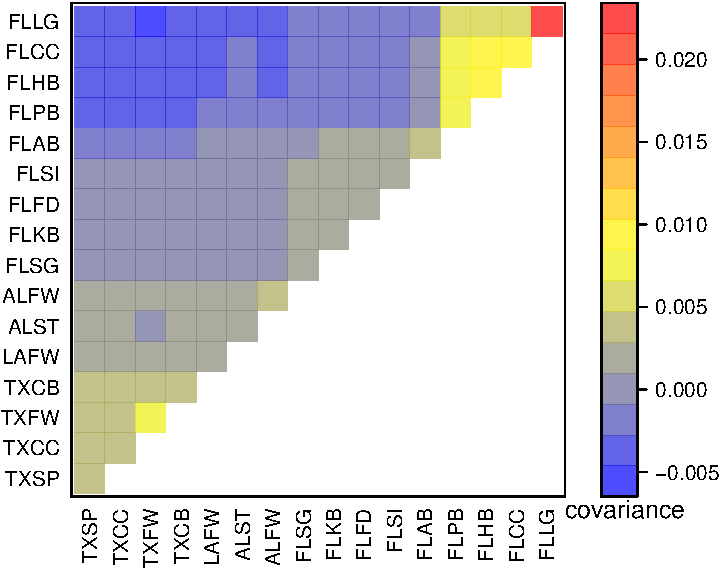
\includegraphics{202_fwsw_reanalysis_files/figure-latex/unnamed-chunk-6-1}

\begin{Shaded}
\begin{Highlighting}[]
\KeywordTok{dimnames}\NormalTok{(nr)[[}\DecValTok{1}\NormalTok{]]<-}\KeywordTok{dimnames}\NormalTok{(nr)[[}\DecValTok{2}\NormalTok{]]<-pop.labs}
\CommentTok{# colors}
\NormalTok{colors<-}\KeywordTok{c}\NormalTok{(}\StringTok{"black"}\NormalTok{,}\StringTok{"darkgrey"}\NormalTok{,}\StringTok{"grey"}\NormalTok{,}\StringTok{"lightgrey"}\NormalTok{,}\StringTok{"cornflowerblue"}\NormalTok{)}
\NormalTok{pal<-}\KeywordTok{colorRampPalette}\NormalTok{(colors)}
\NormalTok{ncol=}\DecValTok{80}
\NormalTok{cols<-}\KeywordTok{pal}\NormalTok{(ncol)}
\NormalTok{rev.colors<-}\KeywordTok{c}\NormalTok{(}\StringTok{"cornflowerblue"}\NormalTok{,}\StringTok{"lightgrey"}\NormalTok{,}\StringTok{"grey"}\NormalTok{,}\StringTok{"darkgrey"}\NormalTok{,}\StringTok{"black"}\NormalTok{)}
\NormalTok{rev.pal<-}\KeywordTok{colorRampPalette}\NormalTok{(rev.colors)}
\NormalTok{rev.cols<-}\KeywordTok{rev.pal}\NormalTok{(ncol)}

\NormalTok{hm.height<-}\KeywordTok{list}\NormalTok{(}\DataTypeTok{x=}\DecValTok{2}\NormalTok{,}\DataTypeTok{units=}\StringTok{"in"}\NormalTok{)}\CommentTok{#2.2/3.8}
\NormalTok{hm.width<-}\KeywordTok{list}\NormalTok{(}\DataTypeTok{x=}\FloatTok{2.4}\NormalTok{,}\DataTypeTok{units=}\StringTok{"in"}\NormalTok{)}\CommentTok{#2.4 in RStudio/3.9}

\NormalTok{heatmaps.name<-}\StringTok{"../figs/fst_heatmaps.png"}

\KeywordTok{png}\NormalTok{(heatmaps.name,}\DataTypeTok{height=}\DecValTok{5}\NormalTok{,}\DataTypeTok{width=}\DecValTok{8}\NormalTok{,}\DataTypeTok{units=}\StringTok{"in"}\NormalTok{,}\DataTypeTok{res=}\DecValTok{300}\NormalTok{)}

\NormalTok{fst.lv<-}\KeywordTok{levelplot}\NormalTok{(}\KeywordTok{as.matrix}\NormalTok{(fst_mat),}\DataTypeTok{col.regions=}\NormalTok{cols,}\DataTypeTok{alpha.regions=}\FloatTok{0.7}\NormalTok{,}
                  \DataTypeTok{scales =} \KeywordTok{list}\NormalTok{(}\DataTypeTok{x=}\KeywordTok{list}\NormalTok{(}\DataTypeTok{rot=}\DecValTok{90}\NormalTok{),}\DataTypeTok{tck =} \DecValTok{0}\NormalTok{),}\DataTypeTok{xlab=}\StringTok{""}\NormalTok{,}\DataTypeTok{ylab=}\StringTok{""}\NormalTok{)}
\KeywordTok{print}\NormalTok{(fst.lv,}\DataTypeTok{split=}\KeywordTok{c}\NormalTok{(}\DecValTok{1}\NormalTok{,}\DecValTok{1}\NormalTok{,}\DecValTok{2}\NormalTok{,}\DecValTok{1}\NormalTok{),}\DataTypeTok{more=}\OtherTok{TRUE}\NormalTok{,}\DataTypeTok{panel.width=}\NormalTok{hm.width,}
      \DataTypeTok{panel.height=}\NormalTok{hm.height,}\DataTypeTok{cex=}\DecValTok{2}\NormalTok{)}
\KeywordTok{trellis.focus}\NormalTok{(}\StringTok{"legend"}\NormalTok{, }\DataTypeTok{side=}\StringTok{"right"}\NormalTok{, }\DataTypeTok{clipp.off=}\OtherTok{TRUE}\NormalTok{, }\DataTypeTok{highlight=}\OtherTok{FALSE}\NormalTok{)}
\KeywordTok{grid.text}\NormalTok{(}\KeywordTok{expression}\NormalTok{(}\KeywordTok{italic}\NormalTok{(F)[ST]), }\FloatTok{0.2}\NormalTok{, }\DecValTok{0}\NormalTok{, }\DataTypeTok{hjust=}\FloatTok{0.5}\NormalTok{, }\DataTypeTok{vjust=}\FloatTok{1.2}\NormalTok{,}\DataTypeTok{gp=}\KeywordTok{gpar}\NormalTok{(}\DataTypeTok{cex=}\FloatTok{0.75}\NormalTok{))}
\KeywordTok{trellis.unfocus}\NormalTok{()}

\NormalTok{nr.lv<-}\KeywordTok{levelplot}\NormalTok{(nr,}\DataTypeTok{col.regions=}\NormalTok{cols,}\DataTypeTok{alpha.regions=}\FloatTok{0.7}\NormalTok{,}
                 \DataTypeTok{scales =} \KeywordTok{list}\NormalTok{(}\DataTypeTok{x=}\KeywordTok{list}\NormalTok{(}\DataTypeTok{rot=}\DecValTok{90}\NormalTok{),}\DataTypeTok{tck =} \DecValTok{0}\NormalTok{),}\DataTypeTok{xlab=}\StringTok{""}\NormalTok{,}\DataTypeTok{ylab=}\StringTok{""}\NormalTok{)}
\KeywordTok{print}\NormalTok{(nr.lv,}\DataTypeTok{split=}\KeywordTok{c}\NormalTok{(}\DecValTok{2}\NormalTok{,}\DecValTok{1}\NormalTok{,}\DecValTok{2}\NormalTok{,}\DecValTok{1}\NormalTok{),}\DataTypeTok{more=}\OtherTok{FALSE}\NormalTok{,}\DataTypeTok{newpage=}\OtherTok{FALSE}\NormalTok{,}\DataTypeTok{panel.width=}\NormalTok{hm.width,}
      \DataTypeTok{panel.height=}\NormalTok{hm.height,}\DataTypeTok{cex=}\DecValTok{2}\NormalTok{)}
\KeywordTok{trellis.focus}\NormalTok{(}\StringTok{"legend"}\NormalTok{, }\DataTypeTok{side=}\StringTok{"right"}\NormalTok{, }\DataTypeTok{clipp.off=}\OtherTok{TRUE}\NormalTok{, }\DataTypeTok{highlight=}\OtherTok{FALSE}\NormalTok{)}
\KeywordTok{grid.text}\NormalTok{(}\StringTok{"Treemix"}\NormalTok{, }\FloatTok{0.2}\NormalTok{, }\DecValTok{0}\NormalTok{, }\DataTypeTok{hjust=}\FloatTok{0.5}\NormalTok{, }\DataTypeTok{vjust=}\FloatTok{1.2}\NormalTok{,}\DataTypeTok{gp=}\KeywordTok{gpar}\NormalTok{(}\DataTypeTok{cex=}\FloatTok{0.75}\NormalTok{))}
\KeywordTok{trellis.unfocus}\NormalTok{()}

\KeywordTok{dev.off}\NormalTok{()}
\end{Highlighting}
\end{Shaded}

\begin{verbatim}
## pdf 
##   2
\end{verbatim}

\href{\%22../figs/fst_heatmaps.png\%22}{!Heatmaps}

\subsubsection{PCAdapt}\label{pcadapt}

\begin{Shaded}
\begin{Highlighting}[]
\KeywordTok{library}\NormalTok{(pcadapt)}
\end{Highlighting}
\end{Shaded}

\begin{Shaded}
\begin{Highlighting}[]
\NormalTok{filename<-}\KeywordTok{read.pcadapt}\NormalTok{(}\StringTok{"filter_rad_20191014@1654/14_filtered/radiator_data_20191014@1710.vcf"}\NormalTok{,}\DataTypeTok{type=}\StringTok{"vcf"}\NormalTok{)}
\end{Highlighting}
\end{Shaded}

\begin{verbatim}
## No variant got discarded.
## Summary:
## 
##  - input file:               filter_rad_20191014@1654/14_filtered/radiator_data_20191014@1710.vcf
##  - output file:              /tmp/RtmpD6D8oD/file540b64657d65.pcadapt
## 
##  - number of individuals detected:   605
##  - number of loci detected:      7433
## 
## 7433 lines detected.
## 605 columns detected.
\end{verbatim}

\begin{Shaded}
\begin{Highlighting}[]
\NormalTok{x<-}\KeywordTok{pcadapt}\NormalTok{(filename, }\DataTypeTok{K=}\DecValTok{20}\NormalTok{)}
\KeywordTok{plot}\NormalTok{(x,}\DataTypeTok{option=}\StringTok{"screeplot"}\NormalTok{) }\CommentTok{#K=7}
\end{Highlighting}
\end{Shaded}

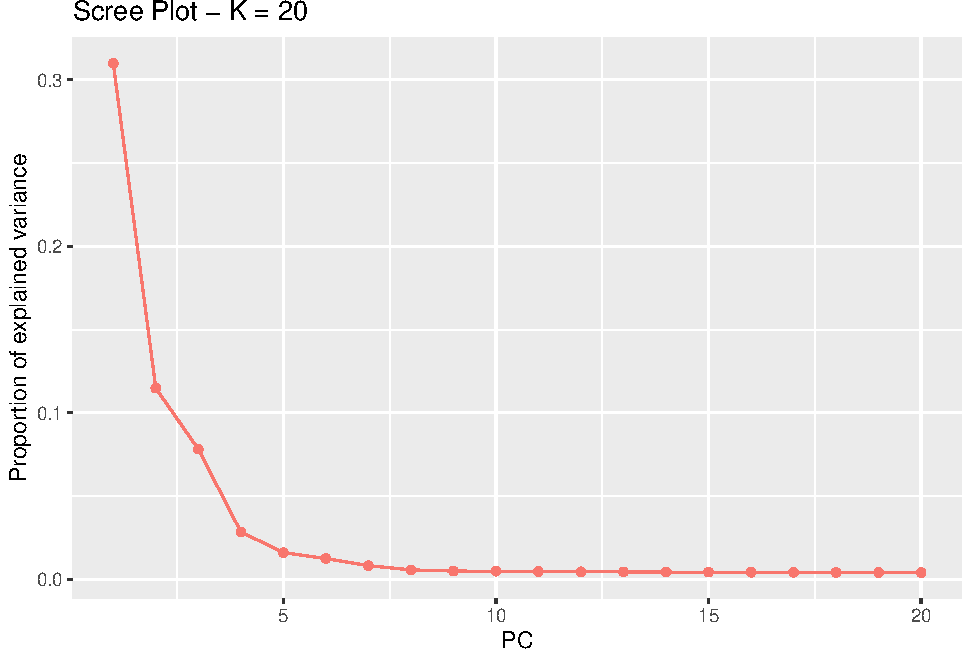
\includegraphics{202_fwsw_reanalysis_files/figure-latex/pcadapt_choose-1}

\begin{Shaded}
\begin{Highlighting}[]
\NormalTok{pa<-}\KeywordTok{pcadapt}\NormalTok{(filename,}\DataTypeTok{K=}\DecValTok{7}\NormalTok{)}
\KeywordTok{saveRDS}\NormalTok{(pa,}\StringTok{"fwsw_all_pcadapt.RDS"}\NormalTok{)}
\NormalTok{pa.props<-}\KeywordTok{round}\NormalTok{((pa}\OperatorTok{$}\NormalTok{singular.values}\OperatorTok{/}\KeywordTok{sum}\NormalTok{(pa}\OperatorTok{$}\NormalTok{singular.values))}\OperatorTok{*}\DecValTok{100}\NormalTok{,}\DecValTok{2}\NormalTok{)}
\NormalTok{pa.props}
\end{Highlighting}
\end{Shaded}

\begin{verbatim}
## [1] 33.26 20.25 16.71 10.09  7.58  6.68  5.43
\end{verbatim}

\begin{Shaded}
\begin{Highlighting}[]
\NormalTok{ind_dat<-}\KeywordTok{read.table}\NormalTok{(}\StringTok{"filter_rad_20191014@1654/14_filtered/individuals.qc.stats_20191014@1654.tsv"}\NormalTok{,}\DataTypeTok{header=}\NormalTok{T,}
                    \DataTypeTok{stringsAsFactors =}\NormalTok{ F)}
\NormalTok{pops<-ind_dat}\OperatorTok{$}\NormalTok{STRATA    }
\NormalTok{grp<-pops}
\NormalTok{grp[grp}\OperatorTok{==}\StringTok{"TXFW"} \OperatorTok{|}\StringTok{ }\NormalTok{grp}\OperatorTok{==}\StringTok{"LAFW"} \OperatorTok{|}\StringTok{ }\NormalTok{grp}\OperatorTok{==}\StringTok{"ALFW"} \OperatorTok{|}\StringTok{ }\NormalTok{grp}\OperatorTok{==}\StringTok{"FLLG"}\NormalTok{]<-}\StringTok{"freshwater"}
\NormalTok{grp[grp}\OperatorTok{!=}\StringTok{"freshwater"}\NormalTok{]<-}\StringTok{"saltwater"}

\CommentTok{#colors}
\NormalTok{pap<-}\KeywordTok{data.frame}\NormalTok{(}\DataTypeTok{Pop=}\NormalTok{pops,}\DataTypeTok{cols=}\NormalTok{pops,}\DataTypeTok{pch=}\NormalTok{pops,}\DataTypeTok{grp=}\NormalTok{grp,}\DataTypeTok{stringsAsFactors =}\NormalTok{ F)}
\NormalTok{pap}\OperatorTok{$}\NormalTok{Pop[pap}\OperatorTok{$}\NormalTok{Pop }\OperatorTok{==}\StringTok{ "FLLG"}\NormalTok{]<-}\StringTok{"FLFW"}
\ControlFlowTok{for}\NormalTok{(i }\ControlFlowTok{in} \DecValTok{1}\OperatorTok{:}\KeywordTok{nrow}\NormalTok{(pap))\{}
\NormalTok{  pap[i,}\StringTok{"cols"}\NormalTok{]<-}\KeywordTok{as.character}\NormalTok{(ppi[ppi}\OperatorTok{$}\NormalTok{Pop }\OperatorTok\StringTok{ }\NormalTok{pap[i,}\StringTok{"Pop"}\NormalTok{],}\StringTok{"cols"}\NormalTok{])}
\NormalTok{\}}
\ControlFlowTok{for}\NormalTok{(i }\ControlFlowTok{in} \DecValTok{1}\OperatorTok{:}\KeywordTok{nrow}\NormalTok{(pap))\{}
\NormalTok{  pap[i,}\StringTok{"pch"}\NormalTok{]<-}\KeywordTok{as.numeric}\NormalTok{(ppi[ppi}\OperatorTok{$}\NormalTok{Pop }\OperatorTok\StringTok{ }\NormalTok{pap[i,}\StringTok{"Pop"}\NormalTok{],}\StringTok{"pch"}\NormalTok{])}
\NormalTok{\}}
\KeywordTok{write.table}\NormalTok{(pap,}\StringTok{"pcadapt_colp.txt"}\NormalTok{,}\DataTypeTok{col.names=}\OtherTok{TRUE}\NormalTok{,}\DataTypeTok{sep=}\StringTok{'}\CharTok{\textbackslash{}t}\StringTok{'}\NormalTok{,}\DataTypeTok{quote=}\NormalTok{F)}
\end{Highlighting}
\end{Shaded}

\begin{Shaded}
\begin{Highlighting}[]
\CommentTok{#plot}
\KeywordTok{par}\NormalTok{(}\DataTypeTok{mfrow=}\KeywordTok{c}\NormalTok{(}\DecValTok{2}\NormalTok{,}\DecValTok{3}\NormalTok{),}\DataTypeTok{oma=}\KeywordTok{c}\NormalTok{(}\DecValTok{2}\NormalTok{,}\DecValTok{2}\NormalTok{,}\DecValTok{2}\NormalTok{,}\DecValTok{2}\NormalTok{),}\DataTypeTok{mar=}\KeywordTok{c}\NormalTok{(}\DecValTok{2}\NormalTok{,}\DecValTok{2}\NormalTok{,}\DecValTok{2}\NormalTok{,}\DecValTok{2}\NormalTok{))}
\KeywordTok{plot}\NormalTok{(pa}\OperatorTok{$}\NormalTok{scores[,}\DecValTok{1}\NormalTok{],pa}\OperatorTok{$}\NormalTok{scores[,}\DecValTok{2}\NormalTok{],}\DataTypeTok{col=}\KeywordTok{alpha}\NormalTok{(pap}\OperatorTok{$}\NormalTok{cols,}\FloatTok{0.5}\NormalTok{),}\DataTypeTok{bg=}\KeywordTok{alpha}\NormalTok{(pap}\OperatorTok{$}\NormalTok{cols,}\FloatTok{0.75}\NormalTok{),}
     \DataTypeTok{pch=}\KeywordTok{as.numeric}\NormalTok{(pap}\OperatorTok{$}\NormalTok{pch),   }\DataTypeTok{cex=}\FloatTok{1.5}\NormalTok{)}
\KeywordTok{mtext}\NormalTok{(}\KeywordTok{paste}\NormalTok{(}\StringTok{"PC1 ("}\NormalTok{,pa.props[}\DecValTok{1}\NormalTok{],}\StringTok{"%)"}\NormalTok{,}\DataTypeTok{sep=}\StringTok{""}\NormalTok{),}\DecValTok{1}\NormalTok{,}\DataTypeTok{line =} \DecValTok{2}\NormalTok{,}\DataTypeTok{cex=}\FloatTok{0.75}\NormalTok{)}
\KeywordTok{mtext}\NormalTok{(}\KeywordTok{paste}\NormalTok{(}\StringTok{"PC2 ("}\NormalTok{,pa.props[}\DecValTok{2}\NormalTok{],}\StringTok{"%)"}\NormalTok{,}\DataTypeTok{sep=}\StringTok{""}\NormalTok{),}\DecValTok{2}\NormalTok{,}\DataTypeTok{line =} \DecValTok{2}\NormalTok{,}\DataTypeTok{cex=}\FloatTok{0.75}\NormalTok{)}
\KeywordTok{plot}\NormalTok{(pa}\OperatorTok{$}\NormalTok{scores[,}\DecValTok{1}\NormalTok{],pa}\OperatorTok{$}\NormalTok{scores[,}\DecValTok{3}\NormalTok{],}\DataTypeTok{col=}\KeywordTok{alpha}\NormalTok{(pap}\OperatorTok{$}\NormalTok{cols,}\FloatTok{0.5}\NormalTok{),}\DataTypeTok{bg=}\KeywordTok{alpha}\NormalTok{(pap}\OperatorTok{$}\NormalTok{cols,}\FloatTok{0.75}\NormalTok{),}\DataTypeTok{pch=}\KeywordTok{as.numeric}\NormalTok{(pap}\OperatorTok{$}\NormalTok{pch),}
    \DataTypeTok{cex=}\FloatTok{1.5}\NormalTok{)}
\KeywordTok{mtext}\NormalTok{(}\KeywordTok{paste}\NormalTok{(}\StringTok{"PC1 ("}\NormalTok{,pa.props[}\DecValTok{1}\NormalTok{],}\StringTok{"%)"}\NormalTok{,}\DataTypeTok{sep=}\StringTok{""}\NormalTok{),}\DecValTok{1}\NormalTok{,}\DataTypeTok{line =} \DecValTok{2}\NormalTok{,}\DataTypeTok{cex=}\FloatTok{0.75}\NormalTok{)}
\KeywordTok{mtext}\NormalTok{(}\KeywordTok{paste}\NormalTok{(}\StringTok{"PC3 ("}\NormalTok{,pa.props[}\DecValTok{3}\NormalTok{],}\StringTok{"%)"}\NormalTok{,}\DataTypeTok{sep=}\StringTok{""}\NormalTok{),}\DecValTok{2}\NormalTok{,}\DataTypeTok{line =} \DecValTok{2}\NormalTok{,}\DataTypeTok{cex=}\FloatTok{0.75}\NormalTok{)}
\KeywordTok{plot}\NormalTok{(pa}\OperatorTok{$}\NormalTok{scores[,}\DecValTok{1}\NormalTok{],pa}\OperatorTok{$}\NormalTok{scores[,}\DecValTok{4}\NormalTok{],}\DataTypeTok{col=}\KeywordTok{alpha}\NormalTok{(pap}\OperatorTok{$}\NormalTok{cols,}\FloatTok{0.5}\NormalTok{),}\DataTypeTok{bg=}\KeywordTok{alpha}\NormalTok{(pap}\OperatorTok{$}\NormalTok{cols,}\FloatTok{0.75}\NormalTok{),}\DataTypeTok{pch=}\KeywordTok{as.numeric}\NormalTok{(pap}\OperatorTok{$}\NormalTok{pch),}
    \DataTypeTok{cex=}\FloatTok{1.5}\NormalTok{)}
\KeywordTok{mtext}\NormalTok{(}\KeywordTok{paste}\NormalTok{(}\StringTok{"PC1 ("}\NormalTok{,pa.props[}\DecValTok{1}\NormalTok{],}\StringTok{"%)"}\NormalTok{,}\DataTypeTok{sep=}\StringTok{""}\NormalTok{),}\DecValTok{1}\NormalTok{,}\DataTypeTok{line =} \DecValTok{2}\NormalTok{,}\DataTypeTok{cex=}\FloatTok{0.75}\NormalTok{)}
\KeywordTok{mtext}\NormalTok{(}\KeywordTok{paste}\NormalTok{(}\StringTok{"PC4 ("}\NormalTok{,pa.props[}\DecValTok{4}\NormalTok{],}\StringTok{"%)"}\NormalTok{,}\DataTypeTok{sep=}\StringTok{""}\NormalTok{),}\DecValTok{2}\NormalTok{,}\DataTypeTok{line =} \DecValTok{2}\NormalTok{,}\DataTypeTok{cex=}\FloatTok{0.75}\NormalTok{)}
\KeywordTok{plot}\NormalTok{(pa}\OperatorTok{$}\NormalTok{scores[grp}\OperatorTok{==}\StringTok{"freshwater"}\NormalTok{,}\DecValTok{1}\NormalTok{],pa}\OperatorTok{$}\NormalTok{scores[grp}\OperatorTok{==}\StringTok{"freshwater"}\NormalTok{,}\DecValTok{2}\NormalTok{],}
     \DataTypeTok{col=}\KeywordTok{alpha}\NormalTok{(pap}\OperatorTok{$}\NormalTok{cols[pap}\OperatorTok{$}\NormalTok{grp}\OperatorTok{==}\StringTok{"freshwater"}\NormalTok{],}\FloatTok{0.5}\NormalTok{),}
     \DataTypeTok{bg=}\KeywordTok{alpha}\NormalTok{(pap}\OperatorTok{$}\NormalTok{cols[pap}\OperatorTok{$}\NormalTok{grp}\OperatorTok{==}\StringTok{"freshwater"}\NormalTok{],}\FloatTok{0.75}\NormalTok{),}\DataTypeTok{pch=}\KeywordTok{as.numeric}\NormalTok{(pap}\OperatorTok{$}\NormalTok{pch[pap}\OperatorTok{$}\NormalTok{grp}\OperatorTok{==}\StringTok{"freshwater"}\NormalTok{]),}
    \DataTypeTok{cex=}\FloatTok{1.5}\NormalTok{)}
\KeywordTok{mtext}\NormalTok{(}\KeywordTok{paste}\NormalTok{(}\StringTok{"PC1 ("}\NormalTok{,pa.props[}\DecValTok{1}\NormalTok{],}\StringTok{"%)"}\NormalTok{,}\DataTypeTok{sep=}\StringTok{""}\NormalTok{),}\DecValTok{1}\NormalTok{,}\DataTypeTok{line =} \DecValTok{2}\NormalTok{,}\DataTypeTok{cex=}\FloatTok{0.75}\NormalTok{)}
\KeywordTok{mtext}\NormalTok{(}\KeywordTok{paste}\NormalTok{(}\StringTok{"PC2 ("}\NormalTok{,pa.props[}\DecValTok{2}\NormalTok{],}\StringTok{"%)"}\NormalTok{,}\DataTypeTok{sep=}\StringTok{""}\NormalTok{),}\DecValTok{2}\NormalTok{,}\DataTypeTok{line =} \DecValTok{2}\NormalTok{,}\DataTypeTok{cex=}\FloatTok{0.75}\NormalTok{)}
\KeywordTok{plot}\NormalTok{(pa}\OperatorTok{$}\NormalTok{scores[grp}\OperatorTok{==}\StringTok{"freshwater"}\NormalTok{,}\DecValTok{3}\NormalTok{],pa}\OperatorTok{$}\NormalTok{scores[grp}\OperatorTok{==}\StringTok{"freshwater"}\NormalTok{,}\DecValTok{4}\NormalTok{],}
     \DataTypeTok{col=}\KeywordTok{alpha}\NormalTok{(pap}\OperatorTok{$}\NormalTok{cols[pap}\OperatorTok{$}\NormalTok{grp}\OperatorTok{==}\StringTok{"freshwater"}\NormalTok{],}\FloatTok{0.5}\NormalTok{),}
     \DataTypeTok{bg=}\KeywordTok{alpha}\NormalTok{(pap}\OperatorTok{$}\NormalTok{cols[pap}\OperatorTok{$}\NormalTok{grp}\OperatorTok{==}\StringTok{"freshwater"}\NormalTok{],}\FloatTok{0.75}\NormalTok{),}\DataTypeTok{pch=}\KeywordTok{as.numeric}\NormalTok{(pap}\OperatorTok{$}\NormalTok{pch[pap}\OperatorTok{$}\NormalTok{grp}\OperatorTok{==}\StringTok{"freshwater"}\NormalTok{]),}
    \DataTypeTok{cex=}\FloatTok{1.5}\NormalTok{)}
\KeywordTok{mtext}\NormalTok{(}\KeywordTok{paste}\NormalTok{(}\StringTok{"PC3 ("}\NormalTok{,pa.props[}\DecValTok{3}\NormalTok{],}\StringTok{"%)"}\NormalTok{,}\DataTypeTok{sep=}\StringTok{""}\NormalTok{),}\DecValTok{1}\NormalTok{,}\DataTypeTok{line =} \DecValTok{2}\NormalTok{,}\DataTypeTok{cex=}\FloatTok{0.75}\NormalTok{)}
\KeywordTok{mtext}\NormalTok{(}\KeywordTok{paste}\NormalTok{(}\StringTok{"PC4 ("}\NormalTok{,pa.props[}\DecValTok{4}\NormalTok{],}\StringTok{"%)"}\NormalTok{,}\DataTypeTok{sep=}\StringTok{""}\NormalTok{),}\DecValTok{2}\NormalTok{,}\DataTypeTok{line =} \DecValTok{2}\NormalTok{,}\DataTypeTok{cex=}\FloatTok{0.75}\NormalTok{)}
\KeywordTok{plot}\NormalTok{(pa}\OperatorTok{$}\NormalTok{scores[grp}\OperatorTok{==}\StringTok{"freshwater"}\NormalTok{,}\DecValTok{5}\NormalTok{],pa}\OperatorTok{$}\NormalTok{scores[grp}\OperatorTok{==}\StringTok{"freshwater"}\NormalTok{,}\DecValTok{6}\NormalTok{],}
     \DataTypeTok{col=}\KeywordTok{alpha}\NormalTok{(pap}\OperatorTok{$}\NormalTok{cols[pap}\OperatorTok{$}\NormalTok{grp}\OperatorTok{==}\StringTok{"freshwater"}\NormalTok{],}\FloatTok{0.5}\NormalTok{),}
     \DataTypeTok{bg=}\KeywordTok{alpha}\NormalTok{(pap}\OperatorTok{$}\NormalTok{cols[pap}\OperatorTok{$}\NormalTok{grp}\OperatorTok{==}\StringTok{"freshwater"}\NormalTok{],}\FloatTok{0.75}\NormalTok{),}\DataTypeTok{pch=}\KeywordTok{as.numeric}\NormalTok{(pap}\OperatorTok{$}\NormalTok{pch[pap}\OperatorTok{$}\NormalTok{grp}\OperatorTok{==}\StringTok{"freshwater"}\NormalTok{]),}
    \DataTypeTok{cex=}\FloatTok{1.5}\NormalTok{)}
\KeywordTok{mtext}\NormalTok{(}\KeywordTok{paste}\NormalTok{(}\StringTok{"PC5 ("}\NormalTok{,pa.props[}\DecValTok{5}\NormalTok{],}\StringTok{"%)"}\NormalTok{,}\DataTypeTok{sep=}\StringTok{""}\NormalTok{),}\DecValTok{1}\NormalTok{,}\DataTypeTok{line =} \DecValTok{2}\NormalTok{,}\DataTypeTok{cex=}\FloatTok{0.75}\NormalTok{)}
\KeywordTok{mtext}\NormalTok{(}\KeywordTok{paste}\NormalTok{(}\StringTok{"PC6 ("}\NormalTok{,pa.props[}\DecValTok{2}\NormalTok{],}\StringTok{"%)"}\NormalTok{,}\DataTypeTok{sep=}\StringTok{""}\NormalTok{),}\DecValTok{2}\NormalTok{,}\DataTypeTok{line =} \DecValTok{2}\NormalTok{,}\DataTypeTok{cex=}\FloatTok{0.75}\NormalTok{)}

\KeywordTok{par}\NormalTok{(}\DataTypeTok{fig =} \KeywordTok{c}\NormalTok{(}\DecValTok{0}\NormalTok{, }\DecValTok{1}\NormalTok{, }\DecValTok{0}\NormalTok{, }\DecValTok{1}\NormalTok{), }\DataTypeTok{oma=}\KeywordTok{c}\NormalTok{(}\DecValTok{2}\NormalTok{,}\DecValTok{1}\NormalTok{,}\DecValTok{0}\NormalTok{,}\DecValTok{1}\NormalTok{), }\DataTypeTok{mar =} \KeywordTok{c}\NormalTok{(}\DecValTok{0}\NormalTok{, }\DecValTok{0}\NormalTok{, }\DecValTok{0}\NormalTok{, }\DecValTok{0}\NormalTok{), }\DataTypeTok{new =} \OtherTok{TRUE}\NormalTok{,}
    \DataTypeTok{cex=}\DecValTok{1}\NormalTok{)}
\KeywordTok{plot}\NormalTok{(}\DecValTok{0}\NormalTok{, }\DecValTok{0}\NormalTok{, }\DataTypeTok{type =} \StringTok{"n"}\NormalTok{, }\DataTypeTok{bty =} \StringTok{"n"}\NormalTok{, }\DataTypeTok{xaxt =} \StringTok{"n"}\NormalTok{, }\DataTypeTok{yaxt =} \StringTok{"n"}\NormalTok{)}

\KeywordTok{legend}\NormalTok{(}\StringTok{"top"}\NormalTok{, }\DataTypeTok{legend=}\NormalTok{ppi}\OperatorTok{$}\NormalTok{Pop, }\DataTypeTok{pch=}\KeywordTok{as.numeric}\NormalTok{(ppi}\OperatorTok{$}\NormalTok{pch), }\DataTypeTok{pt.cex=}\FloatTok{1.5}\NormalTok{,}\DataTypeTok{cex=}\FloatTok{0.85}\NormalTok{,}
       \DataTypeTok{col=}\KeywordTok{alpha}\NormalTok{(ppi}\OperatorTok{$}\NormalTok{cols, }\FloatTok{0.5}\NormalTok{),}\DataTypeTok{pt.bg=}\KeywordTok{alpha}\NormalTok{(ppi}\OperatorTok{$}\NormalTok{cols,}\FloatTok{0.25}\NormalTok{), }\DataTypeTok{ncol=}\DecValTok{8}\NormalTok{,}\DataTypeTok{bty=}\StringTok{'n'}\NormalTok{)}
\end{Highlighting}
\end{Shaded}

\includegraphics{../figs/pcadapt.pc1-6plot_pcadapt_initial-1}

\subsubsection{Admixture}\label{admixture}

\begin{Shaded}
\begin{Highlighting}[]
\NormalTok{admixK<-}\KeywordTok{read.delim}\NormalTok{(}\StringTok{"admixture/K_CVs.txt"}\NormalTok{,}\DataTypeTok{header =} \OtherTok{FALSE}\NormalTok{)}
\NormalTok{admixK}\OperatorTok{$}\NormalTok{K<-}\KeywordTok{as.numeric}\NormalTok{(}\KeywordTok{gsub}\NormalTok{(}\StringTok{".*}\CharTok{\textbackslash{}\textbackslash{}}\StringTok{(K=(}\CharTok{\textbackslash{}\textbackslash{}}\StringTok{d+)}\CharTok{\textbackslash{}\textbackslash{}}\StringTok{).*"}\NormalTok{,}\StringTok{"}\CharTok{\textbackslash{}\textbackslash{}}\StringTok{1"}\NormalTok{,admixK}\OperatorTok{$}\NormalTok{V1))}
\NormalTok{admixK}\OperatorTok{$}\NormalTok{CV<-}\KeywordTok{as.numeric}\NormalTok{(}\KeywordTok{gsub}\NormalTok{(}\StringTok{"^.*}\CharTok{\textbackslash{}\textbackslash{}}\StringTok{: (}\CharTok{\textbackslash{}\textbackslash{}}\StringTok{d+}\CharTok{\textbackslash{}\textbackslash{}}\StringTok{.}\CharTok{\textbackslash{}\textbackslash{}}\StringTok{d+)$"}\NormalTok{,}\StringTok{"}\CharTok{\textbackslash{}\textbackslash{}}\StringTok{1"}\NormalTok{,admixK}\OperatorTok{$}\NormalTok{V1))}

\NormalTok{admixK<-admixK[}\KeywordTok{order}\NormalTok{(admixK}\OperatorTok{$}\NormalTok{K),]}

\KeywordTok{plot}\NormalTok{(admixK}\OperatorTok{$}\NormalTok{K,admixK}\OperatorTok{$}\NormalTok{CV,}\DataTypeTok{pch=}\DecValTok{19}\NormalTok{,}\DataTypeTok{type =} \StringTok{"b"}\NormalTok{,}\DataTypeTok{lty=}\DecValTok{1}\NormalTok{,}\DataTypeTok{xlab =} \StringTok{"K"}\NormalTok{,}\DataTypeTok{ylab=}\StringTok{"CV"}\NormalTok{,}\DataTypeTok{las=}\DecValTok{1}\NormalTok{,}\DataTypeTok{lwd=}\DecValTok{2}\NormalTok{)}
\end{Highlighting}
\end{Shaded}

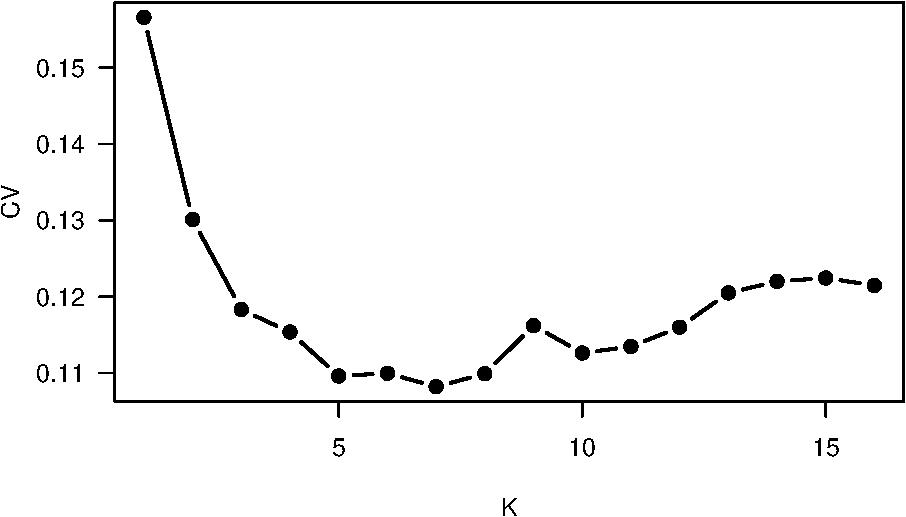
\includegraphics{202_fwsw_reanalysis_files/figure-latex/unnamed-chunk-8-1}

Looks like K=5 or K=7 are the best, let's look at those outputs.

\begin{Shaded}
\begin{Highlighting}[]
\KeywordTok{library}\NormalTok{(RColorBrewer)}
\NormalTok{qfile<-}\StringTok{"admixture/fwsw_all_filt.5.Q"}
\NormalTok{famfile<-}\StringTok{"admixture/fwsw_all_filt.fam"}
\NormalTok{poporderFile<-}\StringTok{"treemix/poplist"}
\NormalTok{K<-}\DecValTok{5}

\CommentTok{# read files in }
\NormalTok{qtbl<-}\KeywordTok{read.table}\NormalTok{(qfile,}\DataTypeTok{stringsAsFactors =}\NormalTok{ F)}
\NormalTok{famTable<-}\StringTok{ }\KeywordTok{read.table}\NormalTok{(famfile,}
                      \DataTypeTok{col.names =} \KeywordTok{c}\NormalTok{(}\StringTok{"Pop"}\NormalTok{,}\StringTok{"Ind"}\NormalTok{,}\StringTok{"Father"}\NormalTok{,}\StringTok{"Mother"}\NormalTok{,}\StringTok{"Sex"}\NormalTok{,}\StringTok{"phenotype"}\NormalTok{),}\DataTypeTok{stringsAsFactors =}\NormalTok{ F)[}\DecValTok{1}\OperatorTok{:}\DecValTok{2}\NormalTok{]}
\NormalTok{poporder<-}\KeywordTok{read.table}\NormalTok{(poporderFile,}\DataTypeTok{col.names =} \KeywordTok{c}\NormalTok{(}\StringTok{"Pop"}\NormalTok{),}\DataTypeTok{stringsAsFactors =}\NormalTok{ F)}
\NormalTok{poporder}\OperatorTok{$}\NormalTok{orderNum<-}\DecValTok{1}\OperatorTok{:}\KeywordTok{nrow}\NormalTok{(poporder)}


\CommentTok{# create useful tables}
\NormalTok{mergedAdmixtureTable <-}\StringTok{ }\KeywordTok{cbind}\NormalTok{(qtbl, famTable)}
\NormalTok{mergedAdmixTabOrderNs <-}\StringTok{ }\KeywordTok{merge}\NormalTok{(mergedAdmixtureTable,poporder,}\DataTypeTok{by=}\StringTok{"Pop"}\NormalTok{)}
\NormalTok{ordered <-}\StringTok{ }\NormalTok{mergedAdmixTabOrderNs[}\KeywordTok{order}\NormalTok{(mergedAdmixTabOrderNs}\OperatorTok{$}\NormalTok{orderNum),]}


\KeywordTok{plotting.structure}\NormalTok{(ordered[,}\DecValTok{1}\OperatorTok{:}\NormalTok{(}\KeywordTok{ncol}\NormalTok{(ordered)}\OperatorTok{-}\DecValTok{2}\NormalTok{)],}\DataTypeTok{k =} \DecValTok{5}\NormalTok{,}\DataTypeTok{pop.order =}\NormalTok{ poporder}\OperatorTok{$}\NormalTok{Pop,}\DataTypeTok{make.file =} \OtherTok{FALSE}\NormalTok{)}
\end{Highlighting}
\end{Shaded}

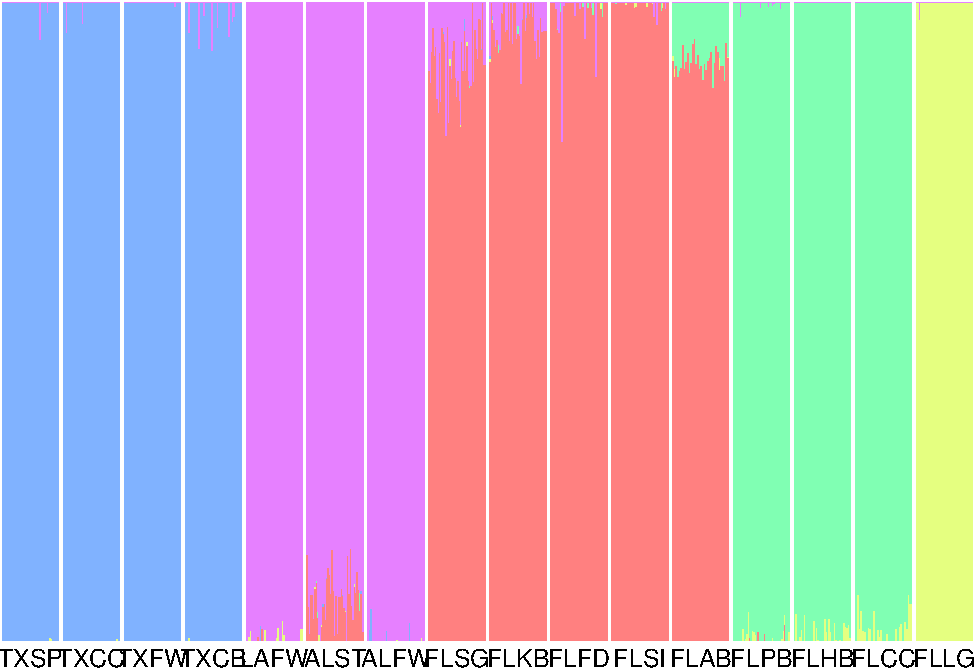
\includegraphics{202_fwsw_reanalysis_files/figure-latex/unnamed-chunk-9-1}

\begin{Shaded}
\begin{Highlighting}[]
\NormalTok{admixK5<-ordered[,}\DecValTok{1}\OperatorTok{:}\NormalTok{(}\KeywordTok{ncol}\NormalTok{(ordered)}\OperatorTok{-}\DecValTok{2}\NormalTok{)]}
\KeywordTok{write.table}\NormalTok{(admixK5,}\StringTok{"admixture/admixK5.txt"}\NormalTok{,}\DataTypeTok{sep =} \StringTok{'}\CharTok{\textbackslash{}t}\StringTok{'}\NormalTok{,}\DataTypeTok{quote =} \OtherTok{FALSE}\NormalTok{,}\DataTypeTok{col.names =} \OtherTok{TRUE}\NormalTok{,}\DataTypeTok{row.names =} \OtherTok{FALSE}\NormalTok{)}
\end{Highlighting}
\end{Shaded}

\begin{Shaded}
\begin{Highlighting}[]
\NormalTok{qfile<-}\StringTok{"admixture/fwsw_all_filt.7.Q"}
\NormalTok{famfile<-}\StringTok{"admixture/fwsw_all_filt.fam"}
\NormalTok{poporderFile<-}\StringTok{"treemix/poplist"}
\NormalTok{K<-}\DecValTok{7}

\CommentTok{# read files in }
\NormalTok{qtbl<-}\KeywordTok{read.table}\NormalTok{(qfile,}\DataTypeTok{stringsAsFactors =}\NormalTok{ F)}
\NormalTok{famTable<-}\StringTok{ }\KeywordTok{read.table}\NormalTok{(famfile,}
                      \DataTypeTok{col.names =} \KeywordTok{c}\NormalTok{(}\StringTok{"Pop"}\NormalTok{,}\StringTok{"Ind"}\NormalTok{,}\StringTok{"Father"}\NormalTok{,}\StringTok{"Mother"}\NormalTok{,}\StringTok{"Sex"}\NormalTok{,}\StringTok{"phenotype"}\NormalTok{),}\DataTypeTok{stringsAsFactors =}\NormalTok{ F)[}\DecValTok{1}\OperatorTok{:}\DecValTok{2}\NormalTok{]}
\NormalTok{poporder<-}\KeywordTok{read.table}\NormalTok{(poporderFile,}\DataTypeTok{col.names =} \KeywordTok{c}\NormalTok{(}\StringTok{"Pop"}\NormalTok{),}\DataTypeTok{stringsAsFactors =}\NormalTok{ F)}
\NormalTok{poporder}\OperatorTok{$}\NormalTok{orderNum<-}\DecValTok{1}\OperatorTok{:}\KeywordTok{nrow}\NormalTok{(poporder)}


\CommentTok{# create useful tables}
\NormalTok{mergedAdmixtureTable <-}\StringTok{ }\KeywordTok{cbind}\NormalTok{(qtbl, famTable)}
\NormalTok{mergedAdmixTabOrderNs <-}\StringTok{ }\KeywordTok{merge}\NormalTok{(mergedAdmixtureTable,poporder,}\DataTypeTok{by=}\StringTok{"Pop"}\NormalTok{)}
\NormalTok{ordered <-}\StringTok{ }\NormalTok{mergedAdmixTabOrderNs[}\KeywordTok{order}\NormalTok{(mergedAdmixTabOrderNs}\OperatorTok{$}\NormalTok{orderNum),]}

\KeywordTok{par}\NormalTok{(}\DataTypeTok{mar=}\KeywordTok{c}\NormalTok{(}\DecValTok{1}\NormalTok{,}\DecValTok{0}\NormalTok{,}\DecValTok{0}\NormalTok{,}\DecValTok{0}\NormalTok{))}
\KeywordTok{plotting.structure}\NormalTok{(ordered[,}\DecValTok{1}\OperatorTok{:}\NormalTok{(}\KeywordTok{ncol}\NormalTok{(ordered)}\OperatorTok{-}\DecValTok{2}\NormalTok{)],}\DataTypeTok{k =} \DecValTok{7}\NormalTok{,}\DataTypeTok{pop.order =}\NormalTok{ poporder}\OperatorTok{$}\NormalTok{Pop,}\DataTypeTok{make.file =} \OtherTok{FALSE}\NormalTok{)}
\NormalTok{admixK7<-ordered[,}\DecValTok{1}\OperatorTok{:}\NormalTok{(}\KeywordTok{ncol}\NormalTok{(ordered)}\OperatorTok{-}\DecValTok{2}\NormalTok{)]}
\KeywordTok{plotting.structure}\NormalTok{(admixK7,}\DataTypeTok{k =} \DecValTok{7}\NormalTok{,}\DataTypeTok{pop.order =}\NormalTok{ poporder}\OperatorTok{$}\NormalTok{Pop,}\DataTypeTok{make.file =} \OtherTok{FALSE}\NormalTok{)}
\end{Highlighting}
\end{Shaded}

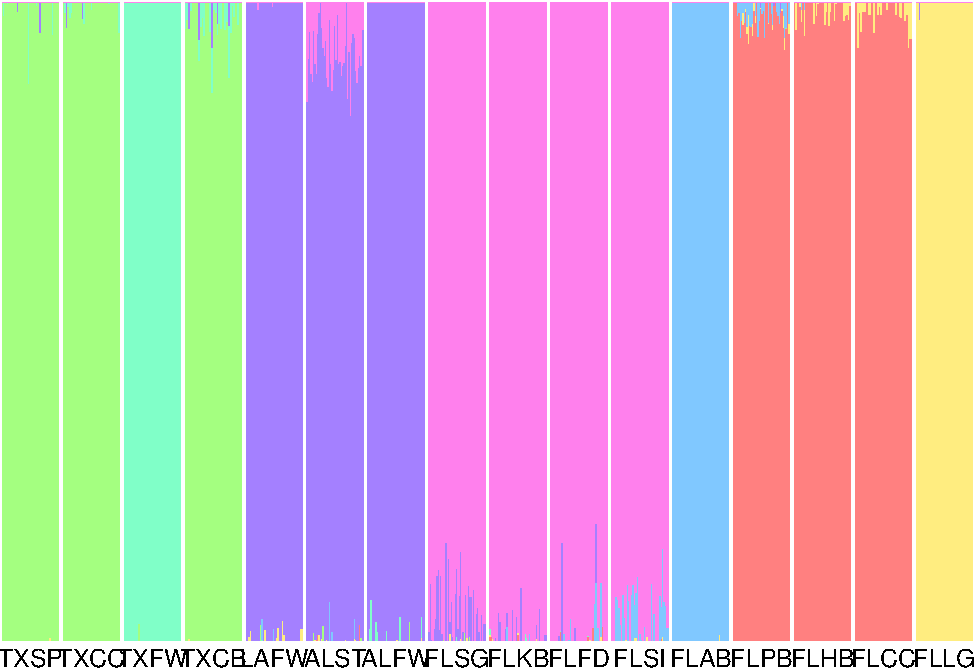
\includegraphics{202_fwsw_reanalysis_files/figure-latex/unnamed-chunk-10-1}

\begin{Shaded}
\begin{Highlighting}[]
\KeywordTok{write.table}\NormalTok{(admixK7,}\StringTok{"admixture/admixK7.txt"}\NormalTok{,}\DataTypeTok{sep =} \StringTok{'}\CharTok{\textbackslash{}t}\StringTok{'}\NormalTok{,}\DataTypeTok{quote =} \OtherTok{FALSE}\NormalTok{,}\DataTypeTok{col.names =} \OtherTok{TRUE}\NormalTok{,}\DataTypeTok{row.names =} \OtherTok{FALSE}\NormalTok{)}
\end{Highlighting}
\end{Shaded}

\subsubsection{Treemix}\label{treemix}

\begin{Shaded}
\begin{Highlighting}[]
\NormalTok{poporder<-}\KeywordTok{c}\NormalTok{(}\StringTok{"TXSP"}\NormalTok{,}\StringTok{"TXCC"}\NormalTok{,}\StringTok{"TXFW"}\NormalTok{,}\StringTok{"TXCB"}\NormalTok{,}\StringTok{"LAFW"}\NormalTok{,}\StringTok{"ALST"}\NormalTok{,}
            \StringTok{"ALFW"}\NormalTok{,}\StringTok{"FLSG"}\NormalTok{,}\StringTok{"FLKB"}\NormalTok{,}\StringTok{"FLFD"}\NormalTok{,}\StringTok{"FLSI"}\NormalTok{,}\StringTok{"FLAB"}\NormalTok{,}
            \StringTok{"FLPB"}\NormalTok{,}\StringTok{"FLHB"}\NormalTok{,}\StringTok{"FLCC"}\NormalTok{,}\StringTok{"FLLG"}\NormalTok{)}
\NormalTok{colors<-poporder}
\NormalTok{colors[colors }\OperatorTok\StringTok{ "FLLG"}\NormalTok{]<-grp.colors[}\DecValTok{6}\NormalTok{]}
\NormalTok{colors[colors }\OperatorTok\StringTok{ }\KeywordTok{c}\NormalTok{(}\StringTok{"FLPB"}\NormalTok{,}\StringTok{"FLHB"}\NormalTok{,}\StringTok{"FLCC"}\NormalTok{)]<-grp.colors[}\DecValTok{6}\NormalTok{]}
\NormalTok{colors[colors }\OperatorTok\StringTok{ }\KeywordTok{c}\NormalTok{(}\StringTok{"FLAB"}\NormalTok{)]<-grp.colors[}\DecValTok{5}\NormalTok{]}
\NormalTok{colors[colors }\OperatorTok\StringTok{ }\KeywordTok{c}\NormalTok{(}\StringTok{"FLSI"}\NormalTok{,}\StringTok{"FLFD"}\NormalTok{,}\StringTok{"FLKB"}\NormalTok{,}\StringTok{"FLSG"}\NormalTok{)]<-grp.colors[}\DecValTok{3}\NormalTok{]}
\NormalTok{colors[colors }\OperatorTok\StringTok{ }\KeywordTok{c}\NormalTok{(}\StringTok{"ALST"}\NormalTok{,}\StringTok{"ALFW"}\NormalTok{,}\StringTok{"LAFW"}\NormalTok{)]<-grp.colors[}\DecValTok{2}\NormalTok{]}
\NormalTok{colors[colors }\OperatorTok\StringTok{ }\KeywordTok{c}\NormalTok{(}\StringTok{"TXSP"}\NormalTok{,}\StringTok{"TXCC"}\NormalTok{,}\StringTok{"TXFW"}\NormalTok{,}\StringTok{"TXCB"}\NormalTok{)]<-grp.colors[}\DecValTok{1}\NormalTok{]}
\KeywordTok{write.table}\NormalTok{(}\KeywordTok{cbind}\NormalTok{(poporder,colors),}\StringTok{"poporder"}\NormalTok{,}\DataTypeTok{quote=}\NormalTok{F,}\DataTypeTok{sep=}\StringTok{'}\CharTok{\textbackslash{}t}\StringTok{'}\NormalTok{)}
\end{Highlighting}
\end{Shaded}

\begin{Shaded}
\begin{Highlighting}[]
\KeywordTok{source}\NormalTok{(}\StringTok{"../R/203_treemix_plotting_funcs.R"}\NormalTok{) }\CommentTok{#I've modified the functions from treemix}
\KeywordTok{library}\NormalTok{(lattice); }\KeywordTok{library}\NormalTok{(grid); }\KeywordTok{library}\NormalTok{(RColorBrewer)}
\NormalTok{poporder<-}\KeywordTok{read.delim}\NormalTok{(}\StringTok{"treemix/poporder"}\NormalTok{)}
\NormalTok{colors<-poporder}\OperatorTok{$}\NormalTok{colors}
\NormalTok{poporder<-poporder}\OperatorTok{$}\NormalTok{poporder}
\KeywordTok{par}\NormalTok{(}\DataTypeTok{mfrow=}\KeywordTok{c}\NormalTok{(}\DecValTok{1}\NormalTok{,}\DecValTok{2}\NormalTok{),}\DataTypeTok{oma=}\KeywordTok{c}\NormalTok{(}\DecValTok{2}\NormalTok{,}\DecValTok{2}\NormalTok{,}\DecValTok{2}\NormalTok{,}\DecValTok{2}\NormalTok{),}\DataTypeTok{mar=}\KeywordTok{c}\NormalTok{(}\DecValTok{2}\NormalTok{,}\DecValTok{2}\NormalTok{,}\DecValTok{2}\NormalTok{,}\DecValTok{2}\NormalTok{))}
\NormalTok{tree<-}\KeywordTok{plot_tree}\NormalTok{(}\StringTok{"treemix/fwsw_k100b"}\NormalTok{,}\DataTypeTok{plotmig=}\NormalTok{F,}\DataTypeTok{scale=}\NormalTok{F,}\DataTypeTok{mbar=}\NormalTok{F,}\DataTypeTok{plus=}\FloatTok{0.05}\NormalTok{)}
\end{Highlighting}
\end{Shaded}

\begin{verbatim}
##     V1   V2       V3      V4      V5  V6  V7 V8  V9 V10
## 1    0 <NA>     ROOT NOT_MIG NOT_TIP   0 304  3 472  13
## 2    1 FLHB NOT_ROOT NOT_MIG     TIP 172  NA NA  NA  NA
## 3    2 <NA> NOT_ROOT NOT_MIG NOT_TIP 356 104  7 256   2
## 4    3 LAFW NOT_ROOT NOT_MIG     TIP 412  NA NA  NA  NA
## 5    4 TXSP NOT_ROOT NOT_MIG     TIP  52  NA NA  NA  NA
## 6   15 FLAB NOT_ROOT NOT_MIG     TIP  76  NA NA  NA  NA
## 7   16 <NA> NOT_ROOT NOT_MIG NOT_TIP 472 356 10 412   2
## 8   31 FLLG NOT_ROOT NOT_MIG     TIP  32  NA NA  NA  NA
## 9   32 <NA> NOT_ROOT NOT_MIG NOT_TIP  76  31  1 136   3
## 10  51 TXCC NOT_ROOT NOT_MIG     TIP  52  NA NA  NA  NA
## 11  52 <NA> NOT_ROOT NOT_MIG NOT_TIP 304   4  1  51   1
## 12  75 FLFD NOT_ROOT NOT_MIG     TIP 212  NA NA  NA  NA
## 13  76 <NA> NOT_ROOT NOT_MIG NOT_TIP 104  15  1  32   4
## 14 103 FLKB NOT_ROOT NOT_MIG     TIP 256  NA NA  NA  NA
## 15 104 <NA> NOT_ROOT NOT_MIG NOT_TIP   2  76  5 212   2
## 16 135 FLPB NOT_ROOT NOT_MIG     TIP 136  NA NA  NA  NA
## 17 136 <NA> NOT_ROOT NOT_MIG NOT_TIP  32 135  1 172   2
## 18 171 FLCC NOT_ROOT NOT_MIG     TIP 172  NA NA  NA  NA
## 19 172 <NA> NOT_ROOT NOT_MIG NOT_TIP 136   1  1 171   1
## 20 211 FLSI NOT_ROOT NOT_MIG     TIP 212  NA NA  NA  NA
## 21 212 <NA> NOT_ROOT NOT_MIG NOT_TIP 104  75  1 211   1
## 22 255 FLSG NOT_ROOT NOT_MIG     TIP 256  NA NA  NA  NA
## 23 256 <NA> NOT_ROOT NOT_MIG NOT_TIP   2 103  1 255   1
## 24 303 TXCB NOT_ROOT NOT_MIG     TIP 304  NA NA  NA  NA
## 25 304 <NA> NOT_ROOT NOT_MIG NOT_TIP   0  52  2 303   1
## 26 355 ALST NOT_ROOT NOT_MIG     TIP 356  NA NA  NA  NA
## 27 356 <NA> NOT_ROOT NOT_MIG NOT_TIP  16   2  9 355   1
## 28 411 ALFW NOT_ROOT NOT_MIG     TIP 412  NA NA  NA  NA
## 29 412 <NA> NOT_ROOT NOT_MIG NOT_TIP  16   3  1 411   1
## 30 471 TXFW NOT_ROOT NOT_MIG     TIP 472  NA NA  NA  NA
## 31 472 <NA> NOT_ROOT NOT_MIG NOT_TIP   0  16 12 471   1
##                                                                                                                                                                                                                                                                                                                                                                                                                                           V11
## 1  (((TXSP:0.000131454,TXCC:0):0.000527644,TXCB:0.00044987):0.000275279,((((((FLAB:0.001625,(FLLG:0.0165286,(FLPB:0,(FLHB:4.0731e-05,FLCC:8.16396e-05):0.000949241):0.00146329):0.00951218):0.00153256,(FLFD:0,FLSI:0.000288953):0.000811088):0.000242145,(FLKB:0.000166115,FLSG:7.91444e-05):0.000500389):0.0026018,ALST:6.80349e-05):0.000535248,(LAFW:0.000401198,ALFW:0.000609201):0.000353502):0.00263375,TXFW:0.00468318):0.000275279);
## 2                                                                                                                                                                                                                                                                                                                                                                                                                             FLHB:4.0731e-05
## 3                                                                                                                                                                                                   (((FLAB:0.001625,(FLLG:0.0165286,(FLPB:0,(FLHB:4.0731e-05,FLCC:8.16396e-05):0.000949241):0.00146329):0.00951218):0.00153256,(FLFD:0,FLSI:0.000288953):0.000811088):0.000242145,(FLKB:0.000166115,FLSG:7.91444e-05):0.000500389):0.0026018
## 4                                                                                                                                                                                                                                                                                                                                                                                                                            LAFW:0.000401198
## 5                                                                                                                                                                                                                                                                                                                                                                                                                            TXSP:0.000131454
## 6                                                                                                                                                                                                                                                                                                                                                                                                                               FLAB:0.001625
## 7                                                                                                       (((((FLAB:0.001625,(FLLG:0.0165286,(FLPB:0,(FLHB:4.0731e-05,FLCC:8.16396e-05):0.000949241):0.00146329):0.00951218):0.00153256,(FLFD:0,FLSI:0.000288953):0.000811088):0.000242145,(FLKB:0.000166115,FLSG:7.91444e-05):0.000500389):0.0026018,ALST:6.80349e-05):0.000535248,(LAFW:0.000401198,ALFW:0.000609201):0.000353502):0.00263375
## 8                                                                                                                                                                                                                                                                                                                                                                                                                              FLLG:0.0165286
## 9                                                                                                                                                                                                                                                                                                                                              (FLLG:0.0165286,(FLPB:0,(FLHB:4.0731e-05,FLCC:8.16396e-05):0.000949241):0.00146329):0.00951218
## 10                                                                                                                                                                                                                                                                                                                                                                                                                                     TXCC:0
## 11                                                                                                                                                                                                                                                                                                                                                                                                      (TXSP:0.000131454,TXCC:0):0.000527644
## 12                                                                                                                                                                                                                                                                                                                                                                                                                                     FLFD:0
## 13                                                                                                                                                                                                                                                                                                                  (FLAB:0.001625,(FLLG:0.0165286,(FLPB:0,(FLHB:4.0731e-05,FLCC:8.16396e-05):0.000949241):0.00146329):0.00951218):0.00153256
## 14                                                                                                                                                                                                                                                                                                                                                                                                                           FLKB:0.000166115
## 15                                                                                                                                                                                                                                                              ((FLAB:0.001625,(FLLG:0.0165286,(FLPB:0,(FLHB:4.0731e-05,FLCC:8.16396e-05):0.000949241):0.00146329):0.00951218):0.00153256,(FLFD:0,FLSI:0.000288953):0.000811088):0.000242145
## 16                                                                                                                                                                                                                                                                                                                                                                                                                                     FLPB:0
## 17                                                                                                                                                                                                                                                                                                                                                                         (FLPB:0,(FLHB:4.0731e-05,FLCC:8.16396e-05):0.000949241):0.00146329
## 18                                                                                                                                                                                                                                                                                                                                                                                                                           FLCC:8.16396e-05
## 19                                                                                                                                                                                                                                                                                                                                                                                             (FLHB:4.0731e-05,FLCC:8.16396e-05):0.000949241
## 20                                                                                                                                                                                                                                                                                                                                                                                                                           FLSI:0.000288953
## 21                                                                                                                                                                                                                                                                                                                                                                                                      (FLFD:0,FLSI:0.000288953):0.000811088
## 22                                                                                                                                                                                                                                                                                                                                                                                                                           FLSG:7.91444e-05
## 23                                                                                                                                                                                                                                                                                                                                                                                            (FLKB:0.000166115,FLSG:7.91444e-05):0.000500389
## 24                                                                                                                                                                                                                                                                                                                                                                                                                            TXCB:0.00044987
## 25                                                                                                                                                                                                                                                                                                                                                                        ((TXSP:0.000131454,TXCC:0):0.000527644,TXCB:0.00044987):0.000275279
## 26                                                                                                                                                                                                                                                                                                                                                                                                                           ALST:6.80349e-05
## 27                                                                                                                                                                   ((((FLAB:0.001625,(FLLG:0.0165286,(FLPB:0,(FLHB:4.0731e-05,FLCC:8.16396e-05):0.000949241):0.00146329):0.00951218):0.00153256,(FLFD:0,FLSI:0.000288953):0.000811088):0.000242145,(FLKB:0.000166115,FLSG:7.91444e-05):0.000500389):0.0026018,ALST:6.80349e-05):0.000535248
## 28                                                                                                                                                                                                                                                                                                                                                                                                                           ALFW:0.000609201
## 29                                                                                                                                                                                                                                                                                                                                                                                            (LAFW:0.000401198,ALFW:0.000609201):0.000353502
## 30                                                                                                                                                                                                                                                                                                                                                                                                                            TXFW:0.00468318
## 31                                                                        ((((((FLAB:0.001625,(FLLG:0.0165286,(FLPB:0,(FLHB:4.0731e-05,FLCC:8.16396e-05):0.000949241):0.00146329):0.00951218):0.00153256,(FLFD:0,FLSI:0.000288953):0.000811088):0.000242145,(FLKB:0.000166115,FLSG:7.91444e-05):0.000500389):0.0026018,ALST:6.80349e-05):0.000535248,(LAFW:0.000401198,ALFW:0.000609201):0.000353502):0.00263375,TXFW:0.00468318):0.000275279
##              x       y   ymin   ymax
## 1  0.000000000 0.81250 0.0000 1.0000
## 2  0.019786224 0.59375 0.5625 0.6250
## 3  0.006046077 0.37500 0.2500 0.8125
## 4  0.003663729 0.15625 0.1250 0.1875
## 5  0.000934377 0.96875 0.9375 1.0000
## 6  0.009445782 0.78125 0.7500 0.8125
## 7  0.002909029 0.18750 0.0625 0.8125
## 8  0.033861562 0.71875 0.6875 0.7500
## 9  0.017332962 0.68750 0.5000 0.7500
## 10 0.000802923 0.90625 0.8750 0.9375
## 11 0.000802923 0.93750 0.8750 1.0000
## 12 0.007099310 0.46875 0.4375 0.5000
## 13 0.007820782 0.75000 0.5000 0.8125
## 14 0.006712581 0.34375 0.3125 0.3750
## 15 0.006288222 0.50000 0.3750 0.8125
## 16 0.018796252 0.65625 0.6250 0.6875
## 17 0.018796252 0.62500 0.5000 0.6875
## 18 0.019827133 0.53125 0.5000 0.5625
## 19 0.019745493 0.56250 0.5000 0.6250
## 20 0.007388263 0.40625 0.3750 0.4375
## 21 0.007099310 0.43750 0.3750 0.5000
## 22 0.006625610 0.28125 0.2500 0.3125
## 23 0.006546466 0.31250 0.2500 0.3750
## 24 0.000725149 0.84375 0.8125 0.8750
## 25 0.000275279 0.87500 0.8125 1.0000
## 26 0.003512312 0.21875 0.1875 0.2500
## 27 0.003444277 0.25000 0.1875 0.8125
## 28 0.003871732 0.09375 0.0625 0.1250
## 29 0.003262531 0.12500 0.0625 0.1875
## 30 0.004958459 0.03125 0.0000 0.0625
## 31 0.000275279 0.06250 0.0000 0.8125
\end{verbatim}

\begin{verbatim}
##  [1] 0.019786224 0.003663729 0.000934377 0.009445782 0.033861562
##  [6] 0.000802923 0.007099310 0.006712581 0.018796252 0.019827133
## [11] 0.007388263 0.006625610 0.000725149 0.003512312 0.003871732
## [16] 0.004958459
## [1] 0.003
\end{verbatim}

\begin{Shaded}
\begin{Highlighting}[]
\KeywordTok{mtext}\NormalTok{(}\StringTok{"Drift parameter"}\NormalTok{,}\DecValTok{1}\NormalTok{,}\DataTypeTok{line=}\DecValTok{2}\NormalTok{)}
\NormalTok{resid<-}\KeywordTok{plot_resid}\NormalTok{(}\StringTok{"treemix/fwsw_k100b"}\NormalTok{,}\StringTok{"treemix/poporder"}\NormalTok{,}\DataTypeTok{wcols=}\StringTok{"rb"}\NormalTok{)}
\end{Highlighting}
\end{Shaded}

\begin{verbatim}
## [1] 0.0001958949
## [1] "here"
\end{verbatim}

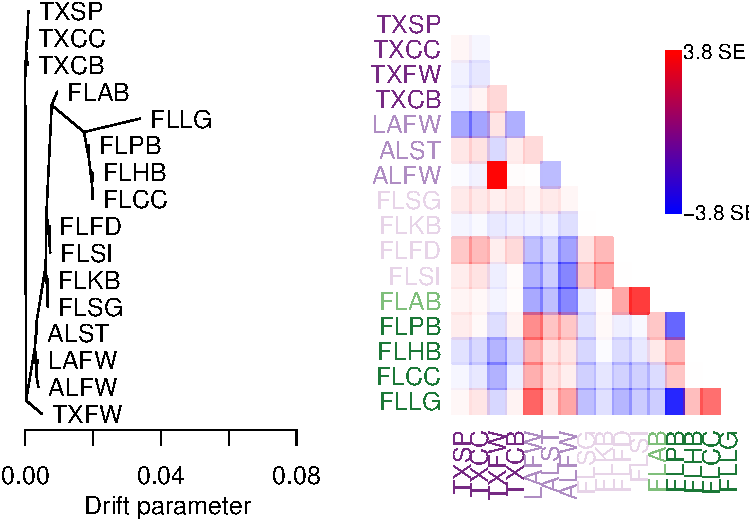
\includegraphics{202_fwsw_reanalysis_files/figure-latex/treemixPrep-1}

\begin{verbatim}
## [1] "1 1 9.40000000000489e-07"
## [1] "2 1 2.45699999999998e-05"
## [1] "2 2 -2.497e-05"
## [1] "3 1 -3.98099999999999e-05"
## [1] "3 2 -6.78499999999999e-05"
## [1] "3 3 9.39999999999622e-07"
## [1] "4 1 -2.86500000000003e-05"
## [1] "4 2 3.081e-05"
## [1] "4 3 0.00011171"
## [1] "4 4 9.40000000000489e-07"
## [1] "5 1 -0.00025325"
## [1] "5 2 -0.000264"
## [1] "5 3 7.909e-05"
## [1] "5 4 -0.00023061"
## [1] "5 5 9.49999999999996e-07"
## [1] "6 1 7.006e-05"
## [1] "6 2 8.413e-05"
## [1] "6 3 -0.000109987"
## [1] "6 4 5.22300000000001e-05"
## [1] "6 5 0.00010773"
## [1] "6 6 9.49999999999996e-07"
## [1] "7 1 -1.17499999999998e-05"
## [1] "7 2 -3.73600000000002e-05"
## [1] "7 3 0.00072177"
## [1] "7 4 7.97999999999988e-06"
## [1] "7 5 1.89000000000005e-06"
## [1] "7 6 -0.00019444"
## [1] "7 7 9.49999999999996e-07"
## [1] "8 1 5.9679e-05"
## [1] "8 2 6.3411e-05"
## [1] "8 3 4.6618e-05"
## [1] "8 4 6.2025e-05"
## [1] "8 5 2.4927e-05"
## [1] "8 6 6.09880000000001e-05"
## [1] "8 7 2.484e-05"
## [1] "8 8 9.49999999999996e-07"
## [1] "9 1 -2.7899e-05"
## [1] "9 2 -1.8363e-05"
## [1] "9 3 -6.3177e-05"
## [1] "9 4 -4.4097e-05"
## [1] "9 5 -3.8772e-05"
## [1] "9 6 -3.46330000000001e-05"
## [1] "9 7 -9.2325e-05"
## [1] "9 8 1.89000000000005e-06"
## [1] "9 9 9.49999999999996e-07"
## [1] "10 1 0.000159288"
## [1] "10 2 0.000195954"
## [1] "10 3 4.9873e-05"
## [1] "10 4 0.000108128"
## [1] "10 5 -0.0001814437"
## [1] "10 6 -0.000115269"
## [1] "10 7 -0.000266109"
## [1] "10 8 8.03799999999999e-05"
## [1] "10 9 0.000201"
## [1] "10 10 8.99999999998992e-08"
## [1] "11 1 5.3228e-05"
## [1] "11 2 8.1999e-05"
## [1] "11 3 -4.7657e-05"
## [1] "11 4 1.0976e-05"
## [1] "11 5 -0.000221575"
## [1] "11 6 -0.000141503"
## [1] "11 7 -0.0003500048"
## [1] "11 8 0.00015206"
## [1] "11 9 0.00026098"
## [1] "11 10 2.63999999999993e-06"
## [1] "11 11 9.40000000000055e-07"
## [1] "12 1 2.82500000000001e-05"
## [1] "12 2 2.09100000000001e-05"
## [1] "12 3 -3.16099999999998e-05"
## [1] "12 4 7.86000000000016e-06"
## [1] "12 5 -0.000249218"
## [1] "12 6 -0.0001812104"
## [1] "12 7 -0.00034368"
## [1] "12 8 -5.9527e-05"
## [1] "12 9 9.36399999999999e-06"
## [1] "12 10 0.00025471"
## [1] "12 11 0.00056328"
## [1] "12 12 9.40000000000055e-07"
## [1] "13 1 5.21599999999999e-05"
## [1] "13 2 1.86400000000003e-05"
## [1] "13 3 -9.52100000000001e-05"
## [1] "13 4 3.42000000000003e-05"
## [1] "13 5 0.00032966"
## [1] "13 6 0.00017049"
## [1] "13 7 0.00016247"
## [1] "13 8 -8.332e-05"
## [1] "13 9 1.84699999999998e-05"
## [1] "13 10 -4.623e-05"
## [1] "13 11 -2.11599999999999e-05"
## [1] "13 12 0.000163087"
## [1] "13 13 -0.00044101"
## [1] "14 1 -8.24300000000001e-05"
## [1] "14 2 -0.00011131"
## [1] "14 3 -0.00021548"
## [1] "14 4 -0.00011081"
## [1] "14 5 0.00021613"
## [1] "14 6 6.91900000000002e-05"
## [1] "14 7 7.19099999999997e-05"
## [1] "14 8 -0.00011577"
## [1] "14 9 -1.14399999999999e-05"
## [1] "14 10 -9.99499999999999e-05"
## [1] "14 11 -6.229e-05"
## [1] "14 12 6.29439999999999e-05"
## [1] "14 13 0.00019828"
## [1] "14 14 9.49999999999562e-07"
## [1] "15 1 -2.636e-05"
## [1] "15 2 -6.77200000000003e-05"
## [1] "15 3 -0.00022235"
## [1] "15 4 -4.768e-05"
## [1] "15 5 0.00022987"
## [1] "15 6 7.755e-05"
## [1] "15 7 4.951e-05"
## [1] "15 8 -0.0001354"
## [1] "15 9 -7.30199999999998e-05"
## [1] "15 10 -0.00013145"
## [1] "15 11 -0.00013499"
## [1] "15 12 -0.000100307"
## [1] "15 13 0.000164600000000001"
## [1] "15 14 1.88999999999918e-06"
## [1] "15 15 9.39999999999622e-07"
## [1] "16 1 2.19700000000005e-05"
## [1] "16 2 7.11599999999998e-05"
## [1] "16 3 -0.00011689"
## [1] "16 4 3.49899999999995e-05"
## [1] "16 5 0.00044863"
## [1] "16 6 8.37500000000001e-05"
## [1] "16 7 0.00025437"
## [1] "16 8 -0.00018375"
## [1] "16 9 -8.89099999999998e-05"
## [1] "16 10 -0.00021161"
## [1] "16 11 -0.0001469"
## [1] "16 12 -0.00014578"
## [1] "16 13 -0.00062508"
## [1] "16 14 0.00018821"
## [1] "16 15 0.00041492"
## [1] "16 16 1.000000000001e-06"
##  [1] "#0000FF" "#0300FB" "#0600F8" "#0900F5" "#0C00F2" "#1000EE" "#1300EB"
##  [8] "#1600E8" "#1900E5" "#1D00E1" "#2000DE" "#2300DB" "#2600D8" "#2900D5"
## [15] "#2D00D1" "#3000CE" "#3300CB" "#3600C8" "#3A00C4" "#3D00C1" "#4000BE"
## [22] "#4300BB" "#4700B7" "#4A00B4" "#4D00B1" "#5000AE" "#5300AB" "#5700A7"
## [29] "#5A00A4" "#5D00A1" "#60009E" "#64009A" "#670097" "#6A0094" "#6D0091"
## [36] "#70008E" "#74008A" "#770087" "#7A0084" "#7D0081" "#81007D" "#84007A"
## [43] "#870077" "#8A0074" "#8E0070" "#91006D" "#94006A" "#970067" "#9A0064"
## [50] "#9E0060" "#A1005D" "#A4005A" "#A70057" "#AB0053" "#AE0050" "#B1004D"
## [57] "#B4004A" "#B70047" "#BB0043" "#BE0040" "#C1003D" "#C4003A" "#C80036"
## [64] "#CB0033" "#CE0030" "#D1002D" "#D50029" "#D80026" "#DB0023" "#DE0020"
## [71] "#E1001D" "#E50019" "#E80016" "#EB0013" "#EE0010" "#F2000C" "#F50009"
## [78] "#F80006" "#FB0003" "#FF0000"
##  [1] 0.500 0.505 0.510 0.515 0.520 0.525 0.530 0.535 0.540 0.545 0.550
## [12] 0.555 0.560 0.565 0.570 0.575 0.580 0.585 0.590 0.595 0.600 0.605
## [23] 0.610 0.615 0.620 0.625 0.630 0.635 0.640 0.645 0.650 0.655 0.660
## [34] 0.665 0.670 0.675 0.680 0.685 0.690 0.695 0.700 0.705 0.710 0.715
## [45] 0.720 0.725 0.730 0.735 0.740 0.745 0.750 0.755 0.760 0.765 0.770
## [56] 0.775 0.780 0.785 0.790 0.795 0.800 0.805 0.810 0.815 0.820 0.825
## [67] 0.830 0.835 0.840 0.845 0.850 0.855 0.860 0.865 0.870 0.875 0.880
## [78] 0.885 0.890 0.895 0.900
\end{verbatim}

\begin{Shaded}
\begin{Highlighting}[]
\CommentTok{# nr<-treemix.cov.plot("treemix/fwsw_k100b",poporder)}
\CommentTok{# m0<-treemix.cov.plot("treemix/fwsw_k100bFLPBr",poporder,split=c(1,1,3,2),more=TRUE)}
\CommentTok{# m1<-treemix.cov.plot("treemix/fwsw_k100bFLPBrm1",poporder,split=c(2,1,3,2),more=TRUE)}
\CommentTok{# m2<-treemix.cov.plot("treemix/fwsw_k100bFLPBrm2",poporder,split=c(3,1,3,2),more=TRUE)}
\CommentTok{# m3<-treemix.cov.plot("treemix/fwsw_k100bFLPBrm3",poporder,split=c(1,2,3,2),more=TRUE)}
\CommentTok{# m4<-treemix.cov.plot("treemix/fwsw_k100bFLPBrm4",poporder,split=c(2,2,3,2),more=TRUE)}
\CommentTok{# m5<-treemix.cov.plot("treemix/fwsw_k100bFLPBrm5",poporder,split=c(3,2,3,2),more=FALSE)}
\end{Highlighting}
\end{Shaded}

\begin{Shaded}
\begin{Highlighting}[]
\CommentTok{# visualize residuals}
\KeywordTok{png}\NormalTok{(}\StringTok{"treemix/treemix-residuals_FLPB.png"}\NormalTok{,}\DataTypeTok{height=}\DecValTok{8}\NormalTok{,}\DataTypeTok{width=}\DecValTok{8}\NormalTok{,}\DataTypeTok{units=}\StringTok{"in"}\NormalTok{,}\DataTypeTok{res=}\DecValTok{300}\NormalTok{)}
\KeywordTok{par}\NormalTok{(}\DataTypeTok{mfrow=}\KeywordTok{c}\NormalTok{(}\DecValTok{3}\NormalTok{,}\DecValTok{3}\NormalTok{))}
\NormalTok{t0<-}\KeywordTok{plot_resid}\NormalTok{(}\StringTok{"treemix/fwsw_k100b"}\NormalTok{,  }\StringTok{"treemix/poplist"}\NormalTok{)}
\end{Highlighting}
\end{Shaded}

\begin{verbatim}
## [1] 0.0001958949
## [1] "here"
\end{verbatim}

\begin{verbatim}
## [1] "1 1 9.40000000000489e-07"
## [1] "2 1 2.45699999999998e-05"
## [1] "2 2 -2.497e-05"
## [1] "3 1 -3.98099999999999e-05"
## [1] "3 2 -6.78499999999999e-05"
## [1] "3 3 9.39999999999622e-07"
## [1] "4 1 -2.86500000000003e-05"
## [1] "4 2 3.081e-05"
## [1] "4 3 0.00011171"
## [1] "4 4 9.40000000000489e-07"
## [1] "5 1 -0.00025325"
## [1] "5 2 -0.000264"
## [1] "5 3 7.909e-05"
## [1] "5 4 -0.00023061"
## [1] "5 5 9.49999999999996e-07"
## [1] "6 1 7.006e-05"
## [1] "6 2 8.413e-05"
## [1] "6 3 -0.000109987"
## [1] "6 4 5.22300000000001e-05"
## [1] "6 5 0.00010773"
## [1] "6 6 9.49999999999996e-07"
## [1] "7 1 -1.17499999999998e-05"
## [1] "7 2 -3.73600000000002e-05"
## [1] "7 3 0.00072177"
## [1] "7 4 7.97999999999988e-06"
## [1] "7 5 1.89000000000005e-06"
## [1] "7 6 -0.00019444"
## [1] "7 7 9.49999999999996e-07"
## [1] "8 1 5.9679e-05"
## [1] "8 2 6.3411e-05"
## [1] "8 3 4.6618e-05"
## [1] "8 4 6.2025e-05"
## [1] "8 5 2.4927e-05"
## [1] "8 6 6.09880000000001e-05"
## [1] "8 7 2.484e-05"
## [1] "8 8 9.49999999999996e-07"
## [1] "9 1 -2.7899e-05"
## [1] "9 2 -1.8363e-05"
## [1] "9 3 -6.3177e-05"
## [1] "9 4 -4.4097e-05"
## [1] "9 5 -3.8772e-05"
## [1] "9 6 -3.46330000000001e-05"
## [1] "9 7 -9.2325e-05"
## [1] "9 8 1.89000000000005e-06"
## [1] "9 9 9.49999999999996e-07"
## [1] "10 1 0.000159288"
## [1] "10 2 0.000195954"
## [1] "10 3 4.9873e-05"
## [1] "10 4 0.000108128"
## [1] "10 5 -0.0001814437"
## [1] "10 6 -0.000115269"
## [1] "10 7 -0.000266109"
## [1] "10 8 8.03799999999999e-05"
## [1] "10 9 0.000201"
## [1] "10 10 8.99999999998992e-08"
## [1] "11 1 5.3228e-05"
## [1] "11 2 8.1999e-05"
## [1] "11 3 -4.7657e-05"
## [1] "11 4 1.0976e-05"
## [1] "11 5 -0.000221575"
## [1] "11 6 -0.000141503"
## [1] "11 7 -0.0003500048"
## [1] "11 8 0.00015206"
## [1] "11 9 0.00026098"
## [1] "11 10 2.63999999999993e-06"
## [1] "11 11 9.40000000000055e-07"
## [1] "12 1 2.82500000000001e-05"
## [1] "12 2 2.09100000000001e-05"
## [1] "12 3 -3.16099999999998e-05"
## [1] "12 4 7.86000000000016e-06"
## [1] "12 5 -0.000249218"
## [1] "12 6 -0.0001812104"
## [1] "12 7 -0.00034368"
## [1] "12 8 -5.9527e-05"
## [1] "12 9 9.36399999999999e-06"
## [1] "12 10 0.00025471"
## [1] "12 11 0.00056328"
## [1] "12 12 9.40000000000055e-07"
## [1] "13 1 5.21599999999999e-05"
## [1] "13 2 1.86400000000003e-05"
## [1] "13 3 -9.52100000000001e-05"
## [1] "13 4 3.42000000000003e-05"
## [1] "13 5 0.00032966"
## [1] "13 6 0.00017049"
## [1] "13 7 0.00016247"
## [1] "13 8 -8.332e-05"
## [1] "13 9 1.84699999999998e-05"
## [1] "13 10 -4.623e-05"
## [1] "13 11 -2.11599999999999e-05"
## [1] "13 12 0.000163087"
## [1] "13 13 -0.00044101"
## [1] "14 1 -8.24300000000001e-05"
## [1] "14 2 -0.00011131"
## [1] "14 3 -0.00021548"
## [1] "14 4 -0.00011081"
## [1] "14 5 0.00021613"
## [1] "14 6 6.91900000000002e-05"
## [1] "14 7 7.19099999999997e-05"
## [1] "14 8 -0.00011577"
## [1] "14 9 -1.14399999999999e-05"
## [1] "14 10 -9.99499999999999e-05"
## [1] "14 11 -6.229e-05"
## [1] "14 12 6.29439999999999e-05"
## [1] "14 13 0.00019828"
## [1] "14 14 9.49999999999562e-07"
## [1] "15 1 -2.636e-05"
## [1] "15 2 -6.77200000000003e-05"
## [1] "15 3 -0.00022235"
## [1] "15 4 -4.768e-05"
## [1] "15 5 0.00022987"
## [1] "15 6 7.755e-05"
## [1] "15 7 4.951e-05"
## [1] "15 8 -0.0001354"
## [1] "15 9 -7.30199999999998e-05"
## [1] "15 10 -0.00013145"
## [1] "15 11 -0.00013499"
## [1] "15 12 -0.000100307"
## [1] "15 13 0.000164600000000001"
## [1] "15 14 1.88999999999918e-06"
## [1] "15 15 9.39999999999622e-07"
## [1] "16 1 2.19700000000005e-05"
## [1] "16 2 7.11599999999998e-05"
## [1] "16 3 -0.00011689"
## [1] "16 4 3.49899999999995e-05"
## [1] "16 5 0.00044863"
## [1] "16 6 8.37500000000001e-05"
## [1] "16 7 0.00025437"
## [1] "16 8 -0.00018375"
## [1] "16 9 -8.89099999999998e-05"
## [1] "16 10 -0.00021161"
## [1] "16 11 -0.0001469"
## [1] "16 12 -0.00014578"
## [1] "16 13 -0.00062508"
## [1] "16 14 0.00018821"
## [1] "16 15 0.00041492"
## [1] "16 16 1.000000000001e-06"
##  [1] "#FF0000" "#FF0C00" "#FF1900" "#FF2500" "#FF3200" "#FF3E00" "#FF4B00"
##  [8] "#FF5700" "#FF6400" "#FF7000" "#FF7D00" "#FF8900" "#FF9600" "#FFA200"
## [15] "#FFAA00" "#FFB100" "#FFB800" "#FFBF00" "#FFC600" "#FFCC00" "#FFD300"
## [22] "#FFDA00" "#FFE100" "#FFE800" "#FFEF00" "#FFF500" "#FFFC00" "#FFFF0C"
## [29] "#FFFF20" "#FFFF33" "#FFFF47" "#FFFF5A" "#FFFF6D" "#FFFF81" "#FFFF94"
## [36] "#FFFFA7" "#FFFFBB" "#FFFFCE" "#FFFFE1" "#FFFFF5" "#F5FFF5" "#E1FFE1"
## [43] "#CEFFCE" "#BBFFBB" "#A7FFA7" "#94FF94" "#81FF81" "#6DFF6D" "#5AFF5A"
## [50] "#47FF47" "#33FF33" "#20FF20" "#0CFF0C" "#00F806" "#00E519" "#00D12D"
## [57] "#00BE40" "#00AB53" "#009767" "#00847A" "#00708E" "#005DA1" "#004AB4"
## [64] "#0036C8" "#0023DB" "#0010EE" "#0000FB" "#0000E8" "#0000D5" "#0000C1"
## [71] "#0000AE" "#00009A" "#000087" "#000074" "#000060" "#00004D" "#00003A"
## [78] "#000026" "#000013" "#000000"
##  [1] 0.500 0.505 0.510 0.515 0.520 0.525 0.530 0.535 0.540 0.545 0.550
## [12] 0.555 0.560 0.565 0.570 0.575 0.580 0.585 0.590 0.595 0.600 0.605
## [23] 0.610 0.615 0.620 0.625 0.630 0.635 0.640 0.645 0.650 0.655 0.660
## [34] 0.665 0.670 0.675 0.680 0.685 0.690 0.695 0.700 0.705 0.710 0.715
## [45] 0.720 0.725 0.730 0.735 0.740 0.745 0.750 0.755 0.760 0.765 0.770
## [56] 0.775 0.780 0.785 0.790 0.795 0.800 0.805 0.810 0.815 0.820 0.825
## [67] 0.830 0.835 0.840 0.845 0.850 0.855 0.860 0.865 0.870 0.875 0.880
## [78] 0.885 0.890 0.895 0.900
\end{verbatim}

\begin{Shaded}
\begin{Highlighting}[]
\NormalTok{r0<-}\KeywordTok{plot_resid}\NormalTok{(}\StringTok{"treemix/fwsw_k100bFLPBr"}\NormalTok{,  }\StringTok{"treemix/poplist"}\NormalTok{)}
\end{Highlighting}
\end{Shaded}

\begin{verbatim}
## [1] 0.0001958949
## [1] "here"
\end{verbatim}

\begin{verbatim}
## [1] "1 1 9.40000000000489e-07"
## [1] "2 1 2.45699999999998e-05"
## [1] "2 2 -2.497e-05"
## [1] "3 1 -3.98099999999999e-05"
## [1] "3 2 -6.78499999999999e-05"
## [1] "3 3 9.39999999999622e-07"
## [1] "4 1 -2.86500000000003e-05"
## [1] "4 2 3.081e-05"
## [1] "4 3 0.00011171"
## [1] "4 4 9.40000000000489e-07"
## [1] "5 1 -0.00025325"
## [1] "5 2 -0.000264"
## [1] "5 3 7.909e-05"
## [1] "5 4 -0.00023061"
## [1] "5 5 9.49999999999996e-07"
## [1] "6 1 7.006e-05"
## [1] "6 2 8.413e-05"
## [1] "6 3 -0.000109987"
## [1] "6 4 5.22300000000001e-05"
## [1] "6 5 0.00010773"
## [1] "6 6 9.49999999999996e-07"
## [1] "7 1 -1.17499999999998e-05"
## [1] "7 2 -3.73600000000002e-05"
## [1] "7 3 0.00072177"
## [1] "7 4 7.97999999999988e-06"
## [1] "7 5 1.89000000000005e-06"
## [1] "7 6 -0.00019444"
## [1] "7 7 9.49999999999996e-07"
## [1] "8 1 5.9679e-05"
## [1] "8 2 6.3411e-05"
## [1] "8 3 4.6618e-05"
## [1] "8 4 6.2025e-05"
## [1] "8 5 2.4927e-05"
## [1] "8 6 6.09880000000001e-05"
## [1] "8 7 2.484e-05"
## [1] "8 8 9.49999999999996e-07"
## [1] "9 1 -2.7899e-05"
## [1] "9 2 -1.8363e-05"
## [1] "9 3 -6.3177e-05"
## [1] "9 4 -4.4097e-05"
## [1] "9 5 -3.8772e-05"
## [1] "9 6 -3.46330000000001e-05"
## [1] "9 7 -9.2325e-05"
## [1] "9 8 1.89000000000005e-06"
## [1] "9 9 9.49999999999996e-07"
## [1] "10 1 0.000159288"
## [1] "10 2 0.000195954"
## [1] "10 3 4.9873e-05"
## [1] "10 4 0.000108128"
## [1] "10 5 -0.0001814437"
## [1] "10 6 -0.000115269"
## [1] "10 7 -0.000266109"
## [1] "10 8 8.03799999999999e-05"
## [1] "10 9 0.000201"
## [1] "10 10 8.99999999998992e-08"
## [1] "11 1 5.3228e-05"
## [1] "11 2 8.1999e-05"
## [1] "11 3 -4.7657e-05"
## [1] "11 4 1.0976e-05"
## [1] "11 5 -0.000221575"
## [1] "11 6 -0.000141503"
## [1] "11 7 -0.0003500048"
## [1] "11 8 0.00015206"
## [1] "11 9 0.00026098"
## [1] "11 10 2.63999999999993e-06"
## [1] "11 11 9.40000000000055e-07"
## [1] "12 1 2.82500000000001e-05"
## [1] "12 2 2.09100000000001e-05"
## [1] "12 3 -3.16099999999998e-05"
## [1] "12 4 7.86000000000016e-06"
## [1] "12 5 -0.000249218"
## [1] "12 6 -0.0001812104"
## [1] "12 7 -0.00034368"
## [1] "12 8 -5.9527e-05"
## [1] "12 9 9.36399999999999e-06"
## [1] "12 10 0.00025471"
## [1] "12 11 0.00056328"
## [1] "12 12 9.40000000000055e-07"
## [1] "13 1 5.21599999999999e-05"
## [1] "13 2 1.86400000000003e-05"
## [1] "13 3 -9.52100000000001e-05"
## [1] "13 4 3.42000000000003e-05"
## [1] "13 5 0.00032966"
## [1] "13 6 0.00017049"
## [1] "13 7 0.00016247"
## [1] "13 8 -8.332e-05"
## [1] "13 9 1.84699999999998e-05"
## [1] "13 10 -4.623e-05"
## [1] "13 11 -2.11599999999999e-05"
## [1] "13 12 0.000163087"
## [1] "13 13 -0.00044101"
## [1] "14 1 -8.24300000000001e-05"
## [1] "14 2 -0.00011131"
## [1] "14 3 -0.00021548"
## [1] "14 4 -0.00011081"
## [1] "14 5 0.00021613"
## [1] "14 6 6.91900000000002e-05"
## [1] "14 7 7.19099999999997e-05"
## [1] "14 8 -0.00011577"
## [1] "14 9 -1.14399999999999e-05"
## [1] "14 10 -9.99499999999999e-05"
## [1] "14 11 -6.229e-05"
## [1] "14 12 6.29439999999999e-05"
## [1] "14 13 0.00019828"
## [1] "14 14 9.49999999999562e-07"
## [1] "15 1 -2.636e-05"
## [1] "15 2 -6.77200000000003e-05"
## [1] "15 3 -0.00022235"
## [1] "15 4 -4.768e-05"
## [1] "15 5 0.00022987"
## [1] "15 6 7.755e-05"
## [1] "15 7 4.951e-05"
## [1] "15 8 -0.0001354"
## [1] "15 9 -7.30199999999998e-05"
## [1] "15 10 -0.00013145"
## [1] "15 11 -0.00013499"
## [1] "15 12 -0.000100307"
## [1] "15 13 0.000164600000000001"
## [1] "15 14 1.88999999999918e-06"
## [1] "15 15 9.39999999999622e-07"
## [1] "16 1 2.19700000000005e-05"
## [1] "16 2 7.11599999999998e-05"
## [1] "16 3 -0.00011689"
## [1] "16 4 3.49899999999995e-05"
## [1] "16 5 0.00044863"
## [1] "16 6 8.37500000000001e-05"
## [1] "16 7 0.00025437"
## [1] "16 8 -0.00018375"
## [1] "16 9 -8.89099999999998e-05"
## [1] "16 10 -0.00021161"
## [1] "16 11 -0.0001469"
## [1] "16 12 -0.00014578"
## [1] "16 13 -0.00062508"
## [1] "16 14 0.00018821"
## [1] "16 15 0.00041492"
## [1] "16 16 1.000000000001e-06"
##  [1] "#FF0000" "#FF0C00" "#FF1900" "#FF2500" "#FF3200" "#FF3E00" "#FF4B00"
##  [8] "#FF5700" "#FF6400" "#FF7000" "#FF7D00" "#FF8900" "#FF9600" "#FFA200"
## [15] "#FFAA00" "#FFB100" "#FFB800" "#FFBF00" "#FFC600" "#FFCC00" "#FFD300"
## [22] "#FFDA00" "#FFE100" "#FFE800" "#FFEF00" "#FFF500" "#FFFC00" "#FFFF0C"
## [29] "#FFFF20" "#FFFF33" "#FFFF47" "#FFFF5A" "#FFFF6D" "#FFFF81" "#FFFF94"
## [36] "#FFFFA7" "#FFFFBB" "#FFFFCE" "#FFFFE1" "#FFFFF5" "#F5FFF5" "#E1FFE1"
## [43] "#CEFFCE" "#BBFFBB" "#A7FFA7" "#94FF94" "#81FF81" "#6DFF6D" "#5AFF5A"
## [50] "#47FF47" "#33FF33" "#20FF20" "#0CFF0C" "#00F806" "#00E519" "#00D12D"
## [57] "#00BE40" "#00AB53" "#009767" "#00847A" "#00708E" "#005DA1" "#004AB4"
## [64] "#0036C8" "#0023DB" "#0010EE" "#0000FB" "#0000E8" "#0000D5" "#0000C1"
## [71] "#0000AE" "#00009A" "#000087" "#000074" "#000060" "#00004D" "#00003A"
## [78] "#000026" "#000013" "#000000"
##  [1] 0.500 0.505 0.510 0.515 0.520 0.525 0.530 0.535 0.540 0.545 0.550
## [12] 0.555 0.560 0.565 0.570 0.575 0.580 0.585 0.590 0.595 0.600 0.605
## [23] 0.610 0.615 0.620 0.625 0.630 0.635 0.640 0.645 0.650 0.655 0.660
## [34] 0.665 0.670 0.675 0.680 0.685 0.690 0.695 0.700 0.705 0.710 0.715
## [45] 0.720 0.725 0.730 0.735 0.740 0.745 0.750 0.755 0.760 0.765 0.770
## [56] 0.775 0.780 0.785 0.790 0.795 0.800 0.805 0.810 0.815 0.820 0.825
## [67] 0.830 0.835 0.840 0.845 0.850 0.855 0.860 0.865 0.870 0.875 0.880
## [78] 0.885 0.890 0.895 0.900
\end{verbatim}

\begin{Shaded}
\begin{Highlighting}[]
\NormalTok{r1<-}\KeywordTok{plot_resid}\NormalTok{(}\StringTok{"treemix/fwsw_k100bFLPBrm1"}\NormalTok{,}\StringTok{"treemix/poplist"}\NormalTok{)}
\end{Highlighting}
\end{Shaded}

\begin{verbatim}
## [1] 0.0002044127
## [1] "here"
\end{verbatim}

\begin{verbatim}
## [1] "1 1 0.00016826"
## [1] "2 1 0.00017574"
## [1] "2 2 0.00020923"
## [1] "3 1 0.000142"
## [1] "3 2 0.00021236"
## [1] "3 3 -3.45399999999996e-05"
## [1] "4 1 9.63099999999996e-05"
## [1] "4 2 0.00017223"
## [1] "4 3 0.00038855"
## [1] "4 4 0.0001217"
## [1] "5 1 -0.00029818"
## [1] "5 2 -0.00032349"
## [1] "5 3 1.78999999999999e-06"
## [1] "5 4 -0.00023234"
## [1] "5 5 -0.00028751"
## [1] "6 1 -6.248e-05"
## [1] "6 2 -5.96500000000001e-05"
## [1] "6 3 -0.000106132"
## [1] "6 4 -3.43000000000001e-05"
## [1] "6 5 -2.50299999999999e-05"
## [1] "6 6 -0.00010383"
## [1] "7 1 -0.00022538"
## [1] "7 2 -0.00025675"
## [1] "7 3 0.00031423"
## [1] "7 4 -0.0002032"
## [1] "7 5 0.00010038"
## [1] "7 6 -0.00020759"
## [1] "7 7 -0.00020568"
## [1] "8 1 9.0184e-05"
## [1] "8 2 7.847e-05"
## [1] "8 3 -2.05339999999999e-05"
## [1] "8 4 0.000100619"
## [1] "8 5 0.000137452"
## [1] "8 6 0.000201254"
## [1] "8 7 0.000185859"
## [1] "8 8 -0.00019513"
## [1] "9 1 9.6257e-05"
## [1] "9 2 6.3622e-05"
## [1] "9 3 -2.8803e-05"
## [1] "9 4 7.4619e-05"
## [1] "9 5 0.000107827"
## [1] "9 6 0.000149043"
## [1] "9 7 9.0552e-05"
## [1] "9 8 0.00013265"
## [1] "9 9 -0.00011093"
## [1] "10 1 0.000221612"
## [1] "10 2 0.000219379"
## [1] "10 3 2.8603e-05"
## [1] "10 4 0.000191964"
## [1] "10 5 0.000141884"
## [1] "10 6 0.000117533"
## [1] "10 7 0.0001329633"
## [1] "10 8 -0.00011032"
## [1] "10 9 -7.37999999999997e-06"
## [1] "10 10 -7.33299999999999e-05"
## [1] "11 1 5.0558e-05"
## [1] "11 2 6.06399999999999e-05"
## [1] "11 3 -0.000131172"
## [1] "11 4 4.01760000000001e-05"
## [1] "11 5 9.2253e-05"
## [1] "11 6 0.000106372"
## [1] "11 7 2.71267e-05"
## [1] "11 8 -5.455e-05"
## [1] "11 9 8.16199999999999e-05"
## [1] "11 10 2.812e-05"
## [1] "11 11 -2.99999999999996e-06"
## [1] "12 1 6.34000000000008e-06"
## [1] "12 2 2.37000000000002e-06"
## [1] "12 3 -0.00023518"
## [1] "12 4 7.97999999999988e-06"
## [1] "12 5 2.5443e-05"
## [1] "12 6 4.44641e-05"
## [1] "12 7 3.9497e-05"
## [1] "12 8 -0.000146868"
## [1] "12 9 -9.6613e-05"
## [1] "12 10 7.58000000000009e-06"
## [1] "12 11 0.00033465"
## [1] "12 12 -4.94099999999997e-05"
## [1] "13 1 -0.00011442"
## [1] "13 2 -0.00016284"
## [1] "13 3 -0.00013834"
## [1] "13 4 -0.00018051"
## [1] "13 5 0.0001226"
## [1] "13 6 2.64099999999997e-05"
## [1] "13 7 3.53199999999997e-05"
## [1] "13 8 -8.32999999999999e-05"
## [1] "13 9 -0.00010304"
## [1] "13 10 -0.00018711"
## [1] "13 11 -0.00010435"
## [1] "13 12 0.000177609"
## [1] "13 13 -9.79299999999995e-05"
## [1] "14 1 -0.0002007"
## [1] "14 2 -0.00024215"
## [1] "14 3 -0.00021901"
## [1] "14 4 -0.00027548"
## [1] "14 5 2.92199999999999e-05"
## [1] "14 6 -5.52600000000001e-05"
## [1] "14 7 -5.11299999999999e-05"
## [1] "14 8 -0.00014093"
## [1] "14 9 -0.00015958"
## [1] "14 10 -0.00025974"
## [1] "14 11 -0.00017801"
## [1] "14 12 4.401e-05"
## [1] "14 13 0.00054169"
## [1] "14 14 0.00034617"
## [1] "15 1 -0.00021726"
## [1] "15 2 -0.00026018"
## [1] "15 3 -0.00025133"
## [1] "15 4 -0.00030051"
## [1] "15 5 1.80899999999997e-05"
## [1] "15 6 -8.67000000000003e-05"
## [1] "15 7 -7.77200000000003e-05"
## [1] "15 8 -0.00017996"
## [1] "15 9 -0.00021087"
## [1] "15 10 -0.00030942"
## [1] "15 11 -0.00024051"
## [1] "15 12 -0.00012317"
## [1] "15 13 0.000588990000000001"
## [1] "15 14 0.00041536"
## [1] "15 15 0.000469250000000001"
## [1] "16 1 7.11499999999999e-05"
## [1] "16 2 0.00011101"
## [1] "16 3 7.74999999999994e-05"
## [1] "16 4 3.22100000000004e-05"
## [1] "16 5 0.00038961"
## [1] "16 6 9.58999999999999e-05"
## [1] "16 7 0.00030152"
## [1] "16 8 5.09000000000013e-06"
## [1] "16 9 -7.89599999999999e-05"
## [1] "16 10 -0.00014233"
## [1] "16 11 -0.00010991"
## [1] "16 12 -3.87e-05"
## [1] "16 13 -0.000320770000000001"
## [1] "16 14 0.00040554"
## [1] "16 15 0.000765969999999999"
## [1] "16 16 -0.0015648"
##  [1] "#FF0000" "#FF0C00" "#FF1900" "#FF2500" "#FF3200" "#FF3E00" "#FF4B00"
##  [8] "#FF5700" "#FF6400" "#FF7000" "#FF7D00" "#FF8900" "#FF9600" "#FFA200"
## [15] "#FFAA00" "#FFB100" "#FFB800" "#FFBF00" "#FFC600" "#FFCC00" "#FFD300"
## [22] "#FFDA00" "#FFE100" "#FFE800" "#FFEF00" "#FFF500" "#FFFC00" "#FFFF0C"
## [29] "#FFFF20" "#FFFF33" "#FFFF47" "#FFFF5A" "#FFFF6D" "#FFFF81" "#FFFF94"
## [36] "#FFFFA7" "#FFFFBB" "#FFFFCE" "#FFFFE1" "#FFFFF5" "#F5FFF5" "#E1FFE1"
## [43] "#CEFFCE" "#BBFFBB" "#A7FFA7" "#94FF94" "#81FF81" "#6DFF6D" "#5AFF5A"
## [50] "#47FF47" "#33FF33" "#20FF20" "#0CFF0C" "#00F806" "#00E519" "#00D12D"
## [57] "#00BE40" "#00AB53" "#009767" "#00847A" "#00708E" "#005DA1" "#004AB4"
## [64] "#0036C8" "#0023DB" "#0010EE" "#0000FB" "#0000E8" "#0000D5" "#0000C1"
## [71] "#0000AE" "#00009A" "#000087" "#000074" "#000060" "#00004D" "#00003A"
## [78] "#000026" "#000013" "#000000"
##  [1] 0.500 0.505 0.510 0.515 0.520 0.525 0.530 0.535 0.540 0.545 0.550
## [12] 0.555 0.560 0.565 0.570 0.575 0.580 0.585 0.590 0.595 0.600 0.605
## [23] 0.610 0.615 0.620 0.625 0.630 0.635 0.640 0.645 0.650 0.655 0.660
## [34] 0.665 0.670 0.675 0.680 0.685 0.690 0.695 0.700 0.705 0.710 0.715
## [45] 0.720 0.725 0.730 0.735 0.740 0.745 0.750 0.755 0.760 0.765 0.770
## [56] 0.775 0.780 0.785 0.790 0.795 0.800 0.805 0.810 0.815 0.820 0.825
## [67] 0.830 0.835 0.840 0.845 0.850 0.855 0.860 0.865 0.870 0.875 0.880
## [78] 0.885 0.890 0.895 0.900
\end{verbatim}

\begin{Shaded}
\begin{Highlighting}[]
\NormalTok{r2<-}\KeywordTok{plot_resid}\NormalTok{(}\StringTok{"treemix/fwsw_k100bFLPBrm2"}\NormalTok{,}\StringTok{"treemix/poplist"}\NormalTok{)}
\end{Highlighting}
\end{Shaded}

\begin{verbatim}
## [1] 0.000176172
## [1] "here"
\end{verbatim}

\begin{verbatim}
## [1] "1 1 -0.00028042"
## [1] "2 1 -0.0002541"
## [1] "2 2 -0.00025643"
## [1] "3 1 -0.00043464"
## [1] "3 2 -0.00035209"
## [1] "3 3 -0.00110884"
## [1] "4 1 -0.00044843"
## [1] "4 2 -0.00029704"
## [1] "4 3 4.7300000000001e-06"
## [1] "4 4 -0.000324469999999999"
## [1] "5 1 -0.000649827"
## [1] "5 2 -0.000664673"
## [1] "5 3 -0.0002454"
## [1] "5 4 -0.000570993"
## [1] "5 5 -0.00041662"
## [1] "6 1 -0.000251618"
## [1] "6 2 -0.000262706"
## [1] "6 3 -0.000312481"
## [1] "6 4 -0.000250523"
## [1] "6 5 -0.00043245"
## [1] "6 6 -0.00056033"
## [1] "7 1 -0.000722286"
## [1] "7 2 -0.000736077"
## [1] "7 3 -0.00017297"
## [1] "7 4 -0.00065925"
## [1] "7 5 -0.00039278"
## [1] "7 6 -0.00058063"
## [1] "7 7 -0.00032458"
## [1] "8 1 7.8271e-05"
## [1] "8 2 3.6055e-05"
## [1] "8 3 0.000157904"
## [1] "8 4 6.42699999999998e-06"
## [1] "8 5 0.000168005"
## [1] "8 6 7.64569999999999e-05"
## [1] "8 7 0.000224917"
## [1] "8 8 -0.00038926"
## [1] "9 1 3.5969e-05"
## [1] "9 2 -1.1522e-05"
## [1] "9 3 5.4558e-05"
## [1] "9 4 -8.9368e-05"
## [1] "9 5 0.000158457"
## [1] "9 6 5.2895e-05"
## [1] "9 7 0.000150469"
## [1] "9 8 -0.00031412"
## [1] "9 9 -0.00034923"
## [1] "10 1 0.000219778"
## [1] "10 2 0.000171153"
## [1] "10 3 0.000278163"
## [1] "10 4 9.973e-05"
## [1] "10 5 0.000104742"
## [1] "10 6 4.868e-05"
## [1] "10 7 1.76304e-05"
## [1] "10 8 -0.00033396"
## [1] "10 9 -0.00021941"
## [1] "10 10 -0.00035776"
## [1] "11 1 4.6854e-05"
## [1] "11 2 2.581e-05"
## [1] "11 3 9.67289999999999e-05"
## [1] "11 4 -3.1776e-05"
## [1] "11 5 7.05831e-05"
## [1] "11 6 5.204e-05"
## [1] "11 7 -5.57519e-05"
## [1] "11 8 -0.00027036"
## [1] "11 9 -0.00015074"
## [1] "11 10 -0.00022971"
## [1] "11 11 -0.00022801"
## [1] "12 1 0.000309425"
## [1] "12 2 0.000273776"
## [1] "12 3 0.000290517"
## [1] "12 4 0.000255246"
## [1] "12 5 5.8818e-05"
## [1] "12 6 0.0001377441"
## [1] "12 7 7.2534e-05"
## [1] "12 8 -0.000251767"
## [1] "12 9 -0.000178413"
## [1] "12 10 -0.000350071"
## [1] "12 11 -0.00021298"
## [1] "12 12 -0.00056153"
## [1] "13 1 0.00058853"
## [1] "13 2 0.00057547"
## [1] "13 3 0.00048331"
## [1] "13 4 0.00057297"
## [1] "13 5 0.00066473"
## [1] "13 6 0.00055168"
## [1] "13 7 0.00074349"
## [1] "13 8 0.00017909"
## [1] "13 9 0.00025019"
## [1] "13 10 0.00011383"
## [1] "13 11 0.00021521"
## [1] "13 12 0.000167683"
## [1] "13 13 -0.00153621"
## [1] "14 1 0.00051674"
## [1] "14 2 0.00050987"
## [1] "14 3 0.00040281"
## [1] "14 4 0.00048578"
## [1] "14 5 0.00062496"
## [1] "14 6 0.00052394"
## [1] "14 7 0.00071492"
## [1] "14 8 0.00017998"
## [1] "14 9 0.00023829"
## [1] "14 10 8.347e-05"
## [1] "14 11 0.00016562"
## [1] "14 12 7.4327e-05"
## [1] "14 13 -0.00099961"
## [1] "14 14 -0.0013472"
## [1] "15 1 0.00056836"
## [1] "15 2 0.00053259"
## [1] "15 3 0.00045835"
## [1] "15 4 0.00053276"
## [1] "15 5 0.00066731"
## [1] "15 6 0.00053136"
## [1] "15 7 0.00075532"
## [1] "15 8 0.00012885"
## [1] "15 9 0.00018087"
## [1] "15 10 5.36e-05"
## [1] "15 11 9.82299999999999e-05"
## [1] "15 12 -2.5242e-05"
## [1] "15 13 -0.00103545"
## [1] "15 14 -0.00132176"
## [1] "15 15 -0.00137818"
## [1] "16 1 0.00067737"
## [1] "16 2 0.00070992"
## [1] "16 3 0.00039933"
## [1] "16 4 0.00071421"
## [1] "16 5 0.00085514"
## [1] "16 6 0.00067596"
## [1] "16 7 0.00096506"
## [1] "16 8 0.00032352"
## [1] "16 9 0.00019111"
## [1] "16 10 0.00030014"
## [1] "16 11 0.00040824"
## [1] "16 12 -6.007e-05"
## [1] "16 13 -0.0015349"
## [1] "16 14 -0.00085216"
## [1] "16 15 -0.00074695"
## [1] "16 16 -0.0030259"
##  [1] "#FF0000" "#FF0C00" "#FF1900" "#FF2500" "#FF3200" "#FF3E00" "#FF4B00"
##  [8] "#FF5700" "#FF6400" "#FF7000" "#FF7D00" "#FF8900" "#FF9600" "#FFA200"
## [15] "#FFAA00" "#FFB100" "#FFB800" "#FFBF00" "#FFC600" "#FFCC00" "#FFD300"
## [22] "#FFDA00" "#FFE100" "#FFE800" "#FFEF00" "#FFF500" "#FFFC00" "#FFFF0C"
## [29] "#FFFF20" "#FFFF33" "#FFFF47" "#FFFF5A" "#FFFF6D" "#FFFF81" "#FFFF94"
## [36] "#FFFFA7" "#FFFFBB" "#FFFFCE" "#FFFFE1" "#FFFFF5" "#F5FFF5" "#E1FFE1"
## [43] "#CEFFCE" "#BBFFBB" "#A7FFA7" "#94FF94" "#81FF81" "#6DFF6D" "#5AFF5A"
## [50] "#47FF47" "#33FF33" "#20FF20" "#0CFF0C" "#00F806" "#00E519" "#00D12D"
## [57] "#00BE40" "#00AB53" "#009767" "#00847A" "#00708E" "#005DA1" "#004AB4"
## [64] "#0036C8" "#0023DB" "#0010EE" "#0000FB" "#0000E8" "#0000D5" "#0000C1"
## [71] "#0000AE" "#00009A" "#000087" "#000074" "#000060" "#00004D" "#00003A"
## [78] "#000026" "#000013" "#000000"
##  [1] 0.500 0.505 0.510 0.515 0.520 0.525 0.530 0.535 0.540 0.545 0.550
## [12] 0.555 0.560 0.565 0.570 0.575 0.580 0.585 0.590 0.595 0.600 0.605
## [23] 0.610 0.615 0.620 0.625 0.630 0.635 0.640 0.645 0.650 0.655 0.660
## [34] 0.665 0.670 0.675 0.680 0.685 0.690 0.695 0.700 0.705 0.710 0.715
## [45] 0.720 0.725 0.730 0.735 0.740 0.745 0.750 0.755 0.760 0.765 0.770
## [56] 0.775 0.780 0.785 0.790 0.795 0.800 0.805 0.810 0.815 0.820 0.825
## [67] 0.830 0.835 0.840 0.845 0.850 0.855 0.860 0.865 0.870 0.875 0.880
## [78] 0.885 0.890 0.895 0.900
\end{verbatim}

\begin{Shaded}
\begin{Highlighting}[]
\NormalTok{r3<-}\KeywordTok{plot_resid}\NormalTok{(}\StringTok{"treemix/fwsw_k100bFLPBrm3"}\NormalTok{,}\StringTok{"treemix/poplist"}\NormalTok{)}
\end{Highlighting}
\end{Shaded}

\begin{verbatim}
## [1] 0.0002279971
## [1] "here"
\end{verbatim}

\begin{verbatim}
## [1] "1 1 0.00085347"
## [1] "2 1 0.00089965"
## [1] "2 2 0.00091051"
## [1] "3 1 0.00065273"
## [1] "3 2 0.00073412"
## [1] "3 3 0.00081243"
## [1] "4 1 0.00076874"
## [1] "4 2 0.00086345"
## [1] "4 3 0.0009154"
## [1] "4 4 0.000742619999999999"
## [1] "5 1 -7.61099999999999e-05"
## [1] "5 2 -0.00011516"
## [1] "5 3 0.00029176"
## [1] "5 4 -0.00011676"
## [1] "5 5 0.00029864"
## [1] "6 1 9.665e-05"
## [1] "6 2 0.00010006"
## [1] "6 3 4.40260000000001e-05"
## [1] "6 4 3.07199999999999e-05"
## [1] "6 5 0.00049904"
## [1] "6 6 0.00038098"
## [1] "7 1 2.32000000000001e-05"
## [1] "7 2 -2.64200000000001e-05"
## [1] "7 3 0.00059497"
## [1] "7 4 -5.93100000000001e-05"
## [1] "7 5 0.00041416"
## [1] "7 6 5.74e-05"
## [1] "7 7 -2.31599999999999e-05"
## [1] "8 1 -0.000174233"
## [1] "8 2 -0.000186715"
## [1] "8 3 -0.000184187"
## [1] "8 4 -0.000176784"
## [1] "8 5 5.3623e-05"
## [1] "8 6 8.5807e-05"
## [1] "8 7 1.898e-05"
## [1] "8 8 -1.20599999999999e-05"
## [1] "9 1 -0.000207196"
## [1] "9 2 -0.000217464"
## [1] "9 3 -0.000252978"
## [1] "9 4 -0.00021818"
## [1] "9 5 1.5396e-05"
## [1] "9 6 2.42759999999999e-05"
## [1] "9 7 -5.7318e-05"
## [1] "9 8 0.0002079"
## [1] "9 9 0.00022745"
## [1] "10 1 -0.000231277"
## [1] "10 2 -0.000217031"
## [1] "10 3 -0.000243979"
## [1] "10 4 -0.000248995"
## [1] "10 5 -0.0001026881"
## [1] "10 6 -0.000161366"
## [1] "10 7 -8.08501e-05"
## [1] "10 8 0.0001822"
## [1] "10 9 0.00025535"
## [1] "10 10 0.00027951"
## [1] "11 1 -0.00032391"
## [1] "11 2 -0.000309653"
## [1] "11 3 -0.00033929"
## [1] "11 4 -0.000309312"
## [1] "11 5 -0.0001043091"
## [1] "11 6 -0.000163499"
## [1] "11 7 -0.0001064029"
## [1] "11 8 0.00023892"
## [1] "11 9 0.00020791"
## [1] "11 10 0.00027928"
## [1] "11 11 0.00018404"
## [1] "12 1 -0.00025697"
## [1] "12 2 -0.0002608"
## [1] "12 3 -0.00045693"
## [1] "12 4 -0.00028917"
## [1] "12 5 -0.00011441"
## [1] "12 6 -8.3032e-05"
## [1] "12 7 -8.2763e-05"
## [1] "12 8 0.000322837"
## [1] "12 9 0.00028963"
## [1] "12 10 0.00024033"
## [1] "12 11 0.00033552"
## [1] "12 12 0.00022005"
## [1] "13 1 -0.00053146"
## [1] "13 2 -0.00057511"
## [1] "13 3 -0.00063447"
## [1] "13 4 -0.000490669999999999"
## [1] "13 5 -0.00020973"
## [1] "13 6 -0.00016373"
## [1] "13 7 -0.00017997"
## [1] "13 8 -3.99700000000001e-05"
## [1] "13 9 1.526e-05"
## [1] "13 10 9.457e-05"
## [1] "13 11 0.00020169"
## [1] "13 12 0.000208992"
## [1] "13 13 0.0004014"
## [1] "14 1 -0.00057479"
## [1] "14 2 -0.000622329999999999"
## [1] "14 3 -0.00068469"
## [1] "14 4 -0.00056959"
## [1] "14 5 -0.00029749"
## [1] "14 6 -0.00023958"
## [1] "14 7 -0.0002388"
## [1] "14 8 -0.00011019"
## [1] "14 9 -5.20400000000002e-05"
## [1] "14 10 2.95000000000004e-06"
## [1] "14 11 0.00011992"
## [1] "14 12 4.25229999999999e-05"
## [1] "14 13 0.00102297"
## [1] "14 14 0.000805680000000001"
## [1] "15 1 -0.0005624"
## [1] "15 2 -0.0006144"
## [1] "15 3 -0.00069827"
## [1] "15 4 -0.00056544"
## [1] "15 5 -0.00027479"
## [1] "15 6 -0.00022997"
## [1] "15 7 -0.00024838"
## [1] "15 8 -8.358e-05"
## [1] "15 9 -8.48999999999999e-05"
## [1] "15 10 7.92999999999996e-06"
## [1] "15 11 0.00010557"
## [1] "15 12 -6.4039e-05"
## [1] "15 13 0.00097792"
## [1] "15 14 0.00075771"
## [1] "15 15 0.000747039999999999"
## [1] "16 1 -0.0003561"
## [1] "16 2 -0.0003627"
## [1] "16 3 -0.00055064"
## [1] "16 4 -0.00027672"
## [1] "16 5 -0.00016118"
## [1] "16 6 -0.0002778"
## [1] "16 7 -5.33999999999995e-06"
## [1] "16 8 -0.00014255"
## [1] "16 9 -0.00015309"
## [1] "16 10 -5.594e-05"
## [1] "16 11 -1.64699999999998e-05"
## [1] "16 12 -5.178e-05"
## [1] "16 13 -9.76799999999993e-05"
## [1] "16 14 0.000637739999999999"
## [1] "16 15 0.00083"
## [1] "16 16 0.0010402"
##  [1] "#FF0000" "#FF0C00" "#FF1900" "#FF2500" "#FF3200" "#FF3E00" "#FF4B00"
##  [8] "#FF5700" "#FF6400" "#FF7000" "#FF7D00" "#FF8900" "#FF9600" "#FFA200"
## [15] "#FFAA00" "#FFB100" "#FFB800" "#FFBF00" "#FFC600" "#FFCC00" "#FFD300"
## [22] "#FFDA00" "#FFE100" "#FFE800" "#FFEF00" "#FFF500" "#FFFC00" "#FFFF0C"
## [29] "#FFFF20" "#FFFF33" "#FFFF47" "#FFFF5A" "#FFFF6D" "#FFFF81" "#FFFF94"
## [36] "#FFFFA7" "#FFFFBB" "#FFFFCE" "#FFFFE1" "#FFFFF5" "#F5FFF5" "#E1FFE1"
## [43] "#CEFFCE" "#BBFFBB" "#A7FFA7" "#94FF94" "#81FF81" "#6DFF6D" "#5AFF5A"
## [50] "#47FF47" "#33FF33" "#20FF20" "#0CFF0C" "#00F806" "#00E519" "#00D12D"
## [57] "#00BE40" "#00AB53" "#009767" "#00847A" "#00708E" "#005DA1" "#004AB4"
## [64] "#0036C8" "#0023DB" "#0010EE" "#0000FB" "#0000E8" "#0000D5" "#0000C1"
## [71] "#0000AE" "#00009A" "#000087" "#000074" "#000060" "#00004D" "#00003A"
## [78] "#000026" "#000013" "#000000"
##  [1] 0.500 0.505 0.510 0.515 0.520 0.525 0.530 0.535 0.540 0.545 0.550
## [12] 0.555 0.560 0.565 0.570 0.575 0.580 0.585 0.590 0.595 0.600 0.605
## [23] 0.610 0.615 0.620 0.625 0.630 0.635 0.640 0.645 0.650 0.655 0.660
## [34] 0.665 0.670 0.675 0.680 0.685 0.690 0.695 0.700 0.705 0.710 0.715
## [45] 0.720 0.725 0.730 0.735 0.740 0.745 0.750 0.755 0.760 0.765 0.770
## [56] 0.775 0.780 0.785 0.790 0.795 0.800 0.805 0.810 0.815 0.820 0.825
## [67] 0.830 0.835 0.840 0.845 0.850 0.855 0.860 0.865 0.870 0.875 0.880
## [78] 0.885 0.890 0.895 0.900
\end{verbatim}

\begin{Shaded}
\begin{Highlighting}[]
\NormalTok{r4<-}\KeywordTok{plot_resid}\NormalTok{(}\StringTok{"treemix/fwsw_k100bFLPBrm4"}\NormalTok{,}\StringTok{"treemix/poplist"}\NormalTok{)}
\end{Highlighting}
\end{Shaded}

\begin{verbatim}
## [1] 0.0002108818
## [1] "here"
\end{verbatim}

\begin{verbatim}
## [1] "1 1 -0.00012894"
## [1] "2 1 -0.00016578"
## [1] "2 2 -0.00016247"
## [1] "3 1 -0.0002799"
## [1] "3 2 -0.00019174"
## [1] "3 3 0.000419259999999999"
## [1] "4 1 -0.00025442"
## [1] "4 2 -0.00010686"
## [1] "4 3 0.00011886"
## [1] "4 4 1.46599999999997e-05"
## [1] "5 1 -0.00021048"
## [1] "5 2 -0.000242606"
## [1] "5 3 -0.00014854"
## [1] "5 4 -0.00012522"
## [1] "5 5 8.31300000000003e-05"
## [1] "6 1 -0.000108922"
## [1] "6 2 -0.000129783"
## [1] "6 3 -0.000111306"
## [1] "6 4 -0.000100104"
## [1] "6 5 4.622e-05"
## [1] "6 6 -9.362e-05"
## [1] "7 1 -0.0001464"
## [1] "7 2 -0.00023409"
## [1] "7 3 -0.00016955"
## [1] "7 4 -0.00015428"
## [1] "7 5 1.01199999999997e-05"
## [1] "7 6 -0.00013656"
## [1] "7 7 7.35999999999966e-06"
## [1] "8 1 -2.13700000000004e-06"
## [1] "8 2 -4.02699999999998e-06"
## [1] "8 3 4.9312e-05"
## [1] "8 4 -4.9263e-05"
## [1] "8 5 -5.39099999999999e-06"
## [1] "8 6 7.7784e-05"
## [1] "8 7 2.911e-05"
## [1] "8 8 -5.53799999999998e-05"
## [1] "9 1 6.7124e-05"
## [1] "9 2 4.6788e-05"
## [1] "9 3 8.3083e-05"
## [1] "9 4 -1.7703e-05"
## [1] "9 5 5.3364e-05"
## [1] "9 6 0.000150169"
## [1] "9 7 7.37196e-05"
## [1] "9 8 5.67499999999999e-05"
## [1] "9 9 0.00011166"
## [1] "10 1 0.000110507"
## [1] "10 2 0.000128647"
## [1] "10 3 6.089e-05"
## [1] "10 4 1.9668e-05"
## [1] "10 5 -4.8458e-05"
## [1] "10 6 -2.5065e-05"
## [1] "10 7 3.48880000000001e-06"
## [1] "10 8 -7.70499999999999e-05"
## [1] "10 9 1.25099999999999e-05"
## [1] "10 10 2.86699999999997e-05"
## [1] "11 1 -4.531e-06"
## [1] "11 2 2.65339999999999e-05"
## [1] "11 3 2.4267e-05"
## [1] "11 4 -3.1067e-05"
## [1] "11 5 -4.12561e-05"
## [1] "11 6 -1.3076e-05"
## [1] "11 7 -2.285072e-05"
## [1] "11 8 -2.746e-05"
## [1] "11 9 5.74899999999999e-05"
## [1] "11 10 0.00012795"
## [1] "11 11 2.97100000000001e-05"
## [1] "12 1 0.000153808"
## [1] "12 2 0.00015911"
## [1] "12 3 2.917e-05"
## [1] "12 4 6.7117e-05"
## [1] "12 5 -4.7257e-05"
## [1] "12 6 0.0001112276"
## [1] "12 7 4.772e-06"
## [1] "12 8 0.000110334"
## [1] "12 9 8.08300000000001e-05"
## [1] "12 10 -0.00011793"
## [1] "12 11 2.94199999999998e-05"
## [1] "12 12 -2.213e-05"
## [1] "13 1 0.00015948"
## [1] "13 2 0.00014024"
## [1] "13 3 2.48000000000002e-05"
## [1] "13 4 0.00010851"
## [1] "13 5 9.71599999999998e-05"
## [1] "13 6 5.14199999999999e-05"
## [1] "13 7 0.00012656"
## [1] "13 8 -3.87299999999998e-05"
## [1] "13 9 -0.00014934"
## [1] "13 10 -4.86800000000002e-05"
## [1] "13 11 -2.18e-05"
## [1] "13 12 -1.8521e-05"
## [1] "13 13 -0.00033729"
## [1] "14 1 0.00019848"
## [1] "14 2 0.00016481"
## [1] "14 3 4.63500000000001e-05"
## [1] "14 4 0.00010183"
## [1] "14 5 0.00011562"
## [1] "14 6 8.13099999999998e-05"
## [1] "14 7 0.00015239"
## [1] "14 8 -5.90499999999999e-05"
## [1] "14 9 -0.00016591"
## [1] "14 10 -8.14099999999999e-05"
## [1] "14 11 -7.23099999999999e-05"
## [1] "14 12 -0.000193946"
## [1] "14 13 0.00020985"
## [1] "14 14 -0.000356739999999999"
## [1] "15 1 0.00019271"
## [1] "15 2 0.00016328"
## [1] "15 3 6.13200000000001e-05"
## [1] "15 4 0.00010948"
## [1] "15 5 0.00010444"
## [1] "15 6 4.71200000000003e-05"
## [1] "15 7 0.00013502"
## [1] "15 8 -8.66699999999998e-05"
## [1] "15 9 -0.00022074"
## [1] "15 10 -0.00011032"
## [1] "15 11 -0.00012007"
## [1] "15 12 -0.000293867"
## [1] "15 13 0.0002337"
## [1] "15 14 -0.000298730000000001"
## [1] "15 15 -0.00026982"
## [1] "16 1 0.00041943"
## [1] "16 2 0.00040796"
## [1] "16 3 -1.62800000000005e-05"
## [1] "16 4 0.00029879"
## [1] "16 5 0.00035915"
## [1] "16 6 0.00015317"
## [1] "16 7 0.00032119"
## [1] "16 8 8.18799999999999e-05"
## [1] "16 9 -0.00023981"
## [1] "16 10 1.65900000000004e-05"
## [1] "16 11 5.90499999999997e-05"
## [1] "16 12 -5.21499999999999e-05"
## [1] "16 13 -0.00053737"
## [1] "16 14 0.0001575"
## [1] "16 15 0.00035314"
## [1] "16 16 -0.0017823"
##  [1] "#FF0000" "#FF0C00" "#FF1900" "#FF2500" "#FF3200" "#FF3E00" "#FF4B00"
##  [8] "#FF5700" "#FF6400" "#FF7000" "#FF7D00" "#FF8900" "#FF9600" "#FFA200"
## [15] "#FFAA00" "#FFB100" "#FFB800" "#FFBF00" "#FFC600" "#FFCC00" "#FFD300"
## [22] "#FFDA00" "#FFE100" "#FFE800" "#FFEF00" "#FFF500" "#FFFC00" "#FFFF0C"
## [29] "#FFFF20" "#FFFF33" "#FFFF47" "#FFFF5A" "#FFFF6D" "#FFFF81" "#FFFF94"
## [36] "#FFFFA7" "#FFFFBB" "#FFFFCE" "#FFFFE1" "#FFFFF5" "#F5FFF5" "#E1FFE1"
## [43] "#CEFFCE" "#BBFFBB" "#A7FFA7" "#94FF94" "#81FF81" "#6DFF6D" "#5AFF5A"
## [50] "#47FF47" "#33FF33" "#20FF20" "#0CFF0C" "#00F806" "#00E519" "#00D12D"
## [57] "#00BE40" "#00AB53" "#009767" "#00847A" "#00708E" "#005DA1" "#004AB4"
## [64] "#0036C8" "#0023DB" "#0010EE" "#0000FB" "#0000E8" "#0000D5" "#0000C1"
## [71] "#0000AE" "#00009A" "#000087" "#000074" "#000060" "#00004D" "#00003A"
## [78] "#000026" "#000013" "#000000"
##  [1] 0.500 0.505 0.510 0.515 0.520 0.525 0.530 0.535 0.540 0.545 0.550
## [12] 0.555 0.560 0.565 0.570 0.575 0.580 0.585 0.590 0.595 0.600 0.605
## [23] 0.610 0.615 0.620 0.625 0.630 0.635 0.640 0.645 0.650 0.655 0.660
## [34] 0.665 0.670 0.675 0.680 0.685 0.690 0.695 0.700 0.705 0.710 0.715
## [45] 0.720 0.725 0.730 0.735 0.740 0.745 0.750 0.755 0.760 0.765 0.770
## [56] 0.775 0.780 0.785 0.790 0.795 0.800 0.805 0.810 0.815 0.820 0.825
## [67] 0.830 0.835 0.840 0.845 0.850 0.855 0.860 0.865 0.870 0.875 0.880
## [78] 0.885 0.890 0.895 0.900
\end{verbatim}

\begin{Shaded}
\begin{Highlighting}[]
\NormalTok{r5<-}\KeywordTok{plot_resid}\NormalTok{(}\StringTok{"treemix/fwsw_k100bFLPBrm5"}\NormalTok{,}\StringTok{"treemix/poplist"}\NormalTok{)}
\end{Highlighting}
\end{Shaded}

\begin{verbatim}
## [1] 0.0001946064
## [1] "here"
\end{verbatim}

\begin{verbatim}
## [1] "1 1 -0.00027164"
## [1] "2 1 -0.00030753"
## [1] "2 2 -0.00034734"
## [1] "3 1 -0.00024939"
## [1] "3 2 -0.00022269"
## [1] "3 3 -0.00053439"
## [1] "4 1 -0.00038778"
## [1] "4 2 -0.00030524"
## [1] "4 3 -1.86100000000001e-05"
## [1] "4 4 -0.00027067"
## [1] "5 1 0.0001231"
## [1] "5 2 7.98400000000001e-05"
## [1] "5 3 8.595e-05"
## [1] "5 4 0.00015864"
## [1] "5 5 -0.00013335"
## [1] "6 1 0.00022477"
## [1] "6 2 0.00020551"
## [1] "6 3 0.000230052"
## [1] "6 4 0.0002548"
## [1] "6 5 6.529e-05"
## [1] "6 6 -6.02300000000001e-05"
## [1] "7 1 0.00010928"
## [1] "7 2 6.444e-05"
## [1] "7 3 5.137e-05"
## [1] "7 4 7.57899999999998e-05"
## [1] "7 5 -2.38700000000001e-05"
## [1] "7 6 -4.45000000000003e-06"
## [1] "7 7 -8.28599999999997e-05"
## [1] "8 1 0.000169085"
## [1] "8 2 0.000144306"
## [1] "8 3 0.000200401"
## [1] "8 4 0.000110732"
## [1] "8 5 2.4377e-05"
## [1] "8 6 0.000118005"
## [1] "8 7 7.9525e-05"
## [1] "8 8 -6.07400000000001e-05"
## [1] "9 1 4.1954e-05"
## [1] "9 2 2.5686e-05"
## [1] "9 3 6.7187e-05"
## [1] "9 4 -3.0881e-05"
## [1] "9 5 -8.4386e-05"
## [1] "9 6 -1.53109999999999e-05"
## [1] "9 7 -4.34322e-05"
## [1] "9 8 -3.06299999999998e-05"
## [1] "9 9 8.35000000000028e-06"
## [1] "10 1 0.00014085"
## [1] "10 2 0.00012339"
## [1] "10 3 0.000139877"
## [1] "10 4 3.1553e-05"
## [1] "10 5 -0.0001605066"
## [1] "10 6 -0.000160156"
## [1] "10 7 -0.00011296092"
## [1] "10 8 -8.53099999999999e-05"
## [1] "10 9 0.00013123"
## [1] "10 10 8.31600000000001e-05"
## [1] "11 1 4.6756e-05"
## [1] "11 2 4.5735e-05"
## [1] "11 3 8.8192e-05"
## [1] "11 4 3.55800000000002e-06"
## [1] "11 5 -0.000141121"
## [1] "11 6 -0.000171032"
## [1] "11 7 -0.0001406059"
## [1] "11 8 -9.85600000000001e-05"
## [1] "11 9 0.00012357"
## [1] "11 10 2.98200000000003e-05"
## [1] "11 11 -0.00012341"
## [1] "12 1 0.000138138"
## [1] "12 2 0.000157705"
## [1] "12 3 0.0001371"
## [1] "12 4 8.37539999999999e-05"
## [1] "12 5 -8.4457e-05"
## [1] "12 6 -6.9323e-05"
## [1] "12 7 -1.17800000000001e-06"
## [1] "12 8 -0.000119356"
## [1] "12 9 3.8572e-05"
## [1] "12 10 -5.688e-05"
## [1] "12 11 3.41899999999999e-05"
## [1] "12 12 -0.00016636"
## [1] "13 1 0.00010583"
## [1] "13 2 0.00012859"
## [1] "13 3 9.376e-05"
## [1] "13 4 0.0001417"
## [1] "13 5 2.31200000000002e-05"
## [1] "13 6 -0.00012062"
## [1] "13 7 3.863e-05"
## [1] "13 8 -0.00014667"
## [1] "13 9 -4.82e-05"
## [1] "13 10 -2.336e-05"
## [1] "13 11 5.576e-05"
## [1] "13 12 -2.6e-05"
## [1] "13 13 -0.00020108"
## [1] "14 1 7.434e-05"
## [1] "14 2 9.28399999999998e-05"
## [1] "14 3 7.47299999999998e-05"
## [1] "14 4 7.94799999999998e-05"
## [1] "14 5 -2.775e-05"
## [1] "14 6 -0.00016314"
## [1] "14 7 9.9700000000002e-06"
## [1] "14 8 -0.00013317"
## [1] "14 9 -2.60199999999999e-05"
## [1] "14 10 -4.827e-05"
## [1] "14 11 3.62099999999998e-05"
## [1] "14 12 -7.55199999999997e-06"
## [1] "14 13 2.44299999999998e-05"
## [1] "14 14 5.99999999999906e-07"
## [1] "15 1 0.00011369"
## [1] "15 2 0.00012705"
## [1] "15 3 6.76799999999997e-05"
## [1] "15 4 0.00011472"
## [1] "15 5 -1.84899999999999e-05"
## [1] "15 6 -0.00015062"
## [1] "15 7 -1.12899999999997e-05"
## [1] "15 8 -0.00013215"
## [1] "15 9 -6.916e-05"
## [1] "15 10 -5.279e-05"
## [1] "15 11 7.62000000000007e-06"
## [1] "15 12 -7.56660000000001e-05"
## [1] "15 13 -4.80699999999999e-05"
## [1] "15 14 -7.86000000000016e-06"
## [1] "15 15 1.71200000000007e-05"
## [1] "16 1 -7.14699999999997e-05"
## [1] "16 2 -1.227e-05"
## [1] "16 3 -0.00021124"
## [1] "16 4 -4.15299999999997e-05"
## [1] "16 5 0.00011361"
## [1] "16 6 -0.00018354"
## [1] "16 7 -8.35999999999979e-06"
## [1] "16 8 -3.98300000000002e-05"
## [1] "16 9 -8.85499999999997e-05"
## [1] "16 10 2.037e-05"
## [1] "16 11 0.00020334"
## [1] "16 12 1.73199999999999e-05"
## [1] "16 13 2.18000000000006e-06"
## [1] "16 14 2.11399999999994e-05"
## [1] "16 15 0.00011819"
## [1] "16 16 0.000160599999999997"
##  [1] "#FF0000" "#FF0C00" "#FF1900" "#FF2500" "#FF3200" "#FF3E00" "#FF4B00"
##  [8] "#FF5700" "#FF6400" "#FF7000" "#FF7D00" "#FF8900" "#FF9600" "#FFA200"
## [15] "#FFAA00" "#FFB100" "#FFB800" "#FFBF00" "#FFC600" "#FFCC00" "#FFD300"
## [22] "#FFDA00" "#FFE100" "#FFE800" "#FFEF00" "#FFF500" "#FFFC00" "#FFFF0C"
## [29] "#FFFF20" "#FFFF33" "#FFFF47" "#FFFF5A" "#FFFF6D" "#FFFF81" "#FFFF94"
## [36] "#FFFFA7" "#FFFFBB" "#FFFFCE" "#FFFFE1" "#FFFFF5" "#F5FFF5" "#E1FFE1"
## [43] "#CEFFCE" "#BBFFBB" "#A7FFA7" "#94FF94" "#81FF81" "#6DFF6D" "#5AFF5A"
## [50] "#47FF47" "#33FF33" "#20FF20" "#0CFF0C" "#00F806" "#00E519" "#00D12D"
## [57] "#00BE40" "#00AB53" "#009767" "#00847A" "#00708E" "#005DA1" "#004AB4"
## [64] "#0036C8" "#0023DB" "#0010EE" "#0000FB" "#0000E8" "#0000D5" "#0000C1"
## [71] "#0000AE" "#00009A" "#000087" "#000074" "#000060" "#00004D" "#00003A"
## [78] "#000026" "#000013" "#000000"
##  [1] 0.500 0.505 0.510 0.515 0.520 0.525 0.530 0.535 0.540 0.545 0.550
## [12] 0.555 0.560 0.565 0.570 0.575 0.580 0.585 0.590 0.595 0.600 0.605
## [23] 0.610 0.615 0.620 0.625 0.630 0.635 0.640 0.645 0.650 0.655 0.660
## [34] 0.665 0.670 0.675 0.680 0.685 0.690 0.695 0.700 0.705 0.710 0.715
## [45] 0.720 0.725 0.730 0.735 0.740 0.745 0.750 0.755 0.760 0.765 0.770
## [56] 0.775 0.780 0.785 0.790 0.795 0.800 0.805 0.810 0.815 0.820 0.825
## [67] 0.830 0.835 0.840 0.845 0.850 0.855 0.860 0.865 0.870 0.875 0.880
## [78] 0.885 0.890 0.895 0.900
\end{verbatim}

\begin{Shaded}
\begin{Highlighting}[]
\KeywordTok{dev.off}\NormalTok{()}
\end{Highlighting}
\end{Shaded}

\begin{verbatim}
## pdf 
##   2
\end{verbatim}

\begin{Shaded}
\begin{Highlighting}[]
\CommentTok{# look at the trees}
\KeywordTok{png}\NormalTok{(}\StringTok{"treemix/migration_trees_treemix_FLPB.png"}\NormalTok{,}\DataTypeTok{height=}\DecValTok{6}\NormalTok{,}\DataTypeTok{width=}\DecValTok{11}\NormalTok{,}\DataTypeTok{units=}\StringTok{"in"}\NormalTok{,}\DataTypeTok{res=}\DecValTok{300}\NormalTok{)}
\KeywordTok{par}\NormalTok{(}\DataTypeTok{mfrow=}\KeywordTok{c}\NormalTok{(}\DecValTok{3}\NormalTok{,}\DecValTok{3}\NormalTok{),}\DataTypeTok{mar=}\KeywordTok{c}\NormalTok{(}\DecValTok{1}\NormalTok{,}\DecValTok{1}\NormalTok{,}\DecValTok{1}\NormalTok{,}\DecValTok{1}\NormalTok{),}\DataTypeTok{oma=}\KeywordTok{c}\NormalTok{(}\DecValTok{1}\NormalTok{,}\DecValTok{1}\NormalTok{,}\DecValTok{1}\NormalTok{,}\DecValTok{1}\NormalTok{))}
\NormalTok{r0<-}\KeywordTok{plot_tree}\NormalTok{(}\StringTok{"treemix/fwsw_k100b"}\NormalTok{,}\DataTypeTok{plus=}\FloatTok{0.05}\NormalTok{,}\DataTypeTok{plotmig =}\NormalTok{ F,}\DataTypeTok{scale=}\NormalTok{T,}\DataTypeTok{mbar=}\NormalTok{T)}
\end{Highlighting}
\end{Shaded}

\begin{verbatim}
##     V1   V2       V3      V4      V5  V6  V7 V8  V9 V10
## 1    0 <NA>     ROOT NOT_MIG NOT_TIP   0 304  3 472  13
## 2    1 FLHB NOT_ROOT NOT_MIG     TIP 172  NA NA  NA  NA
## 3    2 <NA> NOT_ROOT NOT_MIG NOT_TIP 356 104  7 256   2
## 4    3 LAFW NOT_ROOT NOT_MIG     TIP 412  NA NA  NA  NA
## 5    4 TXSP NOT_ROOT NOT_MIG     TIP  52  NA NA  NA  NA
## 6   15 FLAB NOT_ROOT NOT_MIG     TIP  76  NA NA  NA  NA
## 7   16 <NA> NOT_ROOT NOT_MIG NOT_TIP 472 356 10 412   2
## 8   31 FLLG NOT_ROOT NOT_MIG     TIP  32  NA NA  NA  NA
## 9   32 <NA> NOT_ROOT NOT_MIG NOT_TIP  76  31  1 136   3
## 10  51 TXCC NOT_ROOT NOT_MIG     TIP  52  NA NA  NA  NA
## 11  52 <NA> NOT_ROOT NOT_MIG NOT_TIP 304   4  1  51   1
## 12  75 FLFD NOT_ROOT NOT_MIG     TIP 212  NA NA  NA  NA
## 13  76 <NA> NOT_ROOT NOT_MIG NOT_TIP 104  15  1  32   4
## 14 103 FLKB NOT_ROOT NOT_MIG     TIP 256  NA NA  NA  NA
## 15 104 <NA> NOT_ROOT NOT_MIG NOT_TIP   2  76  5 212   2
## 16 135 FLPB NOT_ROOT NOT_MIG     TIP 136  NA NA  NA  NA
## 17 136 <NA> NOT_ROOT NOT_MIG NOT_TIP  32 135  1 172   2
## 18 171 FLCC NOT_ROOT NOT_MIG     TIP 172  NA NA  NA  NA
## 19 172 <NA> NOT_ROOT NOT_MIG NOT_TIP 136   1  1 171   1
## 20 211 FLSI NOT_ROOT NOT_MIG     TIP 212  NA NA  NA  NA
## 21 212 <NA> NOT_ROOT NOT_MIG NOT_TIP 104  75  1 211   1
## 22 255 FLSG NOT_ROOT NOT_MIG     TIP 256  NA NA  NA  NA
## 23 256 <NA> NOT_ROOT NOT_MIG NOT_TIP   2 103  1 255   1
## 24 303 TXCB NOT_ROOT NOT_MIG     TIP 304  NA NA  NA  NA
## 25 304 <NA> NOT_ROOT NOT_MIG NOT_TIP   0  52  2 303   1
## 26 355 ALST NOT_ROOT NOT_MIG     TIP 356  NA NA  NA  NA
## 27 356 <NA> NOT_ROOT NOT_MIG NOT_TIP  16   2  9 355   1
## 28 411 ALFW NOT_ROOT NOT_MIG     TIP 412  NA NA  NA  NA
## 29 412 <NA> NOT_ROOT NOT_MIG NOT_TIP  16   3  1 411   1
## 30 471 TXFW NOT_ROOT NOT_MIG     TIP 472  NA NA  NA  NA
## 31 472 <NA> NOT_ROOT NOT_MIG NOT_TIP   0  16 12 471   1
##                                                                                                                                                                                                                                                                                                                                                                                                                                           V11
## 1  (((TXSP:0.000131454,TXCC:0):0.000527644,TXCB:0.00044987):0.000275279,((((((FLAB:0.001625,(FLLG:0.0165286,(FLPB:0,(FLHB:4.0731e-05,FLCC:8.16396e-05):0.000949241):0.00146329):0.00951218):0.00153256,(FLFD:0,FLSI:0.000288953):0.000811088):0.000242145,(FLKB:0.000166115,FLSG:7.91444e-05):0.000500389):0.0026018,ALST:6.80349e-05):0.000535248,(LAFW:0.000401198,ALFW:0.000609201):0.000353502):0.00263375,TXFW:0.00468318):0.000275279);
## 2                                                                                                                                                                                                                                                                                                                                                                                                                             FLHB:4.0731e-05
## 3                                                                                                                                                                                                   (((FLAB:0.001625,(FLLG:0.0165286,(FLPB:0,(FLHB:4.0731e-05,FLCC:8.16396e-05):0.000949241):0.00146329):0.00951218):0.00153256,(FLFD:0,FLSI:0.000288953):0.000811088):0.000242145,(FLKB:0.000166115,FLSG:7.91444e-05):0.000500389):0.0026018
## 4                                                                                                                                                                                                                                                                                                                                                                                                                            LAFW:0.000401198
## 5                                                                                                                                                                                                                                                                                                                                                                                                                            TXSP:0.000131454
## 6                                                                                                                                                                                                                                                                                                                                                                                                                               FLAB:0.001625
## 7                                                                                                       (((((FLAB:0.001625,(FLLG:0.0165286,(FLPB:0,(FLHB:4.0731e-05,FLCC:8.16396e-05):0.000949241):0.00146329):0.00951218):0.00153256,(FLFD:0,FLSI:0.000288953):0.000811088):0.000242145,(FLKB:0.000166115,FLSG:7.91444e-05):0.000500389):0.0026018,ALST:6.80349e-05):0.000535248,(LAFW:0.000401198,ALFW:0.000609201):0.000353502):0.00263375
## 8                                                                                                                                                                                                                                                                                                                                                                                                                              FLLG:0.0165286
## 9                                                                                                                                                                                                                                                                                                                                              (FLLG:0.0165286,(FLPB:0,(FLHB:4.0731e-05,FLCC:8.16396e-05):0.000949241):0.00146329):0.00951218
## 10                                                                                                                                                                                                                                                                                                                                                                                                                                     TXCC:0
## 11                                                                                                                                                                                                                                                                                                                                                                                                      (TXSP:0.000131454,TXCC:0):0.000527644
## 12                                                                                                                                                                                                                                                                                                                                                                                                                                     FLFD:0
## 13                                                                                                                                                                                                                                                                                                                  (FLAB:0.001625,(FLLG:0.0165286,(FLPB:0,(FLHB:4.0731e-05,FLCC:8.16396e-05):0.000949241):0.00146329):0.00951218):0.00153256
## 14                                                                                                                                                                                                                                                                                                                                                                                                                           FLKB:0.000166115
## 15                                                                                                                                                                                                                                                              ((FLAB:0.001625,(FLLG:0.0165286,(FLPB:0,(FLHB:4.0731e-05,FLCC:8.16396e-05):0.000949241):0.00146329):0.00951218):0.00153256,(FLFD:0,FLSI:0.000288953):0.000811088):0.000242145
## 16                                                                                                                                                                                                                                                                                                                                                                                                                                     FLPB:0
## 17                                                                                                                                                                                                                                                                                                                                                                         (FLPB:0,(FLHB:4.0731e-05,FLCC:8.16396e-05):0.000949241):0.00146329
## 18                                                                                                                                                                                                                                                                                                                                                                                                                           FLCC:8.16396e-05
## 19                                                                                                                                                                                                                                                                                                                                                                                             (FLHB:4.0731e-05,FLCC:8.16396e-05):0.000949241
## 20                                                                                                                                                                                                                                                                                                                                                                                                                           FLSI:0.000288953
## 21                                                                                                                                                                                                                                                                                                                                                                                                      (FLFD:0,FLSI:0.000288953):0.000811088
## 22                                                                                                                                                                                                                                                                                                                                                                                                                           FLSG:7.91444e-05
## 23                                                                                                                                                                                                                                                                                                                                                                                            (FLKB:0.000166115,FLSG:7.91444e-05):0.000500389
## 24                                                                                                                                                                                                                                                                                                                                                                                                                            TXCB:0.00044987
## 25                                                                                                                                                                                                                                                                                                                                                                        ((TXSP:0.000131454,TXCC:0):0.000527644,TXCB:0.00044987):0.000275279
## 26                                                                                                                                                                                                                                                                                                                                                                                                                           ALST:6.80349e-05
## 27                                                                                                                                                                   ((((FLAB:0.001625,(FLLG:0.0165286,(FLPB:0,(FLHB:4.0731e-05,FLCC:8.16396e-05):0.000949241):0.00146329):0.00951218):0.00153256,(FLFD:0,FLSI:0.000288953):0.000811088):0.000242145,(FLKB:0.000166115,FLSG:7.91444e-05):0.000500389):0.0026018,ALST:6.80349e-05):0.000535248
## 28                                                                                                                                                                                                                                                                                                                                                                                                                           ALFW:0.000609201
## 29                                                                                                                                                                                                                                                                                                                                                                                            (LAFW:0.000401198,ALFW:0.000609201):0.000353502
## 30                                                                                                                                                                                                                                                                                                                                                                                                                            TXFW:0.00468318
## 31                                                                        ((((((FLAB:0.001625,(FLLG:0.0165286,(FLPB:0,(FLHB:4.0731e-05,FLCC:8.16396e-05):0.000949241):0.00146329):0.00951218):0.00153256,(FLFD:0,FLSI:0.000288953):0.000811088):0.000242145,(FLKB:0.000166115,FLSG:7.91444e-05):0.000500389):0.0026018,ALST:6.80349e-05):0.000535248,(LAFW:0.000401198,ALFW:0.000609201):0.000353502):0.00263375,TXFW:0.00468318):0.000275279
##              x       y   ymin   ymax
## 1  0.000000000 0.81250 0.0000 1.0000
## 2  0.019786224 0.59375 0.5625 0.6250
## 3  0.006046077 0.37500 0.2500 0.8125
## 4  0.003663729 0.15625 0.1250 0.1875
## 5  0.000934377 0.96875 0.9375 1.0000
## 6  0.009445782 0.78125 0.7500 0.8125
## 7  0.002909029 0.18750 0.0625 0.8125
## 8  0.033861562 0.71875 0.6875 0.7500
## 9  0.017332962 0.68750 0.5000 0.7500
## 10 0.000802923 0.90625 0.8750 0.9375
## 11 0.000802923 0.93750 0.8750 1.0000
## 12 0.007099310 0.46875 0.4375 0.5000
## 13 0.007820782 0.75000 0.5000 0.8125
## 14 0.006712581 0.34375 0.3125 0.3750
## 15 0.006288222 0.50000 0.3750 0.8125
## 16 0.018796252 0.65625 0.6250 0.6875
## 17 0.018796252 0.62500 0.5000 0.6875
## 18 0.019827133 0.53125 0.5000 0.5625
## 19 0.019745493 0.56250 0.5000 0.6250
## 20 0.007388263 0.40625 0.3750 0.4375
## 21 0.007099310 0.43750 0.3750 0.5000
## 22 0.006625610 0.28125 0.2500 0.3125
## 23 0.006546466 0.31250 0.2500 0.3750
## 24 0.000725149 0.84375 0.8125 0.8750
## 25 0.000275279 0.87500 0.8125 1.0000
## 26 0.003512312 0.21875 0.1875 0.2500
## 27 0.003444277 0.25000 0.1875 0.8125
## 28 0.003871732 0.09375 0.0625 0.1250
## 29 0.003262531 0.12500 0.0625 0.1875
## 30 0.004958459 0.03125 0.0000 0.0625
## 31 0.000275279 0.06250 0.0000 0.8125
\end{verbatim}

\begin{verbatim}
##  [1] 0.019786224 0.003663729 0.000934377 0.009445782 0.033861562
##  [6] 0.000802923 0.007099310 0.006712581 0.018796252 0.019827133
## [11] 0.007388263 0.006625610 0.000725149 0.003512312 0.003871732
## [16] 0.004958459
## [1] 0.003
## [1] "mse 0.00019589492890625"
\end{verbatim}

\begin{Shaded}
\begin{Highlighting}[]
\NormalTok{t0<-}\KeywordTok{plot_tree}\NormalTok{(}\StringTok{"treemix/fwsw_k100bFLPBr"}\NormalTok{,}\DataTypeTok{plotmig =}\NormalTok{ F,}\DataTypeTok{plus=}\FloatTok{0.05}\NormalTok{,}\DataTypeTok{scale=}\NormalTok{T,}\DataTypeTok{mbar=}\NormalTok{F)}
\end{Highlighting}
\end{Shaded}

\begin{verbatim}
##     V1   V2       V3      V4      V5  V6  V7 V8  V9 V10
## 1    1 FLHB NOT_ROOT NOT_MIG     TIP 172  NA NA  NA  NA
## 2    2 <NA> NOT_ROOT NOT_MIG NOT_TIP 104 256  2 356   7
## 3    3 LAFW NOT_ROOT NOT_MIG     TIP 412  NA NA  NA  NA
## 4    4 TXSP NOT_ROOT NOT_MIG     TIP  52  NA NA  NA  NA
## 5   15 FLAB NOT_ROOT NOT_MIG     TIP  76  NA NA  NA  NA
## 6   16 <NA> NOT_ROOT NOT_MIG NOT_TIP 356 412  2 472   4
## 7   31 FLLG NOT_ROOT NOT_MIG     TIP  32  NA NA  NA  NA
## 8   32 <NA> NOT_ROOT NOT_MIG NOT_TIP 136  31  1  76  12
## 9   51 TXCC NOT_ROOT NOT_MIG     TIP  52  NA NA  NA  NA
## 10  52 <NA> NOT_ROOT NOT_MIG NOT_TIP 304   4  1  51   1
## 11  75 FLFD NOT_ROOT NOT_MIG     TIP 212  NA NA  NA  NA
## 12  76 <NA> NOT_ROOT NOT_MIG NOT_TIP  32  15  1 104  11
## 13 103 FLKB NOT_ROOT NOT_MIG     TIP 256  NA NA  NA  NA
## 14 104 <NA> NOT_ROOT NOT_MIG NOT_TIP  76 212  2   2   9
## 15 135 FLPB NOT_ROOT NOT_MIG     TIP 473  NA NA  NA  NA
## 16 136 <NA> NOT_ROOT NOT_MIG NOT_TIP 473 172  2  32  13
## 17 171 FLCC NOT_ROOT NOT_MIG     TIP 172  NA NA  NA  NA
## 18 172 <NA> NOT_ROOT NOT_MIG NOT_TIP 136   1  1 171   1
## 19 211 FLSI NOT_ROOT NOT_MIG     TIP 212  NA NA  NA  NA
## 20 212 <NA> NOT_ROOT NOT_MIG NOT_TIP 104  75  1 211   1
## 21 255 FLSG NOT_ROOT NOT_MIG     TIP 256  NA NA  NA  NA
## 22 256 <NA> NOT_ROOT NOT_MIG NOT_TIP   2 103  1 255   1
## 23 303 TXCB NOT_ROOT NOT_MIG     TIP 304  NA NA  NA  NA
## 24 304 <NA> NOT_ROOT NOT_MIG NOT_TIP 472  52  2 303   1
## 25 355 ALST NOT_ROOT NOT_MIG     TIP 356  NA NA  NA  NA
## 26 356 <NA> NOT_ROOT NOT_MIG NOT_TIP   2 355  1  16   6
## 27 411 ALFW NOT_ROOT NOT_MIG     TIP 412  NA NA  NA  NA
## 28 412 <NA> NOT_ROOT NOT_MIG NOT_TIP  16   3  1 411   1
## 29 471 TXFW NOT_ROOT NOT_MIG     TIP 472  NA NA  NA  NA
## 30 472 <NA> NOT_ROOT NOT_MIG NOT_TIP  16 471  1 304   3
## 31 473 <NA>     ROOT NOT_MIG NOT_TIP 473 135  1 136  15
##                                                                                                                                                                                                                                                                                                                                                                                                                                 V11
## 1                                                                                                                                                                                                                                                                                                                                                                                                                   FLHB:4.0731e-05
## 2                                                                                                                                                                         ((FLKB:0.000166115,FLSG:7.91444e-05):0.000500389,(ALST:6.80349e-05,((LAFW:0.000401198,ALFW:0.000609201):0.000353502,(TXFW:0.00468318,((TXSP:0.000131454,TXCC:0):0.000527644,TXCB:0.00044987):0.000550558):0.00263375):0.000535248):0.0026018):0.000242145
## 3                                                                                                                                                                                                                                                                                                                                                                                                                  LAFW:0.000401198
## 4                                                                                                                                                                                                                                                                                                                                                                                                                  TXSP:0.000131454
## 5                                                                                                                                                                                                                                                                                                                                                                                                                     FLAB:0.001625
## 6                                                                                                                                                                                                                                                                    ((LAFW:0.000401198,ALFW:0.000609201):0.000353502,(TXFW:0.00468318,((TXSP:0.000131454,TXCC:0):0.000527644,TXCB:0.00044987):0.000550558):0.00263375):0.000535248
## 7                                                                                                                                                                                                                                                                                                                                                                                                                    FLLG:0.0165286
## 8                                                               (FLLG:0.0165286,(FLAB:0.001625,((FLFD:0,FLSI:0.000288953):0.000811088,((FLKB:0.000166115,FLSG:7.91444e-05):0.000500389,(ALST:6.80349e-05,((LAFW:0.000401198,ALFW:0.000609201):0.000353502,(TXFW:0.00468318,((TXSP:0.000131454,TXCC:0):0.000527644,TXCB:0.00044987):0.000550558):0.00263375):0.000535248):0.0026018):0.000242145):0.00153256):0.00951218):0.00146329
## 9                                                                                                                                                                                                                                                                                                                                                                                                                            TXCC:0
## 10                                                                                                                                                                                                                                                                                                                                                                                            (TXSP:0.000131454,TXCC:0):0.000527644
## 11                                                                                                                                                                                                                                                                                                                                                                                                                           FLFD:0
## 12                                                                                          (FLAB:0.001625,((FLFD:0,FLSI:0.000288953):0.000811088,((FLKB:0.000166115,FLSG:7.91444e-05):0.000500389,(ALST:6.80349e-05,((LAFW:0.000401198,ALFW:0.000609201):0.000353502,(TXFW:0.00468318,((TXSP:0.000131454,TXCC:0):0.000527644,TXCB:0.00044987):0.000550558):0.00263375):0.000535248):0.0026018):0.000242145):0.00153256):0.00951218
## 13                                                                                                                                                                                                                                                                                                                                                                                                                 FLKB:0.000166115
## 14                                                                                                                     ((FLFD:0,FLSI:0.000288953):0.000811088,((FLKB:0.000166115,FLSG:7.91444e-05):0.000500389,(ALST:6.80349e-05,((LAFW:0.000401198,ALFW:0.000609201):0.000353502,(TXFW:0.00468318,((TXSP:0.000131454,TXCC:0):0.000527644,TXCB:0.00044987):0.000550558):0.00263375):0.000535248):0.0026018):0.000242145):0.00153256
## 15                                                                                                                                                                                                                                                                                                                                                                                                                           FLPB:0
## 16           ((FLHB:4.0731e-05,FLCC:8.16396e-05):0.000949241,(FLLG:0.0165286,(FLAB:0.001625,((FLFD:0,FLSI:0.000288953):0.000811088,((FLKB:0.000166115,FLSG:7.91444e-05):0.000500389,(ALST:6.80349e-05,((LAFW:0.000401198,ALFW:0.000609201):0.000353502,(TXFW:0.00468318,((TXSP:0.000131454,TXCC:0):0.000527644,TXCB:0.00044987):0.000550558):0.00263375):0.000535248):0.0026018):0.000242145):0.00153256):0.00951218):0.00146329):0
## 17                                                                                                                                                                                                                                                                                                                                                                                                                 FLCC:8.16396e-05
## 18                                                                                                                                                                                                                                                                                                                                                                                   (FLHB:4.0731e-05,FLCC:8.16396e-05):0.000949241
## 19                                                                                                                                                                                                                                                                                                                                                                                                                 FLSI:0.000288953
## 20                                                                                                                                                                                                                                                                                                                                                                                            (FLFD:0,FLSI:0.000288953):0.000811088
## 21                                                                                                                                                                                                                                                                                                                                                                                                                 FLSG:7.91444e-05
## 22                                                                                                                                                                                                                                                                                                                                                                                  (FLKB:0.000166115,FLSG:7.91444e-05):0.000500389
## 23                                                                                                                                                                                                                                                                                                                                                                                                                  TXCB:0.00044987
## 24                                                                                                                                                                                                                                                                                                                                                              ((TXSP:0.000131454,TXCC:0):0.000527644,TXCB:0.00044987):0.000550558
## 25                                                                                                                                                                                                                                                                                                                                                                                                                 ALST:6.80349e-05
## 26                                                                                                                                                                                                                                      (ALST:6.80349e-05,((LAFW:0.000401198,ALFW:0.000609201):0.000353502,(TXFW:0.00468318,((TXSP:0.000131454,TXCC:0):0.000527644,TXCB:0.00044987):0.000550558):0.00263375):0.000535248):0.0026018
## 27                                                                                                                                                                                                                                                                                                                                                                                                                 ALFW:0.000609201
## 28                                                                                                                                                                                                                                                                                                                                                                                  (LAFW:0.000401198,ALFW:0.000609201):0.000353502
## 29                                                                                                                                                                                                                                                                                                                                                                                                                  TXFW:0.00468318
## 30                                                                                                                                                                                                                                                                                                                                 (TXFW:0.00468318,((TXSP:0.000131454,TXCC:0):0.000527644,TXCB:0.00044987):0.000550558):0.00263375
## 31 (FLPB:0,((FLHB:4.0731e-05,FLCC:8.16396e-05):0.000949241,(FLLG:0.0165286,(FLAB:0.001625,((FLFD:0,FLSI:0.000288953):0.000811088,((FLKB:0.000166115,FLSG:7.91444e-05):0.000500389,(ALST:6.80349e-05,((LAFW:0.000401198,ALFW:0.000609201):0.000353502,(TXFW:0.00468318,((TXSP:0.000131454,TXCC:0):0.000527644,TXCB:0.00044987):0.000550558):0.00263375):0.000535248):0.0026018):0.000242145):0.00153256):0.00951218):0.00146329):0);
##              x       y   ymin   ymax
## 1  0.000989972 0.90625 0.8750 0.9375
## 2  0.012750175 0.43750 0.0000 0.5625
## 3  0.016641923 0.34375 0.3125 0.3750
## 4  0.019730629 0.15625 0.1250 0.1875
## 5  0.012600470 0.71875 0.6875 0.7500
## 6  0.015887223 0.25000 0.0000 0.3750
## 7  0.017991890 0.78125 0.7500 0.8125
## 8  0.001463290 0.75000 0.0000 0.8125
## 9  0.019599175 0.09375 0.0625 0.1250
## 10 0.019599175 0.12500 0.0625 0.1875
## 11 0.013319118 0.65625 0.6250 0.6875
## 12 0.010975470 0.68750 0.0000 0.7500
## 13 0.013416679 0.53125 0.5000 0.5625
## 14 0.012508030 0.56250 0.0000 0.6875
## 15 0.000000000 0.96875 0.9375 1.0000
## 16 0.000000000 0.81250 0.0000 0.9375
## 17 0.001030881 0.84375 0.8125 0.8750
## 18 0.000949241 0.87500 0.8125 0.9375
## 19 0.013608071 0.59375 0.5625 0.6250
## 20 0.013319118 0.62500 0.5625 0.6875
## 21 0.013329708 0.46875 0.4375 0.5000
## 22 0.013250564 0.50000 0.4375 0.5625
## 23 0.019521401 0.03125 0.0000 0.0625
## 24 0.019071531 0.06250 0.0000 0.1875
## 25 0.015420010 0.40625 0.3750 0.4375
## 26 0.015351975 0.37500 0.0000 0.4375
## 27 0.016849926 0.28125 0.2500 0.3125
## 28 0.016240725 0.31250 0.2500 0.3750
## 29 0.023204153 0.21875 0.1875 0.2500
## 30 0.018520973 0.18750 0.0000 0.2500
## 31 0.000000000 0.93750 0.0000 1.0000
\end{verbatim}

\begin{verbatim}
##  [1] 0.000989972 0.016641923 0.019730629 0.012600470 0.017991890
##  [6] 0.019599175 0.013319118 0.013416679 0.000000000 0.001030881
## [11] 0.013608071 0.013329708 0.019521401 0.015420010 0.016849926
## [16] 0.023204153
## [1] 0.003
## [1] "mse 0.00019589492890625"
\end{verbatim}

\begin{Shaded}
\begin{Highlighting}[]
\NormalTok{t1<-}\KeywordTok{plot_tree}\NormalTok{(}\StringTok{"treemix/fwsw_k100bFLPBrm1"}\NormalTok{,}\DataTypeTok{plus=}\FloatTok{0.05}\NormalTok{,}\DataTypeTok{scale=}\NormalTok{F,}\DataTypeTok{mbar=}\NormalTok{F)}
\end{Highlighting}
\end{Shaded}

\begin{verbatim}
##     V1   V2       V3      V4      V5  V6  V7 V8  V9 V10
## 1    0 <NA> NOT_ROOT NOT_MIG NOT_TIP 304 211  1  76  11
## 2    1 FLFD NOT_ROOT NOT_MIG     TIP 356  NA NA  NA  NA
## 3    2 <NA> NOT_ROOT NOT_MIG NOT_TIP  16   3  1  52   6
## 4    3 ALST NOT_ROOT NOT_MIG     TIP   2  NA NA  NA  NA
## 5    4 TXCC NOT_ROOT NOT_MIG     TIP  32  NA NA  NA  NA
## 6   15 FLCC NOT_ROOT NOT_MIG     TIP 136  NA NA  NA  NA
## 7   16 <NA> NOT_ROOT NOT_MIG NOT_TIP 412 411  1   2   7
## 8   31 TXSP NOT_ROOT NOT_MIG     TIP  32  NA NA  NA  NA
## 9   32 <NA> NOT_ROOT NOT_MIG NOT_TIP 472   4  1  31   1
## 10  51 LAFW NOT_ROOT NOT_MIG     TIP  52  NA NA  NA  NA
## 11  52 <NA> NOT_ROOT NOT_MIG NOT_TIP   2  51  1 172   5
## 12  75 FLKB NOT_ROOT NOT_MIG     TIP 412  NA NA  NA  NA
## 13  76 <NA> NOT_ROOT NOT_MIG NOT_TIP   0 356  2 412   9
## 14 103 TXFW NOT_ROOT NOT_MIG     TIP 104  NA NA  NA  NA
## 15 104 <NA> NOT_ROOT NOT_MIG NOT_TIP 172 472  3 103   1
## 16 135 FLHB NOT_ROOT NOT_MIG     TIP 136  NA NA  NA  NA
## 17 136 <NA> NOT_ROOT NOT_MIG NOT_TIP 256  15  1 135   1
## 18 171 ALFW NOT_ROOT NOT_MIG     TIP 172  NA NA  NA  NA
## 19 172 <NA> NOT_ROOT NOT_MIG NOT_TIP  52 104  4 171   1
## 20 211 FLAB NOT_ROOT NOT_MIG     TIP   0  NA NA  NA  NA
## 21 255 FLPB NOT_ROOT NOT_MIG     TIP 473  NA NA  NA  NA
## 22 256 <NA> NOT_ROOT NOT_MIG NOT_TIP 473 136  2 304  13
## 23 303 FLLG NOT_ROOT NOT_MIG     TIP 304  NA NA  NA  NA
## 24 304 <NA> NOT_ROOT NOT_MIG NOT_TIP 256   0 12 303   1
## 25 355 FLSI NOT_ROOT NOT_MIG     TIP 356  NA NA  NA  NA
## 26 356 <NA> NOT_ROOT NOT_MIG NOT_TIP  76   1  1 355   1
## 27 411 FLSG NOT_ROOT NOT_MIG     TIP  16  NA NA  NA  NA
## 28 412 <NA> NOT_ROOT NOT_MIG NOT_TIP  76  75  1  16   8
## 29 471 TXCB NOT_ROOT NOT_MIG     TIP 472  NA NA  NA  NA
## 30 472 <NA> NOT_ROOT NOT_MIG NOT_TIP 104  32  2 471   1
## 31 473 <NA>     ROOT NOT_MIG NOT_TIP 473 255  1 256  15
## 32 484 <NA> NOT_ROOT     MIG NOT_TIP 304 303 NA  NA  NA
##                                                                                                                                                                                                                                                                                                                                                                                                                                  V11
## 1                                                                                             (FLAB:0.00137757,((FLFD:0,FLSI:0.000284917):0.000581409,(FLKB:0.0003759,(FLSG:0.000254266,(ALST:9.86538e-05,(LAFW:0.000692402,((((TXCC:0,TXSP:9.66629e-05):0.000429194,TXCB:0.000529575):0.000438896,TXFW:0.00462638):0.0021191,ALFW:0.000685147):0.000263869):0.00044979):0.00272304):0.000116498):0.000251601):0.00159115):0.0103898
## 2                                                                                                                                                                                                                                                                                                                                                                                                                             FLFD:0
## 3                                                                                                                                                                                                                                        (ALST:9.86538e-05,(LAFW:0.000692402,((((TXCC:0,TXSP:9.66629e-05):0.000429194,TXCB:0.000529575):0.000438896,TXFW:0.00462638):0.0021191,ALFW:0.000685147):0.000263869):0.00044979):0.00272304
## 4                                                                                                                                                                                                                                                                                                                                                                                                                   ALST:9.86538e-05
## 5                                                                                                                                                                                                                                                                                                                                                                                                                             TXCC:0
## 6                                                                                                                                                                                                                                                                                                                                                                                                                   FLCC:9.30465e-05
## 7                                                                                                                                                                                                         (FLSG:0.000254266,(ALST:9.86538e-05,(LAFW:0.000692402,((((TXCC:0,TXSP:9.66629e-05):0.000429194,TXCB:0.000529575):0.000438896,TXFW:0.00462638):0.0021191,ALFW:0.000685147):0.000263869):0.00044979):0.00272304):0.000116498
## 8                                                                                                                                                                                                                                                                                                                                                                                                                   TXSP:9.66629e-05
## 9                                                                                                                                                                                                                                                                                                                                                                                              (TXCC:0,TXSP:9.66629e-05):0.000429194
## 10                                                                                                                                                                                                                                                                                                                                                                                                                  LAFW:0.000692402
## 11                                                                                                                                                                                                                                                                     (LAFW:0.000692402,((((TXCC:0,TXSP:9.66629e-05):0.000429194,TXCB:0.000529575):0.000438896,TXFW:0.00462638):0.0021191,ALFW:0.000685147):0.000263869):0.00044979
## 12                                                                                                                                                                                                                                                                                                                                                                                                                    FLKB:0.0003759
## 13                                                                                                                        ((FLFD:0,FLSI:0.000284917):0.000581409,(FLKB:0.0003759,(FLSG:0.000254266,(ALST:9.86538e-05,(LAFW:0.000692402,((((TXCC:0,TXSP:9.66629e-05):0.000429194,TXCB:0.000529575):0.000438896,TXFW:0.00462638):0.0021191,ALFW:0.000685147):0.000263869):0.00044979):0.00272304):0.000116498):0.000251601):0.00159115
## 14                                                                                                                                                                                                                                                                                                                                                                                                                   TXFW:0.00462638
## 15                                                                                                                                                                                                                                                                                                                                  (((TXCC:0,TXSP:9.66629e-05):0.000429194,TXCB:0.000529575):0.000438896,TXFW:0.00462638):0.0021191
## 16                                                                                                                                                                                                                                                                                                                                                                                                                  FLHB:3.77941e-06
## 17                                                                                                                                                                                                                                                                                                                                                                                   (FLCC:9.30465e-05,FLHB:3.77941e-06):0.000960606
## 18                                                                                                                                                                                                                                                                                                                                                                                                                  ALFW:0.000685147
## 19                                                                                                                                                                                                                                                                                                   ((((TXCC:0,TXSP:9.66629e-05):0.000429194,TXCB:0.000529575):0.000438896,TXFW:0.00462638):0.0021191,ALFW:0.000685147):0.000263869
## 20                                                                                                                                                                                                                                                                                                                                                                                                                   FLAB:0.00137757
## 21                                                                                                                                                                                                                                                                                                                                                                                                                            FLPB:0
## 22           ((FLCC:9.30465e-05,FLHB:3.77941e-06):0.000960606,((FLAB:0.00137757,((FLFD:0,FLSI:0.000284917):0.000581409,(FLKB:0.0003759,(FLSG:0.000254266,(ALST:9.86538e-05,(LAFW:0.000692402,((((TXCC:0,TXSP:9.66629e-05):0.000429194,TXCB:0.000529575):0.000438896,TXFW:0.00462638):0.0021191,ALFW:0.000685147):0.000263869):0.00044979):0.00272304):0.000116498):0.000251601):0.00159115):0.0103898,FLLG:0.0165787):0.000403984):0
## 23                                                                                                                                                                                                                                                                                                                                                                                                                    FLLG:0.0165787
## 24                                                               ((FLAB:0.00137757,((FLFD:0,FLSI:0.000284917):0.000581409,(FLKB:0.0003759,(FLSG:0.000254266,(ALST:9.86538e-05,(LAFW:0.000692402,((((TXCC:0,TXSP:9.66629e-05):0.000429194,TXCB:0.000529575):0.000438896,TXFW:0.00462638):0.0021191,ALFW:0.000685147):0.000263869):0.00044979):0.00272304):0.000116498):0.000251601):0.00159115):0.0103898,FLLG:0.0165787):0.000403984
## 25                                                                                                                                                                                                                                                                                                                                                                                                                  FLSI:0.000284917
## 26                                                                                                                                                                                                                                                                                                                                                                                             (FLFD:0,FLSI:0.000284917):0.000581409
## 27                                                                                                                                                                                                                                                                                                                                                                                                                  FLSG:0.000254266
## 28                                                                                                                                                                           (FLKB:0.0003759,(FLSG:0.000254266,(ALST:9.86538e-05,(LAFW:0.000692402,((((TXCC:0,TXSP:9.66629e-05):0.000429194,TXCB:0.000529575):0.000438896,TXFW:0.00462638):0.0021191,ALFW:0.000685147):0.000263869):0.00044979):0.00272304):0.000116498):0.000251601
## 29                                                                                                                                                                                                                                                                                                                                                                                                                  TXCB:0.000529575
## 30                                                                                                                                                                                                                                                                                                                                                              ((TXCC:0,TXSP:9.66629e-05):0.000429194,TXCB:0.000529575):0.000438896
## 31 (FLPB:0,((FLCC:9.30465e-05,FLHB:3.77941e-06):0.000960606,((FLAB:0.00137757,((FLFD:0,FLSI:0.000284917):0.000581409,(FLKB:0.0003759,(FLSG:0.000254266,(ALST:9.86538e-05,(LAFW:0.000692402,((((TXCC:0,TXSP:9.66629e-05):0.000429194,TXCB:0.000529575):0.000438896,TXFW:0.00462638):0.0021191,ALFW:0.000685147):0.000263869):0.00044979):0.00272304):0.000116498):0.000251601):0.00159115):0.0103898,FLLG:0.0165787):0.000403984):0);
## 32                                                                                                                                                                                                                                                                                                                                                                                                                              <NA>
##               x       y   ymin   ymax
## 1  0.0107937840 0.75000 0.0625 0.8125
## 2  0.0129663430 0.71875 0.6875 0.7500
## 3  0.0153699061 0.43750 0.0625 0.5000
## 4  0.0154685599 0.46875 0.4375 0.5000
## 5  0.0190707551 0.34375 0.3125 0.3750
## 6  0.0010536525 0.90625 0.8750 0.9375
## 7  0.0127530330 0.50000 0.0625 0.5625
## 8  0.0191674180 0.28125 0.2500 0.3125
## 9  0.0190707551 0.31250 0.2500 0.3750
## 10 0.0165120981 0.40625 0.3750 0.4375
## 11 0.0158196961 0.37500 0.0625 0.4375
## 12 0.0130124350 0.59375 0.5625 0.6250
## 13 0.0123849340 0.62500 0.0625 0.7500
## 14 0.0228290451 0.15625 0.1250 0.1875
## 15 0.0182026651 0.18750 0.1250 0.3750
## 16 0.0009643854 0.84375 0.8125 0.8750
## 17 0.0009606060 0.87500 0.8125 0.9375
## 18 0.0167687121 0.09375 0.0625 0.1250
## 19 0.0160835651 0.12500 0.0625 0.3750
## 20 0.0121713540 0.78125 0.7500 0.8125
## 21 0.0000000000 0.96875 0.9375 1.0000
## 22 0.0000000000 0.81250 0.0000 0.9375
## 23 0.0169827240 0.03125 0.0000 0.0625
## 24 0.0004039840 0.06250 0.0000 0.8125
## 25 0.0132512600 0.65625 0.6250 0.6875
## 26 0.0129663430 0.68750 0.6250 0.7500
## 27 0.0130072990 0.53125 0.5000 0.5625
## 28 0.0126365350 0.56250 0.0625 0.6250
## 29 0.0191711361 0.21875 0.1875 0.2500
## 30 0.0186415611 0.25000 0.1875 0.3750
## 31 0.0000000000 0.93750 0.0000 1.0000
## 32 0.0060442240      NA 0.0000 0.0625
## [1] "0.34021 0.000403984 0.016982724"
\end{verbatim}

\begin{verbatim}
##  [1] 0.0129663430 0.0154685599 0.0190707551 0.0010536525 0.0191674180
##  [6] 0.0165120981 0.0130124350 0.0228290451 0.0009643854 0.0167687121
## [11] 0.0121713540 0.0000000000 0.0169827240 0.0132512600 0.0130072990
## [16] 0.0191711361
## [1] 0.003
\end{verbatim}

\begin{Shaded}
\begin{Highlighting}[]
\NormalTok{t2<-}\KeywordTok{plot_tree}\NormalTok{(}\StringTok{"treemix/fwsw_k100bFLPBrm2"}\NormalTok{,}\DataTypeTok{plus=}\FloatTok{0.05}\NormalTok{,}\DataTypeTok{scale=}\NormalTok{F,}\DataTypeTok{mbar=}\NormalTok{F)}
\end{Highlighting}
\end{Shaded}

\begin{verbatim}
##     V1   V2       V3      V4      V5  V6  V7 V8  V9 V10
## 1    1 FLKB NOT_ROOT NOT_MIG     TIP 356  NA NA  NA  NA
## 2    2 <NA> NOT_ROOT NOT_MIG NOT_TIP 256 135  1 136   5
## 3    3 TXFW NOT_ROOT NOT_MIG     TIP 212  NA NA  NA  NA
## 4    4 ALFW NOT_ROOT NOT_MIG     TIP 136  NA NA  NA  NA
## 5   15 FLLG NOT_ROOT NOT_MIG     TIP  32  NA NA  NA  NA
## 6   16 <NA> NOT_ROOT NOT_MIG NOT_TIP  32 256  7 172   5
## 7   31 FLCC NOT_ROOT NOT_MIG     TIP  76  NA NA  NA  NA
## 8   32 <NA> NOT_ROOT NOT_MIG NOT_TIP  52  16 12  15   1
## 9   51 FLPB NOT_ROOT NOT_MIG     TIP 473  NA NA  NA  NA
## 10  52 <NA> NOT_ROOT NOT_MIG NOT_TIP 473  76  2  32  13
## 11  75 FLHB NOT_ROOT NOT_MIG     TIP  76  NA NA  NA  NA
## 12  76 <NA> NOT_ROOT NOT_MIG NOT_TIP  52  31  1  75   1
## 13 103 FLAB NOT_ROOT NOT_MIG     TIP 482  NA NA  NA  NA
## 14 104 <NA> NOT_ROOT     MIG NOT_TIP  32  16 NA  NA  NA
## 15 135 LAFW NOT_ROOT NOT_MIG     TIP   2  NA NA  NA  NA
## 16 136 <NA> NOT_ROOT NOT_MIG NOT_TIP   2   4  1 212   4
## 17 171 FLSI NOT_ROOT NOT_MIG     TIP 482  NA NA  NA  NA
## 18 172 <NA> NOT_ROOT NOT_MIG NOT_TIP  16 356  2 472   3
## 19 211 TXSP NOT_ROOT NOT_MIG     TIP 412  NA NA  NA  NA
## 20 212 <NA> NOT_ROOT NOT_MIG NOT_TIP 136   3  1 304   3
## 21 255 ALST NOT_ROOT NOT_MIG     TIP 256  NA NA  NA  NA
## 22 256 <NA> NOT_ROOT NOT_MIG NOT_TIP  16 255  1   2   6
## 23 303 TXCB NOT_ROOT NOT_MIG     TIP 304  NA NA  NA  NA
## 24 304 <NA> NOT_ROOT NOT_MIG NOT_TIP 212 412  2 303   1
## 25 355 FLSG NOT_ROOT NOT_MIG     TIP 356  NA NA  NA  NA
## 26 356 <NA> NOT_ROOT NOT_MIG NOT_TIP 172   1  1 355   1
## 27 411 TXCC NOT_ROOT NOT_MIG     TIP 412  NA NA  NA  NA
## 28 412 <NA> NOT_ROOT NOT_MIG NOT_TIP 304 211  1 411   1
## 29 471 FLFD NOT_ROOT NOT_MIG     TIP 472  NA NA  NA  NA
## 30 472 <NA> NOT_ROOT NOT_MIG NOT_TIP 172 471  1 482   2
## 31 473 <NA>     ROOT NOT_MIG NOT_TIP 473  51  1  52  15
## 32 482 <NA> NOT_ROOT NOT_MIG NOT_TIP 472 171  1 103   1
## 33 524 <NA> NOT_ROOT     MIG NOT_TIP 482 103 NA  NA  NA
##                                                                                                                                                                                                                                                                                                                                                                                                                  V11
## 1                                                                                                                                                                                                                                                                                                                                                                                                   FLKB:0.000171721
## 2                                                                                                                                                                                                                                                    (LAFW:0.000304946,(ALFW:0.000181844,(TXFW:0.00462674,((TXSP:9.68742e-05,TXCC:0):0.000429368,TXCB:0.000529935):0.000438896):0.00339893):0.000450879):0.000633288
## 3                                                                                                                                                                                                                                                                                                                                                                                                    TXFW:0.00462674
## 4                                                                                                                                                                                                                                                                                                                                                                                                   ALFW:0.000181844
## 5                                                                                                                                                                                                                                                                                                                                                                                                     FLLG:0.0165186
## 6                                                                                             ((ALST:0,(LAFW:0.000304946,(ALFW:0.000181844,(TXFW:0.00462674,((TXSP:9.68742e-05,TXCC:0):0.000429368,TXCB:0.000529935):0.000438896):0.00339893):0.000450879):0.000633288):0.00274534,((FLKB:0.000171721,FLSG:5.23803e-05):0.000225693,(FLFD:0,(FLSI:0,FLAB:0.00573842):0.000321336):0.00078155):0.000301462):0.0117792
## 7                                                                                                                                                                                                                                                                                                                                                                                                   FLCC:9.34066e-05
## 8                                                                (((ALST:0,(LAFW:0.000304946,(ALFW:0.000181844,(TXFW:0.00462674,((TXSP:9.68742e-05,TXCC:0):0.000429368,TXCB:0.000529935):0.000438896):0.00339893):0.000450879):0.000633288):0.00274534,((FLKB:0.000171721,FLSG:5.23803e-05):0.000225693,(FLFD:0,(FLSI:0,FLAB:0.00573842):0.000321336):0.00078155):0.000301462):0.0117792,FLLG:0.0165186):0.000474876
## 9                                                                                                                                                                                                                                                                                                                                                                                                             FLPB:0
## 10           ((FLCC:9.34066e-05,FLHB:4.13945e-06):0.000960516,(((ALST:0,(LAFW:0.000304946,(ALFW:0.000181844,(TXFW:0.00462674,((TXSP:9.68742e-05,TXCC:0):0.000429368,TXCB:0.000529935):0.000438896):0.00339893):0.000450879):0.000633288):0.00274534,((FLKB:0.000171721,FLSG:5.23803e-05):0.000225693,(FLFD:0,(FLSI:0,FLAB:0.00573842):0.000321336):0.00078155):0.000301462):0.0117792,FLLG:0.0165186):0.000474876):0
## 11                                                                                                                                                                                                                                                                                                                                                                                                  FLHB:4.13945e-06
## 12                                                                                                                                                                                                                                                                                                                                                                   (FLCC:9.34066e-05,FLHB:4.13945e-06):0.000960516
## 13                                                                                                                                                                                                                                                                                                                                                                                                   FLAB:0.00573842
## 14                                                                                                                                                                                                                                                                                                                                                                                                              <NA>
## 15                                                                                                                                                                                                                                                                                                                                                                                                  LAFW:0.000304946
## 16                                                                                                                                                                                                                                                                                  (ALFW:0.000181844,(TXFW:0.00462674,((TXSP:9.68742e-05,TXCC:0):0.000429368,TXCB:0.000529935):0.000438896):0.00339893):0.000450879
## 17                                                                                                                                                                                                                                                                                                                                                                                                            FLSI:0
## 18                                                                                                                                                                                                                                                                                            ((FLKB:0.000171721,FLSG:5.23803e-05):0.000225693,(FLFD:0,(FLSI:0,FLAB:0.00573842):0.000321336):0.00078155):0.000301462
## 19                                                                                                                                                                                                                                                                                                                                                                                                  TXSP:9.68742e-05
## 20                                                                                                                                                                                                                                                                                                                 (TXFW:0.00462674,((TXSP:9.68742e-05,TXCC:0):0.000429368,TXCB:0.000529935):0.000438896):0.00339893
## 21                                                                                                                                                                                                                                                                                                                                                                                                            ALST:0
## 22                                                                                                                                                                                                                               (ALST:0,(LAFW:0.000304946,(ALFW:0.000181844,(TXFW:0.00462674,((TXSP:9.68742e-05,TXCC:0):0.000429368,TXCB:0.000529935):0.000438896):0.00339893):0.000450879):0.000633288):0.00274534
## 23                                                                                                                                                                                                                                                                                                                                                                                                  TXCB:0.000529935
## 24                                                                                                                                                                                                                                                                                                                                              ((TXSP:9.68742e-05,TXCC:0):0.000429368,TXCB:0.000529935):0.000438896
## 25                                                                                                                                                                                                                                                                                                                                                                                                  FLSG:5.23803e-05
## 26                                                                                                                                                                                                                                                                                                                                                                   (FLKB:0.000171721,FLSG:5.23803e-05):0.000225693
## 27                                                                                                                                                                                                                                                                                                                                                                                                            TXCC:0
## 28                                                                                                                                                                                                                                                                                                                                                                             (TXSP:9.68742e-05,TXCC:0):0.000429368
## 29                                                                                                                                                                                                                                                                                                                                                                                                            FLFD:0
## 30                                                                                                                                                                                                                                                                                                                                                          (FLFD:0,(FLSI:0,FLAB:0.00573842):0.000321336):0.00078155
## 31 (FLPB:0,((FLCC:9.34066e-05,FLHB:4.13945e-06):0.000960516,(((ALST:0,(LAFW:0.000304946,(ALFW:0.000181844,(TXFW:0.00462674,((TXSP:9.68742e-05,TXCC:0):0.000429368,TXCB:0.000529935):0.000438896):0.00339893):0.000450879):0.000633288):0.00274534,((FLKB:0.000171721,FLSG:5.23803e-05):0.000225693,(FLFD:0,(FLSI:0,FLAB:0.00573842):0.000321336):0.00078155):0.000301462):0.0117792,FLLG:0.0165186):0.000474876):0);
## 32                                                                                                                                                                                                                                                                                                                                                                              (FLSI:0,FLAB:0.00573842):0.000321336
## 33                                                                                                                                                                                                                                                                                                                                                                                                              <NA>
##               x       y   ymin   ymax
## 1  0.0129529420 0.34375 0.3125 0.3750
## 2  0.0156326940 0.68750 0.3750 0.7500
## 3  0.0232325989 0.59375 0.5625 0.6250
## 4  0.0162654170 0.65625 0.6250 0.6875
## 5  0.0169934760 0.03125 0.0000 0.0625
## 6  0.0122540660 0.37500 0.0625 0.8125
## 7  0.0010539226 0.90625 0.8750 0.9375
## 8  0.0004748760 0.06250 0.0000 0.8125
## 9  0.0000000000 0.96875 0.9375 1.0000
## 10 0.0000000000 0.81250 0.0000 0.9375
## 11 0.0009646554 0.84375 0.8125 0.8750
## 12 0.0009605160 0.87500 0.8125 0.9375
## 13 0.0159857028 0.09375 0.0625 0.1250
## 14 0.0072895160      NA 0.0000 0.0625
## 15 0.0159376400 0.71875 0.6875 0.7500
## 16 0.0160835730 0.62500 0.3750 0.6875
## 17 0.0136584140 0.15625 0.1250 0.1875
## 18 0.0125555280 0.25000 0.0625 0.3750
## 19 0.0195709971 0.53125 0.5000 0.5625
## 20 0.0186058589 0.56250 0.3750 0.6250
## 21 0.0149994060 0.78125 0.7500 0.8125
## 22 0.0149994060 0.75000 0.3750 0.8125
## 23 0.0195746899 0.40625 0.3750 0.4375
## 24 0.0190447549 0.43750 0.3750 0.5625
## 25 0.0128336013 0.28125 0.2500 0.3125
## 26 0.0127812210 0.31250 0.2500 0.3750
## 27 0.0194741229 0.46875 0.4375 0.5000
## 28 0.0194741229 0.50000 0.4375 0.5625
## 29 0.0133370780 0.21875 0.1875 0.2500
## 30 0.0133370780 0.18750 0.0625 0.2500
## 31 0.0000000000 0.93750 0.0000 1.0000
## 32 0.0136584140 0.12500 0.0625 0.1875
## 33 0.0136584140      NA 0.0625 0.1250
## [1] "0.578532 0.000474876 0.012254066"
## [1] "0 0.013658414 0.0159857027545521"
\end{verbatim}

\begin{verbatim}
##  [1] 0.0129529420 0.0232325989 0.0162654170 0.0169934760 0.0010539226
##  [6] 0.0000000000 0.0009646554 0.0159857028 0.0159376400 0.0136584140
## [11] 0.0195709971 0.0149994060 0.0195746899 0.0128336013 0.0194741229
## [16] 0.0133370780
## [1] 0.003
\end{verbatim}

\begin{Shaded}
\begin{Highlighting}[]
\NormalTok{t3<-}\KeywordTok{plot_tree}\NormalTok{(}\StringTok{"treemix/fwsw_k100bFLPBrm3"}\NormalTok{,}\DataTypeTok{plus=}\FloatTok{0.05}\NormalTok{,}\DataTypeTok{scale=}\NormalTok{F,}\DataTypeTok{mbar=}\NormalTok{F)}
\end{Highlighting}
\end{Shaded}

\begin{verbatim}
##     V1   V2       V3      V4      V5  V6  V7 V8  V9 V10
## 1    0 <NA> NOT_ROOT NOT_MIG NOT_TIP  52 136  9 472   3
## 2    1 LAFW NOT_ROOT NOT_MIG     TIP   2  NA NA  NA  NA
## 3    2 <NA> NOT_ROOT NOT_MIG NOT_TIP 212  32  5   1   1
## 4    3 FLLG NOT_ROOT NOT_MIG     TIP  52  NA NA  NA  NA
## 5    4 TXFW NOT_ROOT NOT_MIG     TIP  16  NA NA  NA  NA
## 6   15 TXCB NOT_ROOT NOT_MIG     TIP 104  NA NA  NA  NA
## 7   16 <NA> NOT_ROOT NOT_MIG NOT_TIP  32 104  3   4   1
## 8   31 ALFW NOT_ROOT NOT_MIG     TIP  32  NA NA  NA  NA
## 9   32 <NA> NOT_ROOT NOT_MIG NOT_TIP   2  16  4  31   1
## 10  51 FLCC NOT_ROOT NOT_MIG     TIP 256  NA NA  NA  NA
## 11  52 <NA> NOT_ROOT NOT_MIG NOT_TIP 412   0 12   3   1
## 12  75 FLSI NOT_ROOT NOT_MIG     TIP 172  NA NA  NA  NA
## 13 103 TXCC NOT_ROOT NOT_MIG     TIP 304  NA NA  NA  NA
## 14 104 <NA> NOT_ROOT NOT_MIG NOT_TIP  16  15  1 304   2
## 15 135 FLSG NOT_ROOT NOT_MIG     TIP 526  NA NA  NA  NA
## 16 136 <NA> NOT_ROOT NOT_MIG NOT_TIP   0 212  7 526   2
## 17 171 FLFD NOT_ROOT NOT_MIG     TIP 472  NA NA  NA  NA
## 18 172 <NA> NOT_ROOT NOT_MIG NOT_TIP 472  75  1 355   1
## 19 211 ALST NOT_ROOT NOT_MIG     TIP 212  NA NA  NA  NA
## 20 212 <NA> NOT_ROOT NOT_MIG NOT_TIP 136   2  6 211   1
## 21 255 FLHB NOT_ROOT NOT_MIG     TIP 256  NA NA  NA  NA
## 22 256 <NA> NOT_ROOT NOT_MIG NOT_TIP 412  51  1 255   1
## 23 303 TXSP NOT_ROOT NOT_MIG     TIP 304  NA NA  NA  NA
## 24 304 <NA> NOT_ROOT NOT_MIG NOT_TIP 104 103  1 303   1
## 25 355 FLAB NOT_ROOT NOT_MIG     TIP 172  NA NA  NA  NA
## 26 356 <NA> NOT_ROOT     MIG NOT_TIP  52   0 NA  NA  NA
## 27 411 FLPB NOT_ROOT NOT_MIG     TIP 473  NA NA  NA  NA
## 28 412 <NA> NOT_ROOT NOT_MIG NOT_TIP 473 256  2  52  13
## 29 471 FLKB NOT_ROOT NOT_MIG     TIP 526  NA NA  NA  NA
## 30 472 <NA> NOT_ROOT NOT_MIG NOT_TIP   0 171  1 172   2
## 31 473 <NA>     ROOT NOT_MIG NOT_TIP 473 411  1 412  15
## 32 493 <NA> NOT_ROOT     MIG NOT_TIP 172 355 NA  NA  NA
## 33 526 <NA> NOT_ROOT NOT_MIG NOT_TIP 136 135  1 471   1
## 34 576 <NA> NOT_ROOT     MIG NOT_TIP  52   3 NA  NA  NA
##                                                                                                                                                                                                                                                                                                                                                                                                                V11
## 1                                                                                             (((((((TXCB:0.000529753,(TXCC:0,TXSP:9.67673e-05):0.00042928):0.000438896,TXFW:0.00462656):0.0021191,ALFW:0.000685324):0.000140543,LAFW:0.000833551):0.000556541,ALST:7.75698e-05):0.00243659,(FLSG:0,FLKB:0.00067142):0.000520258):0.000190905,(FLFD:0,(FLSI:0,FLAB:0.00532582):0.000362365):0.000854921):0.0117963
## 2                                                                                                                                                                                                                                                                                                                                                                                                 LAFW:0.000833551
## 3                                                                                                                                                                                                                                                    ((((TXCB:0.000529753,(TXCC:0,TXSP:9.67673e-05):0.00042928):0.000438896,TXFW:0.00462656):0.0021191,ALFW:0.000685324):0.000140543,LAFW:0.000833551):0.000556541
## 4                                                                                                                                                                                                                                                                                                                                                                                                   FLLG:0.0165317
## 5                                                                                                                                                                                                                                                                                                                                                                                                  TXFW:0.00462656
## 6                                                                                                                                                                                                                                                                                                                                                                                                 TXCB:0.000529753
## 7                                                                                                                                                                                                                                                                                                                  ((TXCB:0.000529753,(TXCC:0,TXSP:9.67673e-05):0.00042928):0.000438896,TXFW:0.00462656):0.0021191
## 8                                                                                                                                                                                                                                                                                                                                                                                                 ALFW:0.000685324
## 9                                                                                                                                                                                                                                                                                   (((TXCB:0.000529753,(TXCC:0,TXSP:9.67673e-05):0.00042928):0.000438896,TXFW:0.00462656):0.0021191,ALFW:0.000685324):0.000140543
## 10                                                                                                                                                                                                                                                                                                                                                                                                FLCC:9.32244e-05
## 11                                                               ((((((((TXCB:0.000529753,(TXCC:0,TXSP:9.67673e-05):0.00042928):0.000438896,TXFW:0.00462656):0.0021191,ALFW:0.000685324):0.000140543,LAFW:0.000833551):0.000556541,ALST:7.75698e-05):0.00243659,(FLSG:0,FLKB:0.00067142):0.000520258):0.000190905,(FLFD:0,(FLSI:0,FLAB:0.00532582):0.000362365):0.000854921):0.0117963,FLLG:0.0165317):0.000460481
## 12                                                                                                                                                                                                                                                                                                                                                                                                          FLSI:0
## 13                                                                                                                                                                                                                                                                                                                                                                                                          TXCC:0
## 14                                                                                                                                                                                                                                                                                                                                             (TXCB:0.000529753,(TXCC:0,TXSP:9.67673e-05):0.00042928):0.000438896
## 15                                                                                                                                                                                                                                                                                                                                                                                                          FLSG:0
## 16                                                                                                                                                                  ((((((TXCB:0.000529753,(TXCC:0,TXSP:9.67673e-05):0.00042928):0.000438896,TXFW:0.00462656):0.0021191,ALFW:0.000685324):0.000140543,LAFW:0.000833551):0.000556541,ALST:7.75698e-05):0.00243659,(FLSG:0,FLKB:0.00067142):0.000520258):0.000190905
## 17                                                                                                                                                                                                                                                                                                                                                                                                          FLFD:0
## 18                                                                                                                                                                                                                                                                                                                                                                            (FLSI:0,FLAB:0.00532582):0.000362365
## 19                                                                                                                                                                                                                                                                                                                                                                                                ALST:7.75698e-05
## 20                                                                                                                                                                                                                     (((((TXCB:0.000529753,(TXCC:0,TXSP:9.67673e-05):0.00042928):0.000438896,TXFW:0.00462656):0.0021191,ALFW:0.000685324):0.000140543,LAFW:0.000833551):0.000556541,ALST:7.75698e-05):0.00243659
## 21                                                                                                                                                                                                                                                                                                                                                                                                FLHB:3.95721e-06
## 22                                                                                                                                                                                                                                                                                                                                                                 (FLCC:9.32244e-05,FLHB:3.95721e-06):0.000960562
## 23                                                                                                                                                                                                                                                                                                                                                                                                TXSP:9.67673e-05
## 24                                                                                                                                                                                                                                                                                                                                                                            (TXCC:0,TXSP:9.67673e-05):0.00042928
## 25                                                                                                                                                                                                                                                                                                                                                                                                 FLAB:0.00532582
## 26                                                                                                                                                                                                                                                                                                                                                                                                            <NA>
## 27                                                                                                                                                                                                                                                                                                                                                                                                          FLPB:0
## 28           ((FLCC:9.32244e-05,FLHB:3.95721e-06):0.000960562,((((((((TXCB:0.000529753,(TXCC:0,TXSP:9.67673e-05):0.00042928):0.000438896,TXFW:0.00462656):0.0021191,ALFW:0.000685324):0.000140543,LAFW:0.000833551):0.000556541,ALST:7.75698e-05):0.00243659,(FLSG:0,FLKB:0.00067142):0.000520258):0.000190905,(FLFD:0,(FLSI:0,FLAB:0.00532582):0.000362365):0.000854921):0.0117963,FLLG:0.0165317):0.000460481):0
## 29                                                                                                                                                                                                                                                                                                                                                                                                 FLKB:0.00067142
## 30                                                                                                                                                                                                                                                                                                                                                       (FLFD:0,(FLSI:0,FLAB:0.00532582):0.000362365):0.000854921
## 31 (FLPB:0,((FLCC:9.32244e-05,FLHB:3.95721e-06):0.000960562,((((((((TXCB:0.000529753,(TXCC:0,TXSP:9.67673e-05):0.00042928):0.000438896,TXFW:0.00462656):0.0021191,ALFW:0.000685324):0.000140543,LAFW:0.000833551):0.000556541,ALST:7.75698e-05):0.00243659,(FLSG:0,FLKB:0.00067142):0.000520258):0.000190905,(FLFD:0,(FLSI:0,FLAB:0.00532582):0.000362365):0.000854921):0.0117963,FLLG:0.0165317):0.000460481):0);
## 32                                                                                                                                                                                                                                                                                                                                                                                                            <NA>
## 33                                                                                                                                                                                                                                                                                                                                                                            (FLSG:0,FLKB:0.00067142):0.000520258
## 34                                                                                                                                                                                                                                                                                                                                                                                                            <NA>
##               x       y   ymin   ymax
## 1  0.0169922410 0.25000 0.0625 0.8125
## 2  0.0209870925 0.46875 0.4375 0.5000
## 3  0.0201762770 0.50000 0.4375 0.8125
## 4  0.0169922410 0.03125 0.0000 0.0625
## 5  0.0270624800 0.59375 0.5625 0.6250
## 6  0.0234045690 0.78125 0.7500 0.8125
## 7  0.0224359200 0.62500 0.5625 0.8125
## 8  0.0210021440 0.53125 0.5000 0.5625
## 9  0.0203168200 0.56250 0.5000 0.8125
## 10 0.0010537864 0.90625 0.8750 0.9375
## 11 0.0004604810 0.06250 0.0000 0.8125
## 12 0.0182095270 0.15625 0.1250 0.1875
## 13 0.0233040960 0.71875 0.6875 0.7500
## 14 0.0228748160 0.75000 0.6250 0.8125
## 15 0.0177034040 0.34375 0.3125 0.3750
## 16 0.0171831460 0.37500 0.2500 0.8125
## 17 0.0178471620 0.21875 0.1875 0.2500
## 18 0.0182095270 0.12500 0.0625 0.1875
## 19 0.0196973058 0.40625 0.3750 0.4375
## 20 0.0196197360 0.43750 0.3750 0.8125
## 21 0.0009645192 0.84375 0.8125 0.8750
## 22 0.0009605620 0.87500 0.8125 0.9375
## 23 0.0234008633 0.65625 0.6250 0.6875
## 24 0.0233040960 0.68750 0.6250 0.7500
## 25 0.0204672043 0.09375 0.0625 0.1250
## 26 0.0073321010      NA 0.0000 0.0625
## 27 0.0000000000 0.96875 0.9375 1.0000
## 28 0.0000000000 0.81250 0.0000 0.9375
## 29 0.0180364655 0.28125 0.2500 0.3125
## 30 0.0178471620 0.18750 0.0625 0.2500
## 31 0.0000000000 0.93750 0.0000 1.0000
## 32 0.0182725542      NA 0.0625 0.1250
## 33 0.0177034040 0.31250 0.2500 0.3750
## 34 0.0124762810      NA 0.0000 0.0625
## [1] "0.582526 0.000460481 0.016992241"
## [1] "0.0279168 0.018209527 0.0204672042887984"
## [1] "0.726831 0.000460481 0.016992241"
\end{verbatim}

\begin{verbatim}
##  [1] 0.0209870925 0.0169922410 0.0270624800 0.0234045690 0.0210021440
##  [6] 0.0010537864 0.0182095270 0.0233040960 0.0177034040 0.0178471620
## [11] 0.0196973058 0.0009645192 0.0234008633 0.0204672043 0.0000000000
## [16] 0.0180364655
## [1] 0.003
\end{verbatim}

\begin{Shaded}
\begin{Highlighting}[]
\NormalTok{t4<-}\KeywordTok{plot_tree}\NormalTok{(}\StringTok{"treemix/fwsw_k100bFLPBrm4"}\NormalTok{,}\DataTypeTok{plus=}\FloatTok{0.05}\NormalTok{,}\DataTypeTok{scale=}\NormalTok{F,}\DataTypeTok{mbar=}\NormalTok{F)}
\end{Highlighting}
\end{Shaded}

\begin{verbatim}
##     V1   V2       V3      V4      V5  V6  V7 V8  V9 V10
## 1    1 FLHB NOT_ROOT NOT_MIG     TIP 356  NA NA  NA  NA
## 2    2 <NA> NOT_ROOT NOT_MIG NOT_TIP 473  32 12 212   3
## 3    3 FLPB NOT_ROOT NOT_MIG     TIP 473  NA NA  NA  NA
## 4    4 FLKB NOT_ROOT NOT_MIG     TIP 546  NA NA  NA  NA
## 5   15 TXCC NOT_ROOT NOT_MIG     TIP 256  NA NA  NA  NA
## 6   16 <NA> NOT_ROOT NOT_MIG NOT_TIP  52 412  2 471   1
## 7   31 FLFD NOT_ROOT NOT_MIG     TIP 304  NA NA  NA  NA
## 8   32 <NA> NOT_ROOT NOT_MIG NOT_TIP   2 136  5  52   7
## 9   51 TXCB NOT_ROOT NOT_MIG     TIP 172  NA NA  NA  NA
## 10  52 <NA> NOT_ROOT NOT_MIG NOT_TIP  32  76  4  16   3
## 11  75 ALFW NOT_ROOT NOT_MIG     TIP 412  NA NA  NA  NA
## 12  76 <NA> NOT_ROOT NOT_MIG NOT_TIP  52 171  1 172   3
## 13 103 FLAB NOT_ROOT NOT_MIG     TIP 487  NA NA  NA  NA
## 14 104 <NA> NOT_ROOT     MIG NOT_TIP   2  32 NA  NA  NA
## 15 135 FLSG NOT_ROOT NOT_MIG     TIP 546  NA NA  NA  NA
## 16 136 <NA> NOT_ROOT NOT_MIG NOT_TIP  32 304  3 546   2
## 17 171 TXFW NOT_ROOT NOT_MIG     TIP  76  NA NA  NA  NA
## 18 172 <NA> NOT_ROOT NOT_MIG NOT_TIP  76 256  2  51   1
## 19 211 FLCC NOT_ROOT NOT_MIG     TIP 356  NA NA  NA  NA
## 20 212 <NA> NOT_ROOT NOT_MIG NOT_TIP   2 355  1 356   2
## 21 255 TXSP NOT_ROOT NOT_MIG     TIP 256  NA NA  NA  NA
## 22 256 <NA> NOT_ROOT NOT_MIG NOT_TIP 172  15  1 255   1
## 23 303 FLSI NOT_ROOT NOT_MIG     TIP 487  NA NA  NA  NA
## 24 304 <NA> NOT_ROOT NOT_MIG NOT_TIP 136  31  1 487   2
## 25 355 FLLG NOT_ROOT NOT_MIG     TIP 212  NA NA  NA  NA
## 26 356 <NA> NOT_ROOT NOT_MIG NOT_TIP 212 211  1   1   1
## 27 411 LAFW NOT_ROOT NOT_MIG     TIP 412  NA NA  NA  NA
## 28 412 <NA> NOT_ROOT NOT_MIG NOT_TIP  16  75  1 411   1
## 29 471 ALST NOT_ROOT NOT_MIG     TIP  16  NA NA  NA  NA
## 30 473 <NA>     ROOT NOT_MIG NOT_TIP 473   2 15   3   1
## 31 487 <NA> NOT_ROOT NOT_MIG NOT_TIP 304 303  1 103   1
## 32 515 <NA> NOT_ROOT     MIG NOT_TIP  76 171 NA  NA  NA
## 33 546 <NA> NOT_ROOT NOT_MIG NOT_TIP 136   4  1 135   1
## 34 596 <NA> NOT_ROOT     MIG NOT_TIP  76 171 NA  NA  NA
## 35 472 <NA> NOT_ROOT     MIG NOT_TIP  52  16 NA  NA  NA
##                                                                                                                                                                                                                                                                                                                                                                                                                                   V11
## 1                                                                                                                                                                                                                                                                                                                                                                                                                     FLHB:3.3735e-06
## 2            ((((FLFD:5.6014e-05,(FLSI:0.000141965,FLAB:0.00376156):0.000244926):0.000557692,(FLKB:0,FLSG:0.000352531):0.000424716):0.000316216,((TXFW:0.00474439,((TXCC:0,TXSP:9.64245e-05):0.000428999,TXCB:0.000529169):0.000397568):0.00295661,((ALFW:0.000815178,LAFW:0.000290825):0.00113557,ALST:4.88295e-06):0.000147621):0.00242499):0.0119239,(FLLG:0.0162977,(FLCC:9.26406e-05,FLHB:3.3735e-06):0.00109942):0.000182601):0
## 3                                                                                                                                                                                                                                                                                                                                                                                                                              FLPB:0
## 4                                                                                                                                                                                                                                                                                                                                                                                                                              FLKB:0
## 5                                                                                                                                                                                                                                                                                                                                                                                                                              TXCC:0
## 6                                                                                                                                                                                                                                                                                                                                                       ((ALFW:0.000815178,LAFW:0.000290825):0.00113557,ALST:4.88295e-06):0.000147621
## 7                                                                                                                                                                                                                                                                                                                                                                                                                     FLFD:5.6014e-05
## 8                                                                                           (((FLFD:5.6014e-05,(FLSI:0.000141965,FLAB:0.00376156):0.000244926):0.000557692,(FLKB:0,FLSG:0.000352531):0.000424716):0.000316216,((TXFW:0.00474439,((TXCC:0,TXSP:9.64245e-05):0.000428999,TXCB:0.000529169):0.000397568):0.00295661,((ALFW:0.000815178,LAFW:0.000290825):0.00113557,ALST:4.88295e-06):0.000147621):0.00242499):0.0119239
## 9                                                                                                                                                                                                                                                                                                                                                                                                                    TXCB:0.000529169
## 10                                                                                                                                                                                                                                       ((TXFW:0.00474439,((TXCC:0,TXSP:9.64245e-05):0.000428999,TXCB:0.000529169):0.000397568):0.00295661,((ALFW:0.000815178,LAFW:0.000290825):0.00113557,ALST:4.88295e-06):0.000147621):0.00242499
## 11                                                                                                                                                                                                                                                                                                                                                                                                                   ALFW:0.000815178
## 12                                                                                                                                                                                                                                                                                                                                  (TXFW:0.00474439,((TXCC:0,TXSP:9.64245e-05):0.000428999,TXCB:0.000529169):0.000397568):0.00295661
## 13                                                                                                                                                                                                                                                                                                                                                                                                                    FLAB:0.00376156
## 14                                                                                                                                                                                                                                                                                                                                                                                                                               <NA>
## 15                                                                                                                                                                                                                                                                                                                                                                                                                   FLSG:0.000352531
## 16                                                                                                                                                                                                                                                                                                   ((FLFD:5.6014e-05,(FLSI:0.000141965,FLAB:0.00376156):0.000244926):0.000557692,(FLKB:0,FLSG:0.000352531):0.000424716):0.000316216
## 17                                                                                                                                                                                                                                                                                                                                                                                                                    TXFW:0.00474439
## 18                                                                                                                                                                                                                                                                                                                                                               ((TXCC:0,TXSP:9.64245e-05):0.000428999,TXCB:0.000529169):0.000397568
## 19                                                                                                                                                                                                                                                                                                                                                                                                                   FLCC:9.26406e-05
## 20                                                                                                                                                                                                                                                                                                                                                         (FLLG:0.0162977,(FLCC:9.26406e-05,FLHB:3.3735e-06):0.00109942):0.000182601
## 21                                                                                                                                                                                                                                                                                                                                                                                                                   TXSP:9.64245e-05
## 22                                                                                                                                                                                                                                                                                                                                                                                              (TXCC:0,TXSP:9.64245e-05):0.000428999
## 23                                                                                                                                                                                                                                                                                                                                                                                                                   FLSI:0.000141965
## 24                                                                                                                                                                                                                                                                                                                                                       (FLFD:5.6014e-05,(FLSI:0.000141965,FLAB:0.00376156):0.000244926):0.000557692
## 25                                                                                                                                                                                                                                                                                                                                                                                                                     FLLG:0.0162977
## 26                                                                                                                                                                                                                                                                                                                                                                                      (FLCC:9.26406e-05,FLHB:3.3735e-06):0.00109942
## 27                                                                                                                                                                                                                                                                                                                                                                                                                   LAFW:0.000290825
## 28                                                                                                                                                                                                                                                                                                                                                                                     (ALFW:0.000815178,LAFW:0.000290825):0.00113557
## 29                                                                                                                                                                                                                                                                                                                                                                                                                   ALST:4.88295e-06
## 30 (((((FLFD:5.6014e-05,(FLSI:0.000141965,FLAB:0.00376156):0.000244926):0.000557692,(FLKB:0,FLSG:0.000352531):0.000424716):0.000316216,((TXFW:0.00474439,((TXCC:0,TXSP:9.64245e-05):0.000428999,TXCB:0.000529169):0.000397568):0.00295661,((ALFW:0.000815178,LAFW:0.000290825):0.00113557,ALST:4.88295e-06):0.000147621):0.00242499):0.0119239,(FLLG:0.0162977,(FLCC:9.26406e-05,FLHB:3.3735e-06):0.00109942):0.000182601):0,FLPB:0);
## 31                                                                                                                                                                                                                                                                                                                                                                                     (FLSI:0.000141965,FLAB:0.00376156):0.000244926
## 32                                                                                                                                                                                                                                                                                                                                                                                                                               <NA>
## 33                                                                                                                                                                                                                                                                                                                                                                                              (FLKB:0,FLSG:0.000352531):0.000424716
## 34                                                                                                                                                                                                                                                                                                                                                                                                                               <NA>
## 35                                                                                                                                                                                                                                                                                                                                                                                                                               <NA>
##              x       y   ymin   ymax
## 1  0.001285394 0.09375 0.0625 0.1250
## 2  0.000000000 0.25000 0.0625 1.0000
## 3  0.000000000 0.03125 0.0000 0.0625
## 4  0.012664812 0.78125 0.7500 0.8125
## 5  0.018132047 0.59375 0.5625 0.6250
## 6  0.014496491 0.31250 0.2500 0.4375
## 7  0.012853802 0.96875 0.9375 1.0000
## 8  0.011923880 0.68750 0.2500 1.0000
## 9  0.018232217 0.46875 0.4375 0.5000
## 10 0.014348870 0.43750 0.2500 0.6875
## 11 0.015897831 0.40625 0.3750 0.4375
## 12 0.017305480 0.62500 0.4375 0.6875
## 13 0.015441838 0.84375 0.8125 0.8750
## 14 0.003211970      NA 0.0625 0.2500
## 15 0.012934231 0.71875 0.6875 0.7500
## 16 0.012240096 0.81250 0.6875 1.0000
## 17 0.022049876 0.65625 0.6250 0.6875
## 18 0.017703048 0.50000 0.4375 0.6250
## 19 0.001374662 0.15625 0.1250 0.1875
## 20 0.000182601 0.18750 0.0625 0.2500
## 21 0.018228471 0.53125 0.5000 0.5625
## 22 0.018132047 0.56250 0.5000 0.6250
## 23 0.013184679 0.90625 0.8750 0.9375
## 24 0.012797788 0.93750 0.8125 1.0000
## 25 0.016480301 0.21875 0.1875 0.2500
## 26 0.001282021 0.12500 0.0625 0.1875
## 27 0.015585161 0.34375 0.3125 0.3750
## 28 0.015294336 0.37500 0.3125 0.4375
## 29 0.014501374 0.28125 0.2500 0.3125
## 30 0.000000000 0.06250 0.0000 1.0000
## 31 0.013042714 0.87500 0.8125 0.9375
## 32 0.019361440      NA 0.4375 0.6250
## 33 0.012664812 0.75000 0.6875 0.8125
## 34 0.022049876      NA 0.4375 0.6250
## 35 0.014348870      NA 0.2500 0.4375
## [1] "0.269373 0 0.01192388"
## [1] "0.433345 0.01730548 0.022049876"
## [1] "0.524194 0.01730548 0.022049876"
## [1] "0 0.01434887 0.014496491"
\end{verbatim}

\begin{verbatim}
##  [1] 0.001285394 0.000000000 0.012664812 0.018132047 0.012853802
##  [6] 0.018232217 0.015897831 0.015441838 0.012934231 0.022049876
## [11] 0.001374662 0.018228471 0.013184679 0.016480301 0.015585161
## [16] 0.014501374
## [1] 0.003
\end{verbatim}

\begin{Shaded}
\begin{Highlighting}[]
\NormalTok{t5<-}\KeywordTok{plot_tree}\NormalTok{(}\StringTok{"treemix/fwsw_k100bFLPBrm5"}\NormalTok{,}\DataTypeTok{plus=}\FloatTok{0.05}\NormalTok{,}\DataTypeTok{scale=}\NormalTok{F,}\DataTypeTok{mbar=}\NormalTok{F)}
\end{Highlighting}
\end{Shaded}

\begin{verbatim}
##     V1   V2       V3      V4      V5  V6  V7 V8  V9 V10
## 1    1 FLPB NOT_ROOT NOT_MIG     TIP 473  NA NA  NA  NA
## 2    2 <NA> NOT_ROOT NOT_MIG NOT_TIP 212  16 11 472   3
## 3    3 TXSP NOT_ROOT NOT_MIG     TIP  32  NA NA  NA  NA
## 4    4 FLFD NOT_ROOT NOT_MIG     TIP 136  NA NA  NA  NA
## 5   15 FLAB NOT_ROOT NOT_MIG     TIP 212  NA NA  NA  NA
## 6   16 <NA> NOT_ROOT NOT_MIG NOT_TIP   2  76  9 136   2
## 7   31 TXCC NOT_ROOT NOT_MIG     TIP  32  NA NA  NA  NA
## 8   32 <NA> NOT_ROOT NOT_MIG NOT_TIP 304   3  1  31   1
## 9   51 TXFW NOT_ROOT NOT_MIG     TIP  52  NA NA  NA  NA
## 10  52 <NA> NOT_ROOT NOT_MIG NOT_TIP 412 304  3  51   1
## 11  75 FLSG NOT_ROOT NOT_MIG     TIP 172  NA NA  NA  NA
## 12  76 <NA> NOT_ROOT NOT_MIG NOT_TIP  16 172  2 412   7
## 13 103 LAFW NOT_ROOT NOT_MIG     TIP 504  NA NA  NA  NA
## 14 104 <NA> NOT_ROOT     MIG NOT_TIP 256 411 NA  NA  NA
## 15 135 FLSI NOT_ROOT NOT_MIG     TIP 136  NA NA  NA  NA
## 16 136 <NA> NOT_ROOT NOT_MIG NOT_TIP  16   4  1 135   1
## 17 171 FLKB NOT_ROOT NOT_MIG     TIP 172  NA NA  NA  NA
## 18 172 <NA> NOT_ROOT NOT_MIG NOT_TIP  76  75  1 171   1
## 19 211 FLHB NOT_ROOT NOT_MIG     TIP 356  NA NA  NA  NA
## 20 212 <NA> NOT_ROOT NOT_MIG NOT_TIP 473  15  1   2  14
## 21 255 ALFW NOT_ROOT NOT_MIG     TIP 504  NA NA  NA  NA
## 22 256 <NA> NOT_ROOT NOT_MIG NOT_TIP 412 504  2 411   1
## 23 303 TXCB NOT_ROOT NOT_MIG     TIP 304  NA NA  NA  NA
## 24 304 <NA> NOT_ROOT NOT_MIG NOT_TIP  52  32  2 303   1
## 25 355 FLCC NOT_ROOT NOT_MIG     TIP 356  NA NA  NA  NA
## 26 356 <NA> NOT_ROOT NOT_MIG NOT_TIP 472 211  1 355   1
## 27 411 ALST NOT_ROOT NOT_MIG     TIP 256  NA NA  NA  NA
## 28 412 <NA> NOT_ROOT NOT_MIG NOT_TIP  76  52  4 256   3
## 29 471 FLLG NOT_ROOT NOT_MIG     TIP 472  NA NA  NA  NA
## 30 472 <NA> NOT_ROOT NOT_MIG NOT_TIP   2 471  1 356   2
## 31 473 <NA>     ROOT NOT_MIG NOT_TIP 473   1  1 212  15
## 32 487 <NA> NOT_ROOT     MIG NOT_TIP 136 135 NA  NA  NA
## 33 504 <NA> NOT_ROOT NOT_MIG NOT_TIP 256 255  1 103   1
## 34 552 <NA> NOT_ROOT     MIG NOT_TIP  52  51 NA  NA  NA
## 35 588 <NA> NOT_ROOT     MIG NOT_TIP 472 356 NA  NA  NA
## 36 675 <NA> NOT_ROOT     MIG NOT_TIP 356 355 NA  NA  NA
##                                                                                                                                                                                                                                                                                                                                                                                                                               V11
## 1                                                                                                                                                                                                                                                                                                                                                                                                                  FLPB:0.0109812
## 2                                                ((((FLSG:5.15646e-05,FLKB:0.000170905):0.000361344,((((TXSP:9.63953e-05,TXCC:0):0.000428975,TXCB:0.000529119):0.000423466,TXFW:0.00474997):0.00280452,((ALFW:0,LAFW:0.00242856):0.00246904,ALST:3.46607e-05):0.000292524):0.00247375):0.000137653,(FLFD:0,FLSI:0.000383246):0.000800065):0.00318635,(FLLG:0.0162112,(FLHB:0,FLCC:6.83657e-05):0.00127195):0.00895617):0.00230967
## 3                                                                                                                                                                                                                                                                                                                                                                                                                TXSP:9.63953e-05
## 4                                                                                                                                                                                                                                                                                                                                                                                                                          FLFD:0
## 5                                                                                                                                                                                                                                                                                                                                                                                                                 FLAB:0.00547899
## 6                                                                                                                              (((FLSG:5.15646e-05,FLKB:0.000170905):0.000361344,((((TXSP:9.63953e-05,TXCC:0):0.000428975,TXCB:0.000529119):0.000423466,TXFW:0.00474997):0.00280452,((ALFW:0,LAFW:0.00242856):0.00246904,ALST:3.46607e-05):0.000292524):0.00247375):0.000137653,(FLFD:0,FLSI:0.000383246):0.000800065):0.00318635
## 7                                                                                                                                                                                                                                                                                                                                                                                                                          TXCC:0
## 8                                                                                                                                                                                                                                                                                                                                                                                           (TXSP:9.63953e-05,TXCC:0):0.000428975
## 9                                                                                                                                                                                                                                                                                                                                                                                                                 TXFW:0.00474997
## 10                                                                                                                                                                                                                                                                                                                              (((TXSP:9.63953e-05,TXCC:0):0.000428975,TXCB:0.000529119):0.000423466,TXFW:0.00474997):0.00280452
## 11                                                                                                                                                                                                                                                                                                                                                                                                               FLSG:5.15646e-05
## 12                                                                                                                                                                                ((FLSG:5.15646e-05,FLKB:0.000170905):0.000361344,((((TXSP:9.63953e-05,TXCC:0):0.000428975,TXCB:0.000529119):0.000423466,TXFW:0.00474997):0.00280452,((ALFW:0,LAFW:0.00242856):0.00246904,ALST:3.46607e-05):0.000292524):0.00247375):0.000137653
## 13                                                                                                                                                                                                                                                                                                                                                                                                                LAFW:0.00242856
## 14                                                                                                                                                                                                                                                                                                                                                                                                                           <NA>
## 15                                                                                                                                                                                                                                                                                                                                                                                                               FLSI:0.000383246
## 16                                                                                                                                                                                                                                                                                                                                                                                          (FLFD:0,FLSI:0.000383246):0.000800065
## 17                                                                                                                                                                                                                                                                                                                                                                                                               FLKB:0.000170905
## 18                                                                                                                                                                                                                                                                                                                                                                                (FLSG:5.15646e-05,FLKB:0.000170905):0.000361344
## 19                                                                                                                                                                                                                                                                                                                                                                                                                         FLHB:0
## 20                   (FLAB:0.00547899,((((FLSG:5.15646e-05,FLKB:0.000170905):0.000361344,((((TXSP:9.63953e-05,TXCC:0):0.000428975,TXCB:0.000529119):0.000423466,TXFW:0.00474997):0.00280452,((ALFW:0,LAFW:0.00242856):0.00246904,ALST:3.46607e-05):0.000292524):0.00247375):0.000137653,(FLFD:0,FLSI:0.000383246):0.000800065):0.00318635,(FLLG:0.0162112,(FLHB:0,FLCC:6.83657e-05):0.00127195):0.00895617):0.00230967):0.0109812
## 21                                                                                                                                                                                                                                                                                                                                                                                                                         ALFW:0
## 22                                                                                                                                                                                                                                                                                                                                                             ((ALFW:0,LAFW:0.00242856):0.00246904,ALST:3.46607e-05):0.000292524
## 23                                                                                                                                                                                                                                                                                                                                                                                                               TXCB:0.000529119
## 24                                                                                                                                                                                                                                                                                                                                                           ((TXSP:9.63953e-05,TXCC:0):0.000428975,TXCB:0.000529119):0.000423466
## 25                                                                                                                                                                                                                                                                                                                                                                                                               FLCC:6.83657e-05
## 26                                                                                                                                                                                                                                                                                                                                                                                           (FLHB:0,FLCC:6.83657e-05):0.00127195
## 27                                                                                                                                                                                                                                                                                                                                                                                                               ALST:3.46607e-05
## 28                                                                                                                                                                                                                                              ((((TXSP:9.63953e-05,TXCC:0):0.000428975,TXCB:0.000529119):0.000423466,TXFW:0.00474997):0.00280452,((ALFW:0,LAFW:0.00242856):0.00246904,ALST:3.46607e-05):0.000292524):0.00247375
## 29                                                                                                                                                                                                                                                                                                                                                                                                                 FLLG:0.0162112
## 30                                                                                                                                                                                                                                                                                                                                                               (FLLG:0.0162112,(FLHB:0,FLCC:6.83657e-05):0.00127195):0.00895617
## 31 (FLPB:0.0109812,(FLAB:0.00547899,((((FLSG:5.15646e-05,FLKB:0.000170905):0.000361344,((((TXSP:9.63953e-05,TXCC:0):0.000428975,TXCB:0.000529119):0.000423466,TXFW:0.00474997):0.00280452,((ALFW:0,LAFW:0.00242856):0.00246904,ALST:3.46607e-05):0.000292524):0.00247375):0.000137653,(FLFD:0,FLSI:0.000383246):0.000800065):0.00318635,(FLLG:0.0162112,(FLHB:0,FLCC:6.83657e-05):0.00127195):0.00895617):0.00230967):0.0109812);
## 32                                                                                                                                                                                                                                                                                                                                                                                                                           <NA>
## 33                                                                                                                                                                                                                                                                                                                                                                                            (ALFW:0,LAFW:0.00242856):0.00246904
## 34                                                                                                                                                                                                                                                                                                                                                                                                                           <NA>
## 35                                                                                                                                                                                                                                                                                                                                                                                                                           <NA>
## 36                                                                                                                                                                                                                                                                                                                                                                                                                           <NA>
##               x       y   ymin   ymax
## 1  0.0001099438 0.96875 0.9375 1.0000
## 2  0.0132908700 0.18750 0.0000 0.8750
## 3  0.0228419793 0.71875 0.6875 0.7500
## 4  0.0172772850 0.28125 0.2500 0.3125
## 5  0.0124723244 0.90625 0.8750 0.9375
## 6  0.0164772200 0.31250 0.1875 0.8750
## 7  0.0227455840 0.65625 0.6250 0.6875
## 8  0.0227455840 0.68750 0.6250 0.7500
## 9  0.0266431130 0.53125 0.5000 0.5625
## 10 0.0218931430 0.56250 0.5000 0.7500
## 11 0.0170277816 0.84375 0.8125 0.8750
## 12 0.0166148730 0.75000 0.3125 0.8750
## 13 0.0212976462 0.40625 0.3750 0.4375
## 14 0.0194062036      NA 0.3125 0.3750
## 15 0.0176605310 0.21875 0.1875 0.2500
## 16 0.0172772850 0.25000 0.1875 0.3125
## 17 0.0171471220 0.78125 0.7500 0.8125
## 18 0.0169762170 0.81250 0.7500 0.8750
## 19 0.0235189900 0.09375 0.0625 0.1250
## 20 0.0109812000 0.87500 0.0000 0.9375
## 21 0.0205717269 0.46875 0.4375 0.5000
## 22 0.0193715429 0.37500 0.3125 0.5000
## 23 0.0228457280 0.59375 0.5625 0.6250
## 24 0.0223166090 0.62500 0.5625 0.7500
## 25 0.0235873557 0.03125 0.0000 0.0625
## 26 0.0235189900 0.06250 0.0000 0.1250
## 27 0.0194062036 0.34375 0.3125 0.3750
## 28 0.0190886230 0.50000 0.3125 0.7500
## 29 0.0384582400 0.15625 0.1250 0.1875
## 30 0.0222470400 0.12500 0.0000 0.1875
## 31 0.0000000000 0.93750 0.0000 1.0000
## 32 0.0176605310      NA 0.1875 0.2500
## 33 0.0205717269 0.43750 0.3750 0.5000
## 34 0.0239118730      NA 0.5000 0.5625
## 35 0.0235189900      NA 0.0000 0.1250
## 36 0.0235873557      NA 0.0000 0.0625
## [1] "1 0.0193715428525612 0.0194062035525612"
## [1] "1 0.017277285 0.017660531"
## [1] "0.424999 0.021893143 0.026643113"
## [1] "1 0.02224704 0.02351899"
## [1] "1 0.02351899 0.0235873557"
\end{verbatim}

\begin{verbatim}
##  [1] 0.0001099438 0.0228419793 0.0172772850 0.0124723244 0.0227455840
##  [6] 0.0266431130 0.0170277816 0.0212976462 0.0176605310 0.0171471220
## [11] 0.0235189900 0.0205717269 0.0228457280 0.0235873557 0.0194062036
## [16] 0.0384582400
## [1] 0.003
\end{verbatim}

\begin{Shaded}
\begin{Highlighting}[]
\KeywordTok{dev.off}\NormalTok{()}
\end{Highlighting}
\end{Shaded}

\begin{verbatim}
## pdf 
##   2
\end{verbatim}

\begin{Shaded}
\begin{Highlighting}[]
\CommentTok{# Evaluate migration p-values}
\NormalTok{nort0<-}\KeywordTok{read.table}\NormalTok{(}\KeywordTok{gzfile}\NormalTok{(}\StringTok{"treemix/fwsw_k100b.treeout.gz"}\NormalTok{), }\DataTypeTok{as.is  =}\NormalTok{ T, }\DataTypeTok{comment.char =} \StringTok{""}\NormalTok{, }\DataTypeTok{quote =} \StringTok{""}\NormalTok{)}
\NormalTok{tree0<-}\KeywordTok{read.table}\NormalTok{(}\KeywordTok{gzfile}\NormalTok{(}\StringTok{"treemix/fwsw_k100bFLPBr.treeout.gz"}\NormalTok{), }\DataTypeTok{as.is  =}\NormalTok{ T, }\DataTypeTok{comment.char =} \StringTok{""}\NormalTok{, }\DataTypeTok{quote =} \StringTok{""}\NormalTok{)}
\NormalTok{tree1<-}\KeywordTok{read.table}\NormalTok{(}\KeywordTok{gzfile}\NormalTok{(}\StringTok{"treemix/fwsw_k100bFLPBrm1.treeout.gz"}\NormalTok{), }\DataTypeTok{as.is  =}\NormalTok{ T, }\DataTypeTok{comment.char =} \StringTok{""}\NormalTok{, }\DataTypeTok{quote =} \StringTok{""}\NormalTok{,}\DataTypeTok{skip=}\DecValTok{1}\NormalTok{)}
\NormalTok{tree2<-}\KeywordTok{read.table}\NormalTok{(}\KeywordTok{gzfile}\NormalTok{(}\StringTok{"treemix/fwsw_k100bFLPBrm2.treeout.gz"}\NormalTok{), }\DataTypeTok{as.is  =}\NormalTok{ T, }\DataTypeTok{comment.char =} \StringTok{""}\NormalTok{, }\DataTypeTok{quote =} \StringTok{""}\NormalTok{,}\DataTypeTok{skip=}\DecValTok{1}\NormalTok{)}
\NormalTok{tree3<-}\KeywordTok{read.table}\NormalTok{(}\KeywordTok{gzfile}\NormalTok{(}\StringTok{"treemix/fwsw_k100bFLPBrm3.treeout.gz"}\NormalTok{), }\DataTypeTok{as.is  =}\NormalTok{ T, }\DataTypeTok{comment.char =} \StringTok{""}\NormalTok{, }\DataTypeTok{quote =} \StringTok{""}\NormalTok{,}\DataTypeTok{skip=}\DecValTok{1}\NormalTok{)}
\NormalTok{tree4<-}\KeywordTok{read.table}\NormalTok{(}\KeywordTok{gzfile}\NormalTok{(}\StringTok{"treemix/fwsw_k100bFLPBrm4.treeout.gz"}\NormalTok{), }\DataTypeTok{as.is  =}\NormalTok{ T, }\DataTypeTok{comment.char =} \StringTok{""}\NormalTok{, }\DataTypeTok{quote =} \StringTok{""}\NormalTok{,}\DataTypeTok{skip=}\DecValTok{1}\NormalTok{)}
\NormalTok{tree5<-}\KeywordTok{read.table}\NormalTok{(}\KeywordTok{gzfile}\NormalTok{(}\StringTok{"treemix/fwsw_k100bFLPBrm5.treeout.gz"}\NormalTok{), }\DataTypeTok{as.is  =}\NormalTok{ T, }\DataTypeTok{comment.char =} \StringTok{""}\NormalTok{, }\DataTypeTok{quote =} \StringTok{""}\NormalTok{,}\DataTypeTok{skip=}\DecValTok{1}\NormalTok{)}
\end{Highlighting}
\end{Shaded}

\begin{Shaded}
\begin{Highlighting}[]
\NormalTok{d <-}\StringTok{ }\KeywordTok{read.table}\NormalTok{(}\StringTok{"treemix/fwsw_k100bFLPBrm3.vertices.gz"}\NormalTok{, }\DataTypeTok{as.is  =}\NormalTok{ T, }\DataTypeTok{comment.char =} \StringTok{""}\NormalTok{, }\DataTypeTok{quote =} \StringTok{""}\NormalTok{)}
\NormalTok{branch.cols<-}\KeywordTok{rep}\NormalTok{(}\StringTok{"black"}\NormalTok{,}\KeywordTok{nrow}\NormalTok{(d))}
\NormalTok{branch.cols[d[,}\DecValTok{2}\NormalTok{] }\OperatorTok\StringTok{ }\KeywordTok{c}\NormalTok{(}\StringTok{"TXFW"}\NormalTok{,}\StringTok{"ALFW"}\NormalTok{,}\StringTok{"LAFW"}\NormalTok{,}\StringTok{"FLLG"}\NormalTok{)]<-}\StringTok{"cornflowerblue"}

\NormalTok{tip.names<-}\KeywordTok{as.vector}\NormalTok{(d[d[,}\DecValTok{5}\NormalTok{] }\OperatorTok{==}\StringTok{ "TIP"}\NormalTok{,}\DecValTok{2}\NormalTok{])}
\NormalTok{tip.names<-}\KeywordTok{data.frame}\NormalTok{(}\DataTypeTok{Original=}\NormalTok{tip.names,}\DataTypeTok{Replacement=}\NormalTok{tip.names,}\DataTypeTok{stringsAsFactors =} \OtherTok{FALSE}\NormalTok{)}
\NormalTok{tip.names}\OperatorTok{$}\NormalTok{Replacement[tip.names}\OperatorTok{$}\NormalTok{Replacement}\OperatorTok{==}\StringTok{"FLLG"}\NormalTok{]<-}\StringTok{"FLFW"}
\end{Highlighting}
\end{Shaded}

\begin{Shaded}
\begin{Highlighting}[]
\KeywordTok{png}\NormalTok{(}\StringTok{"../figs/FWSW_treemix_m3_FLPB.png"}\NormalTok{,}\DataTypeTok{height=}\DecValTok{7}\NormalTok{,}\DataTypeTok{width=}\DecValTok{7}\NormalTok{,}\DataTypeTok{units=}\StringTok{"in"}\NormalTok{,}\DataTypeTok{res=}\DecValTok{300}\NormalTok{)}
\NormalTok{t3<-}\KeywordTok{plot_tree}\NormalTok{(}\StringTok{"treemix/fwsw_k100bFLPBrm3"}\NormalTok{,}\StringTok{"poporder"}\NormalTok{,}\DataTypeTok{plus=}\FloatTok{0.05}\NormalTok{,}\DataTypeTok{scale=}\NormalTok{F,}\DataTypeTok{mbar=}\NormalTok{F,}\DataTypeTok{arrow=}\FloatTok{0.1}\NormalTok{,}\DataTypeTok{tip.order =}\NormalTok{ tip.names)}
\end{Highlighting}
\end{Shaded}

\begin{verbatim}
##     V1   V2       V3      V4      V5  V6  V7 V8  V9 V10
## 1    0 <NA> NOT_ROOT NOT_MIG NOT_TIP  52 136  9 472   3
## 2    1 LAFW NOT_ROOT NOT_MIG     TIP   2  NA NA  NA  NA
## 3    2 <NA> NOT_ROOT NOT_MIG NOT_TIP 212  32  5   1   1
## 4    3 FLLG NOT_ROOT NOT_MIG     TIP  52  NA NA  NA  NA
## 5    4 TXFW NOT_ROOT NOT_MIG     TIP  16  NA NA  NA  NA
## 6   15 TXCB NOT_ROOT NOT_MIG     TIP 104  NA NA  NA  NA
## 7   16 <NA> NOT_ROOT NOT_MIG NOT_TIP  32 104  3   4   1
## 8   31 ALFW NOT_ROOT NOT_MIG     TIP  32  NA NA  NA  NA
## 9   32 <NA> NOT_ROOT NOT_MIG NOT_TIP   2  16  4  31   1
## 10  51 FLCC NOT_ROOT NOT_MIG     TIP 256  NA NA  NA  NA
## 11  52 <NA> NOT_ROOT NOT_MIG NOT_TIP 412   0 12   3   1
## 12  75 FLSI NOT_ROOT NOT_MIG     TIP 172  NA NA  NA  NA
## 13 103 TXCC NOT_ROOT NOT_MIG     TIP 304  NA NA  NA  NA
## 14 104 <NA> NOT_ROOT NOT_MIG NOT_TIP  16  15  1 304   2
## 15 135 FLSG NOT_ROOT NOT_MIG     TIP 526  NA NA  NA  NA
## 16 136 <NA> NOT_ROOT NOT_MIG NOT_TIP   0 212  7 526   2
## 17 171 FLFD NOT_ROOT NOT_MIG     TIP 472  NA NA  NA  NA
## 18 172 <NA> NOT_ROOT NOT_MIG NOT_TIP 472  75  1 355   1
## 19 211 ALST NOT_ROOT NOT_MIG     TIP 212  NA NA  NA  NA
## 20 212 <NA> NOT_ROOT NOT_MIG NOT_TIP 136   2  6 211   1
## 21 255 FLHB NOT_ROOT NOT_MIG     TIP 256  NA NA  NA  NA
## 22 256 <NA> NOT_ROOT NOT_MIG NOT_TIP 412  51  1 255   1
## 23 303 TXSP NOT_ROOT NOT_MIG     TIP 304  NA NA  NA  NA
## 24 304 <NA> NOT_ROOT NOT_MIG NOT_TIP 104 103  1 303   1
## 25 355 FLAB NOT_ROOT NOT_MIG     TIP 172  NA NA  NA  NA
## 26 356 <NA> NOT_ROOT     MIG NOT_TIP  52   0 NA  NA  NA
## 27 411 FLPB NOT_ROOT NOT_MIG     TIP 473  NA NA  NA  NA
## 28 412 <NA> NOT_ROOT NOT_MIG NOT_TIP 473 256  2  52  13
## 29 471 FLKB NOT_ROOT NOT_MIG     TIP 526  NA NA  NA  NA
## 30 472 <NA> NOT_ROOT NOT_MIG NOT_TIP   0 171  1 172   2
## 31 473 <NA>     ROOT NOT_MIG NOT_TIP 473 411  1 412  15
## 32 493 <NA> NOT_ROOT     MIG NOT_TIP 172 355 NA  NA  NA
## 33 526 <NA> NOT_ROOT NOT_MIG NOT_TIP 136 135  1 471   1
## 34 576 <NA> NOT_ROOT     MIG NOT_TIP  52   3 NA  NA  NA
##                                                                                                                                                                                                                                                                                                                                                                                                                V11
## 1                                                                                             (((((((TXCB:0.000529753,(TXCC:0,TXSP:9.67673e-05):0.00042928):0.000438896,TXFW:0.00462656):0.0021191,ALFW:0.000685324):0.000140543,LAFW:0.000833551):0.000556541,ALST:7.75698e-05):0.00243659,(FLSG:0,FLKB:0.00067142):0.000520258):0.000190905,(FLFD:0,(FLSI:0,FLAB:0.00532582):0.000362365):0.000854921):0.0117963
## 2                                                                                                                                                                                                                                                                                                                                                                                                 LAFW:0.000833551
## 3                                                                                                                                                                                                                                                    ((((TXCB:0.000529753,(TXCC:0,TXSP:9.67673e-05):0.00042928):0.000438896,TXFW:0.00462656):0.0021191,ALFW:0.000685324):0.000140543,LAFW:0.000833551):0.000556541
## 4                                                                                                                                                                                                                                                                                                                                                                                                   FLLG:0.0165317
## 5                                                                                                                                                                                                                                                                                                                                                                                                  TXFW:0.00462656
## 6                                                                                                                                                                                                                                                                                                                                                                                                 TXCB:0.000529753
## 7                                                                                                                                                                                                                                                                                                                  ((TXCB:0.000529753,(TXCC:0,TXSP:9.67673e-05):0.00042928):0.000438896,TXFW:0.00462656):0.0021191
## 8                                                                                                                                                                                                                                                                                                                                                                                                 ALFW:0.000685324
## 9                                                                                                                                                                                                                                                                                   (((TXCB:0.000529753,(TXCC:0,TXSP:9.67673e-05):0.00042928):0.000438896,TXFW:0.00462656):0.0021191,ALFW:0.000685324):0.000140543
## 10                                                                                                                                                                                                                                                                                                                                                                                                FLCC:9.32244e-05
## 11                                                               ((((((((TXCB:0.000529753,(TXCC:0,TXSP:9.67673e-05):0.00042928):0.000438896,TXFW:0.00462656):0.0021191,ALFW:0.000685324):0.000140543,LAFW:0.000833551):0.000556541,ALST:7.75698e-05):0.00243659,(FLSG:0,FLKB:0.00067142):0.000520258):0.000190905,(FLFD:0,(FLSI:0,FLAB:0.00532582):0.000362365):0.000854921):0.0117963,FLLG:0.0165317):0.000460481
## 12                                                                                                                                                                                                                                                                                                                                                                                                          FLSI:0
## 13                                                                                                                                                                                                                                                                                                                                                                                                          TXCC:0
## 14                                                                                                                                                                                                                                                                                                                                             (TXCB:0.000529753,(TXCC:0,TXSP:9.67673e-05):0.00042928):0.000438896
## 15                                                                                                                                                                                                                                                                                                                                                                                                          FLSG:0
## 16                                                                                                                                                                  ((((((TXCB:0.000529753,(TXCC:0,TXSP:9.67673e-05):0.00042928):0.000438896,TXFW:0.00462656):0.0021191,ALFW:0.000685324):0.000140543,LAFW:0.000833551):0.000556541,ALST:7.75698e-05):0.00243659,(FLSG:0,FLKB:0.00067142):0.000520258):0.000190905
## 17                                                                                                                                                                                                                                                                                                                                                                                                          FLFD:0
## 18                                                                                                                                                                                                                                                                                                                                                                            (FLSI:0,FLAB:0.00532582):0.000362365
## 19                                                                                                                                                                                                                                                                                                                                                                                                ALST:7.75698e-05
## 20                                                                                                                                                                                                                     (((((TXCB:0.000529753,(TXCC:0,TXSP:9.67673e-05):0.00042928):0.000438896,TXFW:0.00462656):0.0021191,ALFW:0.000685324):0.000140543,LAFW:0.000833551):0.000556541,ALST:7.75698e-05):0.00243659
## 21                                                                                                                                                                                                                                                                                                                                                                                                FLHB:3.95721e-06
## 22                                                                                                                                                                                                                                                                                                                                                                 (FLCC:9.32244e-05,FLHB:3.95721e-06):0.000960562
## 23                                                                                                                                                                                                                                                                                                                                                                                                TXSP:9.67673e-05
## 24                                                                                                                                                                                                                                                                                                                                                                            (TXCC:0,TXSP:9.67673e-05):0.00042928
## 25                                                                                                                                                                                                                                                                                                                                                                                                 FLAB:0.00532582
## 26                                                                                                                                                                                                                                                                                                                                                                                                            <NA>
## 27                                                                                                                                                                                                                                                                                                                                                                                                          FLPB:0
## 28           ((FLCC:9.32244e-05,FLHB:3.95721e-06):0.000960562,((((((((TXCB:0.000529753,(TXCC:0,TXSP:9.67673e-05):0.00042928):0.000438896,TXFW:0.00462656):0.0021191,ALFW:0.000685324):0.000140543,LAFW:0.000833551):0.000556541,ALST:7.75698e-05):0.00243659,(FLSG:0,FLKB:0.00067142):0.000520258):0.000190905,(FLFD:0,(FLSI:0,FLAB:0.00532582):0.000362365):0.000854921):0.0117963,FLLG:0.0165317):0.000460481):0
## 29                                                                                                                                                                                                                                                                                                                                                                                                 FLKB:0.00067142
## 30                                                                                                                                                                                                                                                                                                                                                       (FLFD:0,(FLSI:0,FLAB:0.00532582):0.000362365):0.000854921
## 31 (FLPB:0,((FLCC:9.32244e-05,FLHB:3.95721e-06):0.000960562,((((((((TXCB:0.000529753,(TXCC:0,TXSP:9.67673e-05):0.00042928):0.000438896,TXFW:0.00462656):0.0021191,ALFW:0.000685324):0.000140543,LAFW:0.000833551):0.000556541,ALST:7.75698e-05):0.00243659,(FLSG:0,FLKB:0.00067142):0.000520258):0.000190905,(FLFD:0,(FLSI:0,FLAB:0.00532582):0.000362365):0.000854921):0.0117963,FLLG:0.0165317):0.000460481):0);
## 32                                                                                                                                                                                                                                                                                                                                                                                                            <NA>
## 33                                                                                                                                                                                                                                                                                                                                                                            (FLSG:0,FLKB:0.00067142):0.000520258
## 34                                                                                                                                                                                                                                                                                                                                                                                                            <NA>
##               x       y   ymin   ymax
## 1  0.0169922410 0.25000 0.0625 0.8125
## 2  0.0209870925 0.46875 0.4375 0.5000
## 3  0.0201762770 0.50000 0.4375 0.8125
## 4  0.0169922410 0.03125 0.0000 0.0625
## 5  0.0270624800 0.59375 0.5625 0.6250
## 6  0.0234045690 0.78125 0.7500 0.8125
## 7  0.0224359200 0.62500 0.5625 0.8125
## 8  0.0210021440 0.53125 0.5000 0.5625
## 9  0.0203168200 0.56250 0.5000 0.8125
## 10 0.0010537864 0.90625 0.8750 0.9375
## 11 0.0004604810 0.06250 0.0000 0.8125
## 12 0.0182095270 0.15625 0.1250 0.1875
## 13 0.0233040960 0.71875 0.6875 0.7500
## 14 0.0228748160 0.75000 0.6250 0.8125
## 15 0.0177034040 0.34375 0.3125 0.3750
## 16 0.0171831460 0.37500 0.2500 0.8125
## 17 0.0178471620 0.21875 0.1875 0.2500
## 18 0.0182095270 0.12500 0.0625 0.1875
## 19 0.0196973058 0.40625 0.3750 0.4375
## 20 0.0196197360 0.43750 0.3750 0.8125
## 21 0.0009645192 0.84375 0.8125 0.8750
## 22 0.0009605620 0.87500 0.8125 0.9375
## 23 0.0234008633 0.65625 0.6250 0.6875
## 24 0.0233040960 0.68750 0.6250 0.7500
## 25 0.0204672043 0.09375 0.0625 0.1250
## 26 0.0073321010      NA 0.0000 0.0625
## 27 0.0000000000 0.96875 0.9375 1.0000
## 28 0.0000000000 0.81250 0.0000 0.9375
## 29 0.0180364655 0.28125 0.2500 0.3125
## 30 0.0178471620 0.18750 0.0625 0.2500
## 31 0.0000000000 0.93750 0.0000 1.0000
## 32 0.0182725542      NA 0.0625 0.1250
## 33 0.0177034040 0.31250 0.2500 0.3750
## 34 0.0124762810      NA 0.0000 0.0625
## [1] "0.582526 0.000460481 0.016992241"
## [1] "0.0279168 0.018209527 0.0204672042887984"
## [1] "0.726831 0.000460481 0.016992241"
\end{verbatim}

\begin{verbatim}
##  [1] 0.0209870925 0.0169922410 0.0270624800 0.0234045690 0.0210021440
##  [6] 0.0010537864 0.0182095270 0.0233040960 0.0177034040 0.0178471620
## [11] 0.0196973058 0.0009645192 0.0234008633 0.0204672043 0.0000000000
## [16] 0.0180364655
## [1] 0.003
\end{verbatim}

\begin{Shaded}
\begin{Highlighting}[]
\NormalTok{ybar<-}\FloatTok{0.01}
\NormalTok{mcols =}\StringTok{ }\KeywordTok{rev}\NormalTok{( }\KeywordTok{heat.colors}\NormalTok{(}\DecValTok{150}\NormalTok{) )}
\NormalTok{mcols =}\StringTok{ }\NormalTok{mcols[}\DecValTok{50}\OperatorTok{:}\KeywordTok{length}\NormalTok{(mcols)]}
\NormalTok{ymi =}\StringTok{ }\NormalTok{ybar}\FloatTok{+0.15}
\NormalTok{yma =}\StringTok{ }\NormalTok{ybar}\FloatTok{+0.35}
\NormalTok{l =}\StringTok{ }\FloatTok{0.2}
\NormalTok{w =}\StringTok{ }\NormalTok{l}\OperatorTok{/}\DecValTok{100}
\NormalTok{xma =}\StringTok{ }\KeywordTok{max}\NormalTok{(t3}\OperatorTok{$}\NormalTok{d}\OperatorTok{$}\NormalTok{x}\OperatorTok{/}\DecValTok{20}\NormalTok{)}
\KeywordTok{rect}\NormalTok{( }\KeywordTok{rep}\NormalTok{(}\FloatTok{0.15}\NormalTok{, }\DecValTok{100}\NormalTok{), ymi}\OperatorTok{+}\NormalTok{(}\DecValTok{0}\OperatorTok{:}\DecValTok{99}\NormalTok{)}\OperatorTok{*}\NormalTok{w, }\KeywordTok{rep}\NormalTok{(}\FloatTok{0.15}\OperatorTok{+}\NormalTok{xma, }\DecValTok{100}\NormalTok{), ymi}\OperatorTok{+}\NormalTok{(}\DecValTok{1}\OperatorTok{:}\DecValTok{100}\NormalTok{)}\OperatorTok{*}\NormalTok{w, }\DataTypeTok{col =}\NormalTok{ mcols, }\DataTypeTok{border =}\NormalTok{ mcols)}
\KeywordTok{text}\NormalTok{(}\FloatTok{0.15}\OperatorTok{+}\NormalTok{xma}\FloatTok{+0.001}\NormalTok{, ymi, }\DataTypeTok{lab =} \StringTok{"0"}\NormalTok{, }\DataTypeTok{adj =} \DecValTok{0}\NormalTok{, }\DataTypeTok{cex =} \FloatTok{0.7}\NormalTok{)}
\KeywordTok{text}\NormalTok{(}\FloatTok{0.15}\OperatorTok{+}\NormalTok{xma}\FloatTok{+0.001}\NormalTok{, yma, }\DataTypeTok{lab =} \StringTok{"0.5"}\NormalTok{, }\DataTypeTok{adj =} \DecValTok{0}\NormalTok{, }\DataTypeTok{cex =}\FloatTok{0.7}\NormalTok{)}
\KeywordTok{text}\NormalTok{(}\FloatTok{0.15}\NormalTok{, yma}\FloatTok{+0.06}\NormalTok{, }\DataTypeTok{lab =} \StringTok{"Migration"}\NormalTok{, }\DataTypeTok{adj =} \DecValTok{0}\NormalTok{ , }\DataTypeTok{cex =} \FloatTok{0.6}\NormalTok{)}
\KeywordTok{text}\NormalTok{(}\FloatTok{0.15}\NormalTok{, yma}\FloatTok{+0.03}\NormalTok{, }\DataTypeTok{lab =} \StringTok{"weight"}\NormalTok{, }\DataTypeTok{adj =} \DecValTok{0}\NormalTok{ , }\DataTypeTok{cex =} \FloatTok{0.6}\NormalTok{)}
\KeywordTok{dev.off}\NormalTok{()}
\end{Highlighting}
\end{Shaded}

\begin{verbatim}
## pdf 
##   2
\end{verbatim}

\begin{figure}
\centering
\includegraphics{"../figs/FWSW_treemix_m3_FLPB.png"}
\caption{treemix figure}
\end{figure}

Ok, but how do I actually choose which number of migration edges to
choose? Well, apparently
\href{https://rdrr.io/cran/OptM/\#vignettes}{there's an R package for
that!}

\begin{Shaded}
\begin{Highlighting}[]
\KeywordTok{library}\NormalTok{(OptM)}
\NormalTok{tmOpt<-}\KeywordTok{optM}\NormalTok{(}\StringTok{"treemix"}\NormalTok{)}
\end{Highlighting}
\end{Shaded}

\begin{verbatim}
## Finished reading .llik, .modelcov.goz, and .cov.gz files.
\end{verbatim}

\begin{verbatim}
## No output file will be saved. To save an output file, run with 'tsv = "file.tsv"'
\end{verbatim}

\begin{verbatim}
## m ranges between 0 and 5.
\end{verbatim}

\begin{verbatim}
## The average number of iterations per m (not including m = 0) was 11.
\end{verbatim}

\begin{verbatim}
## Make sure these values are correct...
\end{verbatim}

\begin{verbatim}
## Analyzing the treemix results using the Evanno method.
\end{verbatim}

\begin{verbatim}
## Finished calculating delta m.
\end{verbatim}

\begin{verbatim}
## The maximum value for delta m was 2.8771 at m = 1 edges.
\end{verbatim}

\begin{verbatim}
## Finished all calculations for the Evanno method.
\end{verbatim}

\begin{Shaded}
\begin{Highlighting}[]
\KeywordTok{plot_optM}\NormalTok{(tmOpt)}
\end{Highlighting}
\end{Shaded}

\begin{verbatim}
## No output file will be saved. To save an output file, run with 'pdf = "file.pdf"'
\end{verbatim}

\begin{verbatim}
## Plotting the treemix results using the Evanno method.
\end{verbatim}

\begin{verbatim}
## Warning in plot_optM(tmOpt): Horizontal line at 99.8% variation cutoff is out of bounds. This is not a big deal and the program is continuing anyway without plotting the line.
\end{verbatim}

\begin{verbatim}
## No plot file has been saved.
\end{verbatim}

\begin{verbatim}
## Finished plotting.  All results are saved to the current directory as requested.
\end{verbatim}

Let's plot the no-migration-edge tree with the two-migration-edge tree.

\begin{Shaded}
\begin{Highlighting}[]
\KeywordTok{png}\NormalTok{(}\StringTok{"../figs/treemix_comparison.png"}\NormalTok{,}\DataTypeTok{height =} \FloatTok{4.5}\NormalTok{,}\DataTypeTok{width=}\DecValTok{8}\NormalTok{,}\DataTypeTok{units=}\StringTok{"in"}\NormalTok{,}\DataTypeTok{res=}\DecValTok{300}\NormalTok{)}
\KeywordTok{par}\NormalTok{(}\DataTypeTok{mfrow=}\KeywordTok{c}\NormalTok{(}\DecValTok{1}\NormalTok{,}\DecValTok{2}\NormalTok{),}\DataTypeTok{mar=}\KeywordTok{c}\NormalTok{(}\DecValTok{1}\NormalTok{,}\DecValTok{1}\NormalTok{,}\DecValTok{1}\NormalTok{,}\DecValTok{2}\NormalTok{),}\DataTypeTok{oma=}\KeywordTok{c}\NormalTok{(}\DecValTok{1}\NormalTok{,}\DecValTok{1}\NormalTok{,}\DecValTok{1}\NormalTok{,}\DecValTok{2}\NormalTok{),}\DataTypeTok{xpd=}\OtherTok{TRUE}\NormalTok{)}
\NormalTok{t0<-}\KeywordTok{plot_tree}\NormalTok{(}\StringTok{"treemix/fwsw_k100bFLPBr"}\NormalTok{,}\DataTypeTok{scale=}\NormalTok{T,}\DataTypeTok{mbar=}\NormalTok{F,}\DataTypeTok{cex =} \FloatTok{1.5}\NormalTok{,}
              \DataTypeTok{lwd=}\DecValTok{2}\NormalTok{,}\DataTypeTok{mig_left=}\OtherTok{FALSE}\NormalTok{,}\DataTypeTok{disp=}\FloatTok{0.0002}\NormalTok{,}\DataTypeTok{xlab=}\OtherTok{FALSE}\NormalTok{,}\DataTypeTok{scadj=}\FloatTok{0.05}\NormalTok{)}
\end{Highlighting}
\end{Shaded}

\begin{verbatim}
##     V1   V2       V3      V4      V5  V6  V7 V8  V9 V10
## 1    1 FLHB NOT_ROOT NOT_MIG     TIP 172  NA NA  NA  NA
## 2    2 <NA> NOT_ROOT NOT_MIG NOT_TIP 104 256  2 356   7
## 3    3 LAFW NOT_ROOT NOT_MIG     TIP 412  NA NA  NA  NA
## 4    4 TXSP NOT_ROOT NOT_MIG     TIP  52  NA NA  NA  NA
## 5   15 FLAB NOT_ROOT NOT_MIG     TIP  76  NA NA  NA  NA
## 6   16 <NA> NOT_ROOT NOT_MIG NOT_TIP 356 412  2 472   4
## 7   31 FLLG NOT_ROOT NOT_MIG     TIP  32  NA NA  NA  NA
## 8   32 <NA> NOT_ROOT NOT_MIG NOT_TIP 136  31  1  76  12
## 9   51 TXCC NOT_ROOT NOT_MIG     TIP  52  NA NA  NA  NA
## 10  52 <NA> NOT_ROOT NOT_MIG NOT_TIP 304   4  1  51   1
## 11  75 FLFD NOT_ROOT NOT_MIG     TIP 212  NA NA  NA  NA
## 12  76 <NA> NOT_ROOT NOT_MIG NOT_TIP  32  15  1 104  11
## 13 103 FLKB NOT_ROOT NOT_MIG     TIP 256  NA NA  NA  NA
## 14 104 <NA> NOT_ROOT NOT_MIG NOT_TIP  76 212  2   2   9
## 15 135 FLPB NOT_ROOT NOT_MIG     TIP 473  NA NA  NA  NA
## 16 136 <NA> NOT_ROOT NOT_MIG NOT_TIP 473 172  2  32  13
## 17 171 FLCC NOT_ROOT NOT_MIG     TIP 172  NA NA  NA  NA
## 18 172 <NA> NOT_ROOT NOT_MIG NOT_TIP 136   1  1 171   1
## 19 211 FLSI NOT_ROOT NOT_MIG     TIP 212  NA NA  NA  NA
## 20 212 <NA> NOT_ROOT NOT_MIG NOT_TIP 104  75  1 211   1
## 21 255 FLSG NOT_ROOT NOT_MIG     TIP 256  NA NA  NA  NA
## 22 256 <NA> NOT_ROOT NOT_MIG NOT_TIP   2 103  1 255   1
## 23 303 TXCB NOT_ROOT NOT_MIG     TIP 304  NA NA  NA  NA
## 24 304 <NA> NOT_ROOT NOT_MIG NOT_TIP 472  52  2 303   1
## 25 355 ALST NOT_ROOT NOT_MIG     TIP 356  NA NA  NA  NA
## 26 356 <NA> NOT_ROOT NOT_MIG NOT_TIP   2 355  1  16   6
## 27 411 ALFW NOT_ROOT NOT_MIG     TIP 412  NA NA  NA  NA
## 28 412 <NA> NOT_ROOT NOT_MIG NOT_TIP  16   3  1 411   1
## 29 471 TXFW NOT_ROOT NOT_MIG     TIP 472  NA NA  NA  NA
## 30 472 <NA> NOT_ROOT NOT_MIG NOT_TIP  16 471  1 304   3
## 31 473 <NA>     ROOT NOT_MIG NOT_TIP 473 135  1 136  15
##                                                                                                                                                                                                                                                                                                                                                                                                                                 V11
## 1                                                                                                                                                                                                                                                                                                                                                                                                                   FLHB:4.0731e-05
## 2                                                                                                                                                                         ((FLKB:0.000166115,FLSG:7.91444e-05):0.000500389,(ALST:6.80349e-05,((LAFW:0.000401198,ALFW:0.000609201):0.000353502,(TXFW:0.00468318,((TXSP:0.000131454,TXCC:0):0.000527644,TXCB:0.00044987):0.000550558):0.00263375):0.000535248):0.0026018):0.000242145
## 3                                                                                                                                                                                                                                                                                                                                                                                                                  LAFW:0.000401198
## 4                                                                                                                                                                                                                                                                                                                                                                                                                  TXSP:0.000131454
## 5                                                                                                                                                                                                                                                                                                                                                                                                                     FLAB:0.001625
## 6                                                                                                                                                                                                                                                                    ((LAFW:0.000401198,ALFW:0.000609201):0.000353502,(TXFW:0.00468318,((TXSP:0.000131454,TXCC:0):0.000527644,TXCB:0.00044987):0.000550558):0.00263375):0.000535248
## 7                                                                                                                                                                                                                                                                                                                                                                                                                    FLLG:0.0165286
## 8                                                               (FLLG:0.0165286,(FLAB:0.001625,((FLFD:0,FLSI:0.000288953):0.000811088,((FLKB:0.000166115,FLSG:7.91444e-05):0.000500389,(ALST:6.80349e-05,((LAFW:0.000401198,ALFW:0.000609201):0.000353502,(TXFW:0.00468318,((TXSP:0.000131454,TXCC:0):0.000527644,TXCB:0.00044987):0.000550558):0.00263375):0.000535248):0.0026018):0.000242145):0.00153256):0.00951218):0.00146329
## 9                                                                                                                                                                                                                                                                                                                                                                                                                            TXCC:0
## 10                                                                                                                                                                                                                                                                                                                                                                                            (TXSP:0.000131454,TXCC:0):0.000527644
## 11                                                                                                                                                                                                                                                                                                                                                                                                                           FLFD:0
## 12                                                                                          (FLAB:0.001625,((FLFD:0,FLSI:0.000288953):0.000811088,((FLKB:0.000166115,FLSG:7.91444e-05):0.000500389,(ALST:6.80349e-05,((LAFW:0.000401198,ALFW:0.000609201):0.000353502,(TXFW:0.00468318,((TXSP:0.000131454,TXCC:0):0.000527644,TXCB:0.00044987):0.000550558):0.00263375):0.000535248):0.0026018):0.000242145):0.00153256):0.00951218
## 13                                                                                                                                                                                                                                                                                                                                                                                                                 FLKB:0.000166115
## 14                                                                                                                     ((FLFD:0,FLSI:0.000288953):0.000811088,((FLKB:0.000166115,FLSG:7.91444e-05):0.000500389,(ALST:6.80349e-05,((LAFW:0.000401198,ALFW:0.000609201):0.000353502,(TXFW:0.00468318,((TXSP:0.000131454,TXCC:0):0.000527644,TXCB:0.00044987):0.000550558):0.00263375):0.000535248):0.0026018):0.000242145):0.00153256
## 15                                                                                                                                                                                                                                                                                                                                                                                                                           FLPB:0
## 16           ((FLHB:4.0731e-05,FLCC:8.16396e-05):0.000949241,(FLLG:0.0165286,(FLAB:0.001625,((FLFD:0,FLSI:0.000288953):0.000811088,((FLKB:0.000166115,FLSG:7.91444e-05):0.000500389,(ALST:6.80349e-05,((LAFW:0.000401198,ALFW:0.000609201):0.000353502,(TXFW:0.00468318,((TXSP:0.000131454,TXCC:0):0.000527644,TXCB:0.00044987):0.000550558):0.00263375):0.000535248):0.0026018):0.000242145):0.00153256):0.00951218):0.00146329):0
## 17                                                                                                                                                                                                                                                                                                                                                                                                                 FLCC:8.16396e-05
## 18                                                                                                                                                                                                                                                                                                                                                                                   (FLHB:4.0731e-05,FLCC:8.16396e-05):0.000949241
## 19                                                                                                                                                                                                                                                                                                                                                                                                                 FLSI:0.000288953
## 20                                                                                                                                                                                                                                                                                                                                                                                            (FLFD:0,FLSI:0.000288953):0.000811088
## 21                                                                                                                                                                                                                                                                                                                                                                                                                 FLSG:7.91444e-05
## 22                                                                                                                                                                                                                                                                                                                                                                                  (FLKB:0.000166115,FLSG:7.91444e-05):0.000500389
## 23                                                                                                                                                                                                                                                                                                                                                                                                                  TXCB:0.00044987
## 24                                                                                                                                                                                                                                                                                                                                                              ((TXSP:0.000131454,TXCC:0):0.000527644,TXCB:0.00044987):0.000550558
## 25                                                                                                                                                                                                                                                                                                                                                                                                                 ALST:6.80349e-05
## 26                                                                                                                                                                                                                                      (ALST:6.80349e-05,((LAFW:0.000401198,ALFW:0.000609201):0.000353502,(TXFW:0.00468318,((TXSP:0.000131454,TXCC:0):0.000527644,TXCB:0.00044987):0.000550558):0.00263375):0.000535248):0.0026018
## 27                                                                                                                                                                                                                                                                                                                                                                                                                 ALFW:0.000609201
## 28                                                                                                                                                                                                                                                                                                                                                                                  (LAFW:0.000401198,ALFW:0.000609201):0.000353502
## 29                                                                                                                                                                                                                                                                                                                                                                                                                  TXFW:0.00468318
## 30                                                                                                                                                                                                                                                                                                                                 (TXFW:0.00468318,((TXSP:0.000131454,TXCC:0):0.000527644,TXCB:0.00044987):0.000550558):0.00263375
## 31 (FLPB:0,((FLHB:4.0731e-05,FLCC:8.16396e-05):0.000949241,(FLLG:0.0165286,(FLAB:0.001625,((FLFD:0,FLSI:0.000288953):0.000811088,((FLKB:0.000166115,FLSG:7.91444e-05):0.000500389,(ALST:6.80349e-05,((LAFW:0.000401198,ALFW:0.000609201):0.000353502,(TXFW:0.00468318,((TXSP:0.000131454,TXCC:0):0.000527644,TXCB:0.00044987):0.000550558):0.00263375):0.000535248):0.0026018):0.000242145):0.00153256):0.00951218):0.00146329):0);
##              x       y   ymin   ymax
## 1  0.000989972 0.90625 0.8750 0.9375
## 2  0.012750175 0.43750 0.0000 0.5625
## 3  0.016641923 0.34375 0.3125 0.3750
## 4  0.019730629 0.15625 0.1250 0.1875
## 5  0.012600470 0.71875 0.6875 0.7500
## 6  0.015887223 0.25000 0.0000 0.3750
## 7  0.017991890 0.78125 0.7500 0.8125
## 8  0.001463290 0.75000 0.0000 0.8125
## 9  0.019599175 0.09375 0.0625 0.1250
## 10 0.019599175 0.12500 0.0625 0.1875
## 11 0.013319118 0.65625 0.6250 0.6875
## 12 0.010975470 0.68750 0.0000 0.7500
## 13 0.013416679 0.53125 0.5000 0.5625
## 14 0.012508030 0.56250 0.0000 0.6875
## 15 0.000000000 0.96875 0.9375 1.0000
## 16 0.000000000 0.81250 0.0000 0.9375
## 17 0.001030881 0.84375 0.8125 0.8750
## 18 0.000949241 0.87500 0.8125 0.9375
## 19 0.013608071 0.59375 0.5625 0.6250
## 20 0.013319118 0.62500 0.5625 0.6875
## 21 0.013329708 0.46875 0.4375 0.5000
## 22 0.013250564 0.50000 0.4375 0.5625
## 23 0.019521401 0.03125 0.0000 0.0625
## 24 0.019071531 0.06250 0.0000 0.1875
## 25 0.015420010 0.40625 0.3750 0.4375
## 26 0.015351975 0.37500 0.0000 0.4375
## 27 0.016849926 0.28125 0.2500 0.3125
## 28 0.016240725 0.31250 0.2500 0.3750
## 29 0.023204153 0.21875 0.1875 0.2500
## 30 0.018520973 0.18750 0.0000 0.2500
## 31 0.000000000 0.93750 0.0000 1.0000
\end{verbatim}

\begin{verbatim}
##  [1] 0.000989972 0.016641923 0.019730629 0.012600470 0.017991890
##  [6] 0.019599175 0.013319118 0.013416679 0.000000000 0.001030881
## [11] 0.013608071 0.013329708 0.019521401 0.015420010 0.016849926
## [16] 0.023204153
## [1] 2e-04
## [1] "mse 0.00019589492890625"
\end{verbatim}

\begin{Shaded}
\begin{Highlighting}[]
\NormalTok{t2<-}\KeywordTok{plot_tree}\NormalTok{(}\StringTok{"treemix/fwsw_k100bFLPBrm2"}\NormalTok{,}\DataTypeTok{scale=}\NormalTok{T,}\DataTypeTok{mbar=}\NormalTok{T,}\DataTypeTok{cex =} \FloatTok{1.5}\NormalTok{,}
              \DataTypeTok{lwd=}\DecValTok{2}\NormalTok{,}\DataTypeTok{mig_left=}\OtherTok{FALSE}\NormalTok{,}\DataTypeTok{disp=}\FloatTok{0.0002}\NormalTok{,}\DataTypeTok{xlab=}\OtherTok{FALSE}\NormalTok{,}\DataTypeTok{scadj=}\FloatTok{0.05}\NormalTok{)}
\end{Highlighting}
\end{Shaded}

\begin{verbatim}
##     V1   V2       V3      V4      V5  V6  V7 V8  V9 V10
## 1    1 FLKB NOT_ROOT NOT_MIG     TIP 356  NA NA  NA  NA
## 2    2 <NA> NOT_ROOT NOT_MIG NOT_TIP 256 135  1 136   5
## 3    3 TXFW NOT_ROOT NOT_MIG     TIP 212  NA NA  NA  NA
## 4    4 ALFW NOT_ROOT NOT_MIG     TIP 136  NA NA  NA  NA
## 5   15 FLLG NOT_ROOT NOT_MIG     TIP  32  NA NA  NA  NA
## 6   16 <NA> NOT_ROOT NOT_MIG NOT_TIP  32 256  7 172   5
## 7   31 FLCC NOT_ROOT NOT_MIG     TIP  76  NA NA  NA  NA
## 8   32 <NA> NOT_ROOT NOT_MIG NOT_TIP  52  16 12  15   1
## 9   51 FLPB NOT_ROOT NOT_MIG     TIP 473  NA NA  NA  NA
## 10  52 <NA> NOT_ROOT NOT_MIG NOT_TIP 473  76  2  32  13
## 11  75 FLHB NOT_ROOT NOT_MIG     TIP  76  NA NA  NA  NA
## 12  76 <NA> NOT_ROOT NOT_MIG NOT_TIP  52  31  1  75   1
## 13 103 FLAB NOT_ROOT NOT_MIG     TIP 482  NA NA  NA  NA
## 14 104 <NA> NOT_ROOT     MIG NOT_TIP  32  16 NA  NA  NA
## 15 135 LAFW NOT_ROOT NOT_MIG     TIP   2  NA NA  NA  NA
## 16 136 <NA> NOT_ROOT NOT_MIG NOT_TIP   2   4  1 212   4
## 17 171 FLSI NOT_ROOT NOT_MIG     TIP 482  NA NA  NA  NA
## 18 172 <NA> NOT_ROOT NOT_MIG NOT_TIP  16 356  2 472   3
## 19 211 TXSP NOT_ROOT NOT_MIG     TIP 412  NA NA  NA  NA
## 20 212 <NA> NOT_ROOT NOT_MIG NOT_TIP 136   3  1 304   3
## 21 255 ALST NOT_ROOT NOT_MIG     TIP 256  NA NA  NA  NA
## 22 256 <NA> NOT_ROOT NOT_MIG NOT_TIP  16 255  1   2   6
## 23 303 TXCB NOT_ROOT NOT_MIG     TIP 304  NA NA  NA  NA
## 24 304 <NA> NOT_ROOT NOT_MIG NOT_TIP 212 412  2 303   1
## 25 355 FLSG NOT_ROOT NOT_MIG     TIP 356  NA NA  NA  NA
## 26 356 <NA> NOT_ROOT NOT_MIG NOT_TIP 172   1  1 355   1
## 27 411 TXCC NOT_ROOT NOT_MIG     TIP 412  NA NA  NA  NA
## 28 412 <NA> NOT_ROOT NOT_MIG NOT_TIP 304 211  1 411   1
## 29 471 FLFD NOT_ROOT NOT_MIG     TIP 472  NA NA  NA  NA
## 30 472 <NA> NOT_ROOT NOT_MIG NOT_TIP 172 471  1 482   2
## 31 473 <NA>     ROOT NOT_MIG NOT_TIP 473  51  1  52  15
## 32 482 <NA> NOT_ROOT NOT_MIG NOT_TIP 472 171  1 103   1
## 33 524 <NA> NOT_ROOT     MIG NOT_TIP 482 103 NA  NA  NA
##                                                                                                                                                                                                                                                                                                                                                                                                                  V11
## 1                                                                                                                                                                                                                                                                                                                                                                                                   FLKB:0.000171721
## 2                                                                                                                                                                                                                                                    (LAFW:0.000304946,(ALFW:0.000181844,(TXFW:0.00462674,((TXSP:9.68742e-05,TXCC:0):0.000429368,TXCB:0.000529935):0.000438896):0.00339893):0.000450879):0.000633288
## 3                                                                                                                                                                                                                                                                                                                                                                                                    TXFW:0.00462674
## 4                                                                                                                                                                                                                                                                                                                                                                                                   ALFW:0.000181844
## 5                                                                                                                                                                                                                                                                                                                                                                                                     FLLG:0.0165186
## 6                                                                                             ((ALST:0,(LAFW:0.000304946,(ALFW:0.000181844,(TXFW:0.00462674,((TXSP:9.68742e-05,TXCC:0):0.000429368,TXCB:0.000529935):0.000438896):0.00339893):0.000450879):0.000633288):0.00274534,((FLKB:0.000171721,FLSG:5.23803e-05):0.000225693,(FLFD:0,(FLSI:0,FLAB:0.00573842):0.000321336):0.00078155):0.000301462):0.0117792
## 7                                                                                                                                                                                                                                                                                                                                                                                                   FLCC:9.34066e-05
## 8                                                                (((ALST:0,(LAFW:0.000304946,(ALFW:0.000181844,(TXFW:0.00462674,((TXSP:9.68742e-05,TXCC:0):0.000429368,TXCB:0.000529935):0.000438896):0.00339893):0.000450879):0.000633288):0.00274534,((FLKB:0.000171721,FLSG:5.23803e-05):0.000225693,(FLFD:0,(FLSI:0,FLAB:0.00573842):0.000321336):0.00078155):0.000301462):0.0117792,FLLG:0.0165186):0.000474876
## 9                                                                                                                                                                                                                                                                                                                                                                                                             FLPB:0
## 10           ((FLCC:9.34066e-05,FLHB:4.13945e-06):0.000960516,(((ALST:0,(LAFW:0.000304946,(ALFW:0.000181844,(TXFW:0.00462674,((TXSP:9.68742e-05,TXCC:0):0.000429368,TXCB:0.000529935):0.000438896):0.00339893):0.000450879):0.000633288):0.00274534,((FLKB:0.000171721,FLSG:5.23803e-05):0.000225693,(FLFD:0,(FLSI:0,FLAB:0.00573842):0.000321336):0.00078155):0.000301462):0.0117792,FLLG:0.0165186):0.000474876):0
## 11                                                                                                                                                                                                                                                                                                                                                                                                  FLHB:4.13945e-06
## 12                                                                                                                                                                                                                                                                                                                                                                   (FLCC:9.34066e-05,FLHB:4.13945e-06):0.000960516
## 13                                                                                                                                                                                                                                                                                                                                                                                                   FLAB:0.00573842
## 14                                                                                                                                                                                                                                                                                                                                                                                                              <NA>
## 15                                                                                                                                                                                                                                                                                                                                                                                                  LAFW:0.000304946
## 16                                                                                                                                                                                                                                                                                  (ALFW:0.000181844,(TXFW:0.00462674,((TXSP:9.68742e-05,TXCC:0):0.000429368,TXCB:0.000529935):0.000438896):0.00339893):0.000450879
## 17                                                                                                                                                                                                                                                                                                                                                                                                            FLSI:0
## 18                                                                                                                                                                                                                                                                                            ((FLKB:0.000171721,FLSG:5.23803e-05):0.000225693,(FLFD:0,(FLSI:0,FLAB:0.00573842):0.000321336):0.00078155):0.000301462
## 19                                                                                                                                                                                                                                                                                                                                                                                                  TXSP:9.68742e-05
## 20                                                                                                                                                                                                                                                                                                                 (TXFW:0.00462674,((TXSP:9.68742e-05,TXCC:0):0.000429368,TXCB:0.000529935):0.000438896):0.00339893
## 21                                                                                                                                                                                                                                                                                                                                                                                                            ALST:0
## 22                                                                                                                                                                                                                               (ALST:0,(LAFW:0.000304946,(ALFW:0.000181844,(TXFW:0.00462674,((TXSP:9.68742e-05,TXCC:0):0.000429368,TXCB:0.000529935):0.000438896):0.00339893):0.000450879):0.000633288):0.00274534
## 23                                                                                                                                                                                                                                                                                                                                                                                                  TXCB:0.000529935
## 24                                                                                                                                                                                                                                                                                                                                              ((TXSP:9.68742e-05,TXCC:0):0.000429368,TXCB:0.000529935):0.000438896
## 25                                                                                                                                                                                                                                                                                                                                                                                                  FLSG:5.23803e-05
## 26                                                                                                                                                                                                                                                                                                                                                                   (FLKB:0.000171721,FLSG:5.23803e-05):0.000225693
## 27                                                                                                                                                                                                                                                                                                                                                                                                            TXCC:0
## 28                                                                                                                                                                                                                                                                                                                                                                             (TXSP:9.68742e-05,TXCC:0):0.000429368
## 29                                                                                                                                                                                                                                                                                                                                                                                                            FLFD:0
## 30                                                                                                                                                                                                                                                                                                                                                          (FLFD:0,(FLSI:0,FLAB:0.00573842):0.000321336):0.00078155
## 31 (FLPB:0,((FLCC:9.34066e-05,FLHB:4.13945e-06):0.000960516,(((ALST:0,(LAFW:0.000304946,(ALFW:0.000181844,(TXFW:0.00462674,((TXSP:9.68742e-05,TXCC:0):0.000429368,TXCB:0.000529935):0.000438896):0.00339893):0.000450879):0.000633288):0.00274534,((FLKB:0.000171721,FLSG:5.23803e-05):0.000225693,(FLFD:0,(FLSI:0,FLAB:0.00573842):0.000321336):0.00078155):0.000301462):0.0117792,FLLG:0.0165186):0.000474876):0);
## 32                                                                                                                                                                                                                                                                                                                                                                              (FLSI:0,FLAB:0.00573842):0.000321336
## 33                                                                                                                                                                                                                                                                                                                                                                                                              <NA>
##               x       y   ymin   ymax
## 1  0.0129529420 0.34375 0.3125 0.3750
## 2  0.0156326940 0.68750 0.3750 0.7500
## 3  0.0232325989 0.59375 0.5625 0.6250
## 4  0.0162654170 0.65625 0.6250 0.6875
## 5  0.0169934760 0.03125 0.0000 0.0625
## 6  0.0122540660 0.37500 0.0625 0.8125
## 7  0.0010539226 0.90625 0.8750 0.9375
## 8  0.0004748760 0.06250 0.0000 0.8125
## 9  0.0000000000 0.96875 0.9375 1.0000
## 10 0.0000000000 0.81250 0.0000 0.9375
## 11 0.0009646554 0.84375 0.8125 0.8750
## 12 0.0009605160 0.87500 0.8125 0.9375
## 13 0.0159857028 0.09375 0.0625 0.1250
## 14 0.0072895160      NA 0.0000 0.0625
## 15 0.0159376400 0.71875 0.6875 0.7500
## 16 0.0160835730 0.62500 0.3750 0.6875
## 17 0.0136584140 0.15625 0.1250 0.1875
## 18 0.0125555280 0.25000 0.0625 0.3750
## 19 0.0195709971 0.53125 0.5000 0.5625
## 20 0.0186058589 0.56250 0.3750 0.6250
## 21 0.0149994060 0.78125 0.7500 0.8125
## 22 0.0149994060 0.75000 0.3750 0.8125
## 23 0.0195746899 0.40625 0.3750 0.4375
## 24 0.0190447549 0.43750 0.3750 0.5625
## 25 0.0128336013 0.28125 0.2500 0.3125
## 26 0.0127812210 0.31250 0.2500 0.3750
## 27 0.0194741229 0.46875 0.4375 0.5000
## 28 0.0194741229 0.50000 0.4375 0.5625
## 29 0.0133370780 0.21875 0.1875 0.2500
## 30 0.0133370780 0.18750 0.0625 0.2500
## 31 0.0000000000 0.93750 0.0000 1.0000
## 32 0.0136584140 0.12500 0.0625 0.1875
## 33 0.0136584140      NA 0.0625 0.1250
## [1] "0.578532 0.000474876 0.012254066"
## [1] "0 0.013658414 0.0159857027545521"
\end{verbatim}

\begin{verbatim}
##  [1] 0.0129529420 0.0232325989 0.0162654170 0.0169934760 0.0010539226
##  [6] 0.0000000000 0.0009646554 0.0159857028 0.0159376400 0.0136584140
## [11] 0.0195709971 0.0149994060 0.0195746899 0.0128336013 0.0194741229
## [16] 0.0133370780
## [1] 2e-04
## [1] "mse 0.00017617200625"
\end{verbatim}

\begin{Shaded}
\begin{Highlighting}[]
\KeywordTok{dev.off}\NormalTok{()}
\end{Highlighting}
\end{Shaded}

\begin{verbatim}
## pdf 
##   2
\end{verbatim}

\subsubsection{Make figure}\label{make-figure}

\begin{Shaded}
\begin{Highlighting}[]
\NormalTok{grp.colors<-}\KeywordTok{c}\NormalTok{(}\StringTok{'#762a83'}\NormalTok{,}\StringTok{'#af8dc3'}\NormalTok{,}\StringTok{'#e7d4e8'}\NormalTok{,}\StringTok{'#d9f0d3'}\NormalTok{,}\StringTok{'#7fbf7b'}\NormalTok{,}\StringTok{'#1b7837'}\NormalTok{) }
\NormalTok{grp7colors<-}\KeywordTok{c}\NormalTok{(}\StringTok{'#762a83'}\NormalTok{,}\StringTok{'#9970ab'}\NormalTok{,}\StringTok{'#c2a5cf'}\NormalTok{,}\StringTok{'#d9f0d3'}\NormalTok{,}\StringTok{'#a6dba0'}\NormalTok{,}\StringTok{'#5aae61'}\NormalTok{,}\StringTok{'#1b7837'}\NormalTok{)}
\NormalTok{grp5colors<-}\KeywordTok{c}\NormalTok{(}\StringTok{'#762a83'}\NormalTok{,}\StringTok{'#c2a5cf'}\NormalTok{,}\StringTok{'#a6dba0'}\NormalTok{,}\StringTok{'#5aae61'}\NormalTok{,}\StringTok{'#1b7837'}\NormalTok{)}
\end{Highlighting}
\end{Shaded}

\begin{Shaded}
\begin{Highlighting}[]
\CommentTok{#admixture }
\NormalTok{admixK5<-}\KeywordTok{read.delim}\NormalTok{(}\StringTok{"admixture/admixK5.txt"}\NormalTok{,}\DataTypeTok{header =} \OtherTok{TRUE}\NormalTok{)}
\NormalTok{admixK7<-}\KeywordTok{read.delim}\NormalTok{(}\StringTok{"admixture/admixK7.txt"}\NormalTok{,}\DataTypeTok{header =} \OtherTok{TRUE}\NormalTok{)}
\CommentTok{#pcadapt}
\NormalTok{pa<-}\KeywordTok{readRDS}\NormalTok{(}\StringTok{"fwsw_all_pcadapt.RDS"}\NormalTok{)}
\NormalTok{pa.props<-}\KeywordTok{round}\NormalTok{((pa}\OperatorTok{$}\NormalTok{singular.values}\OperatorTok{/}\KeywordTok{sum}\NormalTok{(pa}\OperatorTok{$}\NormalTok{singular.values))}\OperatorTok{*}\DecValTok{100}\NormalTok{,}\DecValTok{2}\NormalTok{)}
\NormalTok{pap<-}\KeywordTok{read.delim}\NormalTok{(}\StringTok{"pcadapt_colp.txt"}\NormalTok{,}\DataTypeTok{sep=}\StringTok{' '}\NormalTok{)}
\CommentTok{# map}
\KeywordTok{library}\NormalTok{(jpeg)}
\NormalTok{img<-}\KeywordTok{readJPEG}\NormalTok{(}\StringTok{"all_sites_map.jpeg"}\NormalTok{)}

\CommentTok{# stuff for treemix}
\KeywordTok{source}\NormalTok{(}\StringTok{"../R/203_treemix_plotting_funcs.R"}\NormalTok{) }\CommentTok{#I've modified the functions from treemix}
\KeywordTok{library}\NormalTok{(lattice); }\KeywordTok{library}\NormalTok{(grid); }\KeywordTok{library}\NormalTok{(RColorBrewer)}
\NormalTok{poporder<-}\KeywordTok{read.delim}\NormalTok{(}\StringTok{"treemix/poporder"}\NormalTok{)}
\NormalTok{colors<-poporder}\OperatorTok{$}\NormalTok{colors}
\NormalTok{poporder<-poporder}\OperatorTok{$}\NormalTok{poporder}
\end{Highlighting}
\end{Shaded}

\begin{Shaded}
\begin{Highlighting}[]
\NormalTok{npop<-}\KeywordTok{length}\NormalTok{(pop.list)}
\NormalTok{pseq<-}\DecValTok{1}\OperatorTok{:}\NormalTok{npop}
\NormalTok{m<-}\KeywordTok{matrix}\NormalTok{(}\KeywordTok{c}\NormalTok{(}\KeywordTok{rep}\NormalTok{(}\DecValTok{1}\NormalTok{,}\DecValTok{16}\NormalTok{),}\KeywordTok{rep}\NormalTok{(}\DecValTok{2}\NormalTok{,}\DecValTok{6}\NormalTok{),}
            \DecValTok{3}\OperatorTok{:}\DecValTok{18}\NormalTok{,}\KeywordTok{rep}\NormalTok{(}\DecValTok{2}\NormalTok{,}\DecValTok{6}\NormalTok{),}
            \DecValTok{19}\OperatorTok{:}\DecValTok{34}\NormalTok{,}\KeywordTok{rep}\NormalTok{(}\DecValTok{2}\NormalTok{,}\DecValTok{6}\NormalTok{),}
            \KeywordTok{rep}\NormalTok{(}\DecValTok{35}\NormalTok{,}\DecValTok{8}\NormalTok{),}\KeywordTok{rep}\NormalTok{(}\DecValTok{36}\NormalTok{,}\DecValTok{8}\NormalTok{),}\KeywordTok{rep}\NormalTok{(}\DecValTok{37}\NormalTok{,}\DecValTok{6}\NormalTok{)),}
          \DataTypeTok{nrow=}\DecValTok{4}\NormalTok{,}\DataTypeTok{ncol=}\NormalTok{npop}\OperatorTok{+}\DecValTok{6}\NormalTok{,}\DataTypeTok{byrow =}\NormalTok{ T)}
\KeywordTok{jpeg}\NormalTok{(}\StringTok{"../figs/NewPopStructure_v1.jpeg"}\NormalTok{,}\DataTypeTok{res=}\DecValTok{300}\NormalTok{,}\DataTypeTok{height=}\DecValTok{8}\NormalTok{,}\DataTypeTok{width=}\DecValTok{10}\NormalTok{,}\DataTypeTok{units=}\StringTok{"in"}\NormalTok{)}
\CommentTok{#set the layout}
\KeywordTok{layout}\NormalTok{(}\DataTypeTok{mat=}\NormalTok{m,}\DataTypeTok{heights=}\KeywordTok{c}\NormalTok{(}\DecValTok{6}\NormalTok{,}\DecValTok{1}\NormalTok{,}\DecValTok{1}\NormalTok{,}\DecValTok{6}\NormalTok{))}
\CommentTok{#MAP}
\CommentTok{#open an empty plot window with coordinates}
\KeywordTok{par}\NormalTok{(}\DataTypeTok{oma=}\KeywordTok{c}\NormalTok{(}\FloatTok{1.5}\NormalTok{,}\FloatTok{3.5}\NormalTok{,}\DecValTok{1}\NormalTok{,}\DecValTok{2}\NormalTok{),}\DataTypeTok{mar=}\KeywordTok{c}\NormalTok{(}\DecValTok{0}\NormalTok{,}\DecValTok{0}\NormalTok{,}\DecValTok{0}\NormalTok{,}\DecValTok{0}\NormalTok{),}\DataTypeTok{xpd=}\OtherTok{NA}\NormalTok{)}
\KeywordTok{plot}\NormalTok{(}\DecValTok{1}\OperatorTok{:}\DecValTok{14}\NormalTok{,}\DataTypeTok{ty=}\StringTok{"n"}\NormalTok{,}\DataTypeTok{axes=}\OtherTok{FALSE}\NormalTok{,}\DataTypeTok{xlab=}\StringTok{""}\NormalTok{,}\DataTypeTok{ylab=}\StringTok{""}\NormalTok{,}\DataTypeTok{xpd=}\OtherTok{TRUE}\NormalTok{)}
\CommentTok{#specify the position of the image through bottom-left and top-right coords}
\KeywordTok{rasterImage}\NormalTok{(img,}\DecValTok{1}\NormalTok{,}\DecValTok{1}\NormalTok{,}\DecValTok{14}\NormalTok{,}\DecValTok{14}\NormalTok{,}\DataTypeTok{xpd=}\OtherTok{TRUE}\NormalTok{)}
\KeywordTok{text}\NormalTok{(}\DataTypeTok{x =} \FloatTok{1.5}\NormalTok{,}\DataTypeTok{y=}\FloatTok{11.5}\NormalTok{,}\StringTok{"A"}\NormalTok{,}\DataTypeTok{cex =} \DecValTok{2}\NormalTok{,}\DataTypeTok{font =}\DecValTok{2}\NormalTok{)}
\KeywordTok{text}\NormalTok{(}\DataTypeTok{x =} \FloatTok{0.5}\NormalTok{,}\DataTypeTok{y=}\FloatTok{1.2}\NormalTok{,}\StringTok{"C"}\NormalTok{,}\DataTypeTok{cex =} \DecValTok{2}\NormalTok{,}\DataTypeTok{font =}\DecValTok{2}\NormalTok{)}

\CommentTok{#Treemix}
\KeywordTok{par}\NormalTok{(}\DataTypeTok{mar=}\KeywordTok{c}\NormalTok{(}\DecValTok{0}\NormalTok{,}\DecValTok{0}\NormalTok{,}\DecValTok{0}\NormalTok{,}\DecValTok{1}\NormalTok{))}
\NormalTok{t2<-}\KeywordTok{plot_tree}\NormalTok{(}\StringTok{"treemix/fwsw_k100bFLPBrm2"}\NormalTok{,}\DataTypeTok{scale=}\NormalTok{T,}\DataTypeTok{mbar=}\NormalTok{T,}\DataTypeTok{cex =} \FloatTok{1.5}\NormalTok{,}
              \DataTypeTok{lwd=}\DecValTok{2}\NormalTok{,}\DataTypeTok{mig_left=}\OtherTok{FALSE}\NormalTok{,}\DataTypeTok{disp=}\FloatTok{0.0002}\NormalTok{,}\DataTypeTok{xlab=}\OtherTok{FALSE}\NormalTok{,}\DataTypeTok{scadj=}\FloatTok{0.05}\NormalTok{)}
\end{Highlighting}
\end{Shaded}

\begin{verbatim}
##     V1   V2       V3      V4      V5  V6  V7 V8  V9 V10
## 1    1 FLKB NOT_ROOT NOT_MIG     TIP 356  NA NA  NA  NA
## 2    2 <NA> NOT_ROOT NOT_MIG NOT_TIP 256 135  1 136   5
## 3    3 TXFW NOT_ROOT NOT_MIG     TIP 212  NA NA  NA  NA
## 4    4 ALFW NOT_ROOT NOT_MIG     TIP 136  NA NA  NA  NA
## 5   15 FLLG NOT_ROOT NOT_MIG     TIP  32  NA NA  NA  NA
## 6   16 <NA> NOT_ROOT NOT_MIG NOT_TIP  32 256  7 172   5
## 7   31 FLCC NOT_ROOT NOT_MIG     TIP  76  NA NA  NA  NA
## 8   32 <NA> NOT_ROOT NOT_MIG NOT_TIP  52  16 12  15   1
## 9   51 FLPB NOT_ROOT NOT_MIG     TIP 473  NA NA  NA  NA
## 10  52 <NA> NOT_ROOT NOT_MIG NOT_TIP 473  76  2  32  13
## 11  75 FLHB NOT_ROOT NOT_MIG     TIP  76  NA NA  NA  NA
## 12  76 <NA> NOT_ROOT NOT_MIG NOT_TIP  52  31  1  75   1
## 13 103 FLAB NOT_ROOT NOT_MIG     TIP 482  NA NA  NA  NA
## 14 104 <NA> NOT_ROOT     MIG NOT_TIP  32  16 NA  NA  NA
## 15 135 LAFW NOT_ROOT NOT_MIG     TIP   2  NA NA  NA  NA
## 16 136 <NA> NOT_ROOT NOT_MIG NOT_TIP   2   4  1 212   4
## 17 171 FLSI NOT_ROOT NOT_MIG     TIP 482  NA NA  NA  NA
## 18 172 <NA> NOT_ROOT NOT_MIG NOT_TIP  16 356  2 472   3
## 19 211 TXSP NOT_ROOT NOT_MIG     TIP 412  NA NA  NA  NA
## 20 212 <NA> NOT_ROOT NOT_MIG NOT_TIP 136   3  1 304   3
## 21 255 ALST NOT_ROOT NOT_MIG     TIP 256  NA NA  NA  NA
## 22 256 <NA> NOT_ROOT NOT_MIG NOT_TIP  16 255  1   2   6
## 23 303 TXCB NOT_ROOT NOT_MIG     TIP 304  NA NA  NA  NA
## 24 304 <NA> NOT_ROOT NOT_MIG NOT_TIP 212 412  2 303   1
## 25 355 FLSG NOT_ROOT NOT_MIG     TIP 356  NA NA  NA  NA
## 26 356 <NA> NOT_ROOT NOT_MIG NOT_TIP 172   1  1 355   1
## 27 411 TXCC NOT_ROOT NOT_MIG     TIP 412  NA NA  NA  NA
## 28 412 <NA> NOT_ROOT NOT_MIG NOT_TIP 304 211  1 411   1
## 29 471 FLFD NOT_ROOT NOT_MIG     TIP 472  NA NA  NA  NA
## 30 472 <NA> NOT_ROOT NOT_MIG NOT_TIP 172 471  1 482   2
## 31 473 <NA>     ROOT NOT_MIG NOT_TIP 473  51  1  52  15
## 32 482 <NA> NOT_ROOT NOT_MIG NOT_TIP 472 171  1 103   1
## 33 524 <NA> NOT_ROOT     MIG NOT_TIP 482 103 NA  NA  NA
##                                                                                                                                                                                                                                                                                                                                                                                                                  V11
## 1                                                                                                                                                                                                                                                                                                                                                                                                   FLKB:0.000171721
## 2                                                                                                                                                                                                                                                    (LAFW:0.000304946,(ALFW:0.000181844,(TXFW:0.00462674,((TXSP:9.68742e-05,TXCC:0):0.000429368,TXCB:0.000529935):0.000438896):0.00339893):0.000450879):0.000633288
## 3                                                                                                                                                                                                                                                                                                                                                                                                    TXFW:0.00462674
## 4                                                                                                                                                                                                                                                                                                                                                                                                   ALFW:0.000181844
## 5                                                                                                                                                                                                                                                                                                                                                                                                     FLLG:0.0165186
## 6                                                                                             ((ALST:0,(LAFW:0.000304946,(ALFW:0.000181844,(TXFW:0.00462674,((TXSP:9.68742e-05,TXCC:0):0.000429368,TXCB:0.000529935):0.000438896):0.00339893):0.000450879):0.000633288):0.00274534,((FLKB:0.000171721,FLSG:5.23803e-05):0.000225693,(FLFD:0,(FLSI:0,FLAB:0.00573842):0.000321336):0.00078155):0.000301462):0.0117792
## 7                                                                                                                                                                                                                                                                                                                                                                                                   FLCC:9.34066e-05
## 8                                                                (((ALST:0,(LAFW:0.000304946,(ALFW:0.000181844,(TXFW:0.00462674,((TXSP:9.68742e-05,TXCC:0):0.000429368,TXCB:0.000529935):0.000438896):0.00339893):0.000450879):0.000633288):0.00274534,((FLKB:0.000171721,FLSG:5.23803e-05):0.000225693,(FLFD:0,(FLSI:0,FLAB:0.00573842):0.000321336):0.00078155):0.000301462):0.0117792,FLLG:0.0165186):0.000474876
## 9                                                                                                                                                                                                                                                                                                                                                                                                             FLPB:0
## 10           ((FLCC:9.34066e-05,FLHB:4.13945e-06):0.000960516,(((ALST:0,(LAFW:0.000304946,(ALFW:0.000181844,(TXFW:0.00462674,((TXSP:9.68742e-05,TXCC:0):0.000429368,TXCB:0.000529935):0.000438896):0.00339893):0.000450879):0.000633288):0.00274534,((FLKB:0.000171721,FLSG:5.23803e-05):0.000225693,(FLFD:0,(FLSI:0,FLAB:0.00573842):0.000321336):0.00078155):0.000301462):0.0117792,FLLG:0.0165186):0.000474876):0
## 11                                                                                                                                                                                                                                                                                                                                                                                                  FLHB:4.13945e-06
## 12                                                                                                                                                                                                                                                                                                                                                                   (FLCC:9.34066e-05,FLHB:4.13945e-06):0.000960516
## 13                                                                                                                                                                                                                                                                                                                                                                                                   FLAB:0.00573842
## 14                                                                                                                                                                                                                                                                                                                                                                                                              <NA>
## 15                                                                                                                                                                                                                                                                                                                                                                                                  LAFW:0.000304946
## 16                                                                                                                                                                                                                                                                                  (ALFW:0.000181844,(TXFW:0.00462674,((TXSP:9.68742e-05,TXCC:0):0.000429368,TXCB:0.000529935):0.000438896):0.00339893):0.000450879
## 17                                                                                                                                                                                                                                                                                                                                                                                                            FLSI:0
## 18                                                                                                                                                                                                                                                                                            ((FLKB:0.000171721,FLSG:5.23803e-05):0.000225693,(FLFD:0,(FLSI:0,FLAB:0.00573842):0.000321336):0.00078155):0.000301462
## 19                                                                                                                                                                                                                                                                                                                                                                                                  TXSP:9.68742e-05
## 20                                                                                                                                                                                                                                                                                                                 (TXFW:0.00462674,((TXSP:9.68742e-05,TXCC:0):0.000429368,TXCB:0.000529935):0.000438896):0.00339893
## 21                                                                                                                                                                                                                                                                                                                                                                                                            ALST:0
## 22                                                                                                                                                                                                                               (ALST:0,(LAFW:0.000304946,(ALFW:0.000181844,(TXFW:0.00462674,((TXSP:9.68742e-05,TXCC:0):0.000429368,TXCB:0.000529935):0.000438896):0.00339893):0.000450879):0.000633288):0.00274534
## 23                                                                                                                                                                                                                                                                                                                                                                                                  TXCB:0.000529935
## 24                                                                                                                                                                                                                                                                                                                                              ((TXSP:9.68742e-05,TXCC:0):0.000429368,TXCB:0.000529935):0.000438896
## 25                                                                                                                                                                                                                                                                                                                                                                                                  FLSG:5.23803e-05
## 26                                                                                                                                                                                                                                                                                                                                                                   (FLKB:0.000171721,FLSG:5.23803e-05):0.000225693
## 27                                                                                                                                                                                                                                                                                                                                                                                                            TXCC:0
## 28                                                                                                                                                                                                                                                                                                                                                                             (TXSP:9.68742e-05,TXCC:0):0.000429368
## 29                                                                                                                                                                                                                                                                                                                                                                                                            FLFD:0
## 30                                                                                                                                                                                                                                                                                                                                                          (FLFD:0,(FLSI:0,FLAB:0.00573842):0.000321336):0.00078155
## 31 (FLPB:0,((FLCC:9.34066e-05,FLHB:4.13945e-06):0.000960516,(((ALST:0,(LAFW:0.000304946,(ALFW:0.000181844,(TXFW:0.00462674,((TXSP:9.68742e-05,TXCC:0):0.000429368,TXCB:0.000529935):0.000438896):0.00339893):0.000450879):0.000633288):0.00274534,((FLKB:0.000171721,FLSG:5.23803e-05):0.000225693,(FLFD:0,(FLSI:0,FLAB:0.00573842):0.000321336):0.00078155):0.000301462):0.0117792,FLLG:0.0165186):0.000474876):0);
## 32                                                                                                                                                                                                                                                                                                                                                                              (FLSI:0,FLAB:0.00573842):0.000321336
## 33                                                                                                                                                                                                                                                                                                                                                                                                              <NA>
##               x       y   ymin   ymax
## 1  0.0129529420 0.34375 0.3125 0.3750
## 2  0.0156326940 0.68750 0.3750 0.7500
## 3  0.0232325989 0.59375 0.5625 0.6250
## 4  0.0162654170 0.65625 0.6250 0.6875
## 5  0.0169934760 0.03125 0.0000 0.0625
## 6  0.0122540660 0.37500 0.0625 0.8125
## 7  0.0010539226 0.90625 0.8750 0.9375
## 8  0.0004748760 0.06250 0.0000 0.8125
## 9  0.0000000000 0.96875 0.9375 1.0000
## 10 0.0000000000 0.81250 0.0000 0.9375
## 11 0.0009646554 0.84375 0.8125 0.8750
## 12 0.0009605160 0.87500 0.8125 0.9375
## 13 0.0159857028 0.09375 0.0625 0.1250
## 14 0.0072895160      NA 0.0000 0.0625
## 15 0.0159376400 0.71875 0.6875 0.7500
## 16 0.0160835730 0.62500 0.3750 0.6875
## 17 0.0136584140 0.15625 0.1250 0.1875
## 18 0.0125555280 0.25000 0.0625 0.3750
## 19 0.0195709971 0.53125 0.5000 0.5625
## 20 0.0186058589 0.56250 0.3750 0.6250
## 21 0.0149994060 0.78125 0.7500 0.8125
## 22 0.0149994060 0.75000 0.3750 0.8125
## 23 0.0195746899 0.40625 0.3750 0.4375
## 24 0.0190447549 0.43750 0.3750 0.5625
## 25 0.0128336013 0.28125 0.2500 0.3125
## 26 0.0127812210 0.31250 0.2500 0.3750
## 27 0.0194741229 0.46875 0.4375 0.5000
## 28 0.0194741229 0.50000 0.4375 0.5625
## 29 0.0133370780 0.21875 0.1875 0.2500
## 30 0.0133370780 0.18750 0.0625 0.2500
## 31 0.0000000000 0.93750 0.0000 1.0000
## 32 0.0136584140 0.12500 0.0625 0.1875
## 33 0.0136584140      NA 0.0625 0.1250
## [1] "0.578532 0.000474876 0.012254066"
## [1] "0 0.013658414 0.0159857027545521"
\end{verbatim}

\begin{verbatim}
##  [1] 0.0129529420 0.0232325989 0.0162654170 0.0169934760 0.0010539226
##  [6] 0.0000000000 0.0009646554 0.0159857028 0.0159376400 0.0136584140
## [11] 0.0195709971 0.0149994060 0.0195746899 0.0128336013 0.0194741229
## [16] 0.0133370780
## [1] 2e-04
## [1] "mse 0.00017617200625"
\end{verbatim}

\begin{Shaded}
\begin{Highlighting}[]
\KeywordTok{text}\NormalTok{(}\DataTypeTok{x =} \FloatTok{0.035}\NormalTok{,}\DataTypeTok{y=}\FloatTok{0.9}\NormalTok{,}\StringTok{"B"}\NormalTok{,}\DataTypeTok{cex =} \DecValTok{2}\NormalTok{,}\DataTypeTok{font =}\DecValTok{2}\NormalTok{)}
\CommentTok{#STRUCTURE}
\KeywordTok{par}\NormalTok{(}\DataTypeTok{mar=}\KeywordTok{c}\NormalTok{(}\DecValTok{1}\NormalTok{,}\DecValTok{0}\NormalTok{,}\DecValTok{0}\NormalTok{,}\DecValTok{0}\NormalTok{))}
\KeywordTok{plotting.structure}\NormalTok{(admixK5,}\DecValTok{5}\NormalTok{,}\DataTypeTok{pop.order =}\NormalTok{ poporder, pop.list, }\DataTypeTok{make.file=}\OtherTok{FALSE}\NormalTok{, }
                   \DataTypeTok{xlabcol =}\NormalTok{ all.colors,}\DataTypeTok{plot.new=}\OtherTok{FALSE}\NormalTok{,}
                   \DataTypeTok{colors=}\NormalTok{grp5colors[}\KeywordTok{c}\NormalTok{(}\DecValTok{3}\NormalTok{,}\DecValTok{5}\NormalTok{,}\DecValTok{4}\NormalTok{,}\DecValTok{1}\NormalTok{,}\DecValTok{2}\NormalTok{)],}\DataTypeTok{xlabel=}\OtherTok{FALSE}\NormalTok{,}
                   \DataTypeTok{ylabel=}\KeywordTok{expression}\NormalTok{(}\KeywordTok{atop}\NormalTok{(}\KeywordTok{italic}\NormalTok{(K)}\OperatorTok{==}\DecValTok{5}\NormalTok{)),}\DataTypeTok{lab.cex=}\FloatTok{0.85}\NormalTok{)}
\KeywordTok{plotting.structure}\NormalTok{(admixK7,}\DecValTok{7}\NormalTok{,}\DataTypeTok{pop.order =}\NormalTok{ poporder,pop.labs, }\DataTypeTok{make.file=}\OtherTok{FALSE}\NormalTok{,}
                   \DataTypeTok{plot.new=}\OtherTok{FALSE}\NormalTok{,}\DataTypeTok{colors=}\NormalTok{grp7colors[}\KeywordTok{c}\NormalTok{(}\DecValTok{6}\NormalTok{,}\DecValTok{7}\NormalTok{,}\DecValTok{1}\NormalTok{,}\DecValTok{2}\NormalTok{,}\DecValTok{5}\NormalTok{,}\DecValTok{3}\NormalTok{,}\DecValTok{4}\NormalTok{)],}\DataTypeTok{xlabel=}\OtherTok{TRUE}\NormalTok{,}
                   \DataTypeTok{xlabcol =}\NormalTok{ all.colors,}
                   \DataTypeTok{ylabel=}\KeywordTok{expression}\NormalTok{(}\KeywordTok{atop}\NormalTok{(}\KeywordTok{italic}\NormalTok{(K)}\OperatorTok{==}\DecValTok{7}\NormalTok{)),}\DataTypeTok{lab.cex=}\FloatTok{0.85}\NormalTok{)}

\CommentTok{#PCADAPT}
\KeywordTok{par}\NormalTok{(}\DataTypeTok{mar=}\KeywordTok{c}\NormalTok{(}\DecValTok{2}\NormalTok{,}\DecValTok{2}\NormalTok{,}\DecValTok{2}\NormalTok{,}\DecValTok{2}\NormalTok{))}
\KeywordTok{plot}\NormalTok{(pa}\OperatorTok{$}\NormalTok{scores[,}\DecValTok{1}\NormalTok{],pa}\OperatorTok{$}\NormalTok{scores[,}\DecValTok{2}\NormalTok{],}\DataTypeTok{col=}\KeywordTok{alpha}\NormalTok{(pap}\OperatorTok{$}\NormalTok{cols,}\FloatTok{0.5}\NormalTok{),}\DataTypeTok{bg=}\KeywordTok{alpha}\NormalTok{(pap}\OperatorTok{$}\NormalTok{cols,}\FloatTok{0.75}\NormalTok{),}
     \DataTypeTok{pch=}\KeywordTok{as.numeric}\NormalTok{(pap}\OperatorTok{$}\NormalTok{pch),   }\DataTypeTok{cex=}\DecValTok{3}\NormalTok{,}\DataTypeTok{bty=}\StringTok{"L"}\NormalTok{,}\DataTypeTok{xlab=}\StringTok{""}\NormalTok{,}\DataTypeTok{ylab=}\StringTok{""}\NormalTok{,}\DataTypeTok{cex.axis=}\FloatTok{1.5}\NormalTok{)}

\KeywordTok{mtext}\NormalTok{(}\KeywordTok{paste}\NormalTok{(}\StringTok{"PC1 ("}\NormalTok{,pa.props[}\DecValTok{1}\NormalTok{],}\StringTok{"%)"}\NormalTok{,}\DataTypeTok{sep=}\StringTok{""}\NormalTok{),}\DecValTok{1}\NormalTok{,}\DataTypeTok{line =} \FloatTok{2.5}\NormalTok{,}\DataTypeTok{cex=}\DecValTok{1}\NormalTok{)}
\KeywordTok{mtext}\NormalTok{(}\KeywordTok{paste}\NormalTok{(}\StringTok{"PC2 ("}\NormalTok{,pa.props[}\DecValTok{2}\NormalTok{],}\StringTok{"%)"}\NormalTok{,}\DataTypeTok{sep=}\StringTok{""}\NormalTok{),}\DecValTok{2}\NormalTok{,}\DataTypeTok{line =} \FloatTok{2.5}\NormalTok{,}\DataTypeTok{cex=}\DecValTok{1}\NormalTok{)}
\KeywordTok{text}\NormalTok{(}\DataTypeTok{x =} \FloatTok{-0.07}\NormalTok{,}\DataTypeTok{y=}\FloatTok{0.1}\NormalTok{,}\StringTok{"D"}\NormalTok{,}\DataTypeTok{cex =} \DecValTok{2}\NormalTok{,}\DataTypeTok{font =}\DecValTok{2}\NormalTok{)}

\KeywordTok{plot}\NormalTok{(pa}\OperatorTok{$}\NormalTok{scores[,}\DecValTok{3}\NormalTok{],pa}\OperatorTok{$}\NormalTok{scores[,}\DecValTok{4}\NormalTok{],}\DataTypeTok{col=}\KeywordTok{alpha}\NormalTok{(pap}\OperatorTok{$}\NormalTok{cols,}\FloatTok{0.5}\NormalTok{),}\DataTypeTok{bg=}\KeywordTok{alpha}\NormalTok{(pap}\OperatorTok{$}\NormalTok{cols,}\FloatTok{0.75}\NormalTok{),}\DataTypeTok{pch=}\KeywordTok{as.numeric}\NormalTok{(pap}\OperatorTok{$}\NormalTok{pch),}
     \DataTypeTok{cex=}\DecValTok{3}\NormalTok{, }\DataTypeTok{bty=}\StringTok{"L"}\NormalTok{,}\DataTypeTok{xlab=}\StringTok{""}\NormalTok{,}\DataTypeTok{ylab=}\StringTok{""}\NormalTok{,}\DataTypeTok{cex.axis=}\FloatTok{1.5}\NormalTok{)}

\KeywordTok{mtext}\NormalTok{(}\KeywordTok{paste}\NormalTok{(}\StringTok{"PC3 ("}\NormalTok{,pa.props[}\DecValTok{3}\NormalTok{],}\StringTok{"%)"}\NormalTok{,}\DataTypeTok{sep=}\StringTok{""}\NormalTok{),}\DecValTok{1}\NormalTok{,}\DataTypeTok{line =} \FloatTok{2.5}\NormalTok{,}\DataTypeTok{cex=}\DecValTok{1}\NormalTok{)}
\KeywordTok{mtext}\NormalTok{(}\KeywordTok{paste}\NormalTok{(}\StringTok{"PC4 ("}\NormalTok{,pa.props[}\DecValTok{4}\NormalTok{],}\StringTok{"%)"}\NormalTok{,}\DataTypeTok{sep=}\StringTok{""}\NormalTok{),}\DecValTok{2}\NormalTok{,}\DataTypeTok{line =} \FloatTok{2.5}\NormalTok{,}\DataTypeTok{cex=}\DecValTok{1}\NormalTok{)}

\KeywordTok{plot}\NormalTok{(}\DecValTok{1}\OperatorTok{:}\DecValTok{10}\NormalTok{,}\DataTypeTok{ty=}\StringTok{"n"}\NormalTok{,}\DataTypeTok{axes=}\OtherTok{FALSE}\NormalTok{,}\DataTypeTok{xlab=}\StringTok{""}\NormalTok{,}\DataTypeTok{ylab=}\StringTok{""}\NormalTok{,}\DataTypeTok{xpd=}\OtherTok{TRUE}\NormalTok{)}
\KeywordTok{legend}\NormalTok{(}\StringTok{"bottom"}\NormalTok{, }\DataTypeTok{legend=}\NormalTok{ppi}\OperatorTok{$}\NormalTok{Pop, }\DataTypeTok{pch=}\KeywordTok{as.numeric}\NormalTok{(ppi}\OperatorTok{$}\NormalTok{pch), }\DataTypeTok{pt.cex=}\DecValTok{3}\NormalTok{,}\DataTypeTok{cex=}\FloatTok{1.5}\NormalTok{,}
       \DataTypeTok{col=}\KeywordTok{alpha}\NormalTok{(ppi}\OperatorTok{$}\NormalTok{cols, }\FloatTok{0.5}\NormalTok{),}\DataTypeTok{pt.bg=}\KeywordTok{alpha}\NormalTok{(ppi}\OperatorTok{$}\NormalTok{cols,}\FloatTok{0.25}\NormalTok{), }\DataTypeTok{ncol=}\DecValTok{2}\NormalTok{,}\DataTypeTok{bty=}\StringTok{'n'}\NormalTok{)}
\KeywordTok{dev.off}\NormalTok{()}
\end{Highlighting}
\end{Shaded}

\begin{verbatim}
## pdf 
##   2
\end{verbatim}

\begin{figure}
\centering
\includegraphics{../figs/NewPopStructure_v1.jpeg}
\caption{Figure 2. Population Structure}
\end{figure}

\subsubsection{Make table}\label{make-table}

\begin{Shaded}
\begin{Highlighting}[]
\NormalTok{full_fsts<-}\KeywordTok{read.delim}\NormalTok{(}\StringTok{"stacks/populations_whitelist/batch_2.fst_summary.tsv"}\NormalTok{,}\DataTypeTok{row.names =} \DecValTok{1}\NormalTok{)}
\NormalTok{full_fsts<-}\KeywordTok{rbind}\NormalTok{(full_fsts,}\DataTypeTok{TXSP=}\KeywordTok{rep}\NormalTok{(}\OtherTok{NA}\NormalTok{,}\KeywordTok{ncol}\NormalTok{(full_fsts))) }\CommentTok{#add the final row}
\NormalTok{Tfull_fsts<-}\KeywordTok{t}\NormalTok{(full_fsts)}
\NormalTok{full_fsts[}\KeywordTok{lower.tri}\NormalTok{(full_fsts)]<-Tfull_fsts[}\KeywordTok{lower.tri}\NormalTok{(Tfull_fsts)] }\CommentTok{# now it's symmetric}
\NormalTok{full_fsts<-full_fsts[pop.list,pop.list]}
\KeywordTok{colnames}\NormalTok{(full_fsts)<-}\KeywordTok{rownames}\NormalTok{(full_fsts)<-pop.labs}
\NormalTok{fst_mat<-}\KeywordTok{as.matrix}\NormalTok{(full_fsts)}
\end{Highlighting}
\end{Shaded}

\begin{Shaded}
\begin{Highlighting}[]
\NormalTok{cov<-}\KeywordTok{read.table}\NormalTok{(}\KeywordTok{gzfile}\NormalTok{(}\StringTok{"treemix/fwsw_k100b.cov.gz"}\NormalTok{), }\DataTypeTok{as.is =}\NormalTok{ T, }\DataTypeTok{head =}\NormalTok{ T, }\DataTypeTok{quote =} \StringTok{""}\NormalTok{, }\DataTypeTok{comment.char =} \StringTok{""}\NormalTok{)}
\CommentTok{#reorder}
\NormalTok{covplot <-}\StringTok{ }\KeywordTok{data.frame}\NormalTok{(}\KeywordTok{matrix}\NormalTok{(}\DataTypeTok{nrow =} \KeywordTok{nrow}\NormalTok{(cov), }\DataTypeTok{ncol =} \KeywordTok{ncol}\NormalTok{(cov)))}
\ControlFlowTok{for}\NormalTok{(i }\ControlFlowTok{in} \DecValTok{1}\OperatorTok{:}\KeywordTok{length}\NormalTok{(pop.list))\{}
  \ControlFlowTok{for}\NormalTok{( j }\ControlFlowTok{in} \DecValTok{1}\OperatorTok{:}\KeywordTok{length}\NormalTok{(pop.list))\{}
    
\NormalTok{    covplot[i, j] =}\StringTok{ }\NormalTok{cov[}\KeywordTok{which}\NormalTok{(}\KeywordTok{names}\NormalTok{(cov)}\OperatorTok{==}\NormalTok{pop.list[i]), }\KeywordTok{which}\NormalTok{(}\KeywordTok{names}\NormalTok{(cov)}\OperatorTok{==}\NormalTok{pop.list[j])]}
    \KeywordTok{rownames}\NormalTok{(covplot)[i]<-pop.list[i]}
    \KeywordTok{colnames}\NormalTok{(covplot)[j]<-pop.list[j]}
\NormalTok{  \}}
\NormalTok{\}}
\NormalTok{covplot<-}\KeywordTok{as.matrix}\NormalTok{(covplot)}
\end{Highlighting}
\end{Shaded}

\begin{Shaded}
\begin{Highlighting}[]
\KeywordTok{library}\NormalTok{(xlsx); }\KeywordTok{library}\NormalTok{(RColorBrewer); }\KeywordTok{library}\NormalTok{(scales)}

\NormalTok{table2<-fst_mat}
\NormalTok{table2[}\KeywordTok{lower.tri}\NormalTok{(table2)]<-covplot[}\KeywordTok{lower.tri}\NormalTok{(covplot)]}
\KeywordTok{diag}\NormalTok{(table2)<-}\KeywordTok{diag}\NormalTok{(covplot)}
\NormalTok{table2<-}\KeywordTok{round}\NormalTok{(table2,}\DataTypeTok{digits =} \DecValTok{4}\NormalTok{)}

\CommentTok{# first export the data}
\NormalTok{sheetName <-}\StringTok{ "FstCov"}
\NormalTok{file<-}\StringTok{"table2_fst_cov.xlsx"}
\KeywordTok{write.xlsx}\NormalTok{(table2,file,}\DataTypeTok{sheetName =}\NormalTok{ sheetName)}

\NormalTok{wb<-}\KeywordTok{loadWorkbook}\NormalTok{(file)}
\NormalTok{sheets <-}\StringTok{ }\KeywordTok{getSheets}\NormalTok{(wb)               }
\NormalTok{sheet <-}\StringTok{ }\NormalTok{sheets[[sheetName]]          }
\NormalTok{rows <-}\StringTok{ }\KeywordTok{getRows}\NormalTok{(sheet, }\DataTypeTok{rowIndex=}\DecValTok{2}\OperatorTok{:}\NormalTok{(}\KeywordTok{nrow}\NormalTok{(table2)}\OperatorTok{+}\DecValTok{1}\NormalTok{)) }\CommentTok{# 1st row is headers}
\NormalTok{cells <-}\StringTok{ }\KeywordTok{getCells}\NormalTok{(rows, }\DataTypeTok{colIndex =} \DecValTok{2}\OperatorTok{:}\NormalTok{(}\KeywordTok{ncol}\NormalTok{(table2)}\OperatorTok{+}\DecValTok{1}\NormalTok{)) }\CommentTok{# 1st col is rownames         }
\NormalTok{values<-}\KeywordTok{lapply}\NormalTok{(cells,getCellValue)}

\CommentTok{# set the colors}
\NormalTok{pal<-}\KeywordTok{colorRampPalette}\NormalTok{(}\KeywordTok{c}\NormalTok{(}\StringTok{"#deebf7"}\NormalTok{,}\StringTok{"#3182bd"}\NormalTok{))}
\NormalTok{cols<-}\KeywordTok{matrix}\NormalTok{(}\DataTypeTok{nrow =} \KeywordTok{nrow}\NormalTok{(table2),}\DataTypeTok{ncol=}\KeywordTok{nrow}\NormalTok{(table2))}
\NormalTok{cols[}\KeywordTok{upper.tri}\NormalTok{(cols)]<-}\KeywordTok{pal}\NormalTok{(}\DecValTok{10}\NormalTok{)[}\KeywordTok{as.numeric}\NormalTok{(}\KeywordTok{cut}\NormalTok{(table2[}\KeywordTok{upper.tri}\NormalTok{(table2)],}\DataTypeTok{breaks =} \DecValTok{10}\NormalTok{))]}
\NormalTok{pal<-}\KeywordTok{colorRampPalette}\NormalTok{(}\KeywordTok{c}\NormalTok{(}\StringTok{"#78c679"}\NormalTok{,}\StringTok{"#f7fcb9"}\NormalTok{))}
\NormalTok{cols[}\KeywordTok{lower.tri}\NormalTok{(cols)]<-}\KeywordTok{pal}\NormalTok{(}\DecValTok{10}\NormalTok{)[}\KeywordTok{as.numeric}\NormalTok{(}\KeywordTok{cut}\NormalTok{(table2[}\KeywordTok{lower.tri}\NormalTok{(table2)],}\DataTypeTok{breaks =} \DecValTok{10}\NormalTok{))]}
\NormalTok{pal<-}\KeywordTok{colorRampPalette}\NormalTok{(}\KeywordTok{c}\NormalTok{(}\StringTok{"#f7f7f7"}\NormalTok{,}\StringTok{"#969696"}\NormalTok{))}
\KeywordTok{diag}\NormalTok{(cols)<-}\KeywordTok{pal}\NormalTok{(}\DecValTok{10}\NormalTok{)[}\KeywordTok{as.numeric}\NormalTok{(}\KeywordTok{cut}\NormalTok{(}\KeywordTok{diag}\NormalTok{(table2),}\DataTypeTok{breaks =} \DecValTok{10}\NormalTok{))]}

\ControlFlowTok{for}\NormalTok{(i }\ControlFlowTok{in} \DecValTok{1}\OperatorTok{:}\KeywordTok{nrow}\NormalTok{(table2))\{}
  \ControlFlowTok{for}\NormalTok{(j }\ControlFlowTok{in} \DecValTok{1}\OperatorTok{:}\KeywordTok{ncol}\NormalTok{(table2))\{}
\NormalTok{    csij<-}\KeywordTok{CellStyle}\NormalTok{(wb,}\DataTypeTok{fill=}\KeywordTok{Fill}\NormalTok{(}\DataTypeTok{foregroundColor =} \KeywordTok{alpha}\NormalTok{(cols[i,j])))}
    \KeywordTok{setCellStyle}\NormalTok{(cells[[}\KeywordTok{paste}\NormalTok{(i}\OperatorTok{+}\DecValTok{1}\NormalTok{,j}\OperatorTok{+}\DecValTok{1}\NormalTok{,}\DataTypeTok{sep=}\StringTok{"."}\NormalTok{)]],}\DataTypeTok{cellStyle =}\NormalTok{ csij)}
\NormalTok{  \}}
\NormalTok{\}}

\KeywordTok{saveWorkbook}\NormalTok{(wb, file)}
\end{Highlighting}
\end{Shaded}

\subsection{Demographic history
inference}\label{demographic-history-inference}

\subsubsection{dadi}\label{dadi}

\subsection{Outliers: Fsts from Stacks, permutations,
PCadapt}\label{outliers-fsts-from-stacks-permutations-pcadapt}

The alignments were done with a preliminary genome assembly that is
different from the published, updated one. The data that I need to
convert ar the vcf and the stacks files.

\begin{Shaded}
\begin{Highlighting}[]
\NormalTok{convert.agp<-}\ControlFlowTok{function}\NormalTok{(}\DataTypeTok{locus=}\OtherTok{NULL}\NormalTok{,old.agp,old.scf,new.agp,scf.agp,}
                      \DataTypeTok{chr=}\OtherTok{NULL}\NormalTok{,}\DataTypeTok{bp=}\OtherTok{NULL}\NormalTok{,}\DataTypeTok{id=}\OtherTok{NULL}\NormalTok{)\{}
  
  \ControlFlowTok{if}\NormalTok{(}\OperatorTok{!}\KeywordTok{is.null}\NormalTok{(locus))\{}
\NormalTok{    chr<-locus}\OperatorTok{$}\StringTok{`}\DataTypeTok{#CHROM}\StringTok{`}
\NormalTok{    bp<-locus}\OperatorTok{$}\NormalTok{POS}
\NormalTok{    id<-locus}\OperatorTok{$}\NormalTok{ID}
\NormalTok{  \}}\ControlFlowTok{else}\NormalTok{\{}
\NormalTok{    bp<-}\KeywordTok{as.numeric}\NormalTok{(}\KeywordTok{unlist}\NormalTok{(bp))}
\NormalTok{    chr<-}\KeywordTok{as.character}\NormalTok{(chr)}
\NormalTok{    id<-}\KeywordTok{as.character}\NormalTok{(id)}
\NormalTok{  \}}
\NormalTok{  component<-}\KeywordTok{as.data.frame}\NormalTok{(old.agp[old.agp}\OperatorTok{$}\NormalTok{object }\OperatorTok{==}\StringTok{ }\NormalTok{chr }\OperatorTok{&}\StringTok{ }\NormalTok{old.agp}\OperatorTok{$}\NormalTok{object_beg }\OperatorTok{<=}\StringTok{ }\NormalTok{bp }\OperatorTok{&}\StringTok{ }\NormalTok{old.agp}\OperatorTok{$}\NormalTok{object_end }\OperatorTok{>=}\StringTok{ }\NormalTok{bp,],}\DataTypeTok{stringsAsFactors=}\OtherTok{FALSE}\NormalTok{)}
  \ControlFlowTok{if}\NormalTok{(}\KeywordTok{nrow}\NormalTok{(component)}\OperatorTok{>}\DecValTok{0}\NormalTok{)\{}
    \CommentTok{# it's found on one of the LGs}
\NormalTok{    comp.id<-component}\OperatorTok{$}\NormalTok{component_id}
    \ControlFlowTok{if}\NormalTok{(comp.id }\OperatorTok{!=}\StringTok{ }\DecValTok{100}\NormalTok{)\{}
      \CommentTok{#make sure it's an actual scaffold as a component}
\NormalTok{      comp.bp<-}\KeywordTok{as.numeric}\NormalTok{(}\KeywordTok{as.character}\NormalTok{(component}\OperatorTok{$}\NormalTok{component_beg))}\OperatorTok{+}\NormalTok{(bp}\OperatorTok{-}\KeywordTok{as.numeric}\NormalTok{(}\KeywordTok{as.character}\NormalTok{(component}\OperatorTok{$}\NormalTok{object_beg)))}\OperatorTok{-}\DecValTok{1}
      \ControlFlowTok{if}\NormalTok{(comp.bp}\OperatorTok{<}\KeywordTok{as.numeric}\NormalTok{(}\KeywordTok{as.character}\NormalTok{(component}\OperatorTok{$}\NormalTok{component_end)))\{ }\CommentTok{#sanity check - is it a reasonable size?}
\NormalTok{        updated<-new.agp[new.agp}\OperatorTok{$}\NormalTok{component_id}\OperatorTok\NormalTok{comp.id }\OperatorTok{&}\StringTok{ }
\StringTok{                  }\KeywordTok{as.numeric}\NormalTok{(}\KeywordTok{as.character}\NormalTok{(new.agp}\OperatorTok{$}\NormalTok{component_beg)) }\OperatorTok{<=}\NormalTok{comp.bp }\OperatorTok{&}\StringTok{ }
\StringTok{                  }\KeywordTok{as.numeric}\NormalTok{(}\KeywordTok{as.character}\NormalTok{(new.agp}\OperatorTok{$}\NormalTok{component_end)) }\OperatorTok{>=}\StringTok{ }\NormalTok{comp.bp,]}
        \ControlFlowTok{if}\NormalTok{(}\KeywordTok{nrow}\NormalTok{(updated)}\OperatorTok{==}\DecValTok{0}\NormalTok{)\{ }\CommentTok{#if you didn't find it, check scaffold}
\NormalTok{          updated<-scf.agp[scf.agp}\OperatorTok{$}\NormalTok{object}\OperatorTok\NormalTok{comp.id }\OperatorTok{&}\StringTok{ }
\StringTok{                  }\KeywordTok{as.numeric}\NormalTok{(}\KeywordTok{as.character}\NormalTok{(scf.agp}\OperatorTok{$}\NormalTok{object_beg)) }\OperatorTok{<=}\NormalTok{comp.bp }\OperatorTok{&}\StringTok{ }
\StringTok{                  }\KeywordTok{as.numeric}\NormalTok{(}\KeywordTok{as.character}\NormalTok{(scf.agp}\OperatorTok{$}\NormalTok{object_end)) }\OperatorTok{>=}\StringTok{ }\NormalTok{comp.bp,]}
\NormalTok{          updated.bp<-comp.bp}
\NormalTok{          updated.chr<-}\KeywordTok{as.character}\NormalTok{(comp.id)}
\NormalTok{        \} }\ControlFlowTok{else}\NormalTok{\{}
\NormalTok{          updated.bp<-updated}\OperatorTok{$}\NormalTok{object_beg}\OperatorTok{+}\NormalTok{comp.bp}
\NormalTok{          updated.chr<-}\KeywordTok{as.character}\NormalTok{(updated}\OperatorTok{$}\NormalTok{object)  }
\NormalTok{        \}}
\NormalTok{      \}}\ControlFlowTok{else}\NormalTok{ \{}
        \KeywordTok{print}\NormalTok{(}\StringTok{"WARNING: position in component larger than component"}\NormalTok{)}
\NormalTok{        updated.bp<-comp.id}
\NormalTok{        updated.chr<-}\KeywordTok{as.character}\NormalTok{(comp.id)}
\NormalTok{      \}}
\NormalTok{    \}}\ControlFlowTok{else}\NormalTok{\{}
      \KeywordTok{print}\NormalTok{(}\KeywordTok{paste}\NormalTok{(}\StringTok{"WARNING: locus "}\NormalTok{,id, }\StringTok{" is not on a scaffold"}\NormalTok{,}\DataTypeTok{sep=}\StringTok{""}\NormalTok{))}
\NormalTok{      updated.bp<-bp}
\NormalTok{      updated.chr<-}\OtherTok{NA}
\NormalTok{    \}}
\NormalTok{    out<-}\KeywordTok{data.frame}\NormalTok{(}\DataTypeTok{Locus=}\NormalTok{id,}\DataTypeTok{OrigChr=}\NormalTok{chr,}\DataTypeTok{OrigBP=}\NormalTok{bp,}\DataTypeTok{NewChr=}\NormalTok{updated.chr,}\DataTypeTok{NewBP=}\NormalTok{updated.bp,}\DataTypeTok{stringsAsFactors =} \OtherTok{FALSE}\NormalTok{)}
\NormalTok{  \}}\ControlFlowTok{else}\NormalTok{\{}
    \CommentTok{#it's not on an LG - let's check the scaffolds}
\NormalTok{    component<-}\KeywordTok{as.data.frame}\NormalTok{(old.scf[old.scf}\OperatorTok{$}\NormalTok{object }\OperatorTok{==}\StringTok{ }\NormalTok{chr }\OperatorTok{&}\StringTok{ }\NormalTok{old.scf}\OperatorTok{$}\NormalTok{object_beg }\OperatorTok{<=}\StringTok{ }\NormalTok{bp }\OperatorTok{&}\StringTok{ }\NormalTok{old.scf}\OperatorTok{$}\NormalTok{object_end }\OperatorTok{>=}\StringTok{ }\NormalTok{bp,],}\DataTypeTok{stringsAsFactors=}\OtherTok{FALSE}\NormalTok{)}
    \ControlFlowTok{if}\NormalTok{(}\KeywordTok{nrow}\NormalTok{(component)}\OperatorTok{>}\DecValTok{0}\NormalTok{)\{}
      \CommentTok{#then we found it}
      \CommentTok{#check to make sure my bp makes sense}
      \ControlFlowTok{if}\NormalTok{(bp }\OperatorTok{<}\StringTok{ }\KeywordTok{max}\NormalTok{(old.scf[old.scf}\OperatorTok{$}\NormalTok{object}\OperatorTok{==}\NormalTok{chr,}\StringTok{"object_end"}\NormalTok{]))\{}
\NormalTok{        comp.bp<-bp}
\NormalTok{        comp.id<-}\KeywordTok{as.character}\NormalTok{(chr)}
        \CommentTok{#look for it in the new assembly}
\NormalTok{        updated<-new.agp[new.agp}\OperatorTok{$}\NormalTok{component_id}\OperatorTok\NormalTok{comp.id }\OperatorTok{&}\StringTok{ }
\StringTok{                  }\KeywordTok{as.numeric}\NormalTok{(}\KeywordTok{as.character}\NormalTok{(new.agp}\OperatorTok{$}\NormalTok{component_beg)) }\OperatorTok{<=}\NormalTok{comp.bp }\OperatorTok{&}\StringTok{   }
\StringTok{                  }\KeywordTok{as.numeric}\NormalTok{(}\KeywordTok{as.character}\NormalTok{(new.agp}\OperatorTok{$}\NormalTok{component_end)) }\OperatorTok{>=}\StringTok{ }\NormalTok{comp.bp,]}
        \ControlFlowTok{if}\NormalTok{(}\KeywordTok{nrow}\NormalTok{(updated)}\OperatorTok{==}\DecValTok{0}\NormalTok{)\{ }\CommentTok{#if you didn't find it, check scaffold}
\NormalTok{          updated<-scf.agp[scf.agp}\OperatorTok{$}\NormalTok{object}\OperatorTok\NormalTok{comp.id }\OperatorTok{&}\StringTok{ }
\StringTok{                  }\KeywordTok{as.numeric}\NormalTok{(}\KeywordTok{as.character}\NormalTok{(scf.agp}\OperatorTok{$}\NormalTok{object_beg)) }\OperatorTok{<=}\NormalTok{comp.bp }\OperatorTok{&}\StringTok{ }
\StringTok{                  }\KeywordTok{as.numeric}\NormalTok{(}\KeywordTok{as.character}\NormalTok{(scf.agp}\OperatorTok{$}\NormalTok{object_end)) }\OperatorTok{>=}\StringTok{ }\NormalTok{comp.bp,]}
\NormalTok{          updated.bp<-comp.bp}
\NormalTok{          updated.chr<-}\KeywordTok{as.character}\NormalTok{(comp.id)}
\NormalTok{        \} }\ControlFlowTok{else}\NormalTok{\{}
\NormalTok{          updated.bp<-updated}\OperatorTok{$}\NormalTok{object_beg}\OperatorTok{+}\NormalTok{comp.bp}
\NormalTok{          updated.chr<-}\KeywordTok{as.character}\NormalTok{(updated}\OperatorTok{$}\NormalTok{object)  }
\NormalTok{        \}}
\NormalTok{      \} }\ControlFlowTok{else}\NormalTok{ \{}
          \KeywordTok{print}\NormalTok{(}\StringTok{"WARNING: position in scaffold larger than scaffold"}\NormalTok{)}
\NormalTok{          updated.bp<-}\OtherTok{NA}
\NormalTok{          updated.chr<-}\OtherTok{NA}
\NormalTok{      \}}
\NormalTok{      out<-}\KeywordTok{data.frame}\NormalTok{(}\DataTypeTok{Locus=}\NormalTok{id,}\DataTypeTok{OrigChr=}\NormalTok{chr,}\DataTypeTok{OrigBP=}\NormalTok{bp,}\DataTypeTok{NewChr=}\NormalTok{updated.chr,}\DataTypeTok{NewBP=}\NormalTok{updated.bp,}\DataTypeTok{stringsAsFactors =} \OtherTok{FALSE}\NormalTok{)}
\NormalTok{    \}}\ControlFlowTok{else}\NormalTok{\{}
\NormalTok{      out<-}\KeywordTok{data.frame}\NormalTok{(}\DataTypeTok{Locus=}\NormalTok{id,}\DataTypeTok{OrigChr=}\NormalTok{chr,}\DataTypeTok{OrigBP=}\NormalTok{bp,}\DataTypeTok{NewChr=}\OtherTok{NA}\NormalTok{,}\DataTypeTok{NewBP=}\OtherTok{NA}\NormalTok{,}\DataTypeTok{stringsAsFactors =} \OtherTok{FALSE}\NormalTok{)}
      \KeywordTok{print}\NormalTok{(}\KeywordTok{paste}\NormalTok{(}\StringTok{"WARNING: locus "}\NormalTok{, id, }\StringTok{" not found"}\NormalTok{,}\DataTypeTok{sep=}\StringTok{""}\NormalTok{))}
\NormalTok{    \}}
\NormalTok{  \}}
  
  \KeywordTok{return}\NormalTok{(out)}
\NormalTok{\}}
\NormalTok{convert.stacks<-}\ControlFlowTok{function}\NormalTok{(stacks.fst,outname,lgs,ssc.agp,sscf.agp,chr.agp,scf.agp)\{}
  \ControlFlowTok{for}\NormalTok{(i }\ControlFlowTok{in} \DecValTok{1}\OperatorTok{:}\KeywordTok{nrow}\NormalTok{(stacks.fst))\{}
\NormalTok{     convert<-}\KeywordTok{convert.agp}\NormalTok{(}\DataTypeTok{old.agp=}\NormalTok{ssc.agp,}\DataTypeTok{old.scf=}\NormalTok{sscf.agp,}\DataTypeTok{new.agp=}\NormalTok{chr.agp[chr.agp}\OperatorTok{$}\NormalTok{W}\OperatorTok{==}\StringTok{"W"}\NormalTok{,],}\DataTypeTok{scf.agp =}\NormalTok{ scf.agp,}
                                 \DataTypeTok{chr=}\KeywordTok{as.character}\NormalTok{(stacks.fst}\OperatorTok{$}\NormalTok{Chr[i]),}\DataTypeTok{bp=}\NormalTok{stacks.fst}\OperatorTok{$}\NormalTok{BP[i],}\DataTypeTok{id=}\KeywordTok{as.character}\NormalTok{(stacks.fst}\OperatorTok{$}\NormalTok{Locus.ID[i]))}
\NormalTok{    stacks.fst[i,}\StringTok{"Chr"}\NormalTok{]<-convert[}\StringTok{"NewChr"}\NormalTok{]}
\NormalTok{    stacks.fst[i,}\StringTok{"BP"}\NormalTok{]<-convert[}\StringTok{"NewBP"}\NormalTok{]}
\NormalTok{  \}}
  \CommentTok{# reorder by chrom}
\NormalTok{  scaffs<-}\KeywordTok{levels}\NormalTok{(}\KeywordTok{as.factor}\NormalTok{(stacks.fst}\OperatorTok{$}\NormalTok{Chr))}
\NormalTok{  scaffs[}\DecValTok{1}\OperatorTok{:}\DecValTok{22}\NormalTok{]<-lgs}
\NormalTok{  upd.fst<-}\KeywordTok{do.call}\NormalTok{(rbind,}\KeywordTok{lapply}\NormalTok{(scaffs,}\ControlFlowTok{function}\NormalTok{(lg)\{}
\NormalTok{    this.chr<-stacks.fst[stacks.fst}\OperatorTok{$}\NormalTok{Chr}\OperatorTok{==}\NormalTok{lg,]}
\NormalTok{    this.chr<-this.chr[}\KeywordTok{order}\NormalTok{(}\KeywordTok{as.numeric}\NormalTok{(this.chr}\OperatorTok{$}\NormalTok{BP)),]}
    \KeywordTok{return}\NormalTok{(this.chr)}
\NormalTok{  \}))}
  \KeywordTok{write.table}\NormalTok{(upd.fst,outname,}\DataTypeTok{col.names =} \OtherTok{TRUE}\NormalTok{,}\DataTypeTok{row.names =} \OtherTok{FALSE}\NormalTok{,}\DataTypeTok{quote=}\OtherTok{FALSE}\NormalTok{,}\DataTypeTok{sep=}\StringTok{'}\CharTok{\textbackslash{}t}\StringTok{'}\NormalTok{)}
  \KeywordTok{print}\NormalTok{(}\KeywordTok{by}\NormalTok{(upd.fst,upd.fst}\OperatorTok{$}\NormalTok{Chr,}\ControlFlowTok{function}\NormalTok{(chr)\{ }\KeywordTok{return}\NormalTok{(}\KeywordTok{max}\NormalTok{(chr}\OperatorTok{$}\NormalTok{BP)}\OperatorTok{/}\DecValTok{1000000}\NormalTok{) \})[lgs])}
  \KeywordTok{return}\NormalTok{(upd.fst)}
\NormalTok{\}}
\end{Highlighting}
\end{Shaded}

\begin{Shaded}
\begin{Highlighting}[]
\CommentTok{# old agps}
\NormalTok{ssc.agp<-}\KeywordTok{read.delim}\NormalTok{(}\StringTok{"../../scovelli_genome/SSC_genome.agp"}\NormalTok{,}\DataTypeTok{comment.char=}\StringTok{"#"}\NormalTok{,}\DataTypeTok{header=}\OtherTok{FALSE}\NormalTok{)}
\KeywordTok{colnames}\NormalTok{(ssc.agp)<-}\KeywordTok{c}\NormalTok{(}\StringTok{"object"}\NormalTok{,}\StringTok{"object_beg"}\NormalTok{,}\StringTok{"object_end"}\NormalTok{,}\StringTok{"part_number"}\NormalTok{,}\StringTok{"W"}\NormalTok{,}\StringTok{"component_id"}\NormalTok{,}\StringTok{"component_beg"}\NormalTok{,}\StringTok{"component_end"}\NormalTok{,}\StringTok{"orientation"}\NormalTok{)}
\NormalTok{sscf.agp<-}\KeywordTok{read.delim}\NormalTok{(}\StringTok{"../../scovelli_genome/SSC_scaffolds.agp"}\NormalTok{,}\DataTypeTok{comment.char=}\StringTok{"#"}\NormalTok{,}\DataTypeTok{header=}\OtherTok{FALSE}\NormalTok{)}
\KeywordTok{colnames}\NormalTok{(sscf.agp)<-}\KeywordTok{c}\NormalTok{(}\StringTok{"object"}\NormalTok{,}\StringTok{"object_beg"}\NormalTok{,}\StringTok{"object_end"}\NormalTok{,}\StringTok{"part_number"}\NormalTok{,}\StringTok{"W"}\NormalTok{,}\StringTok{"component_id"}\NormalTok{,}\StringTok{"component_beg"}\NormalTok{,}\StringTok{"component_end"}\NormalTok{,}\StringTok{"orientation"}\NormalTok{)}
\CommentTok{# new scaffold and chrom level agps}
\NormalTok{scf.agp<-}\KeywordTok{read.delim}\NormalTok{(}\KeywordTok{gzfile}\NormalTok{(}\StringTok{"../../scovelli_genome/ssc_2016_12_20_scafflevel.agp.gz"}\NormalTok{),}\DataTypeTok{comment.char=}\StringTok{"#"}\NormalTok{,}\DataTypeTok{header=}\OtherTok{FALSE}\NormalTok{)}
\NormalTok{chr.agp<-}\KeywordTok{read.delim}\NormalTok{(}\KeywordTok{gzfile}\NormalTok{(}\StringTok{"../../scovelli_genome/ssc_2016_12_20_chromlevel.agp.gz"}\NormalTok{),}\DataTypeTok{comment.char=}\StringTok{"#"}\NormalTok{,}\DataTypeTok{header=}\OtherTok{FALSE}\NormalTok{)}
\KeywordTok{colnames}\NormalTok{(scf.agp)<-}\KeywordTok{c}\NormalTok{(}\StringTok{"object"}\NormalTok{,}\StringTok{"object_beg"}\NormalTok{,}\StringTok{"object_end"}\NormalTok{,}\StringTok{"part_number"}\NormalTok{,}\StringTok{"W"}\NormalTok{,}\StringTok{"component_id"}\NormalTok{,}\StringTok{"component_beg"}\NormalTok{,}\StringTok{"component_end"}\NormalTok{,}\StringTok{"orientation"}\NormalTok{)}
\KeywordTok{colnames}\NormalTok{(chr.agp)<-}\KeywordTok{c}\NormalTok{(}\StringTok{"object"}\NormalTok{,}\StringTok{"object_beg"}\NormalTok{,}\StringTok{"object_end"}\NormalTok{,}\StringTok{"part_number"}\NormalTok{,}\StringTok{"W"}\NormalTok{,}\StringTok{"component_id"}\NormalTok{,}\StringTok{"component_beg"}\NormalTok{,}\StringTok{"component_end"}\NormalTok{,}\StringTok{"orientation"}\NormalTok{)}
\end{Highlighting}
\end{Shaded}

\begin{Shaded}
\begin{Highlighting}[]
\NormalTok{vcf<-}\KeywordTok{parse.vcf}\NormalTok{(}\StringTok{"stacks/populations_subset75/batch_2.pruned.vcf"}\NormalTok{)}
\NormalTok{converted<-}\KeywordTok{data.frame}\NormalTok{(}\DataTypeTok{Locus=}\KeywordTok{integer}\NormalTok{(),}\DataTypeTok{OrigChr=}\KeywordTok{character}\NormalTok{(),}\DataTypeTok{OrigBP=}\KeywordTok{integer}\NormalTok{(),}\DataTypeTok{NewChr=}\KeywordTok{character}\NormalTok{(),}\DataTypeTok{NewBP=}\KeywordTok{integer}\NormalTok{(),}\DataTypeTok{stringsAsFactors =} \OtherTok{FALSE}\NormalTok{)}
\ControlFlowTok{for}\NormalTok{(i }\ControlFlowTok{in} \DecValTok{1}\OperatorTok{:}\KeywordTok{nrow}\NormalTok{(vcf))\{}
\NormalTok{  converted[i,]<-}\KeywordTok{convert.agp}\NormalTok{(}\DataTypeTok{locus=}\NormalTok{vcf[i,],}\DataTypeTok{old.agp=}\NormalTok{ssc.agp,}\DataTypeTok{old.scf=}\NormalTok{sscf.agp,}\DataTypeTok{new.agp=}\NormalTok{chr.agp[chr.agp}\OperatorTok{$}\NormalTok{W}\OperatorTok{==}\StringTok{"W"}\NormalTok{,],}\DataTypeTok{scf.agp =}\NormalTok{ scf.agp)}
\NormalTok{\}}
\end{Highlighting}
\end{Shaded}

\begin{Shaded}
\begin{Highlighting}[]
\NormalTok{lgs<-}\KeywordTok{c}\NormalTok{(}\StringTok{"LG1"}\NormalTok{,}\StringTok{"LG2"}\NormalTok{,}\StringTok{"LG3"}\NormalTok{,}\StringTok{"LG4"}\NormalTok{,}\StringTok{"LG5"}\NormalTok{,}\StringTok{"LG6"}\NormalTok{,}\StringTok{"LG7"}\NormalTok{,}\StringTok{"LG8"}\NormalTok{,}\StringTok{"LG9"}\NormalTok{,}\StringTok{"LG10"}\NormalTok{,}\StringTok{"LG11"}\NormalTok{,}
    \StringTok{"LG12"}\NormalTok{,}\StringTok{"LG13"}\NormalTok{,}\StringTok{"LG14"}\NormalTok{,}\StringTok{"LG15"}\NormalTok{,}\StringTok{"LG16"}\NormalTok{,}\StringTok{"LG17"}\NormalTok{,}\StringTok{"LG18"}\NormalTok{,}\StringTok{"LG19"}\NormalTok{,}\StringTok{"LG20"}\NormalTok{,}\StringTok{"LG21"}\NormalTok{,}
    \StringTok{"LG22"}\NormalTok{)}
\end{Highlighting}
\end{Shaded}

\begin{Shaded}
\begin{Highlighting}[]
\NormalTok{new.vcf<-}\KeywordTok{as.data.frame}\NormalTok{(vcf,}\DataTypeTok{stringsAsFactor=}\OtherTok{FALSE}\NormalTok{)}
\ControlFlowTok{for}\NormalTok{(i }\ControlFlowTok{in} \DecValTok{1}\OperatorTok{:}\KeywordTok{nrow}\NormalTok{(vcf))\{}
\NormalTok{  new.vcf}\OperatorTok{$}\NormalTok{POS[i]<-converted}\OperatorTok{$}\NormalTok{NewBP[i]}
\NormalTok{  new.vcf}\OperatorTok{$}\StringTok{`}\DataTypeTok{#CHROM}\StringTok{`}\NormalTok{[i]<-}\KeywordTok{as.character}\NormalTok{(converted}\OperatorTok{$}\NormalTok{NewChr[i])}
\NormalTok{\}}
\KeywordTok{write.table}\NormalTok{(new.vcf,}\StringTok{"converted_subset.vcf"}\NormalTok{,}\DataTypeTok{sep=}\StringTok{'}\CharTok{\textbackslash{}t}\StringTok{'}\NormalTok{,}\DataTypeTok{quote=}\OtherTok{FALSE}\NormalTok{,}\DataTypeTok{col.names =} \OtherTok{TRUE}\NormalTok{,}\DataTypeTok{row.names =} \OtherTok{FALSE}\NormalTok{)}
\end{Highlighting}
\end{Shaded}

\begin{Shaded}
\begin{Highlighting}[]
\NormalTok{swsw.fl<-}\KeywordTok{read.delim}\NormalTok{(}\StringTok{"stacks/populations_whitelist/batch_2.fst_FLCC-FLHB.tsv"}\NormalTok{)}
\NormalTok{swsw.tx<-}\KeywordTok{read.delim}\NormalTok{(}\StringTok{"stacks/populations_whitelist/batch_2.fst_TXCB-TXCC.tsv"}\NormalTok{)}
\NormalTok{swsw.al<-}\KeywordTok{read.delim}\NormalTok{(}\StringTok{"stacks/populations_whitelist/batch_2.fst_ALST-FLSG.tsv"}\NormalTok{)}

\NormalTok{upd.st<-}\KeywordTok{convert.stacks}\NormalTok{(swsw.tx,}\StringTok{"stacks/converted.fst_TXCB-TXCC.txt"}\NormalTok{,lgs,ssc.agp,sscf.agp,chr.agp,scf.agp)}
\NormalTok{upd.sa<-}\KeywordTok{convert.stacks}\NormalTok{(swsw.al,}\StringTok{"stacks/converted.fst_ALST-FLSG.txt"}\NormalTok{,lgs,ssc.agp,sscf.agp,chr.agp,scf.agp)}
\NormalTok{upd.sf<-}\KeywordTok{convert.stacks}\NormalTok{(swsw.fl,}\StringTok{"stacks/converted.fst_FLCC-FLHB.txt"}\NormalTok{,lgs,ssc.agp,sscf.agp,chr.agp,scf.agp)}
\end{Highlighting}
\end{Shaded}

\subsubsection{Stacks}\label{stacks}

\begin{Shaded}
\begin{Highlighting}[]
\NormalTok{fwsw.al<-}\KeywordTok{read.delim}\NormalTok{(}\StringTok{"stacks/converted.fst_ALFW-ALST.txt"}\NormalTok{)}
\NormalTok{fwsw.la<-}\KeywordTok{read.delim}\NormalTok{(}\StringTok{"stacks/converted.fst_ALST-LAFW.txt"}\NormalTok{)}
\NormalTok{fwsw.tx<-}\KeywordTok{read.delim}\NormalTok{(}\StringTok{"stacks/converted.fst_TXCC-TXFW.txt"}\NormalTok{)}
\NormalTok{fwsw.fl<-}\KeywordTok{read.delim}\NormalTok{(}\StringTok{"stacks/converted.fst_FLCC-FLLG.txt"}\NormalTok{)}
\end{Highlighting}
\end{Shaded}

\begin{Shaded}
\begin{Highlighting}[]
\KeywordTok{source}\NormalTok{(}\StringTok{"../R/205_popgenPlotting.R"}\NormalTok{)}
\NormalTok{fst_dat<-}\KeywordTok{list}\NormalTok{(fwsw.al,fwsw.la,fwsw.tx,fwsw.fl)}
\NormalTok{fsts<-}\KeywordTok{plot_multiple_LGs}\NormalTok{(}\DataTypeTok{list_fsts =}\NormalTok{ fst_dat,}\DataTypeTok{fst_name =} \StringTok{"Corrected.AMOVA.Fst"}\NormalTok{,}\DataTypeTok{bp_name=}\StringTok{"BP"}\NormalTok{,}\DataTypeTok{chr_name=}\StringTok{"Chr"}\NormalTok{,}
                        \DataTypeTok{lgs=}\NormalTok{lgs,}\DataTypeTok{plot_labs=}\KeywordTok{list}\NormalTok{(}\StringTok{"ALFW vs ALST"}\NormalTok{,}\StringTok{"ALST vs LAFW"}\NormalTok{,}\StringTok{"TXFW vs TXCC"}\NormalTok{,}\StringTok{"FLFW vs FLCC"}\NormalTok{),}
                        \DataTypeTok{pt_cols =} \KeywordTok{list}\NormalTok{(}\KeywordTok{c}\NormalTok{(grp.colors[}\DecValTok{3}\NormalTok{],grp.colors[}\DecValTok{2}\NormalTok{]),}\KeywordTok{c}\NormalTok{(grp.colors[}\DecValTok{2}\NormalTok{],grp.colors[}\DecValTok{3}\NormalTok{]),}
                                       \KeywordTok{c}\NormalTok{(grp.colors[}\DecValTok{1}\NormalTok{],grp.colors[}\DecValTok{2}\NormalTok{]),}\KeywordTok{c}\NormalTok{(grp.colors[}\DecValTok{6}\NormalTok{],grp.colors[}\DecValTok{5}\NormalTok{])),}
                        \DataTypeTok{ncol=}\DecValTok{1}\NormalTok{,}\DataTypeTok{addSmooth =} \OtherTok{FALSE}\NormalTok{,}\DataTypeTok{pch=}\DecValTok{19}\NormalTok{,}\DataTypeTok{y.lim =} \KeywordTok{c}\NormalTok{(}\DecValTok{0}\NormalTok{,}\DecValTok{1}\NormalTok{),}\DataTypeTok{pt.cex=}\DecValTok{1}\NormalTok{,}\DataTypeTok{axis.size =} \DecValTok{1}\NormalTok{)}
\end{Highlighting}
\end{Shaded}

\includegraphics{202_fwsw_reanalysis_files/figure-latex/plot_stacks_fsts-1}

So this generated a plot for each pairwise comparison. We could look for
shared outliers and see if we can find anything

\begin{Shaded}
\begin{Highlighting}[]
\NormalTok{tx.sig<-fwsw.tx[fwsw.tx}\OperatorTok{$}\NormalTok{Fisher.s.P}\OperatorTok{<}\FloatTok{0.01}\NormalTok{,}\StringTok{"Locus.ID"}\NormalTok{]}
\NormalTok{la.sig<-fwsw.la[fwsw.la}\OperatorTok{$}\NormalTok{Fisher.s.P}\OperatorTok{<}\FloatTok{0.01}\NormalTok{,}\StringTok{"Locus.ID"}\NormalTok{]}
\NormalTok{al.sig<-fwsw.al[fwsw.al}\OperatorTok{$}\NormalTok{Fisher.s.P}\OperatorTok{<}\FloatTok{0.01}\NormalTok{,}\StringTok{"Locus.ID"}\NormalTok{]}
\NormalTok{fl.sig<-fwsw.fl[fwsw.fl}\OperatorTok{$}\NormalTok{Fisher.s.P}\OperatorTok{<}\FloatTok{0.01}\NormalTok{,}\StringTok{"Locus.ID"}\NormalTok{]}
\KeywordTok{length}\NormalTok{(tx.sig[(tx.sig }\OperatorTok\StringTok{ }\KeywordTok{c}\NormalTok{(la.sig,al.sig,fl.sig))])}
\end{Highlighting}
\end{Shaded}

\begin{verbatim}
## [1] 1222
\end{verbatim}

\begin{Shaded}
\begin{Highlighting}[]
\KeywordTok{length}\NormalTok{(la.sig[(la.sig }\OperatorTok\StringTok{ }\KeywordTok{c}\NormalTok{(tx.sig,al.sig,fl.sig))])}
\end{Highlighting}
\end{Shaded}

\begin{verbatim}
## [1] 674
\end{verbatim}

\begin{Shaded}
\begin{Highlighting}[]
\KeywordTok{length}\NormalTok{(al.sig[(al.sig }\OperatorTok\StringTok{ }\KeywordTok{c}\NormalTok{(la.sig,tx.sig,fl.sig))])}
\end{Highlighting}
\end{Shaded}

\begin{verbatim}
## [1] 804
\end{verbatim}

\begin{Shaded}
\begin{Highlighting}[]
\NormalTok{all.shared<-fl.sig[fl.sig }\OperatorTok\StringTok{ }\NormalTok{la.sig }\OperatorTok{&}\StringTok{ }\NormalTok{fl.sig }\OperatorTok\StringTok{ }\NormalTok{al.sig }\OperatorTok{&}\StringTok{ }\NormalTok{fl.sig }\OperatorTok\StringTok{ }\NormalTok{tx.sig]}
\end{Highlighting}
\end{Shaded}

There are 93 outliers (as determined by Fisher's P from stacks
\textless{} 0.01)

\subsubsection{Permutations}\label{permutations}

\begin{Shaded}
\begin{Highlighting}[]
\NormalTok{permute.gwsca<-}\ControlFlowTok{function}\NormalTok{(vcf,map1,nperms,}\DataTypeTok{z=}\FloatTok{1.96}\NormalTok{, }\DataTypeTok{maf.cutoff =} \FloatTok{0.05}\NormalTok{,}\DataTypeTok{cov.thresh=}\FloatTok{0.2}\NormalTok{)\{}
  \CommentTok{# calculate the actuals}
\NormalTok{  actual_fsts<-}\KeywordTok{gwsca}\NormalTok{(vcf,}\KeywordTok{colnames}\NormalTok{(vcf)[}\DecValTok{1}\OperatorTok{:}\DecValTok{9}\NormalTok{],}
\NormalTok{                     map1[map1[,}\DecValTok{2}\NormalTok{] }\OperatorTok\StringTok{ }\KeywordTok{unique}\NormalTok{(map1[,}\DecValTok{2}\NormalTok{])[}\DecValTok{1}\NormalTok{],}\DecValTok{1}\NormalTok{],}
\NormalTok{                     map1[map1[,}\DecValTok{2}\NormalTok{] }\OperatorTok\StringTok{ }\KeywordTok{unique}\NormalTok{(map1[,}\DecValTok{2}\NormalTok{])[}\DecValTok{2}\NormalTok{],}\DecValTok{1}\NormalTok{],}
                     \DataTypeTok{maf.cutoff=}\NormalTok{maf.cutoff,}\DataTypeTok{prop.ind.thresh=}\NormalTok{cov.thresh)}
  \CommentTok{# do the permutations}
\NormalTok{  perm_fsts<-}\KeywordTok{lapply}\NormalTok{(}\DecValTok{1}\OperatorTok{:}\NormalTok{nperms,}\ControlFlowTok{function}\NormalTok{(i,vcf,map1)\{}
\NormalTok{    perm_map<-map1}
\NormalTok{    perm_map[,}\DecValTok{2}\NormalTok{]<-perm_map[,}\DecValTok{2}\NormalTok{][permute}\OperatorTok{::}\KeywordTok{shuffle}\NormalTok{(perm_map[,}\DecValTok{2}\NormalTok{])]}
\NormalTok{    perm_dat<-}\KeywordTok{gwsca}\NormalTok{(vcf,}\KeywordTok{colnames}\NormalTok{(vcf)[}\DecValTok{1}\OperatorTok{:}\DecValTok{9}\NormalTok{],}
\NormalTok{                     perm_map[perm_map[,}\DecValTok{2}\NormalTok{] }\OperatorTok\StringTok{ }\KeywordTok{unique}\NormalTok{(perm_map[,}\DecValTok{2}\NormalTok{])[}\DecValTok{1}\NormalTok{],}\DecValTok{1}\NormalTok{],}
\NormalTok{                     perm_map[perm_map[,}\DecValTok{2}\NormalTok{] }\OperatorTok\StringTok{ }\KeywordTok{unique}\NormalTok{(perm_map[,}\DecValTok{2}\NormalTok{])[}\DecValTok{2}\NormalTok{],}\DecValTok{1}\NormalTok{],}
\NormalTok{                     maf.cutoff,cov.thresh)}
   
    \KeywordTok{return}\NormalTok{(perm_dat)}
\NormalTok{  \},}\DataTypeTok{vcf=}\NormalTok{vcf,}\DataTypeTok{map1=}\NormalTok{map1)}
  
  \CommentTok{# calculate stats}
\NormalTok{  fsts<-}\KeywordTok{t}\NormalTok{(}\KeywordTok{do.call}\NormalTok{(rbind,}\KeywordTok{lapply}\NormalTok{(perm_fsts,}\StringTok{'[['}\NormalTok{,}\StringTok{"Fst"}\NormalTok{))) }\CommentTok{#extract permuted fsts}
\NormalTok{  perm_fst_mu<-}\KeywordTok{rowMeans}\NormalTok{(fsts)}
\NormalTok{  perm_fst_in<-}\OtherTok{NULL}
  \ControlFlowTok{for}\NormalTok{(i }\ControlFlowTok{in} \DecValTok{1}\OperatorTok{:}\KeywordTok{nrow}\NormalTok{(actual_fsts))\{}
\NormalTok{    pmax<-}\KeywordTok{max}\NormalTok{(fsts[i,] )}
\NormalTok{    pmin<-}\KeywordTok{min}\NormalTok{(fsts[i,] )}
    \ControlFlowTok{if}\NormalTok{(actual_fsts[i,}\StringTok{"Fst"}\NormalTok{] }\OperatorTok{>}\StringTok{ }\NormalTok{pmax }\OperatorTok{|}\StringTok{ }\NormalTok{actual_fsts[i,}\StringTok{"Fst"}\NormalTok{] }\OperatorTok{<}\StringTok{ }\NormalTok{pmin )\{}
\NormalTok{      perm_fst_in[i]<-}\DecValTok{1}
\NormalTok{    \}}\ControlFlowTok{else}\NormalTok{\{}
\NormalTok{      perm_fst_in[i]<-}\DecValTok{0}
\NormalTok{    \}}
\NormalTok{  \}}
  
\NormalTok{  fst_dat<-}\KeywordTok{data.frame}\NormalTok{(}\KeywordTok{cbind}\NormalTok{(actual_fsts,}
                            \DataTypeTok{n_perms=}\NormalTok{nperms,}
                            \DataTypeTok{mean_perm=}\NormalTok{perm_fst_mu,}
                            \DataTypeTok{act_in_perm=}\NormalTok{perm_fst_in))}
  \KeywordTok{return}\NormalTok{(fst_dat)}
\NormalTok{\}}
\end{Highlighting}
\end{Shaded}

\begin{Shaded}
\begin{Highlighting}[]
\NormalTok{vcf<-}\KeywordTok{parse.vcf}\NormalTok{(}\StringTok{"converted_subset.vcf"}\NormalTok{)}
\NormalTok{popmap<-}\KeywordTok{data.frame}\NormalTok{(}\DataTypeTok{inds=}\KeywordTok{colnames}\NormalTok{(vcf)[}\DecValTok{10}\OperatorTok{:}\KeywordTok{ncol}\NormalTok{(vcf)],}
                   \DataTypeTok{pops=}\KeywordTok{gsub}\NormalTok{(}\StringTok{"sample_(}\CharTok{\textbackslash{}\textbackslash{}}\StringTok{w\{4\}).*"}\NormalTok{,}\StringTok{"}\CharTok{\textbackslash{}\textbackslash{}}\StringTok{1"}\NormalTok{,}\KeywordTok{colnames}\NormalTok{(vcf)[}\DecValTok{10}\OperatorTok{:}\KeywordTok{ncol}\NormalTok{(vcf)]),}
                   \DataTypeTok{stringsAsFactors =} \OtherTok{FALSE}\NormalTok{)}
\NormalTok{pwise_maps<-}\KeywordTok{list}\NormalTok{(popmap[popmap}\OperatorTok{$}\NormalTok{pops }\OperatorTok\StringTok{ }\KeywordTok{c}\NormalTok{(}\StringTok{"TXFW"}\NormalTok{,}\StringTok{"TXCC"}\NormalTok{),],}
\NormalTok{                 popmap[popmap}\OperatorTok{$}\NormalTok{pops }\OperatorTok\StringTok{ }\KeywordTok{c}\NormalTok{(}\StringTok{"FLLG"}\NormalTok{,}\StringTok{"FLCC"}\NormalTok{),],}
\NormalTok{                 popmap[popmap}\OperatorTok{$}\NormalTok{pops }\OperatorTok\StringTok{ }\KeywordTok{c}\NormalTok{(}\StringTok{"ALFW"}\NormalTok{,}\StringTok{"ALST"}\NormalTok{),],}
\NormalTok{                 popmap[popmap}\OperatorTok{$}\NormalTok{pops }\OperatorTok\StringTok{ }\KeywordTok{c}\NormalTok{(}\StringTok{"LAFW"}\NormalTok{,}\StringTok{"ALST"}\NormalTok{),])}

\NormalTok{permuted_fsts<-}\KeywordTok{lapply}\NormalTok{(pwise_maps,permute.gwsca,}\DataTypeTok{vcf=}\NormalTok{vcf,}\DataTypeTok{nperms=}\DecValTok{1000}\NormalTok{, }\DataTypeTok{maf.cutoff=}\DecValTok{0}\NormalTok{)}
\KeywordTok{saveRDS}\NormalTok{(permuted_fsts,}\StringTok{"permuted_fsts.RDS"}\NormalTok{)}
\end{Highlighting}
\end{Shaded}

Now let's visualize it.

\begin{Shaded}
\begin{Highlighting}[]
\NormalTok{plot_fst_hists<-}\ControlFlowTok{function}\NormalTok{(perms,}\DataTypeTok{plot_lab=}\OtherTok{NULL}\NormalTok{,}\DataTypeTok{cols=}\OtherTok{NULL}\NormalTok{,}\DataTypeTok{permlab=}\StringTok{"mean_perm"}\NormalTok{,}\DataTypeTok{reallab=}\StringTok{"Fst"}\NormalTok{,}\DataTypeTok{baseplot=}\OtherTok{TRUE}\NormalTok{,}\DataTypeTok{inset=}\OtherTok{NULL}\NormalTok{)\{}
  \KeywordTok{require}\NormalTok{(scales)}
  \ControlFlowTok{if}\NormalTok{(}\KeywordTok{is.null}\NormalTok{(plot_lab))\{}
\NormalTok{    plot_lab<-}\StringTok{""}
\NormalTok{  \}}
  \ControlFlowTok{if}\NormalTok{(}\KeywordTok{is.null}\NormalTok{(cols))\{}
\NormalTok{    cols<-}\KeywordTok{c}\NormalTok{(}\StringTok{"grey"}\NormalTok{,}\StringTok{"black"}\NormalTok{)}
\NormalTok{  \} }\ControlFlowTok{else} \ControlFlowTok{if}\NormalTok{(}\KeywordTok{length}\NormalTok{(cols)}\OperatorTok{==}\DecValTok{1}\NormalTok{)\{}
\NormalTok{    cols<-}\KeywordTok{c}\NormalTok{(}\StringTok{"dark grey"}\NormalTok{,cols)}
\NormalTok{  \}}
  \CommentTok{#inset<-par()$fig}
  \CommentTok{#browser()}
  \ControlFlowTok{if}\NormalTok{(}\KeywordTok{isTRUE}\NormalTok{(baseplot))\{}
    \KeywordTok{hist}\NormalTok{(perms[,permlab],}\DataTypeTok{col=}\KeywordTok{alpha}\NormalTok{(cols[}\DecValTok{1}\NormalTok{],}\FloatTok{0.5}\NormalTok{),}\DataTypeTok{border =} \KeywordTok{alpha}\NormalTok{(cols[}\DecValTok{1}\NormalTok{],}\FloatTok{0.5}\NormalTok{),}
         \DataTypeTok{xlim=}\KeywordTok{c}\NormalTok{(}\DecValTok{0}\NormalTok{,}\DecValTok{1}\NormalTok{),}\DataTypeTok{breaks =} \KeywordTok{seq}\NormalTok{(}\DecValTok{0}\NormalTok{,}\DecValTok{1}\NormalTok{,}\FloatTok{0.01}\NormalTok{),}\DataTypeTok{main =}\NormalTok{ plot_lab,}\DataTypeTok{xlab=}\KeywordTok{expression}\NormalTok{(}\KeywordTok{italic}\NormalTok{(F)[ST]),}
         \DataTypeTok{ylab=}\StringTok{"Number of SNPs"}\NormalTok{)}
    \KeywordTok{hist}\NormalTok{(perms[,reallab],}\DataTypeTok{col=}\KeywordTok{alpha}\NormalTok{(cols[}\DecValTok{2}\NormalTok{],}\FloatTok{0.5}\NormalTok{),}\DataTypeTok{border =} \KeywordTok{alpha}\NormalTok{(cols[}\DecValTok{2}\NormalTok{],}\FloatTok{0.5}\NormalTok{),}
         \DataTypeTok{xlim=}\KeywordTok{c}\NormalTok{(}\DecValTok{0}\NormalTok{,}\DecValTok{1}\NormalTok{),}\DataTypeTok{breaks =} \KeywordTok{seq}\NormalTok{(}\DecValTok{0}\NormalTok{,}\DecValTok{1}\NormalTok{,}\FloatTok{0.01}\NormalTok{),}\DataTypeTok{main =} \StringTok{""}\NormalTok{,}\DataTypeTok{xlab=}\KeywordTok{expression}\NormalTok{(}\KeywordTok{italic}\NormalTok{(F)[ST]),}
         \DataTypeTok{ylab=}\StringTok{"Number of SNPs"}\NormalTok{,}\DataTypeTok{add=}\OtherTok{TRUE}\NormalTok{)}
\NormalTok{  \}}
  \ControlFlowTok{if}\NormalTok{(}\OperatorTok{!}\KeywordTok{is.null}\NormalTok{(inset))\{ }\CommentTok{# add an inset}
    \CommentTok{# adjust the fig coordinates}
\NormalTok{    ifig<-}\KeywordTok{c}\NormalTok{(inset[}\DecValTok{1}\NormalTok{]}\OperatorTok{+}\FloatTok{0.25}\OperatorTok{*}\NormalTok{(inset[}\DecValTok{2}\NormalTok{]}\OperatorTok{-}\NormalTok{inset[}\DecValTok{1}\NormalTok{]),inset[}\DecValTok{2}\NormalTok{], }
\NormalTok{            inset[}\DecValTok{3}\NormalTok{]}\OperatorTok{+}\FloatTok{0.25}\OperatorTok{*}\NormalTok{(inset[}\DecValTok{4}\NormalTok{]}\OperatorTok{-}\NormalTok{inset[}\DecValTok{3}\NormalTok{]), inset[}\DecValTok{4}\NormalTok{])}
    \KeywordTok{par}\NormalTok{(}\DataTypeTok{fig =}\NormalTok{ ifig,}\DataTypeTok{new=}\OtherTok{TRUE}\NormalTok{) }\CommentTok{# start x, end x, start y, end y (percent plotting space)}
    \KeywordTok{hist}\NormalTok{(perms[,permlab][perms[,reallab]}\OperatorTok{>}\DecValTok{0}\NormalTok{],}\DataTypeTok{col=}\KeywordTok{alpha}\NormalTok{(cols[}\DecValTok{1}\NormalTok{],}\FloatTok{0.5}\NormalTok{),}\DataTypeTok{border =} \KeywordTok{alpha}\NormalTok{(cols[}\DecValTok{1}\NormalTok{],}\FloatTok{0.5}\NormalTok{),}
         \DataTypeTok{xlim=}\KeywordTok{c}\NormalTok{(}\DecValTok{0}\NormalTok{,}\DecValTok{1}\NormalTok{),}\DataTypeTok{breaks =} \KeywordTok{seq}\NormalTok{(}\DecValTok{0}\NormalTok{,}\DecValTok{1}\NormalTok{,}\FloatTok{0.01}\NormalTok{),}\DataTypeTok{main =} \StringTok{""}\NormalTok{,}\DataTypeTok{xlab=}\StringTok{""}\NormalTok{,}
         \DataTypeTok{ylab=}\StringTok{""}\NormalTok{)}
    \KeywordTok{box}\NormalTok{() }\CommentTok{#give it a box}
    \KeywordTok{hist}\NormalTok{(perms[,reallab,][perms[,reallab]}\OperatorTok{>}\DecValTok{0}\NormalTok{],}\DataTypeTok{col=}\KeywordTok{alpha}\NormalTok{(cols[}\DecValTok{2}\NormalTok{],}\FloatTok{0.5}\NormalTok{),}\DataTypeTok{border =} \KeywordTok{alpha}\NormalTok{(cols[}\DecValTok{2}\NormalTok{],}\FloatTok{0.5}\NormalTok{),}
         \DataTypeTok{xlim=}\KeywordTok{c}\NormalTok{(}\DecValTok{0}\NormalTok{,}\DecValTok{1}\NormalTok{),}\DataTypeTok{breaks =} \KeywordTok{seq}\NormalTok{(}\DecValTok{0}\NormalTok{,}\DecValTok{1}\NormalTok{,}\FloatTok{0.01}\NormalTok{),}\DataTypeTok{main =} \StringTok{""}\NormalTok{,}\DataTypeTok{xlab=}\StringTok{""}\NormalTok{,}
         \DataTypeTok{ylab=}\StringTok{""}\NormalTok{,}\DataTypeTok{add=}\OtherTok{TRUE}\NormalTok{)}
\NormalTok{  \}}
  \KeywordTok{invisible}\NormalTok{(}\KeywordTok{par}\NormalTok{()}\OperatorTok{$}\NormalTok{fig)}
\NormalTok{\}}
\end{Highlighting}
\end{Shaded}

\begin{Shaded}
\begin{Highlighting}[]
\NormalTok{plot_labs<-}\KeywordTok{list}\NormalTok{(}\StringTok{"TXFW vs TXCC"}\NormalTok{,}\StringTok{"FLFW vs FLCC"}\NormalTok{,}\StringTok{"ALFW vs ALST"}\NormalTok{,}\StringTok{"ALST vs LAFW"}\NormalTok{)}
\NormalTok{pt_cols<-}\KeywordTok{list}\NormalTok{(}\DataTypeTok{TXTX=}\NormalTok{grp.colors[}\DecValTok{1}\NormalTok{],}\DataTypeTok{FLFL=}\NormalTok{grp.colors[}\DecValTok{6}\NormalTok{],}
              \DataTypeTok{ALAL=}\NormalTok{grp.colors[}\DecValTok{3}\NormalTok{],}\DataTypeTok{ALLA=}\NormalTok{grp.colors[}\DecValTok{2}\NormalTok{])}
\KeywordTok{png}\NormalTok{(}\StringTok{"../figs/permuted_fsts.png"}\NormalTok{,}\DataTypeTok{pointsize =} \DecValTok{16}\NormalTok{,}\DataTypeTok{height=}\DecValTok{7}\NormalTok{,}\DataTypeTok{width=}\DecValTok{8}\NormalTok{,}\DataTypeTok{units=}\StringTok{"in"}\NormalTok{,}\DataTypeTok{res=}\DecValTok{300}\NormalTok{)}
\KeywordTok{par}\NormalTok{(}\DataTypeTok{mfrow=}\KeywordTok{c}\NormalTok{(}\DecValTok{2}\NormalTok{,}\DecValTok{2}\NormalTok{),}\DataTypeTok{new=}\OtherTok{FALSE}\NormalTok{,}\DataTypeTok{mar=}\KeywordTok{c}\NormalTok{(}\DecValTok{4}\NormalTok{,}\DecValTok{4}\NormalTok{,}\DecValTok{3}\NormalTok{,}\DecValTok{1}\NormalTok{))}
\CommentTok{#plot the base}
\NormalTok{pars<-}\KeywordTok{mapply}\NormalTok{(plot_fst_hists,}\DataTypeTok{perms=}\NormalTok{permuted_fsts,}\DataTypeTok{plot_lab=}\NormalTok{plot_labs,}\DataTypeTok{cols=}\NormalTok{pt_cols,}\DataTypeTok{SIMPLIFY =} \OtherTok{FALSE}\NormalTok{)}
\CommentTok{# add the insets}
\NormalTok{ipars<-}\KeywordTok{mapply}\NormalTok{(plot_fst_hists,}\DataTypeTok{perms=}\NormalTok{permuted_fsts,}\DataTypeTok{plot_lab=}\NormalTok{plot_labs,}\DataTypeTok{cols=}\NormalTok{pt_cols,}
              \DataTypeTok{inset=}\NormalTok{pars,}
              \DataTypeTok{MoreArgs =} \KeywordTok{list}\NormalTok{(}\DataTypeTok{baseplot=}\OtherTok{FALSE}\NormalTok{))}
\KeywordTok{dev.off}\NormalTok{()}
\end{Highlighting}
\end{Shaded}

\href{../figs/permuted_fsts.png}{Permuted Fsts}

Now let's start to aggregate everything.

\begin{Shaded}
\begin{Highlighting}[]
\NormalTok{permuted_fsts<-}\KeywordTok{readRDS}\NormalTok{(}\StringTok{"permuted_fsts.RDS"}\NormalTok{)}
\NormalTok{vcf<-}\KeywordTok{parse.vcf}\NormalTok{(}\StringTok{"converted_subset.vcf"}\NormalTok{)}
\NormalTok{fw_SNPinfo<-}\KeywordTok{data.frame}\NormalTok{(}\DataTypeTok{ID=}\NormalTok{vcf}\OperatorTok{$}\NormalTok{ID,}\DataTypeTok{Chrom=}\NormalTok{vcf}\OperatorTok{$}\StringTok{`}\DataTypeTok{#CHROM}\StringTok{`}\NormalTok{,}\DataTypeTok{Pos=}\NormalTok{vcf}\OperatorTok{$}\NormalTok{POS,}\DataTypeTok{BP=}\NormalTok{vcf}\OperatorTok{$}\NormalTok{POS}\DecValTok{-1}\NormalTok{,}
                       \DataTypeTok{REF=}\NormalTok{vcf}\OperatorTok{$}\NormalTok{REF,}\DataTypeTok{ALT=}\NormalTok{vcf}\OperatorTok{$}\NormalTok{ALT,}
                       \DataTypeTok{perm_TX=}\NormalTok{permuted_fsts[[}\DecValTok{1}\NormalTok{]]}\OperatorTok{$}\NormalTok{act_in_perm,}
                       \DataTypeTok{perm_FL=}\NormalTok{permuted_fsts[[}\DecValTok{2}\NormalTok{]]}\OperatorTok{$}\NormalTok{act_in_perm,}
                       \DataTypeTok{perm_AL=}\NormalTok{permuted_fsts[[}\DecValTok{3}\NormalTok{]]}\OperatorTok{$}\NormalTok{act_in_perm,}
                       \DataTypeTok{perm_LA=}\NormalTok{permuted_fsts[[}\DecValTok{4}\NormalTok{]]}\OperatorTok{$}\NormalTok{act_in_perm,}
                       \DataTypeTok{stringsAsFactors =} \OtherTok{FALSE}\NormalTok{)}
\end{Highlighting}
\end{Shaded}

\begin{Shaded}
\begin{Highlighting}[]
\CommentTok{# add Fsts}
\NormalTok{fw_SNPinfo<-}\KeywordTok{merge}\NormalTok{(fw_SNPinfo,fwsw.al,}\DataTypeTok{by.x=}\KeywordTok{c}\NormalTok{(}\StringTok{"Chrom"}\NormalTok{,}\StringTok{"BP"}\NormalTok{),}\DataTypeTok{by.y=}\KeywordTok{c}\NormalTok{(}\StringTok{"Chr"}\NormalTok{,}\StringTok{"BP"}\NormalTok{),}\DataTypeTok{all.x=}\OtherTok{TRUE}\NormalTok{,}\DataTypeTok{all.y =} \OtherTok{FALSE}\NormalTok{)[,}\KeywordTok{c}\NormalTok{(}\KeywordTok{colnames}\NormalTok{(fw_SNPinfo),}\StringTok{"Corrected.AMOVA.Fst"}\NormalTok{)] }
\KeywordTok{colnames}\NormalTok{(fw_SNPinfo)[}\KeywordTok{ncol}\NormalTok{(fw_SNPinfo)]<-}\StringTok{"stacks_AL"}
\NormalTok{fw_SNPinfo<-}\KeywordTok{merge}\NormalTok{(fw_SNPinfo,fwsw.la,}\DataTypeTok{by.x=}\KeywordTok{c}\NormalTok{(}\StringTok{"Chrom"}\NormalTok{,}\StringTok{"BP"}\NormalTok{),}\DataTypeTok{by.y=}\KeywordTok{c}\NormalTok{(}\StringTok{"Chr"}\NormalTok{,}\StringTok{"BP"}\NormalTok{),}\DataTypeTok{all.x=}\OtherTok{TRUE}\NormalTok{,}\DataTypeTok{all.y =} \OtherTok{FALSE}\NormalTok{)[,}\KeywordTok{c}\NormalTok{(}\KeywordTok{colnames}\NormalTok{(fw_SNPinfo),}\StringTok{"Corrected.AMOVA.Fst"}\NormalTok{)] }
\KeywordTok{colnames}\NormalTok{(fw_SNPinfo)[}\KeywordTok{ncol}\NormalTok{(fw_SNPinfo)]<-}\StringTok{"stacks_LA"}
\NormalTok{fw_SNPinfo<-}\KeywordTok{merge}\NormalTok{(fw_SNPinfo,fwsw.tx,}\DataTypeTok{by.x=}\KeywordTok{c}\NormalTok{(}\StringTok{"Chrom"}\NormalTok{,}\StringTok{"BP"}\NormalTok{),}\DataTypeTok{by.y=}\KeywordTok{c}\NormalTok{(}\StringTok{"Chr"}\NormalTok{,}\StringTok{"BP"}\NormalTok{),}\DataTypeTok{all.x=}\OtherTok{TRUE}\NormalTok{,}\DataTypeTok{all.y =} \OtherTok{FALSE}\NormalTok{)[,}\KeywordTok{c}\NormalTok{(}\KeywordTok{colnames}\NormalTok{(fw_SNPinfo),}\StringTok{"Corrected.AMOVA.Fst"}\NormalTok{)] }
\KeywordTok{colnames}\NormalTok{(fw_SNPinfo)[}\KeywordTok{ncol}\NormalTok{(fw_SNPinfo)]<-}\StringTok{"stacks_TX"}
\NormalTok{fw_SNPinfo<-}\KeywordTok{merge}\NormalTok{(fw_SNPinfo,fwsw.fl,}\DataTypeTok{by.x=}\KeywordTok{c}\NormalTok{(}\StringTok{"Chrom"}\NormalTok{,}\StringTok{"BP"}\NormalTok{),}\DataTypeTok{by.y=}\KeywordTok{c}\NormalTok{(}\StringTok{"Chr"}\NormalTok{,}\StringTok{"BP"}\NormalTok{),}\DataTypeTok{all.x=}\OtherTok{TRUE}\NormalTok{,}\DataTypeTok{all.y =} \OtherTok{FALSE}\NormalTok{)[,}\KeywordTok{c}\NormalTok{(}\KeywordTok{colnames}\NormalTok{(fw_SNPinfo),}\StringTok{"Corrected.AMOVA.Fst"}\NormalTok{)] }
\KeywordTok{colnames}\NormalTok{(fw_SNPinfo)[}\KeywordTok{ncol}\NormalTok{(fw_SNPinfo)]<-}\StringTok{"stacks_FL"}
\CommentTok{# add p-values}
\NormalTok{fw_SNPinfo<-}\KeywordTok{merge}\NormalTok{(fw_SNPinfo,fwsw.al,}\DataTypeTok{by.x=}\KeywordTok{c}\NormalTok{(}\StringTok{"Chrom"}\NormalTok{,}\StringTok{"BP"}\NormalTok{),}\DataTypeTok{by.y=}\KeywordTok{c}\NormalTok{(}\StringTok{"Chr"}\NormalTok{,}\StringTok{"BP"}\NormalTok{),}\DataTypeTok{all.x=}\OtherTok{TRUE}\NormalTok{,}\DataTypeTok{all.y =} \OtherTok{FALSE}\NormalTok{)[,}\KeywordTok{c}\NormalTok{(}\KeywordTok{colnames}\NormalTok{(fw_SNPinfo),}\StringTok{"Fisher.s.P"}\NormalTok{)] }
\KeywordTok{colnames}\NormalTok{(fw_SNPinfo)[}\KeywordTok{ncol}\NormalTok{(fw_SNPinfo)]<-}\StringTok{"stacks_AL_P"}
\NormalTok{fw_SNPinfo<-}\KeywordTok{merge}\NormalTok{(fw_SNPinfo,fwsw.la,}\DataTypeTok{by.x=}\KeywordTok{c}\NormalTok{(}\StringTok{"Chrom"}\NormalTok{,}\StringTok{"BP"}\NormalTok{),}\DataTypeTok{by.y=}\KeywordTok{c}\NormalTok{(}\StringTok{"Chr"}\NormalTok{,}\StringTok{"BP"}\NormalTok{),}\DataTypeTok{all.x=}\OtherTok{TRUE}\NormalTok{,}\DataTypeTok{all.y =} \OtherTok{FALSE}\NormalTok{)[,}\KeywordTok{c}\NormalTok{(}\KeywordTok{colnames}\NormalTok{(fw_SNPinfo),}\StringTok{"Fisher.s.P"}\NormalTok{)] }
\KeywordTok{colnames}\NormalTok{(fw_SNPinfo)[}\KeywordTok{ncol}\NormalTok{(fw_SNPinfo)]<-}\StringTok{"stacks_LA_P"}
\NormalTok{fw_SNPinfo<-}\KeywordTok{merge}\NormalTok{(fw_SNPinfo,fwsw.tx,}\DataTypeTok{by.x=}\KeywordTok{c}\NormalTok{(}\StringTok{"Chrom"}\NormalTok{,}\StringTok{"BP"}\NormalTok{),}\DataTypeTok{by.y=}\KeywordTok{c}\NormalTok{(}\StringTok{"Chr"}\NormalTok{,}\StringTok{"BP"}\NormalTok{),}\DataTypeTok{all.x=}\OtherTok{TRUE}\NormalTok{,}\DataTypeTok{all.y =} \OtherTok{FALSE}\NormalTok{)[,}\KeywordTok{c}\NormalTok{(}\KeywordTok{colnames}\NormalTok{(fw_SNPinfo),}\StringTok{"Fisher.s.P"}\NormalTok{)] }
\KeywordTok{colnames}\NormalTok{(fw_SNPinfo)[}\KeywordTok{ncol}\NormalTok{(fw_SNPinfo)]<-}\StringTok{"stacks_TX_P"}
\NormalTok{fw_SNPinfo<-}\KeywordTok{merge}\NormalTok{(fw_SNPinfo,fwsw.fl,}\DataTypeTok{by.x=}\KeywordTok{c}\NormalTok{(}\StringTok{"Chrom"}\NormalTok{,}\StringTok{"BP"}\NormalTok{),}\DataTypeTok{by.y=}\KeywordTok{c}\NormalTok{(}\StringTok{"Chr"}\NormalTok{,}\StringTok{"BP"}\NormalTok{),}\DataTypeTok{all.x=}\OtherTok{TRUE}\NormalTok{,}\DataTypeTok{all.y =} \OtherTok{FALSE}\NormalTok{)[,}\KeywordTok{c}\NormalTok{(}\KeywordTok{colnames}\NormalTok{(fw_SNPinfo),}\StringTok{"Fisher.s.P"}\NormalTok{)] }
\KeywordTok{colnames}\NormalTok{(fw_SNPinfo)[}\KeywordTok{ncol}\NormalTok{(fw_SNPinfo)]<-}\StringTok{"stacks_FL_P"}
\KeywordTok{saveRDS}\NormalTok{(fw_SNPinfo,}\StringTok{"fw_SNPinfo.RDS"}\NormalTok{)}
\end{Highlighting}
\end{Shaded}

\subsubsection{PCAdapt}\label{pcadapt-1}

For this analysis we'll use the subset of populations rather than the
full population set.

First I need to add the fileformat line to the vcf

\begin{Shaded}
\begin{Highlighting}[]
\NormalTok{vcf<-}\KeywordTok{parse.vcf}\NormalTok{(}\StringTok{"converted_subset.vcf"}\NormalTok{)}
\KeywordTok{write.table}\NormalTok{(}\StringTok{"##fileformat=VCFv"}\NormalTok{,}\StringTok{"pcadapt_fw/fwsw.pruned.vcf"}\NormalTok{,}\DataTypeTok{quote=}\OtherTok{FALSE}\NormalTok{,}
            \DataTypeTok{col.names =} \OtherTok{FALSE}\NormalTok{,}\DataTypeTok{row.names =} \OtherTok{FALSE}\NormalTok{)}
\KeywordTok{suppressWarnings}\NormalTok{(}\KeywordTok{write.table}\NormalTok{(vcf,}\StringTok{"pcadapt_fw/fwsw.pruned.vcf"}\NormalTok{,}\DataTypeTok{quote=}\OtherTok{FALSE}\NormalTok{,}\DataTypeTok{append =} \OtherTok{TRUE}\NormalTok{,}
            \DataTypeTok{row.names =} \OtherTok{FALSE}\NormalTok{,}\DataTypeTok{col.names =} \OtherTok{TRUE}\NormalTok{,}\DataTypeTok{sep=}\StringTok{'}\CharTok{\textbackslash{}t}\StringTok{'}\NormalTok{))}
\end{Highlighting}
\end{Shaded}

\begin{Shaded}
\begin{Highlighting}[]
\KeywordTok{library}\NormalTok{(pcadapt)}

\NormalTok{filename<-}\KeywordTok{read.pcadapt}\NormalTok{(}\StringTok{"pcadapt_fw/fwsw.pruned.vcf"}\NormalTok{,}\DataTypeTok{type=}\StringTok{"vcf"}\NormalTok{) }\CommentTok{#need to remove the first line with a # }
\end{Highlighting}
\end{Shaded}

\begin{verbatim}
## No variant got discarded.
## Summary:
## 
##  - input file:               pcadapt_fw/fwsw.pruned.vcf
##  - output file:              /tmp/RtmpD6D8oD/file540b2dff0bfa.pcadapt
## 
##  - number of individuals detected:   303
##  - number of loci detected:      12103
## 
## 12103 lines detected.
## 303 columns detected.
\end{verbatim}

\begin{Shaded}
\begin{Highlighting}[]
\NormalTok{x<-}\KeywordTok{pcadapt}\NormalTok{(filename, }\DataTypeTok{K=}\DecValTok{20}\NormalTok{)}
\KeywordTok{plot}\NormalTok{(x,}\DataTypeTok{option=}\StringTok{"screeplot"}\NormalTok{)}
\end{Highlighting}
\end{Shaded}

\includegraphics{202_fwsw_reanalysis_files/figure-latex/unnamed-chunk-22-1}

\emph{K=4} seems like the best choice here to keep values to the left of
the straight line (or could be \emph{K=6}).

\begin{Shaded}
\begin{Highlighting}[]
\CommentTok{# Organize pop info}
\NormalTok{pops<-}\KeywordTok{gsub}\NormalTok{(}\StringTok{"sample_(}\CharTok{\textbackslash{}\textbackslash{}}\StringTok{w\{4\}).*"}\NormalTok{,}\StringTok{"}\CharTok{\textbackslash{}\textbackslash{}}\StringTok{1"}\NormalTok{,}\KeywordTok{colnames}\NormalTok{(vcf)[}\DecValTok{10}\OperatorTok{:}\KeywordTok{ncol}\NormalTok{(vcf)])   }
\NormalTok{grp<-pops}
\NormalTok{grp[grp}\OperatorTok{==}\StringTok{"TXFW"} \OperatorTok{|}\StringTok{ }\NormalTok{grp}\OperatorTok{==}\StringTok{"LAFW"} \OperatorTok{|}\StringTok{ }\NormalTok{grp}\OperatorTok{==}\StringTok{"ALFW"} \OperatorTok{|}\StringTok{ }\NormalTok{grp}\OperatorTok{==}\StringTok{"FLLG"}\NormalTok{]<-}\StringTok{"freshwater"}
\NormalTok{grp[grp}\OperatorTok{!=}\StringTok{"freshwater"}\NormalTok{]<-}\StringTok{"saltwater"}
\end{Highlighting}
\end{Shaded}

\begin{Shaded}
\begin{Highlighting}[]
\NormalTok{res<-}\KeywordTok{pcadapt}\NormalTok{(filename,}\DataTypeTok{K=}\DecValTok{4}\NormalTok{)}
\KeywordTok{par}\NormalTok{(}\DataTypeTok{mfrow=}\KeywordTok{c}\NormalTok{(}\DecValTok{2}\NormalTok{,}\DecValTok{2}\NormalTok{))}
\KeywordTok{plot}\NormalTok{(res, }\DataTypeTok{option=}\StringTok{"manhattan"}\NormalTok{)}
\end{Highlighting}
\end{Shaded}

\includegraphics{202_fwsw_reanalysis_files/figure-latex/unnamed-chunk-24-1}

\begin{Shaded}
\begin{Highlighting}[]
\KeywordTok{plot}\NormalTok{(res, }\DataTypeTok{option=}\StringTok{"qqplot"}\NormalTok{)}
\end{Highlighting}
\end{Shaded}

\includegraphics{202_fwsw_reanalysis_files/figure-latex/unnamed-chunk-24-2}

\begin{Shaded}
\begin{Highlighting}[]
\KeywordTok{plot}\NormalTok{(res, }\DataTypeTok{option=}\StringTok{"stat.distribution"}\NormalTok{)}
\end{Highlighting}
\end{Shaded}

\begin{verbatim}
## Warning: Removed 9 rows containing non-finite values (stat_bin).
\end{verbatim}

\includegraphics{202_fwsw_reanalysis_files/figure-latex/unnamed-chunk-24-3}

\begin{Shaded}
\begin{Highlighting}[]
\KeywordTok{plot}\NormalTok{(res, }\DataTypeTok{option=}\StringTok{"scores"}\NormalTok{,}\DataTypeTok{pop=}\NormalTok{pops)}
\end{Highlighting}
\end{Shaded}

\includegraphics{202_fwsw_reanalysis_files/figure-latex/unnamed-chunk-24-4}

The vignette recommends displaying the loadings and evaluate if loadings
are clustered in single or several genomic regions

\begin{Shaded}
\begin{Highlighting}[]
\KeywordTok{par}\NormalTok{(}\DataTypeTok{mfrow =} \KeywordTok{c}\NormalTok{(}\DecValTok{2}\NormalTok{, }\DecValTok{2}\NormalTok{))}
\ControlFlowTok{for}\NormalTok{ (i }\ControlFlowTok{in} \DecValTok{1}\OperatorTok{:}\DecValTok{4}\NormalTok{)}
  \KeywordTok{plot}\NormalTok{(res}\OperatorTok{$}\NormalTok{loadings[, i], }\DataTypeTok{pch =} \DecValTok{19}\NormalTok{, }\DataTypeTok{cex =} \FloatTok{.3}\NormalTok{, }\DataTypeTok{ylab =} \KeywordTok{paste0}\NormalTok{(}\StringTok{"Loadings PC"}\NormalTok{, i))}
\end{Highlighting}
\end{Shaded}

\includegraphics{202_fwsw_reanalysis_files/figure-latex/unnamed-chunk-25-1}

This suggests that loadings are not clustered (assuming these are
grouped by space), so we don't need to worry about LD thinning. Now
let's look chromosome by chromosome:

\begin{Shaded}
\begin{Highlighting}[]
\KeywordTok{par}\NormalTok{(}\DataTypeTok{mfrow=}\KeywordTok{c}\NormalTok{(}\DecValTok{6}\NormalTok{,}\DecValTok{4}\NormalTok{),}\DataTypeTok{mar=}\KeywordTok{c}\NormalTok{(}\DecValTok{3}\NormalTok{,}\DecValTok{3}\NormalTok{,}\DecValTok{2}\NormalTok{,}\FloatTok{1.5}\NormalTok{))}
\NormalTok{l<-}\KeywordTok{lapply}\NormalTok{(lgs, }\ControlFlowTok{function}\NormalTok{(lg,vcf)\{}
  \KeywordTok{plot}\NormalTok{(res}\OperatorTok{$}\NormalTok{loadings[}\KeywordTok{which}\NormalTok{(vcf}\OperatorTok{$}\StringTok{`}\DataTypeTok{#CHROM}\StringTok{`} \OperatorTok\StringTok{ }\NormalTok{lg), }\DecValTok{1}\NormalTok{], }\DataTypeTok{pch =} \DecValTok{19}\NormalTok{, }\DataTypeTok{cex =} \FloatTok{.3}\NormalTok{, }\DataTypeTok{xlab =} \KeywordTok{paste0}\NormalTok{(}\StringTok{"Position on "}\NormalTok{, lg), }\DataTypeTok{ylab =} \StringTok{"Loadings PC 1"}\NormalTok{)}
  \KeywordTok{mtext}\NormalTok{(lg,}\DecValTok{3}\NormalTok{,}\DataTypeTok{outer=}\OtherTok{FALSE}\NormalTok{)}
\NormalTok{\},}\DataTypeTok{vcf=}\NormalTok{vcf)}
\end{Highlighting}
\end{Shaded}

\includegraphics{202_fwsw_reanalysis_files/figure-latex/unnamed-chunk-26-1}

None of the LGs seem to have huge clusters of outliers so we can move
on, lumping them all together.

We need to choose a cutoff for outlier detection. I'll use the qvalue
approach, which identifies outliers with a false discovery rate of
\(\alpha\), which I'm setting here to 0.05.

\begin{Shaded}
\begin{Highlighting}[]
\KeywordTok{library}\NormalTok{(qvalue)}
\NormalTok{qval <-}\StringTok{ }\KeywordTok{qvalue}\NormalTok{(res}\OperatorTok{$}\NormalTok{pvalues)}\OperatorTok{$}\NormalTok{qvalues}
\NormalTok{alpha <-}\StringTok{ }\FloatTok{0.05}
\NormalTok{outliers <-}\StringTok{ }\KeywordTok{which}\NormalTok{(qval }\OperatorTok{<}\StringTok{ }\NormalTok{alpha)}
\NormalTok{snp_pc<-}\KeywordTok{get.pc}\NormalTok{(res,outliers) }\CommentTok{# Get the PCs associated with outliers}
\end{Highlighting}
\end{Shaded}

We identified 181 outliers with this analysis, which are associated with
4 of the 4 clusters. If we look at the distribution of these, though, we
see that most are associated with PC 1

\begin{Shaded}
\begin{Highlighting}[]
\KeywordTok{table}\NormalTok{(snp_pc}\OperatorTok{$}\NormalTok{PC)}
\end{Highlighting}
\end{Shaded}

\begin{verbatim}
## 
##   1   2   3   4 
## 115  36  10  20
\end{verbatim}

Now we can add the qvalues to the fw\_SNPinfo dataframe

\begin{Shaded}
\begin{Highlighting}[]
\NormalTok{fw_SNPinfo<-}\KeywordTok{readRDS}\NormalTok{(}\StringTok{"fw_SNPinfo.RDS"}\NormalTok{)}
\NormalTok{fw_SNPinfo}\OperatorTok{$}\NormalTok{pcadaptQ<-qval}
\NormalTok{fw_SNPinfo}\OperatorTok{$}\NormalTok{pcadaptPC<-}\KeywordTok{get.pc}\NormalTok{(res,}\DecValTok{1}\OperatorTok{:}\KeywordTok{length}\NormalTok{(qval))}\OperatorTok{$}\NormalTok{PC}
\KeywordTok{saveRDS}\NormalTok{(fw_SNPinfo,}\StringTok{"fw_SNPinfo.RDS"}\NormalTok{)}
\end{Highlighting}
\end{Shaded}

I should note that for some of these PCAdapt gives ``NA'' -- not sure
what causes this behaviour but there it is. It's true for the residuals
and everything else. It looks to be due to low allele frequencies --
though stacks should have been run with a minimum allele frequency
cutoff, so this is perplexing.

\subsubsection{Bayenv}\label{bayenv}

Investigate the environmental data

\begin{Shaded}
\begin{Highlighting}[]
\NormalTok{env.data<-}\KeywordTok{read.csv}\NormalTok{(}\StringTok{"bayenv/env_data_raw.csv"}\NormalTok{,}\DataTypeTok{row.names =} \DecValTok{1}\NormalTok{)}
\NormalTok{env.data<-}\KeywordTok{rbind}\NormalTok{(env.data,}\DataTypeTok{pop=}\KeywordTok{c}\NormalTok{(}\KeywordTok{rep}\NormalTok{(}\StringTok{"SW"}\NormalTok{,}\DecValTok{12}\NormalTok{),}\KeywordTok{rep}\NormalTok{(}\StringTok{"FW"}\NormalTok{,}\DecValTok{4}\NormalTok{)))}
\NormalTok{env.data<-}\KeywordTok{as.data.frame}\NormalTok{(}\KeywordTok{t}\NormalTok{(env.data))}
\KeywordTok{wilcox.test}\NormalTok{(}\KeywordTok{as.numeric}\NormalTok{(env.data}\OperatorTok{$}\NormalTok{temp)}\OperatorTok{~}\NormalTok{env.data}\OperatorTok{$}\NormalTok{pop) }\CommentTok{#ties, but p=0.539}
\end{Highlighting}
\end{Shaded}

\begin{verbatim}
## Warning in wilcox.test.default(x = c(6, 6, 1, 4), y = c(2, 8, 8, 8, 7, 5, :
## cannot compute exact p-value with ties
\end{verbatim}

\begin{verbatim}
## 
##  Wilcoxon rank sum test with continuity correction
## 
## data:  as.numeric(env.data$temp) by env.data$pop
## W = 18.5, p-value = 0.5392
## alternative hypothesis: true location shift is not equal to 0
\end{verbatim}

\begin{Shaded}
\begin{Highlighting}[]
\KeywordTok{wilcox.test}\NormalTok{(}\KeywordTok{as.numeric}\NormalTok{(env.data}\OperatorTok{$}\NormalTok{seagrass)}\OperatorTok{~}\NormalTok{env.data}\OperatorTok{$}\NormalTok{pop) }\CommentTok{#ties, but p=0.897}
\end{Highlighting}
\end{Shaded}

\begin{verbatim}
## Warning in wilcox.test.default(x = c(1, 2, 2, 3), y = c(1, 3, 2, 3, 2, 1, :
## cannot compute exact p-value with ties
\end{verbatim}

\begin{verbatim}
## 
##  Wilcoxon rank sum test with continuity correction
## 
## data:  as.numeric(env.data$seagrass) by env.data$pop
## W = 25.5, p-value = 0.8968
## alternative hypothesis: true location shift is not equal to 0
\end{verbatim}

This analysis is of just the freshwater and saltwater populations. First
I ran bayenv using the script \texttt{run\_bayenv2\_matrix\_general.sh}.

\begin{Shaded}
\begin{Highlighting}[]
\CommentTok{# set up correct file formats}
\ExtensionTok{../../scripts/run_bayenv2_matrix_general.sh}\NormalTok{ FILEMANIP bayenv/sub75.pruned.clust stacks/populations_subset75/batch_2.pruned.ped stacks/populations_subset75/batch_2.pruned.map bayenv ~/Programs/bayenv 7}
\CommentTok{# estimate matrices}
\ExtensionTok{../../scripts/run_bayenv2_matrix_general.sh}\NormalTok{ MATRIX bayenv ~/Programs/bayenv/ 7}
\end{Highlighting}
\end{Shaded}

At this point I looked at the matrices

\href{\%22bayenv/fwsw75_pruned.png\%22}{!Bayenv matrices}

They all looked fine so I chose the randomly selected matrix
(\texttt{matrix}).

\begin{Shaded}
\begin{Highlighting}[]
\CommentTok{# Create the SNPFILES}
\ExtensionTok{../../scripts/run_bayenv2_matrix_general.sh}\NormalTok{ SNPFILES SNPSFILE SNPFILES}
\CommentTok{# Run bayenv}
\FunctionTok{nohup}\NormalTok{ ../../scripts/run_bayenv2_matrix_general.sh BAYENV ~/Programs/bayenv/ matrix env_data_sub75.txt 7 3 SNPFILES }\OperatorTok{>}\NormalTok{ bayenv.log }\KeywordTok{&}
\end{Highlighting}
\end{Shaded}

\paragraph{Analyze Bayenv output}\label{analyze-bayenv-output}

Now I can aggregate the output:

\begin{Shaded}
\begin{Highlighting}[]
\NormalTok{get_bayenv_results<-}\ControlFlowTok{function}\NormalTok{(dir,env_vars)\{}
  \CommentTok{# process the variable names}
\NormalTok{  var_names<-}\KeywordTok{unlist}\NormalTok{(}\KeywordTok{lapply}\NormalTok{(env_vars,}\ControlFlowTok{function}\NormalTok{(var)\{}
\NormalTok{    nms<-}\KeywordTok{c}\NormalTok{(}\KeywordTok{paste0}\NormalTok{(var,}\StringTok{"_BF"}\NormalTok{),}\KeywordTok{paste0}\NormalTok{(var,}\StringTok{"_rho"}\NormalTok{),}\KeywordTok{paste0}\NormalTok{(var,}\StringTok{"_rs"}\NormalTok{))}
    \KeywordTok{return}\NormalTok{(nms)}
\NormalTok{  \}))}
  \CommentTok{# list all the files}
\NormalTok{  bf.files<-}\KeywordTok{list.files}\NormalTok{(}\DataTypeTok{pattern=}\StringTok{"bf"}\NormalTok{,}\DataTypeTok{path =}\NormalTok{ dir,}\DataTypeTok{full.names =} \OtherTok{TRUE}\NormalTok{)}
\NormalTok{  xtx.files<-}\KeywordTok{list.files}\NormalTok{(}\DataTypeTok{pattern=}\StringTok{"xtx"}\NormalTok{,}\DataTypeTok{path=}\NormalTok{dir,}\DataTypeTok{full.names =} \OtherTok{TRUE}\NormalTok{)}
  \CommentTok{# get the bf files}
\NormalTok{  bf.dat<-}\KeywordTok{do.call}\NormalTok{(rbind,}\KeywordTok{lapply}\NormalTok{(bf.files,}\ControlFlowTok{function}\NormalTok{(filename)\{}
\NormalTok{    bf<-}\KeywordTok{read.table}\NormalTok{(filename,}\DataTypeTok{header =} \OtherTok{FALSE}\NormalTok{)}
\NormalTok{  \}))}
  \KeywordTok{colnames}\NormalTok{(bf.dat)<-}\KeywordTok{c}\NormalTok{(}\StringTok{"locus"}\NormalTok{, var_names)}
  
  \CommentTok{# xtx files}
\NormalTok{  xtx.files<-}\KeywordTok{list.files}\NormalTok{(}\DataTypeTok{pattern=}\StringTok{"xtx"}\NormalTok{,}\DataTypeTok{path=}\NormalTok{dir,}\DataTypeTok{full.names =} \OtherTok{TRUE}\NormalTok{)}
\NormalTok{  xtx.dat<-}\KeywordTok{do.call}\NormalTok{(rbind,}\KeywordTok{lapply}\NormalTok{(xtx.files,}\ControlFlowTok{function}\NormalTok{(filename)\{}
\NormalTok{    xtx<-}\KeywordTok{read.table}\NormalTok{(filename,}\DataTypeTok{header =} \OtherTok{FALSE}\NormalTok{,}\DataTypeTok{stringsAsFactors =} \OtherTok{FALSE}\NormalTok{)}
\NormalTok{  \}))}
  \KeywordTok{colnames}\NormalTok{(xtx.dat)<-}\KeywordTok{c}\NormalTok{(}\StringTok{"locus"}\NormalTok{,}\StringTok{"XtX"}\NormalTok{)}
  
  \CommentTok{# combine the two}
\NormalTok{  bayenv.dat<-}\KeywordTok{merge}\NormalTok{(xtx.dat,bf.dat,}\DataTypeTok{by=}\StringTok{"locus"}\NormalTok{)}
  \KeywordTok{return}\NormalTok{(bayenv.dat)}
\NormalTok{\}}
\end{Highlighting}
\end{Shaded}

The SNP names are uninformative, just the row number the SNP was in. We
can make these better using the freq info

\begin{Shaded}
\begin{Highlighting}[]
\NormalTok{bayenv_dat<-}\KeywordTok{get_bayenv_results}\NormalTok{(}\DataTypeTok{dir=}\StringTok{"bayenv/SNPFILES"}\NormalTok{,}\DataTypeTok{env_vars=}\KeywordTok{c}\NormalTok{(}\StringTok{"temp"}\NormalTok{,}\StringTok{"salinity"}\NormalTok{,}\StringTok{"seagrass"}\NormalTok{))}

\NormalTok{freq<-}\KeywordTok{read.table}\NormalTok{(}\StringTok{"bayenv/bayenv.frq.strat"}\NormalTok{,}\DataTypeTok{header=}\NormalTok{T, }\DataTypeTok{stringsAsFactors=}\NormalTok{F)}
\CommentTok{#want to get $MAC for every snp at every pop }
\CommentTok{#and NCHROBS-MAC for every stnp at every pop}
\NormalTok{freq<-}\KeywordTok{cbind}\NormalTok{(freq,freq}\OperatorTok{$}\NormalTok{NCHROBS}\OperatorTok{-}\NormalTok{freq}\OperatorTok{$}\NormalTok{MAC)}
\KeywordTok{colnames}\NormalTok{(freq)[}\KeywordTok{ncol}\NormalTok{(freq)]<-}\StringTok{"NAC"}
\NormalTok{snp.names<-}\KeywordTok{split}\NormalTok{(freq}\OperatorTok{$}\NormalTok{SNP,freq}\OperatorTok{$}\NormalTok{CLST)[[}\DecValTok{1}\NormalTok{]]}
\NormalTok{snp.names<-}\KeywordTok{gsub}\NormalTok{(}\StringTok{"(}\CharTok{\textbackslash{}\textbackslash{}}\StringTok{d+)_}\CharTok{\textbackslash{}\textbackslash{}}\StringTok{d+"}\NormalTok{,}\StringTok{"}\CharTok{\textbackslash{}\textbackslash{}}\StringTok{1"}\NormalTok{,snp.names)}

\NormalTok{snp_dat<-}\KeywordTok{data.frame}\NormalTok{(}\DataTypeTok{ID=}\NormalTok{snp.names,}\DataTypeTok{loc=}\KeywordTok{seq}\NormalTok{(}\DecValTok{1}\NormalTok{,}\KeywordTok{length}\NormalTok{(snp.names)}\OperatorTok{*}\DecValTok{2}\NormalTok{,}\DecValTok{2}\NormalTok{))}
\NormalTok{bayenv_dat}\OperatorTok{$}\NormalTok{locus<-}\KeywordTok{as.numeric}\NormalTok{(}\KeywordTok{gsub}\NormalTok{(}\StringTok{"SNPFILES}\CharTok{\textbackslash{}\textbackslash{}}\StringTok{/(}\CharTok{\textbackslash{}\textbackslash{}}\StringTok{d+)"}\NormalTok{,}\StringTok{"}\CharTok{\textbackslash{}\textbackslash{}}\StringTok{1"}\NormalTok{,bayenv_dat}\OperatorTok{$}\NormalTok{locus))}
\NormalTok{bayenv_dat<-bayenv_dat[}\KeywordTok{order}\NormalTok{(bayenv_dat}\OperatorTok{$}\NormalTok{locus),]}
\NormalTok{bayenv_dat<-}\KeywordTok{merge}\NormalTok{(snp_dat,bayenv_dat,}\DataTypeTok{by.x=}\StringTok{"loc"}\NormalTok{,}\DataTypeTok{by.y=}\StringTok{"locus"}\NormalTok{)}
\KeywordTok{colnames}\NormalTok{(bayenv_dat)[}\DecValTok{1}\OperatorTok{:}\DecValTok{2}\NormalTok{]<-}\KeywordTok{c}\NormalTok{(}\StringTok{"index"}\NormalTok{,}\StringTok{"SNPID"}\NormalTok{)}

\NormalTok{pmap<-}\KeywordTok{read.delim}\NormalTok{(}\StringTok{"stacks/populations_subset75/batch_2.pruned.map"}\NormalTok{,}\DataTypeTok{header =} \OtherTok{FALSE}\NormalTok{) }
\CommentTok{# the position location is wrong in this ^ file}
\NormalTok{pmap}\OperatorTok{$}\NormalTok{locus<-}\KeywordTok{gsub}\NormalTok{(}\StringTok{"(}\CharTok{\textbackslash{}\textbackslash{}}\StringTok{d+)_}\CharTok{\textbackslash{}\textbackslash{}}\StringTok{d+"}\NormalTok{,}\StringTok{"}\CharTok{\textbackslash{}\textbackslash{}}\StringTok{1"}\NormalTok{,pmap[,}\DecValTok{2}\NormalTok{])}

\NormalTok{bayenv_dat<-}\KeywordTok{merge}\NormalTok{(pmap[,}\KeywordTok{c}\NormalTok{(}\DecValTok{1}\NormalTok{,}\DecValTok{4}\NormalTok{,}\DecValTok{5}\NormalTok{)],bayenv_dat,}\DataTypeTok{by.x=}\StringTok{"locus"}\NormalTok{,}\DataTypeTok{by.y=}\StringTok{"SNPID"}\NormalTok{)}
\KeywordTok{colnames}\NormalTok{(bayenv_dat)[}\DecValTok{2}\OperatorTok{:}\DecValTok{3}\NormalTok{]<-}\KeywordTok{c}\NormalTok{(}\StringTok{"Chrom"}\NormalTok{,}\StringTok{"SNPID"}\NormalTok{)}
\KeywordTok{write.table}\NormalTok{(bayenv_dat,}\StringTok{"bayenv/bayenv_output.txt"}\NormalTok{,}\DataTypeTok{sep=}\StringTok{"}\CharTok{\textbackslash{}t}\StringTok{"}\NormalTok{,}\DataTypeTok{col.names =} \OtherTok{TRUE}\NormalTok{,}\DataTypeTok{row.names =} \OtherTok{FALSE}\NormalTok{,}\DataTypeTok{quote =} \OtherTok{FALSE}\NormalTok{)}
\end{Highlighting}
\end{Shaded}

Merge it with other snp info

\begin{Shaded}
\begin{Highlighting}[]
\NormalTok{bayenv_dat<-}\KeywordTok{read.delim}\NormalTok{(}\StringTok{"bayenv/bayenv_output.txt"}\NormalTok{,}\DataTypeTok{header =} \OtherTok{TRUE}\NormalTok{)}
\NormalTok{bayenv_dat}\OperatorTok{$}\NormalTok{logSalBF<-}\KeywordTok{log}\NormalTok{(bayenv_dat}\OperatorTok{$}\NormalTok{salinity_BF)}
\NormalTok{bayenv_dat}\OperatorTok{$}\NormalTok{logTemBF<-}\KeywordTok{log}\NormalTok{(bayenv_dat}\OperatorTok{$}\NormalTok{temp_BF)}
\NormalTok{bayenv_dat}\OperatorTok{$}\NormalTok{logSegBF<-}\KeywordTok{log}\NormalTok{(bayenv_dat}\OperatorTok{$}\NormalTok{seagrass_BF)}
\NormalTok{fw_SNPinfo<-}\KeywordTok{readRDS}\NormalTok{(}\StringTok{"fw_SNPinfo.RDS"}\NormalTok{)}
\NormalTok{fw_SNPinfo<-}\KeywordTok{merge}\NormalTok{(fw_SNPinfo,bayenv_dat[,}\KeywordTok{c}\NormalTok{(}\StringTok{"locus"}\NormalTok{,}\StringTok{"XtX"}\NormalTok{,}\StringTok{"logSalBF"}\NormalTok{,}\StringTok{"logTemBF"}\NormalTok{,}\StringTok{"logSegBF"}\NormalTok{)],}\DataTypeTok{by.x=}\StringTok{"ID"}\NormalTok{,}\DataTypeTok{by.y=}\StringTok{"locus"}\NormalTok{)}
\KeywordTok{saveRDS}\NormalTok{(fw_SNPinfo,}\StringTok{"fw_SNPinfo.RDS"}\NormalTok{)}
\end{Highlighting}
\end{Shaded}

Now we can investigate the outliers etc.

\begin{Shaded}
\begin{Highlighting}[]
\CommentTok{#taken directly from fwsw_analysis.R}
\NormalTok{bayenv.dat<-}\KeywordTok{read.delim}\NormalTok{(}\StringTok{"bayenv/bayenv_output.txt"}\NormalTok{,}\DataTypeTok{header=}\NormalTok{T)}
\CommentTok{# calculate quantiles for bayes factors}
\NormalTok{bf.co<-}\KeywordTok{apply}\NormalTok{(bayenv.dat[,}\KeywordTok{grep}\NormalTok{(}\StringTok{"BF"}\NormalTok{,}\KeywordTok{colnames}\NormalTok{(bayenv.dat))],}\DecValTok{2}\NormalTok{,quantile,}\FloatTok{0.99}\NormalTok{) }\CommentTok{#focus on Bayes Factors, because of Lotterhos & Whitlock (2015)}
\NormalTok{temp.bf.sig<-bayenv.dat[bayenv.dat}\OperatorTok{$}\NormalTok{temp_BF}\OperatorTok{>}\NormalTok{bf.co[}\StringTok{"temp_BF"}\NormalTok{],]}
\NormalTok{sal.bf.sig<-bayenv.dat[bayenv.dat}\OperatorTok{$}\NormalTok{salinity_BF}\OperatorTok{>}\NormalTok{bf.co[}\StringTok{"salinity_BF"}\NormalTok{],]}
\NormalTok{grass.bf.sig<-bayenv.dat[bayenv.dat}\OperatorTok{$}\NormalTok{seagrass_BF}\OperatorTok{>}\NormalTok{bf.co[}\StringTok{"seagrass_BF"}\NormalTok{],]}
\CommentTok{#get the log transformed Bayes Factors}
\NormalTok{bayenv.dat}\OperatorTok{$}\NormalTok{logSal<-}\KeywordTok{log}\NormalTok{(bayenv.dat}\OperatorTok{$}\NormalTok{salinity_BF)}
\NormalTok{bayenv.dat}\OperatorTok{$}\NormalTok{logTemp<-}\KeywordTok{log}\NormalTok{(bayenv.dat}\OperatorTok{$}\NormalTok{temp_BF)}
\NormalTok{bayenv.dat}\OperatorTok{$}\NormalTok{logSeagrass<-}\KeywordTok{log}\NormalTok{(bayenv.dat}\OperatorTok{$}\NormalTok{seagrass_BF)}

\CommentTok{# xtx}
\NormalTok{xtx.sig<-bayenv.dat[bayenv.dat}\OperatorTok{$}\NormalTok{XtX }\OperatorTok{>}\StringTok{ }\KeywordTok{quantile}\NormalTok{(bayenv.dat}\OperatorTok{$}\NormalTok{XtX,}\FloatTok{0.99}\NormalTok{),]}
\end{Highlighting}
\end{Shaded}

There are 0 overlapping outliers between temperature-, salinity-, and
seagrass-associated loci.

But if we only care about salinity ones, there are 61 outliers. Are any
of those XtX outliers too? 10 overlap -- not bad!

Now, to plot.

\begin{Shaded}
\begin{Highlighting}[]
\KeywordTok{library}\NormalTok{(scales)}
\NormalTok{fw_SNPinfo<-}\KeywordTok{readRDS}\NormalTok{(}\StringTok{"fw_SNPinfo.RDS"}\NormalTok{)}
\NormalTok{cols<-}\KeywordTok{c}\NormalTok{(}\DataTypeTok{perm=}\KeywordTok{alpha}\NormalTok{(}\StringTok{'#e41a1c'}\NormalTok{,}\FloatTok{0.75}\NormalTok{),}\DataTypeTok{sal=}\KeywordTok{alpha}\NormalTok{(}\StringTok{'#377eb8'}\NormalTok{,}\FloatTok{0.75}\NormalTok{),}\DataTypeTok{pc=}\KeywordTok{alpha}\NormalTok{(}\StringTok{'#4daf4a'}\NormalTok{,}\FloatTok{0.75}\NormalTok{),}\DataTypeTok{xtx=}\KeywordTok{alpha}\NormalTok{(}\StringTok{'#984ea3'}\NormalTok{,}\FloatTok{0.75}\NormalTok{),}\DataTypeTok{stacks=}\KeywordTok{alpha}\NormalTok{(}\StringTok{'#ff7f00'}\NormalTok{,}\FloatTok{0.75}\NormalTok{))}
\end{Highlighting}
\end{Shaded}

\begin{Shaded}
\begin{Highlighting}[]
\KeywordTok{par}\NormalTok{(}\DataTypeTok{mfrow=}\KeywordTok{c}\NormalTok{(}\DecValTok{2}\NormalTok{,}\DecValTok{1}\NormalTok{),}\DataTypeTok{oma=}\KeywordTok{c}\NormalTok{(}\DecValTok{1}\NormalTok{,}\DecValTok{2}\NormalTok{,}\DecValTok{1}\NormalTok{,}\DecValTok{1}\NormalTok{),}\DataTypeTok{mar=}\KeywordTok{c}\NormalTok{(}\DecValTok{2}\NormalTok{,}\DecValTok{2}\NormalTok{,}\DecValTok{1}\NormalTok{,}\DecValTok{1}\NormalTok{),}\DataTypeTok{xpd=}\OtherTok{TRUE}\NormalTok{)}
\CommentTok{# plot XtX}
\NormalTok{plot_dat<-}\KeywordTok{fst.plot}\NormalTok{(fw_SNPinfo,}\DataTypeTok{scaffs.to.plot =}\NormalTok{ lgs,}\DataTypeTok{fst.name =} \StringTok{"XtX"}\NormalTok{,}\DataTypeTok{chrom.name =} \StringTok{"Chrom"}\NormalTok{,}\DataTypeTok{bp.name =} \StringTok{"Pos"}\NormalTok{,}\DataTypeTok{axis.size =} \DecValTok{0}\NormalTok{,}\DataTypeTok{pch=}\DecValTok{19}\NormalTok{)}
\KeywordTok{points}\NormalTok{(plot_dat}\OperatorTok{$}\NormalTok{plot.pos[plot_dat}\OperatorTok{$}\NormalTok{XtX}\OperatorTok{>=}\KeywordTok{quantile}\NormalTok{(plot_dat}\OperatorTok{$}\NormalTok{XtX,}\FloatTok{0.99}\NormalTok{)],}
\NormalTok{       plot_dat}\OperatorTok{$}\NormalTok{XtX[plot_dat}\OperatorTok{$}\NormalTok{XtX}\OperatorTok{>=}\KeywordTok{quantile}\NormalTok{(plot_dat}\OperatorTok{$}\NormalTok{XtX,}\FloatTok{0.99}\NormalTok{)],}
       \DataTypeTok{col=}\NormalTok{cols[}\StringTok{"xtx"}\NormalTok{],}\DataTypeTok{cex=}\FloatTok{0.75}\NormalTok{,}\DataTypeTok{pch=}\DecValTok{19}\NormalTok{)}
\KeywordTok{points}\NormalTok{(plot_dat}\OperatorTok{$}\NormalTok{plot.pos[plot_dat}\OperatorTok{$}\NormalTok{logSalBF}\OperatorTok{>=}\KeywordTok{quantile}\NormalTok{(plot_dat}\OperatorTok{$}\NormalTok{logSalBF,}\FloatTok{0.99}\NormalTok{)],}
\NormalTok{       plot_dat}\OperatorTok{$}\NormalTok{XtX[plot_dat}\OperatorTok{$}\NormalTok{logSalBF}\OperatorTok{>=}\KeywordTok{quantile}\NormalTok{(plot_dat}\OperatorTok{$}\NormalTok{logSalBF,}\FloatTok{0.99}\NormalTok{)],}
       \DataTypeTok{col=}\NormalTok{cols[}\StringTok{"sal"}\NormalTok{],}\DataTypeTok{cex=}\FloatTok{0.85}\NormalTok{,}\DataTypeTok{pch=}\DecValTok{17}\NormalTok{)}
\KeywordTok{points}\NormalTok{(plot_dat}\OperatorTok{$}\NormalTok{plot.pos[}\KeywordTok{rowSums}\NormalTok{(plot_dat[,}\KeywordTok{c}\NormalTok{(}\StringTok{"perm_TX"}\NormalTok{,}\StringTok{"perm_FL"}\NormalTok{,}\StringTok{"perm_AL"}\NormalTok{,}\StringTok{"perm_LA"}\NormalTok{)])}\OperatorTok{==}\DecValTok{4}\NormalTok{],}
\NormalTok{       plot_dat}\OperatorTok{$}\NormalTok{XtX[}\KeywordTok{rowSums}\NormalTok{(plot_dat[,}\KeywordTok{c}\NormalTok{(}\StringTok{"perm_TX"}\NormalTok{,}\StringTok{"perm_FL"}\NormalTok{,}\StringTok{"perm_AL"}\NormalTok{,}\StringTok{"perm_LA"}\NormalTok{)])}\OperatorTok{==}\DecValTok{4}\NormalTok{],}
       \DataTypeTok{col=}\NormalTok{cols[}\StringTok{"perm"}\NormalTok{],}\DataTypeTok{cex=}\DecValTok{1}\NormalTok{,}\DataTypeTok{pch=}\DecValTok{4}\NormalTok{,}\DataTypeTok{lwd=}\DecValTok{2}\NormalTok{)}
\KeywordTok{points}\NormalTok{(plot_dat}\OperatorTok{$}\NormalTok{plot.pos[plot_dat}\OperatorTok{$}\NormalTok{stacks_AL }\OperatorTok{<}\StringTok{ }\FloatTok{0.05} \OperatorTok{&}\StringTok{ }\NormalTok{plot_dat}\OperatorTok{$}\NormalTok{stacks_LA }\OperatorTok{<}\StringTok{ }\FloatTok{0.05} \OperatorTok{&}
\StringTok{                           }\NormalTok{plot_dat}\OperatorTok{$}\NormalTok{stacks_TX }\OperatorTok{<}\StringTok{ }\FloatTok{0.05} \OperatorTok{&}\StringTok{ }\NormalTok{plot_dat}\OperatorTok{$}\NormalTok{stacks_FL }\OperatorTok{<}\StringTok{ }\FloatTok{0.05}\NormalTok{],}
\NormalTok{       plot_dat}\OperatorTok{$}\NormalTok{XtX[plot_dat}\OperatorTok{$}\NormalTok{stacks_AL }\OperatorTok{<}\StringTok{ }\FloatTok{0.05} \OperatorTok{&}\StringTok{ }\NormalTok{plot_dat}\OperatorTok{$}\NormalTok{stacks_LA }\OperatorTok{<}\StringTok{ }\FloatTok{0.05} \OperatorTok{&}
\StringTok{                           }\NormalTok{plot_dat}\OperatorTok{$}\NormalTok{stacks_TX }\OperatorTok{<}\StringTok{ }\FloatTok{0.05} \OperatorTok{&}\StringTok{ }\NormalTok{plot_dat}\OperatorTok{$}\NormalTok{stacks_FL }\OperatorTok{<}\StringTok{ }\FloatTok{0.05}\NormalTok{],}
       \DataTypeTok{col=}\NormalTok{cols[}\StringTok{"stacks"}\NormalTok{],}\DataTypeTok{cex=}\DecValTok{1}\NormalTok{,}\DataTypeTok{pch=}\DecValTok{5}\NormalTok{,}\DataTypeTok{lwd=}\DecValTok{2}\NormalTok{)}
\KeywordTok{points}\NormalTok{(plot_dat}\OperatorTok{$}\NormalTok{plot.pos[plot_dat}\OperatorTok{$}\NormalTok{pcadaptQ}\OperatorTok{<}\FloatTok{0.01}\NormalTok{],}
\NormalTok{       plot_dat}\OperatorTok{$}\NormalTok{XtX[plot_dat}\OperatorTok{$}\NormalTok{pcadaptQ}\OperatorTok{<}\FloatTok{0.01}\NormalTok{],}
       \DataTypeTok{col=}\NormalTok{cols[}\StringTok{"pc"}\NormalTok{],}\DataTypeTok{cex=}\DecValTok{1}\NormalTok{,}\DataTypeTok{pch=}\DecValTok{0}\NormalTok{,}\DataTypeTok{lwd=}\DecValTok{2}\NormalTok{)}
\KeywordTok{axis}\NormalTok{(}\DecValTok{2}\NormalTok{,}\DataTypeTok{las=}\DecValTok{1}\NormalTok{)}
\KeywordTok{mtext}\NormalTok{(}\KeywordTok{expression}\NormalTok{(}\KeywordTok{italic}\NormalTok{(}\StringTok{"X"}\NormalTok{)}\OperatorTok{^}\StringTok{"T"}\OperatorTok{~}\KeywordTok{italic}\NormalTok{(}\StringTok{"X"}\NormalTok{)),}\DecValTok{2}\NormalTok{,}\DataTypeTok{line=}\DecValTok{2}\NormalTok{)}

\CommentTok{# add the LG labels}
\NormalTok{midpts<-}\KeywordTok{tapply}\NormalTok{(plot_dat}\OperatorTok{$}\NormalTok{plot.pos,plot_dat}\OperatorTok{$}\NormalTok{Chrom,median)}
\KeywordTok{text}\NormalTok{(}\DataTypeTok{x=}\NormalTok{midpts[lgs],}\DataTypeTok{y=}\DecValTok{0}\NormalTok{)}

\CommentTok{# plot Bayes Factors}
\NormalTok{plot_dat<-}\KeywordTok{fst.plot}\NormalTok{(plot_dat,}\DataTypeTok{scaffs.to.plot =}\NormalTok{ lgs,}\DataTypeTok{fst.name =} \StringTok{"logSalBF"}\NormalTok{,}\DataTypeTok{chrom.name =} \StringTok{"Chrom"}\NormalTok{,}\DataTypeTok{bp.name =} \StringTok{"Pos"}\NormalTok{,}\DataTypeTok{axis.size =} \DecValTok{0}\NormalTok{,}\DataTypeTok{pch=}\DecValTok{19}\NormalTok{)}
\KeywordTok{points}\NormalTok{(plot_dat}\OperatorTok{$}\NormalTok{plot.pos[plot_dat}\OperatorTok{$}\NormalTok{logSalBF}\OperatorTok{>=}\KeywordTok{quantile}\NormalTok{(plot_dat}\OperatorTok{$}\NormalTok{logSalBF,}\FloatTok{0.99}\NormalTok{)],}
\NormalTok{       plot_dat}\OperatorTok{$}\NormalTok{logSalBF[plot_dat}\OperatorTok{$}\NormalTok{logSalBF}\OperatorTok{>=}\KeywordTok{quantile}\NormalTok{(plot_dat}\OperatorTok{$}\NormalTok{logSalBF,}\FloatTok{0.99}\NormalTok{)],}
       \DataTypeTok{col=}\NormalTok{cols[}\StringTok{"sal"}\NormalTok{],}\DataTypeTok{cex=}\FloatTok{0.85}\NormalTok{,}\DataTypeTok{pch=}\DecValTok{17}\NormalTok{)}
\KeywordTok{points}\NormalTok{(plot_dat}\OperatorTok{$}\NormalTok{plot.pos[plot_dat}\OperatorTok{$}\NormalTok{XtX}\OperatorTok{>=}\KeywordTok{quantile}\NormalTok{(plot_dat}\OperatorTok{$}\NormalTok{XtX,}\FloatTok{0.99}\NormalTok{)],}
\NormalTok{       plot_dat}\OperatorTok{$}\NormalTok{logSalBF[plot_dat}\OperatorTok{$}\NormalTok{XtX}\OperatorTok{>=}\KeywordTok{quantile}\NormalTok{(plot_dat}\OperatorTok{$}\NormalTok{XtX,}\FloatTok{0.99}\NormalTok{)],}
       \DataTypeTok{col=}\NormalTok{cols[}\StringTok{"xtx"}\NormalTok{],}\DataTypeTok{cex=}\FloatTok{0.75}\NormalTok{,}\DataTypeTok{pch=}\DecValTok{19}\NormalTok{)}
\KeywordTok{points}\NormalTok{(plot_dat}\OperatorTok{$}\NormalTok{plot.pos[}\KeywordTok{rowSums}\NormalTok{(plot_dat[,}\KeywordTok{c}\NormalTok{(}\StringTok{"perm_TX"}\NormalTok{,}\StringTok{"perm_FL"}\NormalTok{,}\StringTok{"perm_AL"}\NormalTok{,}\StringTok{"perm_LA"}\NormalTok{)])}\OperatorTok{==}\DecValTok{4}\NormalTok{],}
\NormalTok{       plot_dat}\OperatorTok{$}\NormalTok{logSalBF[}\KeywordTok{rowSums}\NormalTok{(plot_dat[,}\KeywordTok{c}\NormalTok{(}\StringTok{"perm_TX"}\NormalTok{,}\StringTok{"perm_FL"}\NormalTok{,}\StringTok{"perm_AL"}\NormalTok{,}\StringTok{"perm_LA"}\NormalTok{)])}\OperatorTok{==}\DecValTok{4}\NormalTok{],}
       \DataTypeTok{col=}\NormalTok{cols[}\StringTok{"perm"}\NormalTok{],}\DataTypeTok{cex=}\DecValTok{1}\NormalTok{,}\DataTypeTok{pch=}\DecValTok{4}\NormalTok{,}\DataTypeTok{lwd=}\DecValTok{2}\NormalTok{)}
\KeywordTok{points}\NormalTok{(plot_dat}\OperatorTok{$}\NormalTok{plot.pos[plot_dat}\OperatorTok{$}\NormalTok{stacks_AL }\OperatorTok{<}\StringTok{ }\FloatTok{0.05} \OperatorTok{&}\StringTok{ }\NormalTok{plot_dat}\OperatorTok{$}\NormalTok{stacks_LA }\OperatorTok{<}\StringTok{ }\FloatTok{0.05} \OperatorTok{&}
\StringTok{                           }\NormalTok{plot_dat}\OperatorTok{$}\NormalTok{stacks_TX }\OperatorTok{<}\StringTok{ }\FloatTok{0.05} \OperatorTok{&}\StringTok{ }\NormalTok{plot_dat}\OperatorTok{$}\NormalTok{stacks_FL }\OperatorTok{<}\StringTok{ }\FloatTok{0.05}\NormalTok{],}
\NormalTok{       plot_dat}\OperatorTok{$}\NormalTok{logSalBF[plot_dat}\OperatorTok{$}\NormalTok{stacks_AL }\OperatorTok{<}\StringTok{ }\FloatTok{0.05} \OperatorTok{&}\StringTok{ }\NormalTok{plot_dat}\OperatorTok{$}\NormalTok{stacks_LA }\OperatorTok{<}\StringTok{ }\FloatTok{0.05} \OperatorTok{&}
\StringTok{                           }\NormalTok{plot_dat}\OperatorTok{$}\NormalTok{stacks_TX }\OperatorTok{<}\StringTok{ }\FloatTok{0.05} \OperatorTok{&}\StringTok{ }\NormalTok{plot_dat}\OperatorTok{$}\NormalTok{stacks_FL }\OperatorTok{<}\StringTok{ }\FloatTok{0.05}\NormalTok{],}
       \DataTypeTok{col=}\NormalTok{cols[}\StringTok{"stacks"}\NormalTok{],}\DataTypeTok{cex=}\DecValTok{1}\NormalTok{,}\DataTypeTok{pch=}\DecValTok{5}\NormalTok{,}\DataTypeTok{lwd=}\DecValTok{2}\NormalTok{)}
\KeywordTok{points}\NormalTok{(plot_dat}\OperatorTok{$}\NormalTok{plot.pos[plot_dat}\OperatorTok{$}\NormalTok{pcadaptQ}\OperatorTok{<}\FloatTok{0.01}\NormalTok{],}
\NormalTok{       plot_dat}\OperatorTok{$}\NormalTok{logSalBF[plot_dat}\OperatorTok{$}\NormalTok{pcadaptQ}\OperatorTok{<}\FloatTok{0.01}\NormalTok{],}
       \DataTypeTok{col=}\NormalTok{cols[}\StringTok{"pc"}\NormalTok{],}\DataTypeTok{cex=}\DecValTok{1}\NormalTok{,}\DataTypeTok{pch=}\DecValTok{0}\NormalTok{,}\DataTypeTok{lwd=}\DecValTok{2}\NormalTok{)}
\KeywordTok{axis}\NormalTok{(}\DecValTok{2}\NormalTok{,}\DataTypeTok{las=}\DecValTok{1}\NormalTok{)}
\KeywordTok{mtext}\NormalTok{(}\StringTok{"log(Salinity Bayes Factors)"}\NormalTok{,}\DecValTok{2}\NormalTok{,}\DataTypeTok{line=}\DecValTok{2}\NormalTok{)}

\CommentTok{# add the LG labels}
\NormalTok{midpts<-}\KeywordTok{tapply}\NormalTok{(plot_dat}\OperatorTok{$}\NormalTok{plot.pos,plot_dat}\OperatorTok{$}\NormalTok{Chrom,median)}
\KeywordTok{text}\NormalTok{(}\DataTypeTok{x=}\NormalTok{midpts[lgs],}\DataTypeTok{y=}\OperatorTok{-}\DecValTok{5}\NormalTok{)}
\end{Highlighting}
\end{Shaded}

\includegraphics{202_fwsw_reanalysis_files/figure-latex/plotOutliers-1}

\begin{Shaded}
\begin{Highlighting}[]
\CommentTok{# add outside legend}

\NormalTok{opar <-}\StringTok{ }\KeywordTok{par}\NormalTok{(}\DataTypeTok{fig=}\KeywordTok{c}\NormalTok{(}\DecValTok{0}\NormalTok{, }\DecValTok{1}\NormalTok{, }\DecValTok{0}\NormalTok{, }\DecValTok{1}\NormalTok{), }\DataTypeTok{oma=}\KeywordTok{c}\NormalTok{(}\DecValTok{0}\NormalTok{, }\DecValTok{0}\NormalTok{, }\DecValTok{0}\NormalTok{, }\DecValTok{0}\NormalTok{),}
            \DataTypeTok{mar=}\KeywordTok{c}\NormalTok{(}\DecValTok{0}\NormalTok{, }\DecValTok{0}\NormalTok{, }\DecValTok{0}\NormalTok{, }\DecValTok{0}\NormalTok{), }\DataTypeTok{new=}\OtherTok{TRUE}\NormalTok{)}
\KeywordTok{on.exit}\NormalTok{(}\KeywordTok{par}\NormalTok{(opar))}
\KeywordTok{plot}\NormalTok{(}\DecValTok{0}\NormalTok{, }\DecValTok{0}\NormalTok{, }\DataTypeTok{type=}\StringTok{'n'}\NormalTok{, }\DataTypeTok{bty=}\StringTok{'n'}\NormalTok{, }\DataTypeTok{xaxt=}\StringTok{'n'}\NormalTok{, }\DataTypeTok{yaxt=}\StringTok{'n'}\NormalTok{)}
\KeywordTok{legend}\NormalTok{(}\StringTok{"top"}\NormalTok{,}\KeywordTok{c}\NormalTok{(}\KeywordTok{expression}\NormalTok{(}\StringTok{"Permutation"}\OperatorTok{~}\KeywordTok{italic}\NormalTok{(}\StringTok{"F"}\NormalTok{)[}\StringTok{"ST"}\NormalTok{]),}
         \KeywordTok{expression}\NormalTok{(}\StringTok{"Stacks"}\OperatorTok{~}\KeywordTok{italic}\NormalTok{(}\StringTok{"F"}\NormalTok{)[}\StringTok{"ST"}\NormalTok{]),}
         \StringTok{"PCAdapt"}\NormalTok{,}\KeywordTok{expression}\NormalTok{(}\KeywordTok{italic}\NormalTok{(}\StringTok{"X"}\NormalTok{)}\OperatorTok{^}\NormalTok{T}\OperatorTok{~}\KeywordTok{italic}\NormalTok{(}\StringTok{"X"}\NormalTok{)),}\StringTok{"Salinity BF"}\NormalTok{),}\DataTypeTok{xjust =} \FloatTok{0.5}\NormalTok{,}\DataTypeTok{x.intersp =} \FloatTok{0.5}\NormalTok{,}
       \DataTypeTok{col =}\NormalTok{ cols[}\KeywordTok{c}\NormalTok{(}\StringTok{"perm"}\NormalTok{,}\StringTok{"stacks"}\NormalTok{,}\StringTok{"pc"}\NormalTok{,}\StringTok{"xtx"}\NormalTok{,}\StringTok{"sal"}\NormalTok{)],}
       \DataTypeTok{pt.bg=}\NormalTok{cols[}\KeywordTok{c}\NormalTok{(}\StringTok{"perm"}\NormalTok{,}\StringTok{"stacks"}\NormalTok{,}\StringTok{"pc"}\NormalTok{,}\StringTok{"xtx"}\NormalTok{,}\StringTok{"sal"}\NormalTok{)],}\DataTypeTok{pch=}\KeywordTok{c}\NormalTok{(}\DecValTok{4}\NormalTok{,}\DecValTok{5}\NormalTok{,}\DecValTok{0}\NormalTok{,}\DecValTok{19}\NormalTok{,}\DecValTok{17}\NormalTok{),}\DataTypeTok{bty=}\StringTok{'n'}\NormalTok{,}\DataTypeTok{ncol=}\DecValTok{3}\NormalTok{)}
\end{Highlighting}
\end{Shaded}

\includegraphics{202_fwsw_reanalysis_files/figure-latex/plotOutliers-2}

\subsubsection{Summary plot of outliers}\label{summary-plot-of-outliers}

First we'll get set up with the libraries, code, and data.

\begin{Shaded}
\begin{Highlighting}[]
\KeywordTok{library}\NormalTok{(UpSetR);}\KeywordTok{library}\NormalTok{(scales);}\KeywordTok{library}\NormalTok{(ggplot2);}\KeywordTok{library}\NormalTok{(grid);}\KeywordTok{library}\NormalTok{(gwscaR);}\KeywordTok{library}\NormalTok{(gridGraphics)}
\KeywordTok{source}\NormalTok{(}\StringTok{"../R/upset_hacked.R"}\NormalTok{)}
\KeywordTok{source}\NormalTok{(}\StringTok{"../R/205_popgenPlotting.R"}\NormalTok{)}
\NormalTok{fw_SNPinfo<-}\KeywordTok{readRDS}\NormalTok{(}\StringTok{"fw_SNPinfo.RDS"}\NormalTok{)}
\NormalTok{outliers<-}\KeywordTok{list}\NormalTok{(}\DataTypeTok{xtx=}\NormalTok{fw_SNPinfo}\OperatorTok{$}\NormalTok{ID[fw_SNPinfo}\OperatorTok{$}\NormalTok{XtX }\OperatorTok{>=}\StringTok{ }\KeywordTok{quantile}\NormalTok{(fw_SNPinfo}\OperatorTok{$}\NormalTok{XtX,}\FloatTok{0.99}\NormalTok{)],}
               \DataTypeTok{salBF=}\NormalTok{fw_SNPinfo}\OperatorTok{$}\NormalTok{ID[fw_SNPinfo}\OperatorTok{$}\NormalTok{logSalBF}\OperatorTok{>=}\KeywordTok{quantile}\NormalTok{(fw_SNPinfo}\OperatorTok{$}\NormalTok{logSalBF,}\FloatTok{0.99}\NormalTok{)],}
               \DataTypeTok{permutations=}\NormalTok{fw_SNPinfo}\OperatorTok{$}\NormalTok{ID[}\KeywordTok{rowSums}\NormalTok{(fw_SNPinfo[,}\KeywordTok{c}\NormalTok{(}\StringTok{"perm_TX"}\NormalTok{,}\StringTok{"perm_FL"}\NormalTok{,}\StringTok{"perm_AL"}\NormalTok{,}\StringTok{"perm_LA"}\NormalTok{)])}\OperatorTok{==}\DecValTok{4}\NormalTok{],}
               \DataTypeTok{pcadapt=}\NormalTok{fw_SNPinfo}\OperatorTok{$}\NormalTok{ID[}\KeywordTok{which}\NormalTok{(fw_SNPinfo}\OperatorTok{$}\NormalTok{pcadaptQ}\OperatorTok{<}\FloatTok{0.01}\NormalTok{)],}
               \DataTypeTok{Alabama=}\NormalTok{fw_SNPinfo}\OperatorTok{$}\NormalTok{ID[}\KeywordTok{which}\NormalTok{(fw_SNPinfo}\OperatorTok{$}\NormalTok{stacks_AL_P }\OperatorTok{<}\StringTok{ }\FloatTok{0.05}\NormalTok{)], }
               \DataTypeTok{Louisiana=}\NormalTok{fw_SNPinfo}\OperatorTok{$}\NormalTok{ID[}\KeywordTok{which}\NormalTok{(fw_SNPinfo}\OperatorTok{$}\NormalTok{stacks_LA_P }\OperatorTok{<}\StringTok{ }\FloatTok{0.05}\NormalTok{)],}
               \DataTypeTok{Texas=}\NormalTok{fw_SNPinfo}\OperatorTok{$}\NormalTok{ID[}\KeywordTok{which}\NormalTok{(fw_SNPinfo}\OperatorTok{$}\NormalTok{stacks_TX_P }\OperatorTok{<}\StringTok{ }\FloatTok{0.05}\NormalTok{)],}
               \DataTypeTok{Florida=}\NormalTok{fw_SNPinfo}\OperatorTok{$}\NormalTok{ID[}\KeywordTok{which}\NormalTok{(fw_SNPinfo}\OperatorTok{$}\NormalTok{stacks_FL_P }\OperatorTok{<}\StringTok{ }\FloatTok{0.05}\NormalTok{)],}
               \DataTypeTok{sharedStacks=}\NormalTok{fw_SNPinfo}\OperatorTok{$}\NormalTok{ID[}\KeywordTok{which}\NormalTok{(fw_SNPinfo}\OperatorTok{$}\NormalTok{stacks_AL_P }\OperatorTok{<}\StringTok{ }\FloatTok{0.05} \OperatorTok{&}\StringTok{ }\NormalTok{fw_SNPinfo}\OperatorTok{$}\NormalTok{stacks_LA_P }\OperatorTok{<}\StringTok{ }\FloatTok{0.05} \OperatorTok{&}
\StringTok{                 }\NormalTok{fw_SNPinfo}\OperatorTok{$}\NormalTok{stacks_TX_P }\OperatorTok{<}\StringTok{ }\FloatTok{0.05} \OperatorTok{&}\StringTok{ }\NormalTok{fw_SNPinfo}\OperatorTok{$}\NormalTok{stacks_FL_P }\OperatorTok{<}\StringTok{ }\FloatTok{0.05}\NormalTok{)])}
\end{Highlighting}
\end{Shaded}

Then we'll plot the Stacks Fst outliers.

\begin{Shaded}
\begin{Highlighting}[]
\NormalTok{pop.list<-}\KeywordTok{c}\NormalTok{(}\StringTok{"TXSP"}\NormalTok{,}\StringTok{"TXCC"}\NormalTok{,}\StringTok{"TXFW"}\NormalTok{,}\StringTok{"TXCB"}\NormalTok{,}\StringTok{"LAFW"}\NormalTok{,}\StringTok{"ALST"}\NormalTok{,}\StringTok{"ALFW"}\NormalTok{,}\StringTok{"FLSG"}\NormalTok{,}\StringTok{"FLKB"}\NormalTok{,}
    \StringTok{"FLFD"}\NormalTok{,}\StringTok{"FLSI"}\NormalTok{,}\StringTok{"FLAB"}\NormalTok{,}\StringTok{"FLPB"}\NormalTok{,}\StringTok{"FLHB"}\NormalTok{,}\StringTok{"FLCC"}\NormalTok{,}\StringTok{"FLLG"}\NormalTok{)}
\NormalTok{pop.labs<-}\KeywordTok{c}\NormalTok{(}\StringTok{"TXSP"}\NormalTok{,}\StringTok{"TXCC"}\NormalTok{,}\StringTok{"TXFW"}\NormalTok{,}\StringTok{"TXCB"}\NormalTok{,}\StringTok{"LAFW"}\NormalTok{,}\StringTok{"ALST"}\NormalTok{,}\StringTok{"ALFW"}\NormalTok{,}\StringTok{"FLSG"}\NormalTok{,}\StringTok{"FLKB"}\NormalTok{,}
            \StringTok{"FLFD"}\NormalTok{,}\StringTok{"FLSI"}\NormalTok{,}\StringTok{"FLAB"}\NormalTok{,}\StringTok{"FLPB"}\NormalTok{,}\StringTok{"FLHB"}\NormalTok{,}\StringTok{"FLCC"}\NormalTok{,}\StringTok{"FLFW"}\NormalTok{)}
\NormalTok{lgs<-}\KeywordTok{c}\NormalTok{(}\StringTok{"LG1"}\NormalTok{,}\StringTok{"LG2"}\NormalTok{,}\StringTok{"LG3"}\NormalTok{,}\StringTok{"LG4"}\NormalTok{,}\StringTok{"LG5"}\NormalTok{,}\StringTok{"LG6"}\NormalTok{,}\StringTok{"LG7"}\NormalTok{,}\StringTok{"LG8"}\NormalTok{,}\StringTok{"LG9"}\NormalTok{,}\StringTok{"LG10"}\NormalTok{,}\StringTok{"LG11"}\NormalTok{,}
    \StringTok{"LG12"}\NormalTok{,}\StringTok{"LG13"}\NormalTok{,}\StringTok{"LG14"}\NormalTok{,}\StringTok{"LG15"}\NormalTok{,}\StringTok{"LG16"}\NormalTok{,}\StringTok{"LG17"}\NormalTok{,}\StringTok{"LG18"}\NormalTok{,}\StringTok{"LG19"}\NormalTok{,}\StringTok{"LG20"}\NormalTok{,}\StringTok{"LG21"}\NormalTok{,}
    \StringTok{"LG22"}\NormalTok{)}
\NormalTok{lgn<-}\KeywordTok{seq}\NormalTok{(}\DecValTok{1}\NormalTok{,}\DecValTok{22}\NormalTok{)}
\NormalTok{cols<-}\KeywordTok{c}\NormalTok{(}\DataTypeTok{perm=}\KeywordTok{alpha}\NormalTok{(}\StringTok{'#e41a1c'}\NormalTok{,}\FloatTok{0.75}\NormalTok{),}\DataTypeTok{sal=}\KeywordTok{alpha}\NormalTok{(}\StringTok{'#377eb8'}\NormalTok{,}\FloatTok{0.75}\NormalTok{),}\DataTypeTok{pc=}\KeywordTok{alpha}\NormalTok{(}\StringTok{'#a65628'}\NormalTok{,}\FloatTok{0.75}\NormalTok{),}\DataTypeTok{stacks=}\KeywordTok{alpha}\NormalTok{(}\StringTok{'#f781bf'}\NormalTok{,}\FloatTok{0.75}\NormalTok{),}\DataTypeTok{xtx=}\KeywordTok{alpha}\NormalTok{(}\StringTok{'#ff7f00'}\NormalTok{,}\FloatTok{0.75}\NormalTok{))}
\NormalTok{grp7colors<-}\KeywordTok{c}\NormalTok{(}\StringTok{'#762a83'}\NormalTok{,}\StringTok{'#9970ab'}\NormalTok{,}\StringTok{'#c2a5cf'}\NormalTok{,}\StringTok{'#d9f0d3'}\NormalTok{,}\StringTok{'#a6dba0'}\NormalTok{,}\StringTok{'#5aae61'}\NormalTok{,}\StringTok{'#1b7837'}\NormalTok{)}
\KeywordTok{png}\NormalTok{(}\StringTok{"../figs/FstOutliers.png"}\NormalTok{,}\DataTypeTok{height=}\DecValTok{8}\NormalTok{,}\DataTypeTok{width=}\FloatTok{8.5}\NormalTok{,}\DataTypeTok{units=}\StringTok{"in"}\NormalTok{,}\DataTypeTok{res=}\DecValTok{300}\NormalTok{,}\DataTypeTok{pointsize=}\DecValTok{20}\NormalTok{)}
\KeywordTok{par}\NormalTok{(}\DataTypeTok{mfrow=}\KeywordTok{c}\NormalTok{(}\DecValTok{4}\NormalTok{,}\DecValTok{1}\NormalTok{),}\DataTypeTok{oma=}\KeywordTok{c}\NormalTok{(}\DecValTok{1}\NormalTok{,}\DecValTok{1}\NormalTok{,}\FloatTok{0.5}\NormalTok{,}\DecValTok{1}\NormalTok{),}\DataTypeTok{mar=}\KeywordTok{c}\NormalTok{(}\DecValTok{2}\NormalTok{,}\DecValTok{2}\NormalTok{,}\DecValTok{1}\NormalTok{,}\DecValTok{1}\NormalTok{),}\DataTypeTok{xpd=}\OtherTok{TRUE}\NormalTok{)}
\CommentTok{# plot TX}
\NormalTok{plot_dat<-}\KeywordTok{fst.plot}\NormalTok{(fw_SNPinfo,}\DataTypeTok{scaffs.to.plot =}\NormalTok{ lgs,}\DataTypeTok{fst.name =} \StringTok{"stacks_TX"}\NormalTok{,}\DataTypeTok{chrom.name =} \StringTok{"Chrom"}\NormalTok{,}\DataTypeTok{bp.name =} \StringTok{"Pos"}\NormalTok{,}\DataTypeTok{axis.size =} \DecValTok{0}\NormalTok{,}\DataTypeTok{pch=}\DecValTok{19}\NormalTok{,}\DataTypeTok{pt.cols =} \KeywordTok{c}\NormalTok{(grp7colors[}\DecValTok{1}\NormalTok{],grp7colors[}\DecValTok{2}\NormalTok{]),}\DataTypeTok{pt.cex =} \DecValTok{1}\NormalTok{)}
\KeywordTok{points}\NormalTok{(plot_dat}\OperatorTok{$}\NormalTok{plot.pos[plot_dat}\OperatorTok{$}\NormalTok{logSalBF}\OperatorTok{>=}\KeywordTok{quantile}\NormalTok{(plot_dat}\OperatorTok{$}\NormalTok{logSalBF,}\FloatTok{0.99}\NormalTok{)],}
\NormalTok{       plot_dat}\OperatorTok{$}\NormalTok{stacks_TX[plot_dat}\OperatorTok{$}\NormalTok{logSalBF}\OperatorTok{>=}\KeywordTok{quantile}\NormalTok{(plot_dat}\OperatorTok{$}\NormalTok{logSalBF,}\FloatTok{0.99}\NormalTok{)],}
       \DataTypeTok{col=}\NormalTok{cols[}\StringTok{"sal"}\NormalTok{],}\DataTypeTok{cex=}\DecValTok{1}\NormalTok{,}\DataTypeTok{pch=}\DecValTok{2}\NormalTok{)}
\KeywordTok{points}\NormalTok{(plot_dat}\OperatorTok{$}\NormalTok{plot.pos[plot_dat}\OperatorTok{$}\NormalTok{XtX}\OperatorTok{>=}\KeywordTok{quantile}\NormalTok{(plot_dat}\OperatorTok{$}\NormalTok{XtX,}\FloatTok{0.99}\NormalTok{)],}
\NormalTok{       plot_dat}\OperatorTok{$}\NormalTok{stacks_TX[plot_dat}\OperatorTok{$}\NormalTok{XtX}\OperatorTok{>=}\KeywordTok{quantile}\NormalTok{(plot_dat}\OperatorTok{$}\NormalTok{XtX,}\FloatTok{0.99}\NormalTok{)],}
       \DataTypeTok{col=}\NormalTok{cols[}\StringTok{"xtx"}\NormalTok{],}\DataTypeTok{cex=}\DecValTok{1}\NormalTok{,}\DataTypeTok{pch=}\DecValTok{3}\NormalTok{,}\DataTypeTok{lwd=}\DecValTok{2}\NormalTok{)}
\KeywordTok{points}\NormalTok{(plot_dat}\OperatorTok{$}\NormalTok{plot.pos[}\KeywordTok{rowSums}\NormalTok{(plot_dat[,}\KeywordTok{c}\NormalTok{(}\StringTok{"perm_TX"}\NormalTok{,}\StringTok{"perm_FL"}\NormalTok{,}\StringTok{"perm_AL"}\NormalTok{,}\StringTok{"perm_LA"}\NormalTok{)])}\OperatorTok{==}\DecValTok{4}\NormalTok{],}
\NormalTok{       plot_dat}\OperatorTok{$}\NormalTok{stacks_TX[}\KeywordTok{rowSums}\NormalTok{(plot_dat[,}\KeywordTok{c}\NormalTok{(}\StringTok{"perm_TX"}\NormalTok{,}\StringTok{"perm_FL"}\NormalTok{,}\StringTok{"perm_AL"}\NormalTok{,}\StringTok{"perm_LA"}\NormalTok{)])}\OperatorTok{==}\DecValTok{4}\NormalTok{],}
       \DataTypeTok{col=}\NormalTok{cols[}\StringTok{"perm"}\NormalTok{],}\DataTypeTok{cex=}\DecValTok{1}\NormalTok{,}\DataTypeTok{pch=}\DecValTok{4}\NormalTok{,}\DataTypeTok{lwd=}\DecValTok{2}\NormalTok{)}
\KeywordTok{points}\NormalTok{(plot_dat}\OperatorTok{$}\NormalTok{plot.pos[plot_dat}\OperatorTok{$}\NormalTok{pcadaptQ}\OperatorTok{<}\FloatTok{0.01}\NormalTok{],}
\NormalTok{       plot_dat}\OperatorTok{$}\NormalTok{stacks_TX[plot_dat}\OperatorTok{$}\NormalTok{pcadaptQ}\OperatorTok{<}\FloatTok{0.01}\NormalTok{],}
       \DataTypeTok{col=}\NormalTok{cols[}\StringTok{"pc"}\NormalTok{],}\DataTypeTok{cex=}\DecValTok{1}\NormalTok{,}\DataTypeTok{pch=}\DecValTok{0}\NormalTok{,}\DataTypeTok{lwd=}\DecValTok{2}\NormalTok{)}
\KeywordTok{points}\NormalTok{(plot_dat}\OperatorTok{$}\NormalTok{plot.pos[}\KeywordTok{which}\NormalTok{(plot_dat}\OperatorTok{$}\NormalTok{stacks_AL_P }\OperatorTok{<}\StringTok{ }\FloatTok{0.05} \OperatorTok{&}\StringTok{ }\NormalTok{plot_dat}\OperatorTok{$}\NormalTok{stacks_LA_P }\OperatorTok{<}\StringTok{ }\FloatTok{0.05} \OperatorTok{&}
\StringTok{                           }\NormalTok{plot_dat}\OperatorTok{$}\NormalTok{stacks_TX_P }\OperatorTok{<}\StringTok{ }\FloatTok{0.05} \OperatorTok{&}\StringTok{ }\NormalTok{plot_dat}\OperatorTok{$}\NormalTok{stacks_FL_P }\OperatorTok{<}\StringTok{ }\FloatTok{0.05}\NormalTok{)],}
\NormalTok{       plot_dat}\OperatorTok{$}\NormalTok{stacks_TX[}\KeywordTok{which}\NormalTok{(plot_dat}\OperatorTok{$}\NormalTok{stacks_AL_P }\OperatorTok{<}\StringTok{ }\FloatTok{0.05} \OperatorTok{&}\StringTok{ }\NormalTok{plot_dat}\OperatorTok{$}\NormalTok{stacks_LA_P }\OperatorTok{<}\StringTok{ }\FloatTok{0.05} \OperatorTok{&}
\StringTok{                           }\NormalTok{plot_dat}\OperatorTok{$}\NormalTok{stacks_TX_P }\OperatorTok{<}\StringTok{ }\FloatTok{0.05} \OperatorTok{&}\StringTok{ }\NormalTok{plot_dat}\OperatorTok{$}\NormalTok{stacks_FL_P }\OperatorTok{<}\StringTok{ }\FloatTok{0.05}\NormalTok{)],}
       \DataTypeTok{col=}\NormalTok{cols[}\StringTok{"stacks"}\NormalTok{],}\DataTypeTok{cex=}\DecValTok{1}\NormalTok{,}\DataTypeTok{pch=}\DecValTok{5}\NormalTok{,}\DataTypeTok{lwd=}\DecValTok{2}\NormalTok{)}
\KeywordTok{axis}\NormalTok{(}\DecValTok{2}\NormalTok{,}\DataTypeTok{las=}\DecValTok{1}\NormalTok{,}\DataTypeTok{pos=}\OperatorTok{-}\DecValTok{1500000}\NormalTok{)}
\KeywordTok{mtext}\NormalTok{(}\StringTok{"TXFW vs. TXCC"}\NormalTok{,}\DecValTok{2}\NormalTok{,}\DataTypeTok{line=}\DecValTok{1}\NormalTok{,}\DataTypeTok{cex=}\FloatTok{0.65}\NormalTok{)}
\CommentTok{# add the LG labels}
\NormalTok{midpts<-}\KeywordTok{tapply}\NormalTok{(plot_dat}\OperatorTok{$}\NormalTok{plot.pos,plot_dat}\OperatorTok{$}\NormalTok{Chrom,median)}
\KeywordTok{text}\NormalTok{(}\DataTypeTok{x=}\NormalTok{midpts[lgs],}\DataTypeTok{y=}\OperatorTok{-}\FloatTok{0.15}\NormalTok{)}

\CommentTok{# plot AL}
\NormalTok{plot_dat<-}\KeywordTok{fst.plot}\NormalTok{(fw_SNPinfo,}\DataTypeTok{scaffs.to.plot =}\NormalTok{ lgs,}\DataTypeTok{fst.name =} \StringTok{"stacks_AL"}\NormalTok{,}\DataTypeTok{chrom.name =} \StringTok{"Chrom"}\NormalTok{,}\DataTypeTok{bp.name =} \StringTok{"Pos"}\NormalTok{,}\DataTypeTok{axis.size =} \DecValTok{0}\NormalTok{,}\DataTypeTok{pch=}\DecValTok{19}\NormalTok{,}\DataTypeTok{pt.cols =} \KeywordTok{c}\NormalTok{(grp7colors[}\DecValTok{3}\NormalTok{],}\StringTok{"lightgrey"}\NormalTok{),}\DataTypeTok{pt.cex =} \DecValTok{1}\NormalTok{)}
\KeywordTok{points}\NormalTok{(plot_dat}\OperatorTok{$}\NormalTok{plot.pos[plot_dat}\OperatorTok{$}\NormalTok{XtX}\OperatorTok{>=}\KeywordTok{quantile}\NormalTok{(plot_dat}\OperatorTok{$}\NormalTok{XtX,}\FloatTok{0.99}\NormalTok{)],}
\NormalTok{       plot_dat}\OperatorTok{$}\NormalTok{stacks_AL[plot_dat}\OperatorTok{$}\NormalTok{XtX}\OperatorTok{>=}\KeywordTok{quantile}\NormalTok{(plot_dat}\OperatorTok{$}\NormalTok{XtX,}\FloatTok{0.99}\NormalTok{)],}
       \DataTypeTok{col=}\NormalTok{cols[}\StringTok{"xtx"}\NormalTok{],}\DataTypeTok{cex=}\DecValTok{1}\NormalTok{,}\DataTypeTok{pch=}\DecValTok{3}\NormalTok{,}\DataTypeTok{lwd=}\DecValTok{2}\NormalTok{)}
\KeywordTok{points}\NormalTok{(plot_dat}\OperatorTok{$}\NormalTok{plot.pos[plot_dat}\OperatorTok{$}\NormalTok{logSalBF}\OperatorTok{>=}\KeywordTok{quantile}\NormalTok{(plot_dat}\OperatorTok{$}\NormalTok{logSalBF,}\FloatTok{0.99}\NormalTok{)],}
\NormalTok{       plot_dat}\OperatorTok{$}\NormalTok{stacks_AL[plot_dat}\OperatorTok{$}\NormalTok{logSalBF}\OperatorTok{>=}\KeywordTok{quantile}\NormalTok{(plot_dat}\OperatorTok{$}\NormalTok{logSalBF,}\FloatTok{0.99}\NormalTok{)],}
       \DataTypeTok{col=}\NormalTok{cols[}\StringTok{"sal"}\NormalTok{],}\DataTypeTok{cex=}\DecValTok{1}\NormalTok{,}\DataTypeTok{pch=}\DecValTok{2}\NormalTok{)}
\KeywordTok{points}\NormalTok{(plot_dat}\OperatorTok{$}\NormalTok{plot.pos[}\KeywordTok{rowSums}\NormalTok{(plot_dat[,}\KeywordTok{c}\NormalTok{(}\StringTok{"perm_TX"}\NormalTok{,}\StringTok{"perm_FL"}\NormalTok{,}\StringTok{"perm_AL"}\NormalTok{,}\StringTok{"perm_LA"}\NormalTok{)])}\OperatorTok{==}\DecValTok{4}\NormalTok{],}
\NormalTok{       plot_dat}\OperatorTok{$}\NormalTok{stacks_AL[}\KeywordTok{rowSums}\NormalTok{(plot_dat[,}\KeywordTok{c}\NormalTok{(}\StringTok{"perm_TX"}\NormalTok{,}\StringTok{"perm_FL"}\NormalTok{,}\StringTok{"perm_AL"}\NormalTok{,}\StringTok{"perm_LA"}\NormalTok{)])}\OperatorTok{==}\DecValTok{4}\NormalTok{],}
       \DataTypeTok{col=}\NormalTok{cols[}\StringTok{"perm"}\NormalTok{],}\DataTypeTok{cex=}\DecValTok{1}\NormalTok{,}\DataTypeTok{pch=}\DecValTok{4}\NormalTok{,}\DataTypeTok{lwd=}\DecValTok{2}\NormalTok{)}
\KeywordTok{points}\NormalTok{(plot_dat}\OperatorTok{$}\NormalTok{plot.pos[plot_dat}\OperatorTok{$}\NormalTok{pcadaptQ}\OperatorTok{<}\FloatTok{0.01}\NormalTok{],}
\NormalTok{       plot_dat}\OperatorTok{$}\NormalTok{stacks_AL[plot_dat}\OperatorTok{$}\NormalTok{pcadaptQ}\OperatorTok{<}\FloatTok{0.01}\NormalTok{],}
       \DataTypeTok{col=}\NormalTok{cols[}\StringTok{"pc"}\NormalTok{],}\DataTypeTok{cex=}\DecValTok{1}\NormalTok{,}\DataTypeTok{pch=}\DecValTok{0}\NormalTok{,}\DataTypeTok{lwd=}\DecValTok{2}\NormalTok{)}
\KeywordTok{points}\NormalTok{(plot_dat}\OperatorTok{$}\NormalTok{plot.pos[}\KeywordTok{which}\NormalTok{(plot_dat}\OperatorTok{$}\NormalTok{stacks_AL_P }\OperatorTok{<}\StringTok{ }\FloatTok{0.05} \OperatorTok{&}\StringTok{ }\NormalTok{plot_dat}\OperatorTok{$}\NormalTok{stacks_LA_P }\OperatorTok{<}\StringTok{ }\FloatTok{0.05} \OperatorTok{&}
\StringTok{                           }\NormalTok{plot_dat}\OperatorTok{$}\NormalTok{stacks_TX_P }\OperatorTok{<}\StringTok{ }\FloatTok{0.05} \OperatorTok{&}\StringTok{ }\NormalTok{plot_dat}\OperatorTok{$}\NormalTok{stacks_FL_P }\OperatorTok{<}\StringTok{ }\FloatTok{0.05}\NormalTok{)],}
\NormalTok{       plot_dat}\OperatorTok{$}\NormalTok{stacks_AL[}\KeywordTok{which}\NormalTok{(plot_dat}\OperatorTok{$}\NormalTok{stacks_AL_P }\OperatorTok{<}\StringTok{ }\FloatTok{0.05} \OperatorTok{&}\StringTok{ }\NormalTok{plot_dat}\OperatorTok{$}\NormalTok{stacks_LA_P }\OperatorTok{<}\StringTok{ }\FloatTok{0.05} \OperatorTok{&}
\StringTok{                           }\NormalTok{plot_dat}\OperatorTok{$}\NormalTok{stacks_TX_P }\OperatorTok{<}\StringTok{ }\FloatTok{0.05} \OperatorTok{&}\StringTok{ }\NormalTok{plot_dat}\OperatorTok{$}\NormalTok{stacks_FL_P }\OperatorTok{<}\StringTok{ }\FloatTok{0.05}\NormalTok{)],}
       \DataTypeTok{col=}\NormalTok{cols[}\StringTok{"stacks"}\NormalTok{],}\DataTypeTok{cex=}\DecValTok{1}\NormalTok{,}\DataTypeTok{pch=}\DecValTok{5}\NormalTok{,}\DataTypeTok{lwd=}\DecValTok{2}\NormalTok{)}
\KeywordTok{axis}\NormalTok{(}\DecValTok{2}\NormalTok{,}\DataTypeTok{las=}\DecValTok{1}\NormalTok{,}\DataTypeTok{pos=}\OperatorTok{-}\DecValTok{1500000}\NormalTok{)}
\KeywordTok{mtext}\NormalTok{(}\StringTok{"ALFW vs. ALST"}\NormalTok{,}\DecValTok{2}\NormalTok{,}\DataTypeTok{line=}\DecValTok{1}\NormalTok{,}\DataTypeTok{cex=}\FloatTok{0.65}\NormalTok{)}
\CommentTok{# add the LG labels}
\NormalTok{midpts<-}\KeywordTok{tapply}\NormalTok{(plot_dat}\OperatorTok{$}\NormalTok{plot.pos,plot_dat}\OperatorTok{$}\NormalTok{Chrom,median)}
\KeywordTok{text}\NormalTok{(}\DataTypeTok{x=}\NormalTok{midpts[lgs],}\DataTypeTok{y=}\OperatorTok{-}\FloatTok{0.15}\NormalTok{)}

\CommentTok{# plot LA}
\NormalTok{plot_dat<-}\KeywordTok{fst.plot}\NormalTok{(fw_SNPinfo,}\DataTypeTok{scaffs.to.plot =}\NormalTok{ lgs,}\DataTypeTok{fst.name =} \StringTok{"stacks_LA"}\NormalTok{,}\DataTypeTok{chrom.name =} \StringTok{"Chrom"}\NormalTok{,}\DataTypeTok{bp.name =} \StringTok{"Pos"}\NormalTok{,}\DataTypeTok{axis.size =} \DecValTok{0}\NormalTok{,}\DataTypeTok{pch=}\DecValTok{19}\NormalTok{,}\DataTypeTok{pt.cols =} \KeywordTok{c}\NormalTok{(}\StringTok{"lightgrey"}\NormalTok{,grp7colors[}\DecValTok{3}\NormalTok{]),}\DataTypeTok{pt.cex =} \DecValTok{1}\NormalTok{)}
\KeywordTok{points}\NormalTok{(plot_dat}\OperatorTok{$}\NormalTok{plot.pos[plot_dat}\OperatorTok{$}\NormalTok{logSalBF}\OperatorTok{>=}\KeywordTok{quantile}\NormalTok{(plot_dat}\OperatorTok{$}\NormalTok{logSalBF,}\FloatTok{0.99}\NormalTok{)],}
\NormalTok{       plot_dat}\OperatorTok{$}\NormalTok{stacks_LA[plot_dat}\OperatorTok{$}\NormalTok{logSalBF}\OperatorTok{>=}\KeywordTok{quantile}\NormalTok{(plot_dat}\OperatorTok{$}\NormalTok{logSalBF,}\FloatTok{0.99}\NormalTok{)],}
       \DataTypeTok{col=}\NormalTok{cols[}\StringTok{"sal"}\NormalTok{],}\DataTypeTok{cex=}\DecValTok{1}\NormalTok{,}\DataTypeTok{pch=}\DecValTok{2}\NormalTok{)}
\KeywordTok{points}\NormalTok{(plot_dat}\OperatorTok{$}\NormalTok{plot.pos[plot_dat}\OperatorTok{$}\NormalTok{XtX}\OperatorTok{>=}\KeywordTok{quantile}\NormalTok{(plot_dat}\OperatorTok{$}\NormalTok{XtX,}\FloatTok{0.99}\NormalTok{)],}
\NormalTok{       plot_dat}\OperatorTok{$}\NormalTok{stacks_LA[plot_dat}\OperatorTok{$}\NormalTok{XtX}\OperatorTok{>=}\KeywordTok{quantile}\NormalTok{(plot_dat}\OperatorTok{$}\NormalTok{XtX,}\FloatTok{0.99}\NormalTok{)],}
       \DataTypeTok{col=}\NormalTok{cols[}\StringTok{"xtx"}\NormalTok{],}\DataTypeTok{cex=}\DecValTok{1}\NormalTok{,}\DataTypeTok{pch=}\DecValTok{3}\NormalTok{,}\DataTypeTok{lwd=}\DecValTok{2}\NormalTok{)}
\KeywordTok{points}\NormalTok{(plot_dat}\OperatorTok{$}\NormalTok{plot.pos[}\KeywordTok{rowSums}\NormalTok{(plot_dat[,}\KeywordTok{c}\NormalTok{(}\StringTok{"perm_TX"}\NormalTok{,}\StringTok{"perm_FL"}\NormalTok{,}\StringTok{"perm_AL"}\NormalTok{,}\StringTok{"perm_LA"}\NormalTok{)])}\OperatorTok{==}\DecValTok{4}\NormalTok{],}
\NormalTok{       plot_dat}\OperatorTok{$}\NormalTok{stacks_LA[}\KeywordTok{rowSums}\NormalTok{(plot_dat[,}\KeywordTok{c}\NormalTok{(}\StringTok{"perm_TX"}\NormalTok{,}\StringTok{"perm_FL"}\NormalTok{,}\StringTok{"perm_AL"}\NormalTok{,}\StringTok{"perm_LA"}\NormalTok{)])}\OperatorTok{==}\DecValTok{4}\NormalTok{],}
       \DataTypeTok{col=}\NormalTok{cols[}\StringTok{"perm"}\NormalTok{],}\DataTypeTok{cex=}\DecValTok{1}\NormalTok{,}\DataTypeTok{pch=}\DecValTok{4}\NormalTok{,}\DataTypeTok{lwd=}\DecValTok{2}\NormalTok{)}
\KeywordTok{points}\NormalTok{(plot_dat}\OperatorTok{$}\NormalTok{plot.pos[plot_dat}\OperatorTok{$}\NormalTok{pcadaptQ}\OperatorTok{<}\FloatTok{0.01}\NormalTok{],}
\NormalTok{       plot_dat}\OperatorTok{$}\NormalTok{stacks_LA[plot_dat}\OperatorTok{$}\NormalTok{pcadaptQ}\OperatorTok{<}\FloatTok{0.01}\NormalTok{],}
       \DataTypeTok{col=}\NormalTok{cols[}\StringTok{"pc"}\NormalTok{],}\DataTypeTok{cex=}\DecValTok{1}\NormalTok{,}\DataTypeTok{pch=}\DecValTok{0}\NormalTok{,}\DataTypeTok{lwd=}\DecValTok{2}\NormalTok{)}
\KeywordTok{points}\NormalTok{(plot_dat}\OperatorTok{$}\NormalTok{plot.pos[}\KeywordTok{which}\NormalTok{(plot_dat}\OperatorTok{$}\NormalTok{stacks_AL_P }\OperatorTok{<}\StringTok{ }\FloatTok{0.05} \OperatorTok{&}\StringTok{ }\NormalTok{plot_dat}\OperatorTok{$}\NormalTok{stacks_LA_P }\OperatorTok{<}\StringTok{ }\FloatTok{0.05} \OperatorTok{&}
\StringTok{                           }\NormalTok{plot_dat}\OperatorTok{$}\NormalTok{stacks_TX_P }\OperatorTok{<}\StringTok{ }\FloatTok{0.05} \OperatorTok{&}\StringTok{ }\NormalTok{plot_dat}\OperatorTok{$}\NormalTok{stacks_FL_P }\OperatorTok{<}\StringTok{ }\FloatTok{0.05}\NormalTok{)],}
\NormalTok{       plot_dat}\OperatorTok{$}\NormalTok{stacks_LA[}\KeywordTok{which}\NormalTok{(plot_dat}\OperatorTok{$}\NormalTok{stacks_AL_P }\OperatorTok{<}\StringTok{ }\FloatTok{0.05} \OperatorTok{&}\StringTok{ }\NormalTok{plot_dat}\OperatorTok{$}\NormalTok{stacks_LA_P }\OperatorTok{<}\StringTok{ }\FloatTok{0.05} \OperatorTok{&}
\StringTok{                           }\NormalTok{plot_dat}\OperatorTok{$}\NormalTok{stacks_TX_P }\OperatorTok{<}\StringTok{ }\FloatTok{0.05} \OperatorTok{&}\StringTok{ }\NormalTok{plot_dat}\OperatorTok{$}\NormalTok{stacks_FL_P }\OperatorTok{<}\StringTok{ }\FloatTok{0.05}\NormalTok{)],}
       \DataTypeTok{col=}\NormalTok{cols[}\StringTok{"stacks"}\NormalTok{],}\DataTypeTok{cex=}\DecValTok{1}\NormalTok{,}\DataTypeTok{pch=}\DecValTok{5}\NormalTok{,}\DataTypeTok{lwd=}\DecValTok{2}\NormalTok{)}
\KeywordTok{axis}\NormalTok{(}\DecValTok{2}\NormalTok{,}\DataTypeTok{las=}\DecValTok{1}\NormalTok{,}\DataTypeTok{pos=}\OperatorTok{-}\DecValTok{1500000}\NormalTok{)}
\KeywordTok{mtext}\NormalTok{(}\StringTok{"LAFW vs. ALST"}\NormalTok{,}\DecValTok{2}\NormalTok{,}\DataTypeTok{line=}\DecValTok{1}\NormalTok{,}\DataTypeTok{cex=}\FloatTok{0.65}\NormalTok{)}
\CommentTok{# add the LG labels}
\NormalTok{midpts<-}\KeywordTok{tapply}\NormalTok{(plot_dat}\OperatorTok{$}\NormalTok{plot.pos,plot_dat}\OperatorTok{$}\NormalTok{Chrom,median)}
\KeywordTok{text}\NormalTok{(}\DataTypeTok{x=}\NormalTok{midpts[lgs],}\DataTypeTok{y=}\OperatorTok{-}\FloatTok{0.15}\NormalTok{)}


\CommentTok{# FL}
\NormalTok{plot_dat<-}\KeywordTok{fst.plot}\NormalTok{(fw_SNPinfo,}\DataTypeTok{scaffs.to.plot =}\NormalTok{ lgs,}\DataTypeTok{fst.name =} \StringTok{"stacks_FL"}\NormalTok{,}\DataTypeTok{chrom.name =} \StringTok{"Chrom"}\NormalTok{,}\DataTypeTok{bp.name =} \StringTok{"Pos"}\NormalTok{,}\DataTypeTok{axis.size =} \DecValTok{0}\NormalTok{,}\DataTypeTok{pch=}\DecValTok{19}\NormalTok{,}\DataTypeTok{pt.cols =} \KeywordTok{c}\NormalTok{(grp7colors[}\DecValTok{6}\NormalTok{],grp7colors[}\DecValTok{7}\NormalTok{]),}\DataTypeTok{pt.cex =} \DecValTok{1}\NormalTok{)}
\KeywordTok{points}\NormalTok{(plot_dat}\OperatorTok{$}\NormalTok{plot.pos[plot_dat}\OperatorTok{$}\NormalTok{logSalBF}\OperatorTok{>=}\KeywordTok{quantile}\NormalTok{(plot_dat}\OperatorTok{$}\NormalTok{logSalBF,}\FloatTok{0.99}\NormalTok{)],}
\NormalTok{       plot_dat}\OperatorTok{$}\NormalTok{stacks_FL[plot_dat}\OperatorTok{$}\NormalTok{logSalBF}\OperatorTok{>=}\KeywordTok{quantile}\NormalTok{(plot_dat}\OperatorTok{$}\NormalTok{logSalBF,}\FloatTok{0.99}\NormalTok{)],}
       \DataTypeTok{col=}\NormalTok{cols[}\StringTok{"sal"}\NormalTok{],}\DataTypeTok{cex=}\DecValTok{1}\NormalTok{,}\DataTypeTok{pch=}\DecValTok{2}\NormalTok{)}
\KeywordTok{points}\NormalTok{(plot_dat}\OperatorTok{$}\NormalTok{plot.pos[plot_dat}\OperatorTok{$}\NormalTok{XtX}\OperatorTok{>=}\KeywordTok{quantile}\NormalTok{(plot_dat}\OperatorTok{$}\NormalTok{XtX,}\FloatTok{0.99}\NormalTok{)],}
\NormalTok{       plot_dat}\OperatorTok{$}\NormalTok{stacks_FL[plot_dat}\OperatorTok{$}\NormalTok{XtX}\OperatorTok{>=}\KeywordTok{quantile}\NormalTok{(plot_dat}\OperatorTok{$}\NormalTok{XtX,}\FloatTok{0.99}\NormalTok{)],}
       \DataTypeTok{col=}\NormalTok{cols[}\StringTok{"xtx"}\NormalTok{],}\DataTypeTok{cex=}\DecValTok{1}\NormalTok{,}\DataTypeTok{pch=}\DecValTok{3}\NormalTok{,}\DataTypeTok{lwd=}\DecValTok{2}\NormalTok{)}
\KeywordTok{points}\NormalTok{(plot_dat}\OperatorTok{$}\NormalTok{plot.pos[}\KeywordTok{rowSums}\NormalTok{(plot_dat[,}\KeywordTok{c}\NormalTok{(}\StringTok{"perm_TX"}\NormalTok{,}\StringTok{"perm_FL"}\NormalTok{,}\StringTok{"perm_AL"}\NormalTok{,}\StringTok{"perm_LA"}\NormalTok{)])}\OperatorTok{==}\DecValTok{4}\NormalTok{],}
\NormalTok{       plot_dat}\OperatorTok{$}\NormalTok{stacks_FL[}\KeywordTok{rowSums}\NormalTok{(plot_dat[,}\KeywordTok{c}\NormalTok{(}\StringTok{"perm_TX"}\NormalTok{,}\StringTok{"perm_FL"}\NormalTok{,}\StringTok{"perm_AL"}\NormalTok{,}\StringTok{"perm_LA"}\NormalTok{)])}\OperatorTok{==}\DecValTok{4}\NormalTok{],}
       \DataTypeTok{col=}\NormalTok{cols[}\StringTok{"perm"}\NormalTok{],}\DataTypeTok{cex=}\DecValTok{1}\NormalTok{,}\DataTypeTok{pch=}\DecValTok{4}\NormalTok{,}\DataTypeTok{lwd=}\DecValTok{2}\NormalTok{)}
\KeywordTok{points}\NormalTok{(plot_dat}\OperatorTok{$}\NormalTok{plot.pos[plot_dat}\OperatorTok{$}\NormalTok{pcadaptQ}\OperatorTok{<}\FloatTok{0.01}\NormalTok{],}
\NormalTok{       plot_dat}\OperatorTok{$}\NormalTok{stacks_FL[plot_dat}\OperatorTok{$}\NormalTok{pcadaptQ}\OperatorTok{<}\FloatTok{0.01}\NormalTok{],}
       \DataTypeTok{col=}\NormalTok{cols[}\StringTok{"pc"}\NormalTok{],}\DataTypeTok{cex=}\DecValTok{1}\NormalTok{,}\DataTypeTok{pch=}\DecValTok{0}\NormalTok{,}\DataTypeTok{lwd=}\DecValTok{2}\NormalTok{)}
\KeywordTok{points}\NormalTok{(plot_dat}\OperatorTok{$}\NormalTok{plot.pos[}\KeywordTok{which}\NormalTok{(plot_dat}\OperatorTok{$}\NormalTok{stacks_AL_P }\OperatorTok{<}\StringTok{ }\FloatTok{0.05} \OperatorTok{&}\StringTok{ }\NormalTok{plot_dat}\OperatorTok{$}\NormalTok{stacks_LA_P }\OperatorTok{<}\StringTok{ }\FloatTok{0.05} \OperatorTok{&}
\StringTok{                           }\NormalTok{plot_dat}\OperatorTok{$}\NormalTok{stacks_TX_P }\OperatorTok{<}\StringTok{ }\FloatTok{0.05} \OperatorTok{&}\StringTok{ }\NormalTok{plot_dat}\OperatorTok{$}\NormalTok{stacks_FL_P }\OperatorTok{<}\StringTok{ }\FloatTok{0.05}\NormalTok{)],}
\NormalTok{       plot_dat}\OperatorTok{$}\NormalTok{stacks_FL[}\KeywordTok{which}\NormalTok{(plot_dat}\OperatorTok{$}\NormalTok{stacks_AL_P }\OperatorTok{<}\StringTok{ }\FloatTok{0.05} \OperatorTok{&}\StringTok{ }\NormalTok{plot_dat}\OperatorTok{$}\NormalTok{stacks_LA_P }\OperatorTok{<}\StringTok{ }\FloatTok{0.05} \OperatorTok{&}
\StringTok{                           }\NormalTok{plot_dat}\OperatorTok{$}\NormalTok{stacks_TX_P }\OperatorTok{<}\StringTok{ }\FloatTok{0.05} \OperatorTok{&}\StringTok{ }\NormalTok{plot_dat}\OperatorTok{$}\NormalTok{stacks_FL_P }\OperatorTok{<}\StringTok{ }\FloatTok{0.05}\NormalTok{)],}
       \DataTypeTok{col=}\NormalTok{cols[}\StringTok{"stacks"}\NormalTok{],}\DataTypeTok{cex=}\DecValTok{1}\NormalTok{,}\DataTypeTok{pch=}\DecValTok{5}\NormalTok{,}\DataTypeTok{lwd=}\DecValTok{2}\NormalTok{)}
\KeywordTok{axis}\NormalTok{(}\DecValTok{2}\NormalTok{,}\DataTypeTok{las=}\DecValTok{1}\NormalTok{,}\DataTypeTok{pos=}\OperatorTok{-}\DecValTok{1500000}\NormalTok{)}
\KeywordTok{mtext}\NormalTok{(}\StringTok{"FLFW vs. FLCC"}\NormalTok{,}\DecValTok{2}\NormalTok{,}\DataTypeTok{line=}\DecValTok{1}\NormalTok{,}\DataTypeTok{cex=}\FloatTok{0.65}\NormalTok{)}
\CommentTok{# add the LG labels}
\NormalTok{midpts<-}\KeywordTok{tapply}\NormalTok{(plot_dat}\OperatorTok{$}\NormalTok{plot.pos,plot_dat}\OperatorTok{$}\NormalTok{Chrom,median)}
\KeywordTok{text}\NormalTok{(}\DataTypeTok{x=}\NormalTok{midpts[lgs],}\DataTypeTok{y=}\OperatorTok{-}\FloatTok{0.15}\NormalTok{)}

\CommentTok{# add outside legend}

\NormalTok{opar <-}\StringTok{ }\KeywordTok{par}\NormalTok{(}\DataTypeTok{fig=}\KeywordTok{c}\NormalTok{(}\DecValTok{0}\NormalTok{, }\DecValTok{1}\NormalTok{, }\DecValTok{0}\NormalTok{, }\DecValTok{1}\NormalTok{), }\DataTypeTok{oma=}\KeywordTok{c}\NormalTok{(}\DecValTok{0}\NormalTok{, }\DecValTok{0}\NormalTok{, }\DecValTok{0}\NormalTok{, }\DecValTok{0}\NormalTok{),}
            \DataTypeTok{mar=}\KeywordTok{c}\NormalTok{(}\DecValTok{0}\NormalTok{, }\DecValTok{0}\NormalTok{, }\DecValTok{0}\NormalTok{, }\DecValTok{0}\NormalTok{), }\DataTypeTok{new=}\OtherTok{TRUE}\NormalTok{)}
\KeywordTok{on.exit}\NormalTok{(}\KeywordTok{par}\NormalTok{(opar))}
\KeywordTok{plot}\NormalTok{(}\DecValTok{0}\NormalTok{, }\DecValTok{0}\NormalTok{, }\DataTypeTok{type=}\StringTok{'n'}\NormalTok{, }\DataTypeTok{bty=}\StringTok{'n'}\NormalTok{, }\DataTypeTok{xaxt=}\StringTok{'n'}\NormalTok{, }\DataTypeTok{yaxt=}\StringTok{'n'}\NormalTok{)}
\KeywordTok{legend}\NormalTok{(}\StringTok{"top"}\NormalTok{,}\KeywordTok{c}\NormalTok{(}\KeywordTok{expression}\NormalTok{(}\StringTok{"Permutation"}\OperatorTok{~}\KeywordTok{italic}\NormalTok{(}\StringTok{"F"}\NormalTok{)[}\StringTok{"ST"}\NormalTok{]),}
         \KeywordTok{expression}\NormalTok{(}\StringTok{"Stacks"}\OperatorTok{~}\KeywordTok{italic}\NormalTok{(}\StringTok{"F"}\NormalTok{)[}\StringTok{"ST"}\NormalTok{]),}
         \StringTok{"PCAdapt"}\NormalTok{,}\KeywordTok{expression}\NormalTok{(}\KeywordTok{italic}\NormalTok{(}\StringTok{"X"}\NormalTok{)}\OperatorTok{^}\NormalTok{T}\OperatorTok{~}\KeywordTok{italic}\NormalTok{(}\StringTok{"X"}\NormalTok{)),}\StringTok{"Salinity BF"}\NormalTok{),}\DataTypeTok{xjust =} \FloatTok{0.5}\NormalTok{,}\DataTypeTok{x.intersp =} \FloatTok{0.5}\NormalTok{,}
       \DataTypeTok{col =}\NormalTok{ cols[}\KeywordTok{c}\NormalTok{(}\StringTok{"perm"}\NormalTok{,}\StringTok{"stacks"}\NormalTok{,}\StringTok{"pc"}\NormalTok{,}\StringTok{"xtx"}\NormalTok{,}\StringTok{"sal"}\NormalTok{)],}
       \DataTypeTok{pt.bg=}\NormalTok{cols[}\KeywordTok{c}\NormalTok{(}\StringTok{"perm"}\NormalTok{,}\StringTok{"stacks"}\NormalTok{,}\StringTok{"pc"}\NormalTok{,}\StringTok{"xtx"}\NormalTok{,}\StringTok{"sal"}\NormalTok{)],}\DataTypeTok{pch=}\KeywordTok{c}\NormalTok{(}\DecValTok{4}\NormalTok{,}\DecValTok{5}\NormalTok{,}\DecValTok{0}\NormalTok{,}\DecValTok{3}\NormalTok{,}\DecValTok{2}\NormalTok{),}\DataTypeTok{bty=}\StringTok{'n'}\NormalTok{,}\DataTypeTok{ncol=}\DecValTok{5}\NormalTok{)}
\KeywordTok{dev.off}\NormalTok{()}
\end{Highlighting}
\end{Shaded}

And create upset plots to show overlap between pairwise Stacks
comparisons and between all outlier methods.

\begin{Shaded}
\begin{Highlighting}[]
\NormalTok{cols<-}\KeywordTok{c}\NormalTok{(}\DataTypeTok{permutations=}\StringTok{'#e41a1c'}\NormalTok{,}\DataTypeTok{salBF=}\StringTok{'#377eb8'}\NormalTok{,}\DataTypeTok{pcadapt=}\StringTok{'#a65628'}\NormalTok{,}
        \DataTypeTok{xtx=}\StringTok{'#ff7f00'}\NormalTok{,}\DataTypeTok{sharedStacks=}\StringTok{'#f781bf'}\NormalTok{,}
        \DataTypeTok{Alabama=}\StringTok{'#af8dc3'}\NormalTok{,}\DataTypeTok{Louisiana=}\StringTok{'#e7d4e8'}\NormalTok{,}\DataTypeTok{Texas=}\StringTok{'#762a83'}\NormalTok{,}\DataTypeTok{Florida=}\StringTok{'#1b7837'}\NormalTok{)}
\KeywordTok{png}\NormalTok{(}\StringTok{"../figs/upsetOutliers.png"}\NormalTok{,}\DataTypeTok{res=}\DecValTok{300}\NormalTok{,}\DataTypeTok{height=}\DecValTok{4}\NormalTok{,}\DataTypeTok{width=}\FloatTok{7.5}\NormalTok{,}\DataTypeTok{units=}\StringTok{"in"}\NormalTok{,}\DataTypeTok{pointsize =} \DecValTok{20}\NormalTok{)}
\KeywordTok{upset}\NormalTok{(}\KeywordTok{fromList}\NormalTok{(outliers),}\DataTypeTok{sets=}\KeywordTok{c}\NormalTok{(}\StringTok{"permutations"}\NormalTok{,}\StringTok{"salBF"}\NormalTok{,}\StringTok{"xtx"}\NormalTok{,}\StringTok{"pcadapt"}\NormalTok{,}\StringTok{"sharedStacks"}\NormalTok{),}
      \DataTypeTok{point.size=}\FloatTok{3.5}\NormalTok{,}\DataTypeTok{line.size=}\DecValTok{2}\NormalTok{,}\DataTypeTok{mainbar.y.label =} \StringTok{"Number of Shared Outliers"}\NormalTok{,}
      \DataTypeTok{sets.x.label =} \StringTok{" Number of Outliers"}\NormalTok{,}\DataTypeTok{text.scale=}\KeywordTok{c}\NormalTok{(}\FloatTok{1.5}\NormalTok{,}\FloatTok{1.5}\NormalTok{,}\FloatTok{1.5}\NormalTok{,}\FloatTok{1.5}\NormalTok{,}\FloatTok{1.5}\NormalTok{,}\FloatTok{1.5}\NormalTok{),}
      \DataTypeTok{sets.bar.color =}\NormalTok{cols[}\KeywordTok{c}\NormalTok{(}\StringTok{"permutations"}\NormalTok{,}\StringTok{"salBF"}\NormalTok{,}\StringTok{"xtx"}\NormalTok{,}\StringTok{"pcadapt"}\NormalTok{,}\StringTok{"sharedStacks"}\NormalTok{)],}\DataTypeTok{margin1scale =} \FloatTok{0.2}\NormalTok{,}
      \DataTypeTok{sets.pt.color=}\NormalTok{cols[}\KeywordTok{c}\NormalTok{(}\StringTok{"permutations"}\NormalTok{,}\StringTok{"salBF"}\NormalTok{,}\StringTok{"xtx"}\NormalTok{,}\StringTok{"pcadapt"}\NormalTok{,}\StringTok{"sharedStacks"}\NormalTok{)])}
\KeywordTok{dev.off}\NormalTok{()}
\KeywordTok{png}\NormalTok{(}\StringTok{"../figs/sharedStacks.png"}\NormalTok{,}\DataTypeTok{res=}\DecValTok{300}\NormalTok{,}\DataTypeTok{height=}\DecValTok{4}\NormalTok{,}\DataTypeTok{width=}\FloatTok{7.5}\NormalTok{,}\DataTypeTok{units=}\StringTok{"in"}\NormalTok{,}\DataTypeTok{pointsize =} \DecValTok{20}\NormalTok{)}
\KeywordTok{upset}\NormalTok{(}\KeywordTok{fromList}\NormalTok{(outliers),}\DataTypeTok{sets=}\KeywordTok{c}\NormalTok{(}\StringTok{"Texas"}\NormalTok{,}\StringTok{"Alabama"}\NormalTok{,}\StringTok{"Louisiana"}\NormalTok{,}\StringTok{"Florida"}\NormalTok{),}
      \DataTypeTok{point.size=}\FloatTok{3.5}\NormalTok{,}\DataTypeTok{line.size=}\DecValTok{2}\NormalTok{,}\DataTypeTok{mainbar.y.label =} \StringTok{"Number of Shared Outliers"}\NormalTok{,}
      \DataTypeTok{sets.x.label =} \StringTok{" Number of Outliers"}\NormalTok{,}\DataTypeTok{text.scale=}\KeywordTok{c}\NormalTok{(}\FloatTok{1.5}\NormalTok{,}\FloatTok{1.5}\NormalTok{,}\FloatTok{1.5}\NormalTok{,}\FloatTok{1.5}\NormalTok{,}\FloatTok{1.5}\NormalTok{,}\FloatTok{1.5}\NormalTok{),}
      \DataTypeTok{sets.bar.color =}\NormalTok{cols[}\KeywordTok{c}\NormalTok{(}\StringTok{"Texas"}\NormalTok{,}\StringTok{"Alabama"}\NormalTok{,}\StringTok{"Louisiana"}\NormalTok{,}\StringTok{"Florida"}\NormalTok{)],}\DataTypeTok{margin1scale =} \FloatTok{0.2}\NormalTok{,}
      \DataTypeTok{sets.pt.color=}\NormalTok{cols[}\KeywordTok{c}\NormalTok{(}\StringTok{"Texas"}\NormalTok{,}\StringTok{"Alabama"}\NormalTok{,}\StringTok{"Louisiana"}\NormalTok{,}\StringTok{"Florida"}\NormalTok{)],}\DataTypeTok{keep.order =} \OtherTok{TRUE}\NormalTok{)}
\KeywordTok{dev.off}\NormalTok{()}
\end{Highlighting}
\end{Shaded}

And finally we'll stitch them together into a final image.

\begin{Shaded}
\begin{Highlighting}[]
\KeywordTok{library}\NormalTok{(magick);}\KeywordTok{library}\NormalTok{(multipanelfigure)}

\NormalTok{image_files <-}\StringTok{ }\KeywordTok{c}\NormalTok{(}\StringTok{"../figs/FstOutliers.png"}\NormalTok{,}
                 \StringTok{"../figs/upsetOutliers.png"}\NormalTok{,}
                 \StringTok{"../figs/sharedStacks.png"}\NormalTok{)}


\KeywordTok{png}\NormalTok{(}\StringTok{"../figs/fstPlots.png"}\NormalTok{,}\DataTypeTok{height=}\DecValTok{4}\NormalTok{,}\DataTypeTok{width=}\DecValTok{8}\NormalTok{,}\DataTypeTok{units=}\StringTok{"in"}\NormalTok{,}\DataTypeTok{res=}\DecValTok{300}\NormalTok{,}\DataTypeTok{pointsize =} \DecValTok{11}\NormalTok{)}
\NormalTok{figure <-}\StringTok{ }\KeywordTok{multi_panel_figure}\NormalTok{(}
  \DataTypeTok{width =} \KeywordTok{c}\NormalTok{(}\FloatTok{4.5}\NormalTok{, }\DecValTok{3}\NormalTok{),}
  \DataTypeTok{height =} \KeywordTok{c}\NormalTok{(}\FloatTok{1.8}\NormalTok{,}\FloatTok{1.8}\NormalTok{),}
  \DataTypeTok{unit =} \StringTok{"inches"}\NormalTok{,}
  \DataTypeTok{row_spacing =} \FloatTok{0.0}\NormalTok{,}\DataTypeTok{column_spacing =} \DecValTok{0}
\NormalTok{)}
\NormalTok{(figure }\OperatorTok\StringTok{ }\KeywordTok{fill_panel}\NormalTok{(image_files[}\DecValTok{1}\NormalTok{],}\DataTypeTok{row =} \DecValTok{1}\OperatorTok{:}\DecValTok{2}\NormalTok{,}\DataTypeTok{scaling=}\StringTok{"fit"}\NormalTok{,}\DataTypeTok{allow_panel_overwriting =} \OtherTok{TRUE}\NormalTok{) )}
\NormalTok{(figure }\OperatorTok\StringTok{ }\KeywordTok{fill_panel}\NormalTok{(image_files[}\DecValTok{3}\NormalTok{], }\DataTypeTok{column=}\DecValTok{2}\NormalTok{, }\DataTypeTok{row=}\DecValTok{1}\NormalTok{,}\DataTypeTok{scaling=}\StringTok{"fit"}\NormalTok{) )}
\NormalTok{(figure }\OperatorTok\StringTok{ }\KeywordTok{fill_panel}\NormalTok{(image_files[}\DecValTok{2}\NormalTok{],}\DataTypeTok{column=}\DecValTok{2}\NormalTok{,}\DataTypeTok{row=}\DecValTok{2}\NormalTok{,}\DataTypeTok{scaling=}\StringTok{"fit"}\NormalTok{))}
\KeywordTok{dev.off}\NormalTok{()}
\end{Highlighting}
\end{Shaded}

\href{\%22../figs/fstPlots.png\%22}{!Multipanel figure}

\subsubsection{Annotations}\label{annotations}

\begin{Shaded}
\begin{Highlighting}[]
\NormalTok{annotate_snps<-}\ControlFlowTok{function}\NormalTok{(snpDF,gff,genome.blast,}\DataTypeTok{ID=}\StringTok{"Locus.ID"}\NormalTok{,}\DataTypeTok{chrom=}\StringTok{"Chr"}\NormalTok{,}\DataTypeTok{bp=}\StringTok{"BP"}\NormalTok{,}\DataTypeTok{pos=}\StringTok{"Column"}\NormalTok{)}
\NormalTok{\{}
\NormalTok{  fw.sig.reg<-}\KeywordTok{do.call}\NormalTok{(rbind,}\KeywordTok{apply}\NormalTok{(snpDF,}\DecValTok{1}\NormalTok{,}\ControlFlowTok{function}\NormalTok{(sig)\{}
\NormalTok{    this.gff<-gff[}\KeywordTok{as.character}\NormalTok{(gff}\OperatorTok{$}\NormalTok{seqname) }\OperatorTok\StringTok{ }\KeywordTok{as.character}\NormalTok{(}\KeywordTok{unlist}\NormalTok{(sig[chrom])),]}
\NormalTok{    description<-}\OtherTok{NA}
\NormalTok{    SSCID<-}\OtherTok{NA}
    \ControlFlowTok{if}\NormalTok{(}\KeywordTok{nrow}\NormalTok{(this.gff)}\OperatorTok{>}\DecValTok{0}\NormalTok{)\{}
\NormalTok{      this.reg<-this.gff[this.gff}\OperatorTok{$}\NormalTok{start }\OperatorTok{<=}\StringTok{ }\KeywordTok{as.numeric}\NormalTok{(sig[bp]) }\OperatorTok{&}\StringTok{ }\NormalTok{this.gff}\OperatorTok{$}\NormalTok{end }\OperatorTok{>=}\StringTok{ }\KeywordTok{as.numeric}\NormalTok{(sig[bp]),]}
      \ControlFlowTok{if}\NormalTok{(}\KeywordTok{nrow}\NormalTok{(this.reg) }\OperatorTok{==}\StringTok{ }\DecValTok{0}\NormalTok{)\{}
        \ControlFlowTok{if}\NormalTok{(}\KeywordTok{as.numeric}\NormalTok{(sig[bp]) }\OperatorTok{>}\StringTok{ }\KeywordTok{max}\NormalTok{(}\KeywordTok{as.numeric}\NormalTok{(this.gff}\OperatorTok{$}\NormalTok{end)))\{}
\NormalTok{          region<-}\StringTok{"beyond.last.contig"}
\NormalTok{        \}}\ControlFlowTok{else}\NormalTok{\{}
\NormalTok{          region<-}\OtherTok{NA}
\NormalTok{        \}}
\NormalTok{      \}}\ControlFlowTok{else}\NormalTok{\{}
        \ControlFlowTok{if}\NormalTok{(}\KeywordTok{length}\NormalTok{(}\KeywordTok{grep}\NormalTok{(}\StringTok{"SSCG}\CharTok{\textbackslash{}\textbackslash{}}\StringTok{d+"}\NormalTok{,this.reg}\OperatorTok{$}\NormalTok{attribute))}\OperatorTok{>}\DecValTok{0}\NormalTok{)\{}
\NormalTok{          geneID<-}\KeywordTok{unique}\NormalTok{(}\KeywordTok{gsub}\NormalTok{(}\StringTok{".*(SSCG}\CharTok{\textbackslash{}\textbackslash{}}\StringTok{d+).*"}\NormalTok{,}\StringTok{"}\CharTok{\textbackslash{}\textbackslash{}}\StringTok{1"}\NormalTok{,this.reg}\OperatorTok{$}\NormalTok{attribute[}\KeywordTok{grep}\NormalTok{(}\StringTok{"SSCG}\CharTok{\textbackslash{}\textbackslash{}}\StringTok{d+"}\NormalTok{,this.reg}\OperatorTok{$}\NormalTok{attribute)]))}
\NormalTok{          gene<-genome.blast[genome.blast}\OperatorTok{$}\NormalTok{sscv4_gene_ID }\OperatorTok\StringTok{ }\NormalTok{geneID,}\StringTok{"blastp_hit_description"}\NormalTok{]}
\NormalTok{        \}}\ControlFlowTok{else}\NormalTok{\{}
\NormalTok{          geneID<-}\OtherTok{NA}
\NormalTok{          gene<-}\OtherTok{NA}
\NormalTok{        \}}
        \CommentTok{# if there are multiples they'll be in separated by a semi-colon}
\NormalTok{        region<-}\KeywordTok{paste}\NormalTok{(this.reg}\OperatorTok{$}\NormalTok{feature,}\DataTypeTok{collapse =} \StringTok{";"}\NormalTok{)}
\NormalTok{        description<-}\KeywordTok{paste}\NormalTok{(gene,}\DataTypeTok{collapse=}\StringTok{";"}\NormalTok{)}
\NormalTok{        SSCID<-}\KeywordTok{paste}\NormalTok{(geneID,}\DataTypeTok{collapse=}\StringTok{";"}\NormalTok{)}
\NormalTok{      \}}
\NormalTok{    \}}\ControlFlowTok{else}\NormalTok{\{}
\NormalTok{      region<-}\StringTok{"scaffNotFound"}
\NormalTok{    \}}
    \KeywordTok{return}\NormalTok{(}\KeywordTok{data.frame}\NormalTok{(}\DataTypeTok{Locus=}\NormalTok{sig[[ID]],}\DataTypeTok{Chr=}\NormalTok{sig[chrom],}\DataTypeTok{BP=}\NormalTok{sig[bp],}\DataTypeTok{SNPCol=}\NormalTok{sig[pos],}
                      \DataTypeTok{region=}\NormalTok{region, }\DataTypeTok{description=}\NormalTok{description,}\DataTypeTok{SSCID=}\NormalTok{SSCID,}\DataTypeTok{row.names=}\OtherTok{NULL}\NormalTok{))}
\NormalTok{  \}))}
\NormalTok{\}}
\end{Highlighting}
\end{Shaded}

\begin{Shaded}
\begin{Highlighting}[]
\NormalTok{gff.name<-}\StringTok{"ssc_2016_12_20_chromlevel.gff.gz"}
\ControlFlowTok{if}\NormalTok{(}\KeywordTok{length}\NormalTok{(}\KeywordTok{grep}\NormalTok{(}\StringTok{"gz"}\NormalTok{,gff.name))}\OperatorTok{>}\DecValTok{0}\NormalTok{)\{}
\NormalTok{  gff<-}\KeywordTok{read.delim}\NormalTok{(}\KeywordTok{gzfile}\NormalTok{(}\KeywordTok{paste}\NormalTok{(}\StringTok{"../../scovelli_genome/"}\NormalTok{,gff.name,}\DataTypeTok{sep=}\StringTok{""}\NormalTok{)),}\DataTypeTok{header=}\NormalTok{F)}
\NormalTok{\} }\ControlFlowTok{else}\NormalTok{\{}
\NormalTok{  gff<-}\KeywordTok{read.delim}\NormalTok{(}\KeywordTok{paste}\NormalTok{(}\StringTok{"../../scovelli_genome/"}\NormalTok{,gff.name,}\DataTypeTok{sep=}\StringTok{""}\NormalTok{),}\DataTypeTok{header=}\NormalTok{F)}
\NormalTok{\}}
\KeywordTok{colnames}\NormalTok{(gff)<-}\KeywordTok{c}\NormalTok{(}\StringTok{"seqname"}\NormalTok{,}\StringTok{"source"}\NormalTok{,}\StringTok{"feature"}\NormalTok{,}\StringTok{"start"}\NormalTok{,}\StringTok{"end"}\NormalTok{,}\StringTok{"score"}\NormalTok{,}\StringTok{"strand"}\NormalTok{,}\StringTok{"frame"}\NormalTok{,}\StringTok{"attribute"}\NormalTok{)}
\NormalTok{genome.blast<-}\KeywordTok{read.csv}\NormalTok{(}\StringTok{"../../scovelli_genome/ssc_2016_12_20_cds_nr_blast_results.csv"}\NormalTok{,}\DataTypeTok{skip=}\DecValTok{1}\NormalTok{,}\DataTypeTok{header=}\NormalTok{T)}\CommentTok{#I saved it as a csv}
\end{Highlighting}
\end{Shaded}

\begin{Shaded}
\begin{Highlighting}[]
\NormalTok{fw_SNPinfo<-}\KeywordTok{readRDS}\NormalTok{(}\StringTok{"fw_SNPinfo.RDS"}\NormalTok{)}
\NormalTok{outliers<-}\KeywordTok{list}\NormalTok{(}\DataTypeTok{xtx=}\NormalTok{fw_SNPinfo}\OperatorTok{$}\NormalTok{ID[fw_SNPinfo}\OperatorTok{$}\NormalTok{XtX }\OperatorTok{>=}\StringTok{ }\KeywordTok{quantile}\NormalTok{(fw_SNPinfo}\OperatorTok{$}\NormalTok{XtX,}\FloatTok{0.99}\NormalTok{)],}
               \DataTypeTok{salBF=}\NormalTok{fw_SNPinfo}\OperatorTok{$}\NormalTok{ID[fw_SNPinfo}\OperatorTok{$}\NormalTok{logSalBF}\OperatorTok{>=}\KeywordTok{quantile}\NormalTok{(fw_SNPinfo}\OperatorTok{$}\NormalTok{logSalBF,}\FloatTok{0.99}\NormalTok{)],}
               \DataTypeTok{permutations=}\NormalTok{fw_SNPinfo}\OperatorTok{$}\NormalTok{ID[}\KeywordTok{rowSums}\NormalTok{(fw_SNPinfo[,}\KeywordTok{c}\NormalTok{(}\StringTok{"perm_TX"}\NormalTok{,}\StringTok{"perm_FL"}\NormalTok{,}\StringTok{"perm_AL"}\NormalTok{,}\StringTok{"perm_LA"}\NormalTok{)])}\OperatorTok{==}\DecValTok{4}\NormalTok{],}
               \DataTypeTok{pcadapt=}\NormalTok{fw_SNPinfo}\OperatorTok{$}\NormalTok{ID[}\KeywordTok{which}\NormalTok{(fw_SNPinfo}\OperatorTok{$}\NormalTok{pcadaptQ}\OperatorTok{<}\FloatTok{0.01}\NormalTok{)],}
               \DataTypeTok{Alabama=}\NormalTok{fw_SNPinfo}\OperatorTok{$}\NormalTok{ID[}\KeywordTok{which}\NormalTok{(fw_SNPinfo}\OperatorTok{$}\NormalTok{stacks_AL_P }\OperatorTok{<}\StringTok{ }\FloatTok{0.05}\NormalTok{)], }
               \DataTypeTok{Louisiana=}\NormalTok{fw_SNPinfo}\OperatorTok{$}\NormalTok{ID[}\KeywordTok{which}\NormalTok{(fw_SNPinfo}\OperatorTok{$}\NormalTok{stacks_LA_P }\OperatorTok{<}\StringTok{ }\FloatTok{0.05}\NormalTok{)],}
               \DataTypeTok{Texas=}\NormalTok{fw_SNPinfo}\OperatorTok{$}\NormalTok{ID[}\KeywordTok{which}\NormalTok{(fw_SNPinfo}\OperatorTok{$}\NormalTok{stacks_TX_P }\OperatorTok{<}\StringTok{ }\FloatTok{0.05}\NormalTok{)],}
               \DataTypeTok{Florida=}\NormalTok{fw_SNPinfo}\OperatorTok{$}\NormalTok{ID[}\KeywordTok{which}\NormalTok{(fw_SNPinfo}\OperatorTok{$}\NormalTok{stacks_FL_P }\OperatorTok{<}\StringTok{ }\FloatTok{0.05}\NormalTok{)],}
               \DataTypeTok{sharedStacks=}\NormalTok{fw_SNPinfo}\OperatorTok{$}\NormalTok{ID[}\KeywordTok{which}\NormalTok{(fw_SNPinfo}\OperatorTok{$}\NormalTok{stacks_AL_P }\OperatorTok{<}\StringTok{ }\FloatTok{0.05} \OperatorTok{&}\StringTok{ }\NormalTok{fw_SNPinfo}\OperatorTok{$}\NormalTok{stacks_LA_P }\OperatorTok{<}\StringTok{ }\FloatTok{0.05} \OperatorTok{&}
\StringTok{                 }\NormalTok{fw_SNPinfo}\OperatorTok{$}\NormalTok{stacks_TX_P }\OperatorTok{<}\StringTok{ }\FloatTok{0.05} \OperatorTok{&}\StringTok{ }\NormalTok{fw_SNPinfo}\OperatorTok{$}\NormalTok{stacks_FL_P }\OperatorTok{<}\StringTok{ }\FloatTok{0.05}\NormalTok{)])}
\NormalTok{out_snps<-fw_SNPinfo[fw_SNPinfo}\OperatorTok{$}\NormalTok{ID }\OperatorTok\StringTok{ }\KeywordTok{unlist}\NormalTok{(outliers),]}
\NormalTok{out_ann<-}\KeywordTok{annotate_snps}\NormalTok{(out_snps,gff,genome.blast,}\DataTypeTok{ID=}\StringTok{"ID"}\NormalTok{,}\DataTypeTok{chrom=}\StringTok{"Chrom"}\NormalTok{,}\DataTypeTok{bp=}\StringTok{"BP"}\NormalTok{,}\DataTypeTok{pos =} \StringTok{"Pos"}\NormalTok{)}
\end{Highlighting}
\end{Shaded}

\begin{Shaded}
\begin{Highlighting}[]
\NormalTok{snp_annotate<-}\KeywordTok{annotate_snps}\NormalTok{(fw_SNPinfo,gff,genome.blast,}\DataTypeTok{ID=}\StringTok{"ID"}\NormalTok{,}\DataTypeTok{chrom=}\StringTok{"Chrom"}\NormalTok{,}\DataTypeTok{bp=}\StringTok{"BP"}\NormalTok{,}\DataTypeTok{pos =} \StringTok{"Pos"}\NormalTok{)}
\NormalTok{snp_annotate}\OperatorTok{$}\NormalTok{Locus<-}\KeywordTok{as.character}\NormalTok{(snp_annotate}\OperatorTok{$}\NormalTok{Locus)}
\NormalTok{fw_SNPinfo}\OperatorTok{$}\NormalTok{ID<-}\KeywordTok{as.character}\NormalTok{(fw_SNPinfo}\OperatorTok{$}\NormalTok{ID)}
\NormalTok{fw_SNPinfo<-}\KeywordTok{merge}\NormalTok{(fw_SNPinfo,snp_annotate,}\DataTypeTok{by.x=}\StringTok{"ID"}\NormalTok{,}\DataTypeTok{by.y=}\StringTok{"Locus"}\NormalTok{,}\DataTypeTok{all.x=}\OtherTok{TRUE}\NormalTok{)}
\KeywordTok{saveRDS}\NormalTok{(fw_SNPinfo,}\StringTok{"fw_SNPinfo.RDS"}\NormalTok{)}
\end{Highlighting}
\end{Shaded}


\end{document}
